\documentclass[a4paper]{book}
\usepackage{a4wide}
\usepackage{makeidx}
\usepackage{fancyhdr}
\usepackage{graphicx}
\usepackage{multicol}
\usepackage{float}
\usepackage{textcomp}
\usepackage{alltt}
\usepackage{ngerman}
\usepackage[latin1]{inputenc}

\usepackage{doxygen}
\makeindex
\setcounter{tocdepth}{1}
\renewcommand{\footrulewidth}{0.4pt}
\begin{document}
\begin{titlepage}
\vspace*{7cm}
\begin{center}
{\Large OOS [Webalizer] Nachschlagewerk\\[1ex]\large -dev 06.06.2006 }\\
\vspace*{1cm}
{\large Erzeugt von Doxygen 1.4.6}\\
\vspace*{0.5cm}
{\small Wed Jun 7 04:07:55 2006}\\
\end{center}
\end{titlepage}
\clearemptydoublepage
\pagenumbering{roman}
\tableofcontents
\clearemptydoublepage
\pagenumbering{arabic}
\chapter{OOS [Webalizer] Hierarchie-Verzeichnis}
\section{OOS [Webalizer] Klassenhierarchie}
Die Liste der Ableitungen ist -mit Einschr\"{a}nkungen- alphabetisch sortiert:\begin{CompactList}
\item \contentsline{section}{anode}{\pageref{structanode}}{}
\item \contentsline{section}{country\_\-code}{\pageref{structcountry__code}}{}
\item \contentsline{section}{glist}{\pageref{structglist}}{}
\item \contentsline{section}{hnode}{\pageref{structhnode}}{}
\item \contentsline{section}{inode}{\pageref{structinode}}{}
\item \contentsline{section}{log\_\-struct}{\pageref{structlog__struct}}{}
\item \contentsline{section}{nlist}{\pageref{structnlist}}{}
\item \contentsline{section}{pie\_\-data}{\pageref{structpie__data}}{}
\item \contentsline{section}{response\_\-code}{\pageref{structresponse__code}}{}
\item \contentsline{section}{response\_\-url}{\pageref{structresponse__url}}{}
\item \contentsline{section}{responsetmp\_\-url}{\pageref{structresponsetmp__url}}{}
\item \contentsline{section}{rnode}{\pageref{structrnode}}{}
\item \contentsline{section}{snode}{\pageref{structsnode}}{}
\item \contentsline{section}{unode}{\pageref{structunode}}{}
\end{CompactList}

\chapter{OOS [Webalizer] Datenstruktur-Verzeichnis}
\section{OOS [Webalizer] Datenstrukturen}
Hier folgt die Aufz\"{a}hlung aller Datenstrukturen mit einer Kurzbeschreibung:\begin{CompactList}
\item\contentsline{section}{{\bf anode} }{\pageref{structanode}}{}
\item\contentsline{section}{{\bf country\_\-code} }{\pageref{structcountry__code}}{}
\item\contentsline{section}{{\bf glist} }{\pageref{structglist}}{}
\item\contentsline{section}{{\bf hnode} }{\pageref{structhnode}}{}
\item\contentsline{section}{{\bf inode} }{\pageref{structinode}}{}
\item\contentsline{section}{{\bf log\_\-struct} }{\pageref{structlog__struct}}{}
\item\contentsline{section}{{\bf nlist} }{\pageref{structnlist}}{}
\item\contentsline{section}{{\bf pie\_\-data} }{\pageref{structpie__data}}{}
\item\contentsline{section}{{\bf response\_\-code} }{\pageref{structresponse__code}}{}
\item\contentsline{section}{{\bf response\_\-url} }{\pageref{structresponse__url}}{}
\item\contentsline{section}{{\bf responsetmp\_\-url} }{\pageref{structresponsetmp__url}}{}
\item\contentsline{section}{{\bf rnode} }{\pageref{structrnode}}{}
\item\contentsline{section}{{\bf snode} }{\pageref{structsnode}}{}
\item\contentsline{section}{{\bf unode} }{\pageref{structunode}}{}
\end{CompactList}

\chapter{OOS [Webalizer] Datei-Verzeichnis}
\section{OOS [Webalizer] Auflistung der Dateien}
Hier folgt die Aufz\"{a}hlung aller Dateien mit einer Kurzbeschreibung:\begin{CompactList}
\item\contentsline{section}{oosalizer/{\bf dns\_\-resolv.c} }{\pageref{dns__resolv_8c}}{}
\item\contentsline{section}{oosalizer/{\bf dns\_\-resolv.h} }{\pageref{dns__resolv_8h}}{}
\item\contentsline{section}{oosalizer/{\bf graphs.c} }{\pageref{graphs_8c}}{}
\item\contentsline{section}{oosalizer/{\bf graphs.h} }{\pageref{graphs_8h}}{}
\item\contentsline{section}{oosalizer/{\bf hashtab.c} }{\pageref{hashtab_8c}}{}
\item\contentsline{section}{oosalizer/{\bf hashtab.h} }{\pageref{hashtab_8h}}{}
\item\contentsline{section}{oosalizer/{\bf lang.h} }{\pageref{lang_8h}}{}
\item\contentsline{section}{oosalizer/{\bf linklist.c} }{\pageref{linklist_8c}}{}
\item\contentsline{section}{oosalizer/{\bf linklist.h} }{\pageref{linklist_8h}}{}
\item\contentsline{section}{oosalizer/{\bf output.c} }{\pageref{output_8c}}{}
\item\contentsline{section}{oosalizer/{\bf output.h} }{\pageref{output_8h}}{}
\item\contentsline{section}{oosalizer/{\bf parser.c} }{\pageref{parser_8c}}{}
\item\contentsline{section}{oosalizer/{\bf parser.h} }{\pageref{parser_8h}}{}
\item\contentsline{section}{oosalizer/{\bf preserve.c} }{\pageref{preserve_8c}}{}
\item\contentsline{section}{oosalizer/{\bf preserve.h} }{\pageref{preserve_8h}}{}
\item\contentsline{section}{oosalizer/{\bf webalizer.c} }{\pageref{webalizer_8c}}{}
\item\contentsline{section}{oosalizer/{\bf webalizer.h} }{\pageref{webalizer_8h}}{}
\end{CompactList}

\chapter{OOS [Webalizer] Datenstruktur-Dokumentation}
\section{anode Strukturreferenz}
\label{structanode}\index{anode@{anode}}
{\tt \#include $<$hashtab.h$>$}

Zusammengeh\"{o}rigkeiten von anode:\begin{figure}[H]
\begin{center}
\leavevmode
\includegraphics[width=59pt]{structanode__coll__graph}
\end{center}
\end{figure}
\subsection*{Datenfelder}
\begin{CompactItemize}
\item 
char $\ast$ {\bf string}
\item 
int {\bf flag}
\item 
u\_\-long {\bf count}
\item 
{\bf anode} $\ast$ {\bf next}
\end{CompactItemize}


\subsection{Ausf\"{u}hrliche Beschreibung}




Definiert in Zeile 50 der Datei hashtab.h.

\subsection{Dokumentation der Datenelemente}
\index{anode@{anode}!count@{count}}
\index{count@{count}!anode@{anode}}
\subsubsection{\setlength{\rightskip}{0pt plus 5cm}u\_\-long {\bf anode::count}}\label{structanode_358dd30d63b3ecf448451988c0139fcf}




Definiert in Zeile 52 der Datei hashtab.h.

Wird benutzt von all\_\-agents\_\-page(), dump\_\-all\_\-agents(), new\_\-anode(), put\_\-anode() und top\_\-agents\_\-table().\index{anode@{anode}!flag@{flag}}
\index{flag@{flag}!anode@{anode}}
\subsubsection{\setlength{\rightskip}{0pt plus 5cm}int {\bf anode::flag}}\label{structanode_f9635cb5d8af6707a8bfab885f6d556b}




Definiert in Zeile 51 der Datei hashtab.h.

Wird benutzt von all\_\-agents\_\-page(), dump\_\-all\_\-agents(), new\_\-anode(), put\_\-anode() und top\_\-agents\_\-table().\index{anode@{anode}!next@{next}}
\index{next@{next}!anode@{anode}}
\subsubsection{\setlength{\rightskip}{0pt plus 5cm}struct {\bf anode}$\ast$ {\bf anode::next}}\label{structanode_834db38618dba5e74b8a738441e861d9}




Definiert in Zeile 53 der Datei hashtab.h.

Wird benutzt von del\_\-alist(), load\_\-agent\_\-array() und put\_\-anode().\index{anode@{anode}!string@{string}}
\index{string@{string}!anode@{anode}}
\subsubsection{\setlength{\rightskip}{0pt plus 5cm}char$\ast$ {\bf anode::string}}\label{structanode_8fa6d7969583389ae6d535866f9fd914}




Definiert in Zeile 50 der Datei hashtab.h.

Wird benutzt von all\_\-agents\_\-page(), del\_\-alist(), dump\_\-all\_\-agents(), new\_\-anode(), put\_\-anode() und top\_\-agents\_\-table().

Die Dokumentation f\"{u}r diese Struktur wurde erzeugt aufgrund der Datei:\begin{CompactItemize}
\item 
oosalizer/{\bf hashtab.h}\end{CompactItemize}

\section{country\_\-code Strukturreferenz}
\label{structcountry__code}\index{country_code@{country\_\-code}}
{\tt \#include $<$webalizer.h$>$}

\subsection*{Datenfelder}
\begin{CompactItemize}
\item 
u\_\-long {\bf idx}
\item 
char $\ast$ {\bf desc}
\item 
u\_\-long {\bf count}
\item 
u\_\-long {\bf files}
\item 
double {\bf xfer}
\end{CompactItemize}


\subsection{Ausf\"{u}hrliche Beschreibung}




Definiert in Zeile 142 der Datei webalizer.h.

\subsection{Dokumentation der Datenelemente}
\index{country_code@{country\_\-code}!count@{count}}
\index{count@{count}!country_code@{country\_\-code}}
\subsubsection{\setlength{\rightskip}{0pt plus 5cm}u\_\-long {\bf country\_\-code::count}}\label{structcountry__code_1998a168a8ea9025323f7ca7080b7ad7}




Definiert in Zeile 144 der Datei webalizer.h.\index{country_code@{country\_\-code}!desc@{desc}}
\index{desc@{desc}!country_code@{country\_\-code}}
\subsubsection{\setlength{\rightskip}{0pt plus 5cm}char$\ast$ {\bf country\_\-code::desc}}\label{structcountry__code_835c53390df57142797eae431d0d7a8b}




Definiert in Zeile 143 der Datei webalizer.h.

Wird benutzt von main().\index{country_code@{country\_\-code}!files@{files}}
\index{files@{files}!country_code@{country\_\-code}}
\subsubsection{\setlength{\rightskip}{0pt plus 5cm}u\_\-long {\bf country\_\-code::files}}\label{structcountry__code_ecff0cb1d546cd8375ca6ed45a75867c}




Definiert in Zeile 145 der Datei webalizer.h.

Wird benutzt von top\_\-ctry\_\-table().\index{country_code@{country\_\-code}!idx@{idx}}
\index{idx@{idx}!country_code@{country\_\-code}}
\subsubsection{\setlength{\rightskip}{0pt plus 5cm}u\_\-long {\bf country\_\-code::idx}}\label{structcountry__code_8b77525096037f6830210dc03728c88a}




Definiert in Zeile 142 der Datei webalizer.h.\index{country_code@{country\_\-code}!xfer@{xfer}}
\index{xfer@{xfer}!country_code@{country\_\-code}}
\subsubsection{\setlength{\rightskip}{0pt plus 5cm}double {\bf country\_\-code::xfer}}\label{structcountry__code_c2f451d6198d10eb266d7cdadf117a1e}




Definiert in Zeile 146 der Datei webalizer.h.

Wird benutzt von top\_\-ctry\_\-table().

Die Dokumentation f\"{u}r diese Struktur wurde erzeugt aufgrund der Datei:\begin{CompactItemize}
\item 
oosalizer/{\bf webalizer.h}\end{CompactItemize}

\section{glist Strukturreferenz}
\label{structglist}\index{glist@{glist}}
{\tt \#include $<$linklist.h$>$}

Zusammengeh\"{o}rigkeiten von glist:\begin{figure}[H]
\begin{center}
\leavevmode
\includegraphics[width=54pt]{structglist__coll__graph}
\end{center}
\end{figure}
\subsection*{Datenfelder}
\begin{CompactItemize}
\item 
char {\bf string} [80]
\item 
char {\bf name} [80]
\item 
{\bf glist} $\ast$ {\bf next}
\end{CompactItemize}


\subsection{Ausf\"{u}hrliche Beschreibung}




Definiert in Zeile 8 der Datei linklist.h.

\subsection{Dokumentation der Datenelemente}
\index{glist@{glist}!name@{name}}
\index{name@{name}!glist@{glist}}
\subsubsection{\setlength{\rightskip}{0pt plus 5cm}char {\bf glist::name}[80]}\label{structglist_d3ebdbe9d3d9448d753a3aa95d232455}




Definiert in Zeile 9 der Datei linklist.h.

Wird benutzt von isinglist() und new\_\-glist().\index{glist@{glist}!next@{next}}
\index{next@{next}!glist@{glist}}
\subsubsection{\setlength{\rightskip}{0pt plus 5cm}struct {\bf glist}$\ast$ {\bf glist::next}}\label{structglist_fcbd6d229e8a0ea95ed0532927a3bf85}




Definiert in Zeile 10 der Datei linklist.h.

Wird benutzt von add\_\-glist(), del\_\-glist(), isinglist() und new\_\-glist().\index{glist@{glist}!string@{string}}
\index{string@{string}!glist@{glist}}
\subsubsection{\setlength{\rightskip}{0pt plus 5cm}char {\bf glist::string}[80]}\label{structglist_36312d3b785bc51f116bd01aa2a3cf20}




Definiert in Zeile 8 der Datei linklist.h.

Wird benutzt von isinglist() und new\_\-glist().

Die Dokumentation f\"{u}r diese Struktur wurde erzeugt aufgrund der Datei:\begin{CompactItemize}
\item 
oosalizer/{\bf linklist.h}\end{CompactItemize}

\section{hnode Strukturreferenz}
\label{structhnode}\index{hnode@{hnode}}
{\tt \#include $<$hashtab.h$>$}

Zusammengeh\"{o}rigkeiten von hnode:\begin{figure}[H]
\begin{center}
\leavevmode
\includegraphics[width=59pt]{structhnode__coll__graph}
\end{center}
\end{figure}
\subsection*{Datenfelder}
\begin{CompactItemize}
\item 
char $\ast$ {\bf string}
\item 
int {\bf flag}
\item 
u\_\-long {\bf count}
\item 
u\_\-long {\bf files}
\item 
u\_\-long {\bf visit}
\item 
u\_\-long {\bf tstamp}
\item 
char $\ast$ {\bf lasturl}
\item 
double {\bf xfer}
\item 
{\bf hnode} $\ast$ {\bf next}
\end{CompactItemize}


\subsection{Ausf\"{u}hrliche Beschreibung}




Definiert in Zeile 26 der Datei hashtab.h.

\subsection{Dokumentation der Datenelemente}
\index{hnode@{hnode}!count@{count}}
\index{count@{count}!hnode@{hnode}}
\subsubsection{\setlength{\rightskip}{0pt plus 5cm}u\_\-long {\bf hnode::count}}\label{structhnode_ea12ded28f814b621ae07ab94aaa1f4e}




Definiert in Zeile 28 der Datei hashtab.h.

Wird benutzt von all\_\-sites\_\-page(), dump\_\-all\_\-sites(), put\_\-hnode(), top\_\-ctry\_\-table() und top\_\-sites\_\-table().\index{hnode@{hnode}!files@{files}}
\index{files@{files}!hnode@{hnode}}
\subsubsection{\setlength{\rightskip}{0pt plus 5cm}u\_\-long {\bf hnode::files}}\label{structhnode_afa2fd08fe9e22e6f183759b01a0e5c4}




Definiert in Zeile 29 der Datei hashtab.h.

Wird benutzt von all\_\-sites\_\-page(), dump\_\-all\_\-sites(), put\_\-hnode(), top\_\-ctry\_\-table() und top\_\-sites\_\-table().\index{hnode@{hnode}!flag@{flag}}
\index{flag@{flag}!hnode@{hnode}}
\subsubsection{\setlength{\rightskip}{0pt plus 5cm}int {\bf hnode::flag}}\label{structhnode_821441b6ed6dd23ac11a37d932461b03}




Definiert in Zeile 27 der Datei hashtab.h.

Wird benutzt von all\_\-sites\_\-page(), dump\_\-all\_\-sites(), month\_\-update\_\-exit(), put\_\-hnode(), top\_\-ctry\_\-table(), top\_\-sites\_\-table() und tot\_\-visit().\index{hnode@{hnode}!lasturl@{lasturl}}
\index{lasturl@{lasturl}!hnode@{hnode}}
\subsubsection{\setlength{\rightskip}{0pt plus 5cm}char$\ast$ {\bf hnode::lasturl}}\label{structhnode_d025a4c0d49fa093181202d2a91eb524}




Definiert in Zeile 32 der Datei hashtab.h.

Wird benutzt von month\_\-update\_\-exit(), new\_\-hnode() und put\_\-hnode().\index{hnode@{hnode}!next@{next}}
\index{next@{next}!hnode@{hnode}}
\subsubsection{\setlength{\rightskip}{0pt plus 5cm}struct {\bf hnode}$\ast$ {\bf hnode::next}}\label{structhnode_da1ebcc2a224afb85778f07ff89c9e23}




Definiert in Zeile 34 der Datei hashtab.h.

Wird benutzt von del\_\-hlist(), load\_\-site\_\-array(), put\_\-hnode() und tot\_\-visit().\index{hnode@{hnode}!string@{string}}
\index{string@{string}!hnode@{hnode}}
\subsubsection{\setlength{\rightskip}{0pt plus 5cm}char$\ast$ {\bf hnode::string}}\label{structhnode_eb54894424f88ea691ce2739a7b7ce80}




Definiert in Zeile 26 der Datei hashtab.h.

Wird benutzt von all\_\-sites\_\-page(), del\_\-hlist(), dump\_\-all\_\-sites(), new\_\-hnode(), put\_\-hnode(), top\_\-ctry\_\-table() und top\_\-sites\_\-table().\index{hnode@{hnode}!tstamp@{tstamp}}
\index{tstamp@{tstamp}!hnode@{hnode}}
\subsubsection{\setlength{\rightskip}{0pt plus 5cm}u\_\-long {\bf hnode::tstamp}}\label{structhnode_e02fb87d76b57ad488493862bdd54f1e}




Definiert in Zeile 31 der Datei hashtab.h.

Wird benutzt von month\_\-update\_\-exit(), new\_\-hnode() und put\_\-hnode().\index{hnode@{hnode}!visit@{visit}}
\index{visit@{visit}!hnode@{hnode}}
\subsubsection{\setlength{\rightskip}{0pt plus 5cm}u\_\-long {\bf hnode::visit}}\label{structhnode_e55f7c9efab364555b1fee0a61deb229}




Definiert in Zeile 30 der Datei hashtab.h.

Wird benutzt von all\_\-sites\_\-page(), dump\_\-all\_\-sites(), new\_\-hnode(), put\_\-hnode(), top\_\-sites\_\-table() und tot\_\-visit().\index{hnode@{hnode}!xfer@{xfer}}
\index{xfer@{xfer}!hnode@{hnode}}
\subsubsection{\setlength{\rightskip}{0pt plus 5cm}double {\bf hnode::xfer}}\label{structhnode_8069d0fba422f3b79fdeef1e263f7141}




Definiert in Zeile 33 der Datei hashtab.h.

Wird benutzt von all\_\-sites\_\-page(), dump\_\-all\_\-sites(), put\_\-hnode(), top\_\-ctry\_\-table() und top\_\-sites\_\-table().

Die Dokumentation f\"{u}r diese Struktur wurde erzeugt aufgrund der Datei:\begin{CompactItemize}
\item 
oosalizer/{\bf hashtab.h}\end{CompactItemize}

\section{inode Strukturreferenz}
\label{structinode}\index{inode@{inode}}
{\tt \#include $<$hashtab.h$>$}

Zusammengeh\"{o}rigkeiten von inode:\begin{figure}[H]
\begin{center}
\leavevmode
\includegraphics[width=57pt]{structinode__coll__graph}
\end{center}
\end{figure}
\subsection*{Datenfelder}
\begin{CompactItemize}
\item 
char $\ast$ {\bf string}
\item 
int {\bf flag}
\item 
u\_\-long {\bf count}
\item 
u\_\-long {\bf files}
\item 
u\_\-long {\bf visit}
\item 
u\_\-long {\bf tstamp}
\item 
double {\bf xfer}
\item 
{\bf inode} $\ast$ {\bf next}
\end{CompactItemize}


\subsection{Ausf\"{u}hrliche Beschreibung}




Definiert in Zeile 59 der Datei hashtab.h.

\subsection{Dokumentation der Datenelemente}
\index{inode@{inode}!count@{count}}
\index{count@{count}!inode@{inode}}
\subsubsection{\setlength{\rightskip}{0pt plus 5cm}u\_\-long {\bf inode::count}}\label{structinode_8579979bc170cd8cceafabe3208cfb3c}




Definiert in Zeile 61 der Datei hashtab.h.

Wird benutzt von all\_\-users\_\-page(), dump\_\-all\_\-users(), put\_\-inode() und top\_\-users\_\-table().\index{inode@{inode}!files@{files}}
\index{files@{files}!inode@{inode}}
\subsubsection{\setlength{\rightskip}{0pt plus 5cm}u\_\-long {\bf inode::files}}\label{structinode_16b7ee518b4af2b7cf436840aff1cc8c}




Definiert in Zeile 62 der Datei hashtab.h.

Wird benutzt von all\_\-users\_\-page(), dump\_\-all\_\-users(), put\_\-inode() und top\_\-users\_\-table().\index{inode@{inode}!flag@{flag}}
\index{flag@{flag}!inode@{inode}}
\subsubsection{\setlength{\rightskip}{0pt plus 5cm}int {\bf inode::flag}}\label{structinode_86565f81a8353154619812e7317b1e2d}




Definiert in Zeile 60 der Datei hashtab.h.

Wird benutzt von all\_\-users\_\-page(), dump\_\-all\_\-users(), put\_\-inode() und top\_\-users\_\-table().\index{inode@{inode}!next@{next}}
\index{next@{next}!inode@{inode}}
\subsubsection{\setlength{\rightskip}{0pt plus 5cm}struct {\bf inode}$\ast$ {\bf inode::next}}\label{structinode_ff3eec0bab3bda5c998d29251bb4d877}




Definiert in Zeile 66 der Datei hashtab.h.

Wird benutzt von del\_\-ilist(), load\_\-ident\_\-array() und put\_\-inode().\index{inode@{inode}!string@{string}}
\index{string@{string}!inode@{inode}}
\subsubsection{\setlength{\rightskip}{0pt plus 5cm}char$\ast$ {\bf inode::string}}\label{structinode_5883f2056e6f135990b1ba4be0d6017c}




Definiert in Zeile 59 der Datei hashtab.h.

Wird benutzt von all\_\-users\_\-page(), del\_\-ilist(), dump\_\-all\_\-users(), new\_\-inode(), put\_\-inode() und top\_\-users\_\-table().\index{inode@{inode}!tstamp@{tstamp}}
\index{tstamp@{tstamp}!inode@{inode}}
\subsubsection{\setlength{\rightskip}{0pt plus 5cm}u\_\-long {\bf inode::tstamp}}\label{structinode_737deeb7e731e4f9db70427fd0854dfd}




Definiert in Zeile 64 der Datei hashtab.h.

Wird benutzt von new\_\-inode() und put\_\-inode().\index{inode@{inode}!visit@{visit}}
\index{visit@{visit}!inode@{inode}}
\subsubsection{\setlength{\rightskip}{0pt plus 5cm}u\_\-long {\bf inode::visit}}\label{structinode_23fbc8ae83e74cc1ba882eef7b2a6948}




Definiert in Zeile 63 der Datei hashtab.h.

Wird benutzt von all\_\-users\_\-page(), dump\_\-all\_\-users(), new\_\-inode(), put\_\-inode() und top\_\-users\_\-table().\index{inode@{inode}!xfer@{xfer}}
\index{xfer@{xfer}!inode@{inode}}
\subsubsection{\setlength{\rightskip}{0pt plus 5cm}double {\bf inode::xfer}}\label{structinode_a3dee5fe9d1b73fa4dfffc800e8a3cdf}




Definiert in Zeile 65 der Datei hashtab.h.

Wird benutzt von all\_\-users\_\-page(), dump\_\-all\_\-users(), put\_\-inode() und top\_\-users\_\-table().

Die Dokumentation f\"{u}r diese Struktur wurde erzeugt aufgrund der Datei:\begin{CompactItemize}
\item 
oosalizer/{\bf hashtab.h}\end{CompactItemize}

\section{log\_\-struct Strukturreferenz}
\label{structlog__struct}\index{log_struct@{log\_\-struct}}
{\tt \#include $<$webalizer.h$>$}

\subsection*{Datenfelder}
\begin{CompactItemize}
\item 
char {\bf hostname} [MAXHOST]
\item 
char {\bf datetime} [29]
\item 
char {\bf url} [MAXURL]
\item 
int {\bf resp\_\-code}
\item 
u\_\-long {\bf xfer\_\-size}
\item 
char {\bf refer} [MAXREF]
\item 
char {\bf agent} [MAXAGENT]
\item 
char {\bf srchstr} [MAXSRCH]
\item 
char {\bf ident} [MAXIDENT]
\end{CompactItemize}


\subsection{Ausf\"{u}hrliche Beschreibung}




Definiert in Zeile 151 der Datei webalizer.h.

\subsection{Dokumentation der Datenelemente}
\index{log_struct@{log\_\-struct}!agent@{agent}}
\index{agent@{agent}!log_struct@{log\_\-struct}}
\subsubsection{\setlength{\rightskip}{0pt plus 5cm}char {\bf log\_\-struct::agent}[MAXAGENT]}\label{structlog__struct_b512bdcfac62ef38139eaf1701994a4f}




Definiert in Zeile 160 der Datei webalizer.h.

Wird benutzt von parse\_\-record\_\-web().\index{log_struct@{log\_\-struct}!datetime@{datetime}}
\index{datetime@{datetime}!log_struct@{log\_\-struct}}
\subsubsection{\setlength{\rightskip}{0pt plus 5cm}char {\bf log\_\-struct::datetime}[29]}\label{structlog__struct_1a6e77deebf410bb8fefe35aa02e384c}




Definiert in Zeile 152 der Datei webalizer.h.

Wird benutzt von parse\_\-record\_\-ftp(), parse\_\-record\_\-squid() und parse\_\-record\_\-web().\index{log_struct@{log\_\-struct}!hostname@{hostname}}
\index{hostname@{hostname}!log_struct@{log\_\-struct}}
\subsubsection{\setlength{\rightskip}{0pt plus 5cm}char {\bf log\_\-struct::hostname}[MAXHOST]}\label{structlog__struct_8d92ed4a00d2d6b0f155bdbfcc551478}




Definiert in Zeile 151 der Datei webalizer.h.

Wird benutzt von parse\_\-record\_\-ftp(), parse\_\-record\_\-squid() und parse\_\-record\_\-web().\index{log_struct@{log\_\-struct}!ident@{ident}}
\index{ident@{ident}!log_struct@{log\_\-struct}}
\subsubsection{\setlength{\rightskip}{0pt plus 5cm}char {\bf log\_\-struct::ident}[MAXIDENT]}\label{structlog__struct_abac03796cba2fed0c5185a55e5578bd}




Definiert in Zeile 162 der Datei webalizer.h.

Wird benutzt von parse\_\-record\_\-ftp(), parse\_\-record\_\-squid() und parse\_\-record\_\-web().\index{log_struct@{log\_\-struct}!refer@{refer}}
\index{refer@{refer}!log_struct@{log\_\-struct}}
\subsubsection{\setlength{\rightskip}{0pt plus 5cm}char {\bf log\_\-struct::refer}[MAXREF]}\label{structlog__struct_cb4f74246c1b97c518bbcc8a4823c0d4}




Definiert in Zeile 159 der Datei webalizer.h.

Wird benutzt von parse\_\-record\_\-web() und srch\_\-string().\index{log_struct@{log\_\-struct}!resp_code@{resp\_\-code}}
\index{resp_code@{resp\_\-code}!log_struct@{log\_\-struct}}
\subsubsection{\setlength{\rightskip}{0pt plus 5cm}int {\bf log\_\-struct::resp\_\-code}}\label{structlog__struct_b8db9826a57acc82a4c7d99948a9b89c}




Definiert in Zeile 154 der Datei webalizer.h.

Wird benutzt von parse\_\-record\_\-ftp(), parse\_\-record\_\-squid() und parse\_\-record\_\-web().\index{log_struct@{log\_\-struct}!srchstr@{srchstr}}
\index{srchstr@{srchstr}!log_struct@{log\_\-struct}}
\subsubsection{\setlength{\rightskip}{0pt plus 5cm}char {\bf log\_\-struct::srchstr}[MAXSRCH]}\label{structlog__struct_56f5b706fac667b9d9309ad128e5a102}




Definiert in Zeile 161 der Datei webalizer.h.\index{log_struct@{log\_\-struct}!url@{url}}
\index{url@{url}!log_struct@{log\_\-struct}}
\subsubsection{\setlength{\rightskip}{0pt plus 5cm}char {\bf log\_\-struct::url}[MAXURL]}\label{structlog__struct_479e09f2dc389f8a0a57b9c3146d9d32}




Definiert in Zeile 153 der Datei webalizer.h.

Wird benutzt von parse\_\-record\_\-ftp(), parse\_\-record\_\-squid(), parse\_\-record\_\-web(), put\_\-hnode() und put\_\-inode().\index{log_struct@{log\_\-struct}!xfer_size@{xfer\_\-size}}
\index{xfer_size@{xfer\_\-size}!log_struct@{log\_\-struct}}
\subsubsection{\setlength{\rightskip}{0pt plus 5cm}u\_\-long {\bf log\_\-struct::xfer\_\-size}}\label{structlog__struct_8147dacfe44060fa40bb3caf79e3fdd1}




Definiert in Zeile 155 der Datei webalizer.h.

Wird benutzt von parse\_\-record\_\-ftp(), parse\_\-record\_\-squid() und parse\_\-record\_\-web().

Die Dokumentation f\"{u}r diese Struktur wurde erzeugt aufgrund der Datei:\begin{CompactItemize}
\item 
oosalizer/{\bf webalizer.h}\end{CompactItemize}

\section{nlist Strukturreferenz}
\label{structnlist}\index{nlist@{nlist}}
{\tt \#include $<$linklist.h$>$}

Zusammengeh\"{o}rigkeiten von nlist:\begin{figure}[H]
\begin{center}
\leavevmode
\includegraphics[width=54pt]{structnlist__coll__graph}
\end{center}
\end{figure}
\subsection*{Datenfelder}
\begin{CompactItemize}
\item 
char {\bf string} [80]
\item 
{\bf nlist} $\ast$ {\bf next}
\end{CompactItemize}


\subsection{Ausf\"{u}hrliche Beschreibung}




Definiert in Zeile 4 der Datei linklist.h.

\subsection{Dokumentation der Datenelemente}
\index{nlist@{nlist}!next@{next}}
\index{next@{next}!nlist@{nlist}}
\subsubsection{\setlength{\rightskip}{0pt plus 5cm}struct {\bf nlist}$\ast$ {\bf nlist::next}}\label{structnlist_6e5fbb2f12a2799e60611dbda92c6f38}




Definiert in Zeile 5 der Datei linklist.h.

Wird benutzt von add\_\-nlist(), del\_\-nlist(), isinlist(), new\_\-nlist(), write\_\-html\_\-head() und write\_\-html\_\-tail().\index{nlist@{nlist}!string@{string}}
\index{string@{string}!nlist@{nlist}}
\subsubsection{\setlength{\rightskip}{0pt plus 5cm}char {\bf nlist::string}[80]}\label{structnlist_272774fb3950796b85497317de3dd85a}




Definiert in Zeile 4 der Datei linklist.h.

Wird benutzt von isinlist(), new\_\-nlist(), write\_\-html\_\-head() und write\_\-html\_\-tail().

Die Dokumentation f\"{u}r diese Struktur wurde erzeugt aufgrund der Datei:\begin{CompactItemize}
\item 
oosalizer/{\bf linklist.h}\end{CompactItemize}

\section{pie\_\-data Strukturreferenz}
\label{structpie__data}\index{pie_data@{pie\_\-data}}
\subsection*{Datenfelder}
\begin{CompactItemize}
\item 
int {\bf x}
\item 
int {\bf y}
\item 
int {\bf mx}
\item 
int {\bf my}
\end{CompactItemize}


\subsection{Ausf\"{u}hrliche Beschreibung}




Definiert in Zeile 76 der Datei graphs.c.

\subsection{Dokumentation der Datenelemente}
\index{pie_data@{pie\_\-data}!mx@{mx}}
\index{mx@{mx}!pie_data@{pie\_\-data}}
\subsubsection{\setlength{\rightskip}{0pt plus 5cm}int {\bf pie\_\-data::mx}}\label{structpie__data_0234ef9030e27eae38d77037e17871f6}




Definiert in Zeile 77 der Datei graphs.c.

Wird benutzt von calc\_\-arc().\index{pie_data@{pie\_\-data}!my@{my}}
\index{my@{my}!pie_data@{pie\_\-data}}
\subsubsection{\setlength{\rightskip}{0pt plus 5cm}int {\bf pie\_\-data::my}}\label{structpie__data_63a9a5e6f1537e59becdebc9aeeb5f34}




Definiert in Zeile 77 der Datei graphs.c.

Wird benutzt von calc\_\-arc().\index{pie_data@{pie\_\-data}!x@{x}}
\index{x@{x}!pie_data@{pie\_\-data}}
\subsubsection{\setlength{\rightskip}{0pt plus 5cm}int {\bf pie\_\-data::x}}\label{structpie__data_eaf30870c955a292a0b2896b09bc4169}




Definiert in Zeile 76 der Datei graphs.c.

Wird benutzt von calc\_\-arc() und pie\_\-chart().\index{pie_data@{pie\_\-data}!y@{y}}
\index{y@{y}!pie_data@{pie\_\-data}}
\subsubsection{\setlength{\rightskip}{0pt plus 5cm}int {\bf pie\_\-data::y}}\label{structpie__data_016eb86e9e554387895e400c2b285b7d}




Definiert in Zeile 76 der Datei graphs.c.

Wird benutzt von calc\_\-arc() und pie\_\-chart().

Die Dokumentation f\"{u}r diese Struktur wurde erzeugt aufgrund der Datei:\begin{CompactItemize}
\item 
oosalizer/{\bf graphs.c}\end{CompactItemize}

\section{response\_\-code Strukturreferenz}
\label{structresponse__code}\index{response_code@{response\_\-code}}
{\tt \#include $<$webalizer.h$>$}

\subsection*{Datenfelder}
\begin{CompactItemize}
\item 
char $\ast$ {\bf desc}
\item 
u\_\-long {\bf count}
\end{CompactItemize}


\subsection{Ausf\"{u}hrliche Beschreibung}




Definiert in Zeile 129 der Datei webalizer.h.

\subsection{Dokumentation der Datenelemente}
\index{response_code@{response\_\-code}!count@{count}}
\index{count@{count}!response_code@{response\_\-code}}
\subsubsection{\setlength{\rightskip}{0pt plus 5cm}u\_\-long {\bf response\_\-code::count}}\label{structresponse__code_a973afefbe5e787ef2fee765f05bbfaf}




Definiert in Zeile 130 der Datei webalizer.h.\index{response_code@{response\_\-code}!desc@{desc}}
\index{desc@{desc}!response_code@{response\_\-code}}
\subsubsection{\setlength{\rightskip}{0pt plus 5cm}char$\ast$ {\bf response\_\-code::desc}}\label{structresponse__code_c580ee9a4994223d0e663fa9a839ba0a}




Definiert in Zeile 129 der Datei webalizer.h.

Die Dokumentation f\"{u}r diese Struktur wurde erzeugt aufgrund der Datei:\begin{CompactItemize}
\item 
oosalizer/{\bf webalizer.h}\end{CompactItemize}

\section{response\_\-url Strukturreferenz}
\label{structresponse__url}\index{response_url@{response\_\-url}}
{\tt \#include $<$webalizer.h$>$}

\subsection*{Datenfelder}
\begin{CompactItemize}
\item 
char {\bf respurl} [MAXURLH]
\item 
u\_\-long {\bf count}
\end{CompactItemize}


\subsection{Ausf\"{u}hrliche Beschreibung}




Definiert in Zeile 133 der Datei webalizer.h.

\subsection{Dokumentation der Datenelemente}
\index{response_url@{response\_\-url}!count@{count}}
\index{count@{count}!response_url@{response\_\-url}}
\subsubsection{\setlength{\rightskip}{0pt plus 5cm}u\_\-long {\bf response\_\-url::count}}\label{structresponse__url_82f3189f3b02c8eb1edc0f0da8ceb0e7}




Definiert in Zeile 134 der Datei webalizer.h.

Wird benutzt von init\_\-counters() und month\_\-error\_\-table().\index{response_url@{response\_\-url}!respurl@{respurl}}
\index{respurl@{respurl}!response_url@{response\_\-url}}
\subsubsection{\setlength{\rightskip}{0pt plus 5cm}char {\bf response\_\-url::respurl}[MAXURLH]}\label{structresponse__url_c997088a7965d5b69b6aec48f77deea6}




Definiert in Zeile 133 der Datei webalizer.h.

Wird benutzt von month\_\-error\_\-table().

Die Dokumentation f\"{u}r diese Struktur wurde erzeugt aufgrund der Datei:\begin{CompactItemize}
\item 
oosalizer/{\bf webalizer.h}\end{CompactItemize}

\section{responsetmp\_\-url Strukturreferenz}
\label{structresponsetmp__url}\index{responsetmp_url@{responsetmp\_\-url}}
{\tt \#include $<$webalizer.h$>$}

\subsection*{Datenfelder}
\begin{CompactItemize}
\item 
char {\bf respurl} [MAXURLH]
\item 
u\_\-long {\bf count}
\end{CompactItemize}


\subsection{Ausf\"{u}hrliche Beschreibung}




Definiert in Zeile 136 der Datei webalizer.h.

\subsection{Dokumentation der Datenelemente}
\index{responsetmp_url@{responsetmp\_\-url}!count@{count}}
\index{count@{count}!responsetmp_url@{responsetmp\_\-url}}
\subsubsection{\setlength{\rightskip}{0pt plus 5cm}u\_\-long {\bf responsetmp\_\-url::count}}\label{structresponsetmp__url_3fadce0607dd50b5b522cecb148a3e3a}




Definiert in Zeile 137 der Datei webalizer.h.

Wird benutzt von month\_\-error\_\-table() und top\_\-ctry\_\-table().\index{responsetmp_url@{responsetmp\_\-url}!respurl@{respurl}}
\index{respurl@{respurl}!responsetmp_url@{responsetmp\_\-url}}
\subsubsection{\setlength{\rightskip}{0pt plus 5cm}char {\bf responsetmp\_\-url::respurl}[MAXURLH]}\label{structresponsetmp__url_b4ad044e588e562efd1346b8f43c5384}




Definiert in Zeile 136 der Datei webalizer.h.

Wird benutzt von month\_\-error\_\-table().

Die Dokumentation f\"{u}r diese Struktur wurde erzeugt aufgrund der Datei:\begin{CompactItemize}
\item 
oosalizer/{\bf webalizer.h}\end{CompactItemize}

\section{rnode Strukturreferenz}
\label{structrnode}\index{rnode@{rnode}}
{\tt \#include $<$hashtab.h$>$}

Zusammengeh\"{o}rigkeiten von rnode:\begin{figure}[H]
\begin{center}
\leavevmode
\includegraphics[width=58pt]{structrnode__coll__graph}
\end{center}
\end{figure}
\subsection*{Datenfelder}
\begin{CompactItemize}
\item 
char $\ast$ {\bf string}
\item 
int {\bf flag}
\item 
u\_\-long {\bf count}
\item 
{\bf rnode} $\ast$ {\bf next}
\end{CompactItemize}


\subsection{Ausf\"{u}hrliche Beschreibung}




Definiert in Zeile 45 der Datei hashtab.h.

\subsection{Dokumentation der Datenelemente}
\index{rnode@{rnode}!count@{count}}
\index{count@{count}!rnode@{rnode}}
\subsubsection{\setlength{\rightskip}{0pt plus 5cm}u\_\-long {\bf rnode::count}}\label{structrnode_4034f46036f5fa702a86b3609d7a557a}




Definiert in Zeile 47 der Datei hashtab.h.

Wird benutzt von all\_\-refs\_\-page(), dump\_\-all\_\-refs(), new\_\-rnode(), put\_\-rnode() und top\_\-refs\_\-table().\index{rnode@{rnode}!flag@{flag}}
\index{flag@{flag}!rnode@{rnode}}
\subsubsection{\setlength{\rightskip}{0pt plus 5cm}int {\bf rnode::flag}}\label{structrnode_d5613de994a7efcb74acdb20ac8c2913}




Definiert in Zeile 46 der Datei hashtab.h.

Wird benutzt von all\_\-refs\_\-page(), dump\_\-all\_\-refs(), new\_\-rnode(), put\_\-rnode() und top\_\-refs\_\-table().\index{rnode@{rnode}!next@{next}}
\index{next@{next}!rnode@{rnode}}
\subsubsection{\setlength{\rightskip}{0pt plus 5cm}struct {\bf rnode}$\ast$ {\bf rnode::next}}\label{structrnode_92d155180af669f0207cd3682c132468}




Definiert in Zeile 48 der Datei hashtab.h.

Wird benutzt von del\_\-rlist(), load\_\-ref\_\-array() und put\_\-rnode().\index{rnode@{rnode}!string@{string}}
\index{string@{string}!rnode@{rnode}}
\subsubsection{\setlength{\rightskip}{0pt plus 5cm}char$\ast$ {\bf rnode::string}}\label{structrnode_6709bc4db86e039dd874dede6175a4d1}




Definiert in Zeile 45 der Datei hashtab.h.

Wird benutzt von all\_\-refs\_\-page(), del\_\-rlist(), dump\_\-all\_\-refs(), new\_\-rnode(), put\_\-rnode() und top\_\-refs\_\-table().

Die Dokumentation f\"{u}r diese Struktur wurde erzeugt aufgrund der Datei:\begin{CompactItemize}
\item 
oosalizer/{\bf hashtab.h}\end{CompactItemize}

\section{snode Strukturreferenz}
\label{structsnode}\index{snode@{snode}}
{\tt \#include $<$hashtab.h$>$}

Zusammengeh\"{o}rigkeiten von snode:\begin{figure}[H]
\begin{center}
\leavevmode
\includegraphics[width=59pt]{structsnode__coll__graph}
\end{center}
\end{figure}
\subsection*{Datenfelder}
\begin{CompactItemize}
\item 
char $\ast$ {\bf string}
\item 
u\_\-long {\bf count}
\item 
{\bf snode} $\ast$ {\bf next}
\end{CompactItemize}


\subsection{Ausf\"{u}hrliche Beschreibung}




Definiert in Zeile 55 der Datei hashtab.h.

\subsection{Dokumentation der Datenelemente}
\index{snode@{snode}!count@{count}}
\index{count@{count}!snode@{snode}}
\subsubsection{\setlength{\rightskip}{0pt plus 5cm}u\_\-long {\bf snode::count}}\label{structsnode_af14980bcdb9d5e9543507adee3fd803}




Definiert in Zeile 56 der Datei hashtab.h.

Wird benutzt von all\_\-search\_\-page(), dump\_\-all\_\-search(), new\_\-snode(), put\_\-snode() und top\_\-search\_\-table().\index{snode@{snode}!next@{next}}
\index{next@{next}!snode@{snode}}
\subsubsection{\setlength{\rightskip}{0pt plus 5cm}struct {\bf snode}$\ast$ {\bf snode::next}}\label{structsnode_91a76319ab431b979edd96540899a605}




Definiert in Zeile 57 der Datei hashtab.h.

Wird benutzt von del\_\-slist(), load\_\-srch\_\-array() und put\_\-snode().\index{snode@{snode}!string@{string}}
\index{string@{string}!snode@{snode}}
\subsubsection{\setlength{\rightskip}{0pt plus 5cm}char$\ast$ {\bf snode::string}}\label{structsnode_4917005c761d2dfdb653d88a2eb5aa58}




Definiert in Zeile 55 der Datei hashtab.h.

Wird benutzt von all\_\-search\_\-page(), del\_\-slist(), dump\_\-all\_\-search(), new\_\-snode(), put\_\-snode() und top\_\-search\_\-table().

Die Dokumentation f\"{u}r diese Struktur wurde erzeugt aufgrund der Datei:\begin{CompactItemize}
\item 
oosalizer/{\bf hashtab.h}\end{CompactItemize}

\section{unode Strukturreferenz}
\label{structunode}\index{unode@{unode}}
{\tt \#include $<$hashtab.h$>$}

Zusammengeh\"{o}rigkeiten von unode:\begin{figure}[H]
\begin{center}
\leavevmode
\includegraphics[width=59pt]{structunode__coll__graph}
\end{center}
\end{figure}
\subsection*{Datenfelder}
\begin{CompactItemize}
\item 
char $\ast$ {\bf string}
\item 
int {\bf flag}
\item 
u\_\-long {\bf count}
\item 
u\_\-long {\bf files}
\item 
u\_\-long {\bf entry}
\item 
u\_\-long {\bf exit}
\item 
double {\bf xfer}
\item 
{\bf unode} $\ast$ {\bf next}
\end{CompactItemize}


\subsection{Ausf\"{u}hrliche Beschreibung}




Definiert in Zeile 36 der Datei hashtab.h.

\subsection{Dokumentation der Datenelemente}
\index{unode@{unode}!count@{count}}
\index{count@{count}!unode@{unode}}
\subsubsection{\setlength{\rightskip}{0pt plus 5cm}u\_\-long {\bf unode::count}}\label{structunode_3c9d9be50f4911615af8e7de965a7435}




Definiert in Zeile 38 der Datei hashtab.h.

Wird benutzt von all\_\-urls\_\-page(), dump\_\-all\_\-urls(), new\_\-unode(), put\_\-unode(), top\_\-entry\_\-table() und top\_\-urls\_\-table().\index{unode@{unode}!entry@{entry}}
\index{entry@{entry}!unode@{unode}}
\subsubsection{\setlength{\rightskip}{0pt plus 5cm}u\_\-long {\bf unode::entry}}\label{structunode_8799c3c150906874e134a2cc3ccce10d}




Definiert in Zeile 40 der Datei hashtab.h.

Wird benutzt von put\_\-unode(), top\_\-entry\_\-table() und update\_\-entry().\index{unode@{unode}!exit@{exit}}
\index{exit@{exit}!unode@{unode}}
\subsubsection{\setlength{\rightskip}{0pt plus 5cm}u\_\-long {\bf unode::exit}}\label{structunode_60177f74305a04d4aac550c6b24f8549}




Definiert in Zeile 41 der Datei hashtab.h.

Wird benutzt von put\_\-unode(), top\_\-entry\_\-table() und update\_\-exit().\index{unode@{unode}!files@{files}}
\index{files@{files}!unode@{unode}}
\subsubsection{\setlength{\rightskip}{0pt plus 5cm}u\_\-long {\bf unode::files}}\label{structunode_e804f1505713967ff89aae41783c6be1}




Definiert in Zeile 39 der Datei hashtab.h.\index{unode@{unode}!flag@{flag}}
\index{flag@{flag}!unode@{unode}}
\subsubsection{\setlength{\rightskip}{0pt plus 5cm}int {\bf unode::flag}}\label{structunode_172c31b32a93663cdde52fba42c0343d}




Definiert in Zeile 37 der Datei hashtab.h.

Wird benutzt von all\_\-urls\_\-page(), dump\_\-all\_\-urls(), new\_\-unode(), put\_\-unode(), top\_\-entry\_\-table(), top\_\-urls\_\-table(), update\_\-entry() und update\_\-exit().\index{unode@{unode}!next@{next}}
\index{next@{next}!unode@{unode}}
\subsubsection{\setlength{\rightskip}{0pt plus 5cm}struct {\bf unode}$\ast$ {\bf unode::next}}\label{structunode_84a3ee805e5f7a6011c4c9c5866a27b6}




Definiert in Zeile 43 der Datei hashtab.h.

Wird benutzt von del\_\-ulist(), find\_\-url(), load\_\-url\_\-array(), put\_\-unode(), update\_\-entry() und update\_\-exit().\index{unode@{unode}!string@{string}}
\index{string@{string}!unode@{unode}}
\subsubsection{\setlength{\rightskip}{0pt plus 5cm}char$\ast$ {\bf unode::string}}\label{structunode_7e4e6f981e97f717739e1844247456a0}




Definiert in Zeile 36 der Datei hashtab.h.

Wird benutzt von all\_\-urls\_\-page(), del\_\-ulist(), dump\_\-all\_\-urls(), find\_\-url(), new\_\-unode(), put\_\-unode(), top\_\-entry\_\-table(), top\_\-urls\_\-table(), update\_\-entry() und update\_\-exit().\index{unode@{unode}!xfer@{xfer}}
\index{xfer@{xfer}!unode@{unode}}
\subsubsection{\setlength{\rightskip}{0pt plus 5cm}double {\bf unode::xfer}}\label{structunode_b0e69efc030906335d50a264aa2d2878}




Definiert in Zeile 42 der Datei hashtab.h.

Wird benutzt von all\_\-urls\_\-page(), dump\_\-all\_\-urls(), put\_\-unode() und top\_\-urls\_\-table().

Die Dokumentation f\"{u}r diese Struktur wurde erzeugt aufgrund der Datei:\begin{CompactItemize}
\item 
oosalizer/{\bf hashtab.h}\end{CompactItemize}

\chapter{OOS [Webalizer] Datei-Dokumentation}
\section{oosalizer/dns\_\-resolv.c-Dateireferenz}
\label{dns__resolv_8c}\index{oosalizer/dns_resolv.c@{oosalizer/dns\_\-resolv.c}}
{\tt \#include $<$time.h$>$}\par
{\tt \#include $<$stdio.h$>$}\par
{\tt \#include $<$stdlib.h$>$}\par
{\tt \#include $<$string.h$>$}\par
{\tt \#include $<$unistd.h$>$}\par
{\tt \#include $<$ctype.h$>$}\par
{\tt \#include $<$sys/utsname.h$>$}\par
{\tt \#include $<$sys/times.h$>$}\par
{\tt \#include $<$zlib.h$>$}\par
{\tt \#include $<$sys/types.h$>$}\par


Include-Abh\"{a}ngigkeitsdiagramm f\"{u}r dns\_\-resolv.c:\begin{figure}[H]
\begin{center}
\leavevmode
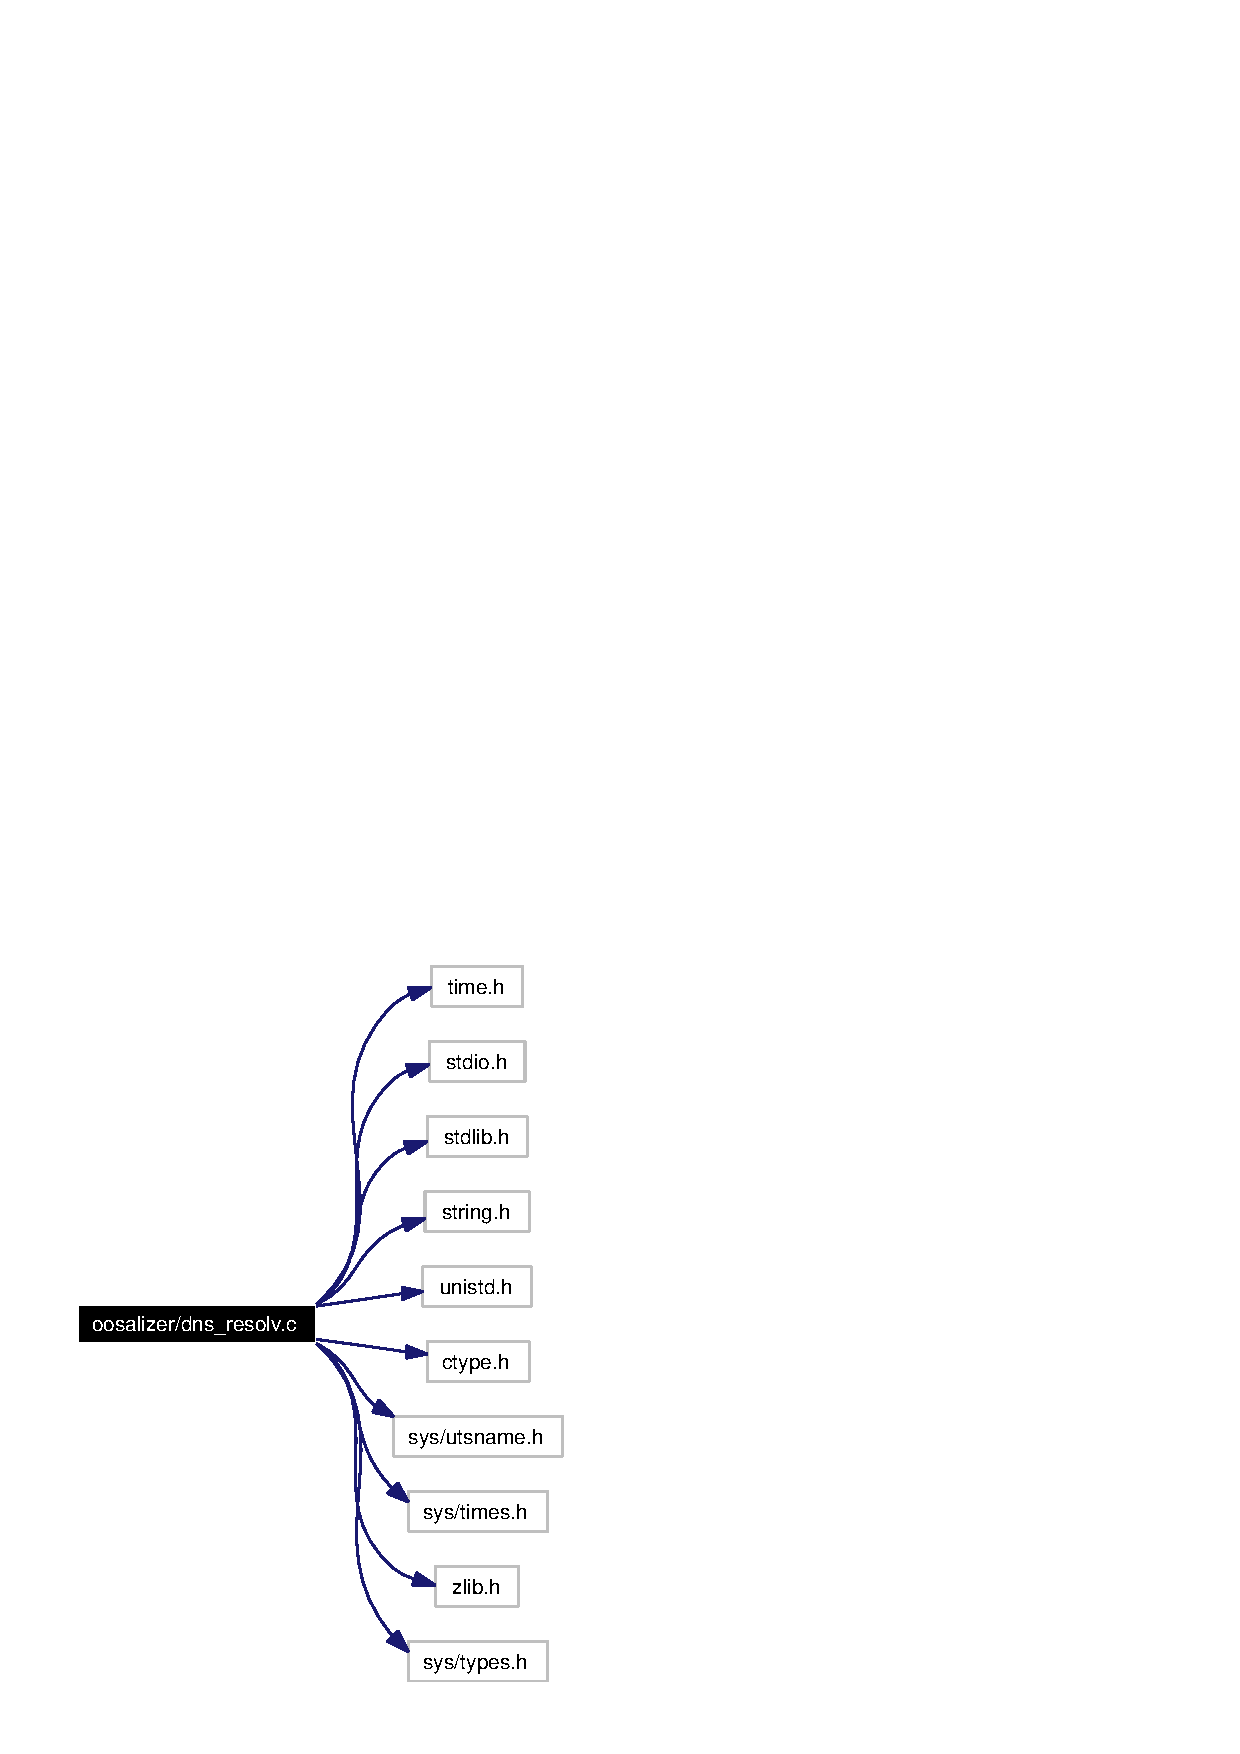
\includegraphics[width=135pt]{dns__resolv_8c__incl}
\end{center}
\end{figure}
\subsection*{Makrodefinitionen}
\begin{CompactItemize}
\item 
\#define {\bf CLK\_\-TCK}~\_\-SC\_\-CLK\_\-TCK
\end{CompactItemize}


\subsection{Makro-Dokumentation}
\index{dns_resolv.c@{dns\_\-resolv.c}!CLK_TCK@{CLK\_\-TCK}}
\index{CLK_TCK@{CLK\_\-TCK}!dns_resolv.c@{dns\_\-resolv.c}}
\subsubsection{\setlength{\rightskip}{0pt plus 5cm}\#define CLK\_\-TCK~\_\-SC\_\-CLK\_\-TCK}\label{dns__resolv_8c_03df76d1f70664d745ca8de2864e39b3}




Definiert in Zeile 71 der Datei dns\_\-resolv.c.
\section{oosalizer/dns\_\-resolv.h-Dateireferenz}
\label{dns__resolv_8h}\index{oosalizer/dns_resolv.h@{oosalizer/dns\_\-resolv.h}}

\section{oosalizer/graphs.c-Dateireferenz}
\label{graphs_8c}\index{oosalizer/graphs.c@{oosalizer/graphs.c}}
{\tt \#include $<$math.h$>$}\par
{\tt \#include $<$stdio.h$>$}\par
{\tt \#include $<$string.h$>$}\par
{\tt \#include $<$sys/types.h$>$}\par
{\tt \#include $<$gd.h$>$}\par
{\tt \#include $<$gdfontt.h$>$}\par
{\tt \#include $<$gdfonts.h$>$}\par
{\tt \#include $<$gdfontmb.h$>$}\par
{\tt \#include \char`\"{}webalizer.h\char`\"{}}\par
{\tt \#include \char`\"{}lang.h\char`\"{}}\par
{\tt \#include \char`\"{}graphs.h\char`\"{}}\par


Include-Abh\"{a}ngigkeitsdiagramm f\"{u}r graphs.c:\begin{figure}[H]
\begin{center}
\leavevmode
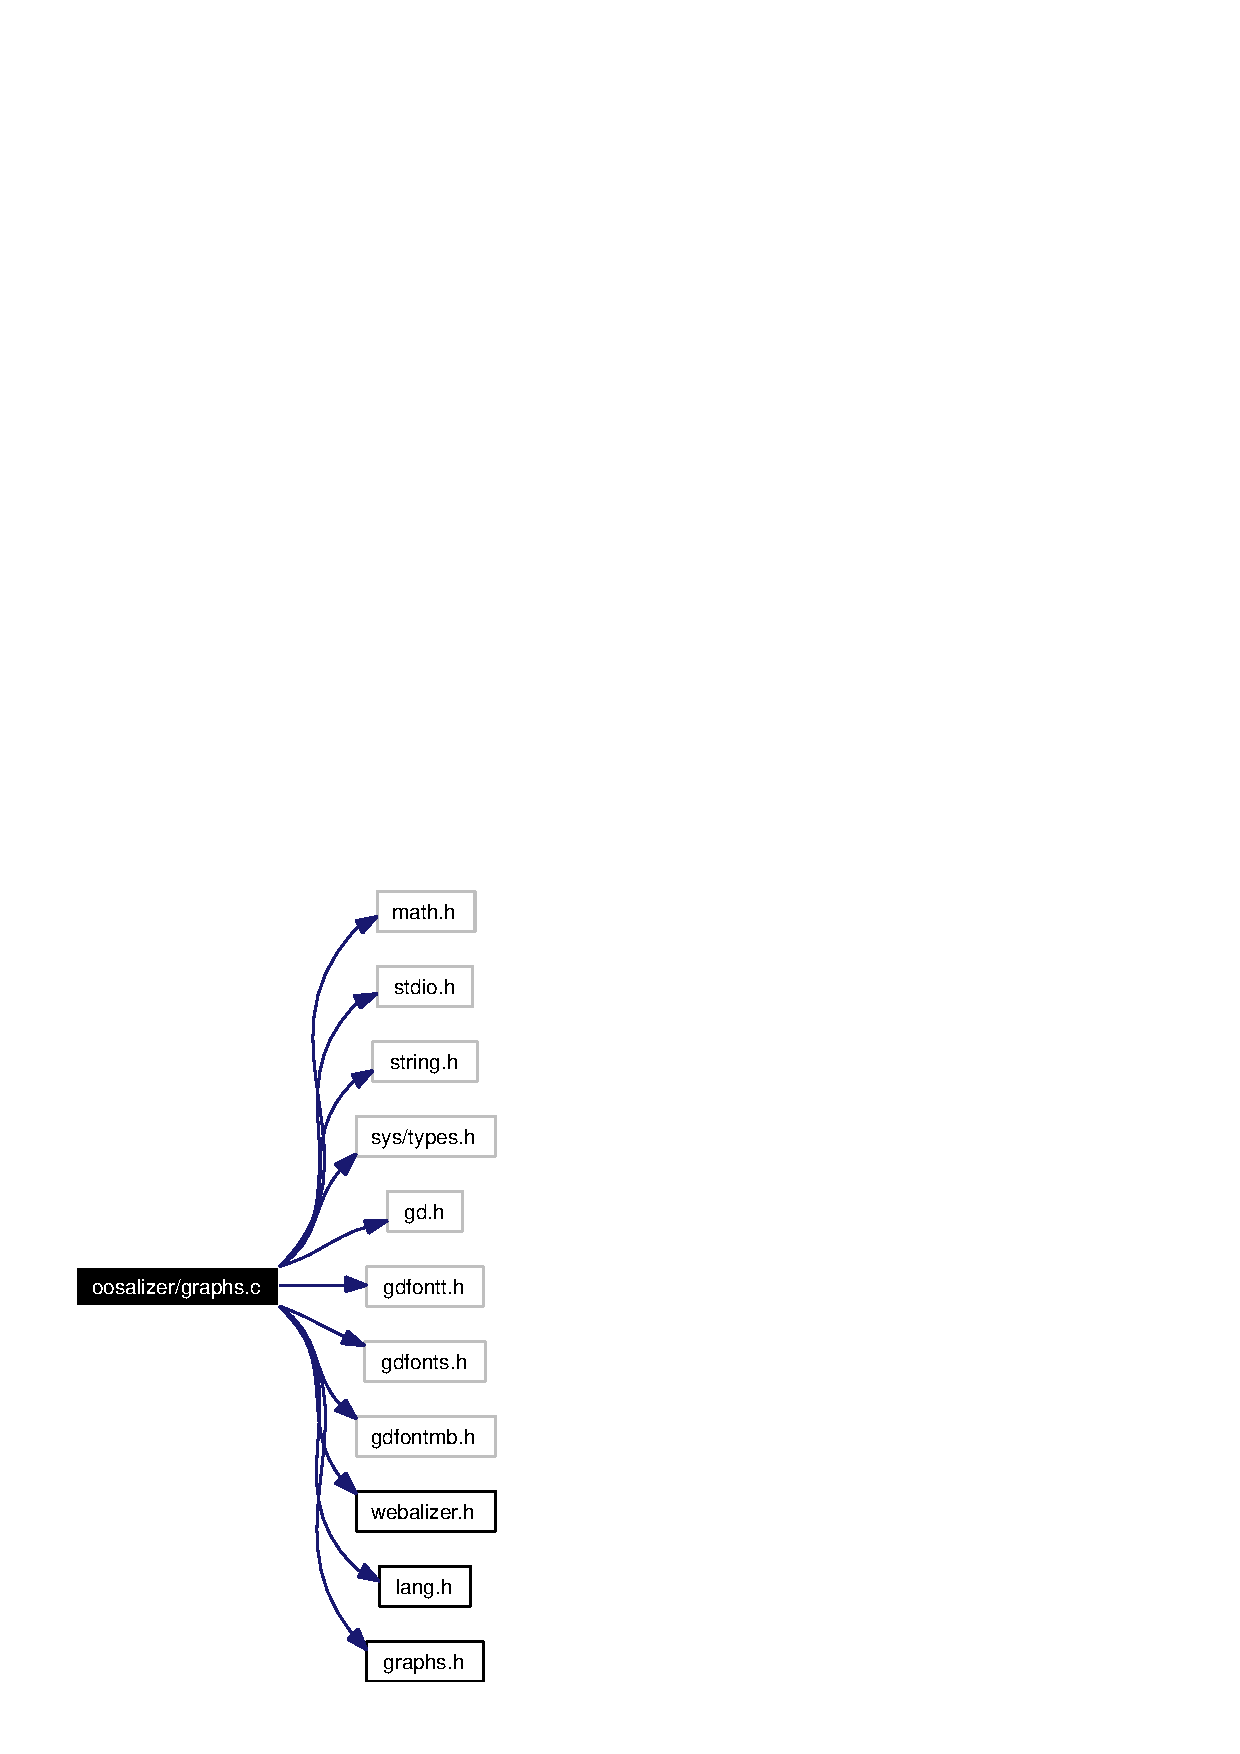
\includegraphics[width=119pt]{graphs_8c__incl}
\end{center}
\end{figure}
\subsection*{Datenstrukturen}
\begin{CompactItemize}
\item 
struct {\bf pie\_\-data}
\end{CompactItemize}
\subsection*{Makrodefinitionen}
\begin{CompactItemize}
\item 
\#define {\bf PI}~3.14159265358979323846
\item 
\#define {\bf COLOR1}~{\bf green}
\item 
\#define {\bf COLOR2}~{\bf blue}
\item 
\#define {\bf COLOR3}~{\bf orange}
\item 
\#define {\bf COLOR4}~{\bf red}
\item 
\#define {\bf COLOR5}~{\bf cyan}
\item 
\#define {\bf COLOR6}~{\bf yellow}
\item 
\#define {\bf CX}~156
\item 
\#define {\bf CY}~150
\item 
\#define {\bf XRAD}~240
\item 
\#define {\bf YRAD}~200
\item 
\#define {\bf YSIZE}~400
\end{CompactItemize}
\subsection*{Funktionen}
\begin{CompactItemize}
\item 
void {\bf init\_\-graph} (char $\ast$, int, int)
\item 
{\bf pie\_\-data} $\ast$ {\bf calc\_\-arc} (float, float)
\item 
int {\bf year\_\-graph6x} (char $\ast$fname, char $\ast$title, int fmonth, u\_\-long data1[12], u\_\-long data2[12], u\_\-long data3[12], double data4[12], u\_\-long data5[12], u\_\-long data6[12])
\item 
int {\bf month\_\-graph6} (char $\ast$fname, char $\ast$title, int month, int year, u\_\-long data1[31], u\_\-long data2[31], u\_\-long data3[31], double data4[31], u\_\-long data5[31], u\_\-long data6[31])
\item 
int {\bf day\_\-graph3} (char $\ast$fname, char $\ast$title, u\_\-long data1[24], u\_\-long data2[24], u\_\-long data3[24])
\item 
int {\bf pie\_\-chart} (char $\ast$fname, char $\ast$title, u\_\-long t\_\-val, u\_\-long data1[$\,$], char $\ast$legend[$\,$])
\end{CompactItemize}
\subsection*{Variablen}
\begin{CompactItemize}
\item 
char $\ast$ {\bf numchar} [$\,$]
\item 
gd\-Image\-Ptr {\bf im}
\item 
FILE $\ast$ {\bf out}
\item 
char {\bf maxvaltxt} [32]
\item 
float {\bf percent}
\item 
u\_\-long {\bf julday}
\item 
int {\bf black}
\item 
int {\bf white}
\item 
int {\bf grey}
\item 
int {\bf dkgrey}
\item 
int {\bf red}
\item 
int {\bf blue}
\item 
int {\bf orange}
\item 
int {\bf green}
\item 
int {\bf cyan}
\item 
int {\bf yellow}
\end{CompactItemize}


\subsection{Makro-Dokumentation}
\index{graphs.c@{graphs.c}!COLOR1@{COLOR1}}
\index{COLOR1@{COLOR1}!graphs.c@{graphs.c}}
\subsubsection{\setlength{\rightskip}{0pt plus 5cm}\#define COLOR1~{\bf green}}\label{graphs_8c_1169cd1b397420b29bd3b0153f047818}




Definiert in Zeile 47 der Datei graphs.c.

Wird benutzt von month\_\-graph6().\index{graphs.c@{graphs.c}!COLOR2@{COLOR2}}
\index{COLOR2@{COLOR2}!graphs.c@{graphs.c}}
\subsubsection{\setlength{\rightskip}{0pt plus 5cm}\#define COLOR2~{\bf blue}}\label{graphs_8c_609e0791889f4cde446ee0eb6efd369a}




Definiert in Zeile 48 der Datei graphs.c.\index{graphs.c@{graphs.c}!COLOR3@{COLOR3}}
\index{COLOR3@{COLOR3}!graphs.c@{graphs.c}}
\subsubsection{\setlength{\rightskip}{0pt plus 5cm}\#define COLOR3~{\bf orange}}\label{graphs_8c_299edc84540341c664cd7a183e8fc9bd}




Definiert in Zeile 49 der Datei graphs.c.\index{graphs.c@{graphs.c}!COLOR4@{COLOR4}}
\index{COLOR4@{COLOR4}!graphs.c@{graphs.c}}
\subsubsection{\setlength{\rightskip}{0pt plus 5cm}\#define COLOR4~{\bf red}}\label{graphs_8c_5b1074ec004e850c360022e0d433e475}




Definiert in Zeile 50 der Datei graphs.c.\index{graphs.c@{graphs.c}!COLOR5@{COLOR5}}
\index{COLOR5@{COLOR5}!graphs.c@{graphs.c}}
\subsubsection{\setlength{\rightskip}{0pt plus 5cm}\#define COLOR5~{\bf cyan}}\label{graphs_8c_b1b154af4927f41dc0ac230992bf1a15}




Definiert in Zeile 51 der Datei graphs.c.\index{graphs.c@{graphs.c}!COLOR6@{COLOR6}}
\index{COLOR6@{COLOR6}!graphs.c@{graphs.c}}
\subsubsection{\setlength{\rightskip}{0pt plus 5cm}\#define COLOR6~{\bf yellow}}\label{graphs_8c_8fd4fb399b4659d7aed1fcb5cc182ebb}




Definiert in Zeile 52 der Datei graphs.c.\index{graphs.c@{graphs.c}!CX@{CX}}
\index{CX@{CX}!graphs.c@{graphs.c}}
\subsubsection{\setlength{\rightskip}{0pt plus 5cm}\#define CX~156}\label{graphs_8c_0b4c12a5dc8490a3cff8385334db2d13}




Definiert in Zeile 54 der Datei graphs.c.

Wird benutzt von calc\_\-arc() und pie\_\-chart().\index{graphs.c@{graphs.c}!CY@{CY}}
\index{CY@{CY}!graphs.c@{graphs.c}}
\subsubsection{\setlength{\rightskip}{0pt plus 5cm}\#define CY~150}\label{graphs_8c_c5bc792e372b15e7a1d3efe6daac9aec}




Definiert in Zeile 55 der Datei graphs.c.

Wird benutzt von calc\_\-arc() und pie\_\-chart().\index{graphs.c@{graphs.c}!PI@{PI}}
\index{PI@{PI}!graphs.c@{graphs.c}}
\subsubsection{\setlength{\rightskip}{0pt plus 5cm}\#define PI~3.14159265358979323846}\label{graphs_8c_598a3330b3c21701223ee0ca14316eca}




Definiert in Zeile 44 der Datei graphs.c.

Wird benutzt von calc\_\-arc().\index{graphs.c@{graphs.c}!XRAD@{XRAD}}
\index{XRAD@{XRAD}!graphs.c@{graphs.c}}
\subsubsection{\setlength{\rightskip}{0pt plus 5cm}\#define XRAD~240}\label{graphs_8c_e1eec295ea8cd8f04c1f24b59110fcae}




Definiert in Zeile 56 der Datei graphs.c.

Wird benutzt von calc\_\-arc() und pie\_\-chart().\index{graphs.c@{graphs.c}!YRAD@{YRAD}}
\index{YRAD@{YRAD}!graphs.c@{graphs.c}}
\subsubsection{\setlength{\rightskip}{0pt plus 5cm}\#define YRAD~200}\label{graphs_8c_3eeb4d5b339574d992e5ac5b2c5cd8ff}




Definiert in Zeile 57 der Datei graphs.c.

Wird benutzt von calc\_\-arc() und pie\_\-chart().\index{graphs.c@{graphs.c}!YSIZE@{YSIZE}}
\index{YSIZE@{YSIZE}!graphs.c@{graphs.c}}
\subsubsection{\setlength{\rightskip}{0pt plus 5cm}\#define YSIZE~400}\label{graphs_8c_faefa0d521156ca605f526c14d05e272}




Definiert in Zeile 296 der Datei graphs.c.

\subsection{Dokumentation der Funktionen}
\index{graphs.c@{graphs.c}!calc_arc@{calc\_\-arc}}
\index{calc_arc@{calc\_\-arc}!graphs.c@{graphs.c}}
\subsubsection{\setlength{\rightskip}{0pt plus 5cm}struct {\bf pie\_\-data} $\ast$ calc\_\-arc (float, float)}\label{graphs_8c_b831d5a0b0198ea523e0b116aaa20488}




Definiert in Zeile 694 der Datei graphs.c.

Benutzt CX, CY, pie\_\-data::mx, pie\_\-data::my, PI, pie\_\-data::x, XRAD, pie\_\-data::y und YRAD.

Wird benutzt von pie\_\-chart().\index{graphs.c@{graphs.c}!day_graph3@{day\_\-graph3}}
\index{day_graph3@{day\_\-graph3}!graphs.c@{graphs.c}}
\subsubsection{\setlength{\rightskip}{0pt plus 5cm}int day\_\-graph3 (char $\ast$ {\em fname}, char $\ast$ {\em title}, u\_\-long {\em data1}[24], u\_\-long {\em data2}[24], u\_\-long {\em data3}[24])}\label{graphs_8c_98296b41d7e2982e4b341e6ed18255ac}




Definiert in Zeile 503 der Datei graphs.c.

Benutzt black, dkgrey, graph\_\-lines, im, init\_\-graph() und numchar.

Wird benutzt von write\_\-month\_\-html().\index{graphs.c@{graphs.c}!init_graph@{init\_\-graph}}
\index{init_graph@{init\_\-graph}!graphs.c@{graphs.c}}
\subsubsection{\setlength{\rightskip}{0pt plus 5cm}void init\_\-graph (char $\ast$, int, int)}\label{graphs_8c_2040d817b934e470b4a2cdeb9811c097}




Definiert in Zeile 716 der Datei graphs.c.

Benutzt black, blue, cyan, dkgrey, green, grey, im, orange, red, white und yellow.

Wird benutzt von day\_\-graph3(), month\_\-graph6(), pie\_\-chart() und year\_\-graph6x().\index{graphs.c@{graphs.c}!month_graph6@{month\_\-graph6}}
\index{month_graph6@{month\_\-graph6}!graphs.c@{graphs.c}}
\subsubsection{\setlength{\rightskip}{0pt plus 5cm}int month\_\-graph6 (char $\ast$ {\em fname}, char $\ast$ {\em title}, int {\em month}, int {\em year}, u\_\-long {\em data1}[31], u\_\-long {\em data2}[31], u\_\-long {\em data3}[31], double {\em data4}[31], u\_\-long {\em data5}[31], u\_\-long {\em data6}[31])}\label{graphs_8c_7d33e4e14ae660bf05b5793f8e18d091}




Definiert in Zeile 298 der Datei graphs.c.

Benutzt black, COLOR1, dkgrey, graph\_\-lines, im, init\_\-graph(), jdate(), julday, numchar und white.

Wird benutzt von write\_\-month\_\-html().\index{graphs.c@{graphs.c}!pie_chart@{pie\_\-chart}}
\index{pie_chart@{pie\_\-chart}!graphs.c@{graphs.c}}
\subsubsection{\setlength{\rightskip}{0pt plus 5cm}int pie\_\-chart (char $\ast$ {\em fname}, char $\ast$ {\em title}, u\_\-long {\em t\_\-val}, u\_\-long {\em data1}[$\,$], char $\ast$ {\em legend}[$\,$])}\label{graphs_8c_49e615d9104950eeb7a886df4301f7da}




Definiert in Zeile 610 der Datei graphs.c.

Benutzt black, buffer, calc\_\-arc(), CX, CY, im, init\_\-graph(), percent, pie\_\-data::x, XRAD, pie\_\-data::y und YRAD.\index{graphs.c@{graphs.c}!year_graph6x@{year\_\-graph6x}}
\index{year_graph6x@{year\_\-graph6x}!graphs.c@{graphs.c}}
\subsubsection{\setlength{\rightskip}{0pt plus 5cm}int year\_\-graph6x (char $\ast$ {\em fname}, char $\ast$ {\em title}, int {\em fmonth}, u\_\-long {\em data1}[12], u\_\-long {\em data2}[12], u\_\-long {\em data3}[12], double {\em data4}[12], u\_\-long {\em data5}[12], u\_\-long {\em data6}[12])}\label{graphs_8c_58eec29feb4d1c90de8813c8c59d4fcd}




Definiert in Zeile 88 der Datei graphs.c.

Benutzt black, dkgrey, graph\_\-lines, im, init\_\-graph(), s\_\-month und white.

\subsection{Variablen-Dokumentation}
\index{graphs.c@{graphs.c}!black@{black}}
\index{black@{black}!graphs.c@{graphs.c}}
\subsubsection{\setlength{\rightskip}{0pt plus 5cm}int {\bf black}}\label{graphs_8c_8784d4f8ed73cff78355d2ed8e0c3a3b}




Definiert in Zeile 79 der Datei graphs.c.

Wird benutzt von day\_\-graph3(), init\_\-graph(), month\_\-graph6(), pie\_\-chart() und year\_\-graph6x().\index{graphs.c@{graphs.c}!blue@{blue}}
\index{blue@{blue}!graphs.c@{graphs.c}}
\subsubsection{\setlength{\rightskip}{0pt plus 5cm}int {\bf blue}}\label{graphs_8c_16043f28bf0a6b55db852853f0683fc2}




Definiert in Zeile 79 der Datei graphs.c.

Wird benutzt von init\_\-graph().\index{graphs.c@{graphs.c}!cyan@{cyan}}
\index{cyan@{cyan}!graphs.c@{graphs.c}}
\subsubsection{\setlength{\rightskip}{0pt plus 5cm}int {\bf cyan}}\label{graphs_8c_f6bc84de5c6f5361f222772133cf1ab8}




Definiert in Zeile 79 der Datei graphs.c.

Wird benutzt von init\_\-graph().\index{graphs.c@{graphs.c}!dkgrey@{dkgrey}}
\index{dkgrey@{dkgrey}!graphs.c@{graphs.c}}
\subsubsection{\setlength{\rightskip}{0pt plus 5cm}int {\bf dkgrey}}\label{graphs_8c_ee1005868568d9750214235693ba63e1}




Definiert in Zeile 79 der Datei graphs.c.

Wird benutzt von day\_\-graph3(), init\_\-graph(), month\_\-graph6() und year\_\-graph6x().\index{graphs.c@{graphs.c}!green@{green}}
\index{green@{green}!graphs.c@{graphs.c}}
\subsubsection{\setlength{\rightskip}{0pt plus 5cm}int {\bf green}}\label{graphs_8c_6e208843f894f38fa7644608917a2a41}




Definiert in Zeile 79 der Datei graphs.c.

Wird benutzt von init\_\-graph().\index{graphs.c@{graphs.c}!grey@{grey}}
\index{grey@{grey}!graphs.c@{graphs.c}}
\subsubsection{\setlength{\rightskip}{0pt plus 5cm}int {\bf grey}}\label{graphs_8c_852d2c8c77477e510b44d799fdaaf1f9}




Definiert in Zeile 79 der Datei graphs.c.

Wird benutzt von init\_\-graph().\index{graphs.c@{graphs.c}!im@{im}}
\index{im@{im}!graphs.c@{graphs.c}}
\subsubsection{\setlength{\rightskip}{0pt plus 5cm}gd\-Image\-Ptr {\bf im}}\label{graphs_8c_0e84b6d886b70b0cf21c56e5e26f0ed9}




Definiert in Zeile 70 der Datei graphs.c.

Wird benutzt von day\_\-graph3(), init\_\-graph(), month\_\-graph6(), pie\_\-chart() und year\_\-graph6x().\index{graphs.c@{graphs.c}!julday@{julday}}
\index{julday@{julday}!graphs.c@{graphs.c}}
\subsubsection{\setlength{\rightskip}{0pt plus 5cm}u\_\-long {\bf julday}}\label{graphs_8c_488cb40243821792a9a226ca1042b3e1}




Definiert in Zeile 74 der Datei graphs.c.

Wird benutzt von month\_\-graph6().\index{graphs.c@{graphs.c}!maxvaltxt@{maxvaltxt}}
\index{maxvaltxt@{maxvaltxt}!graphs.c@{graphs.c}}
\subsubsection{\setlength{\rightskip}{0pt plus 5cm}char {\bf maxvaltxt}[32]}\label{graphs_8c_3933b61d12d9878aa33d711259d94c5f}




Definiert in Zeile 72 der Datei graphs.c.\index{graphs.c@{graphs.c}!numchar@{numchar}}
\index{numchar@{numchar}!graphs.c@{graphs.c}}
\subsubsection{\setlength{\rightskip}{0pt plus 5cm}char$\ast$ {\bf numchar}[$\,$]}\label{graphs_8c_d8920ceda92347671d37ba01be631d65}


{\bf Initialisierung:}

\footnotesize\begin{verbatim} { " 0"," 1"," 2"," 3"," 4"," 5"," 6"," 7"," 8"," 9","10",
                    "11","12","13","14","15","16","17","18","19","20",
                    "21","22","23","24","25","26","27","28","29","30","31"}
\end{verbatim}\normalsize 


Definiert in Zeile 66 der Datei graphs.c.

Wird benutzt von day\_\-graph3() und month\_\-graph6().\index{graphs.c@{graphs.c}!orange@{orange}}
\index{orange@{orange}!graphs.c@{graphs.c}}
\subsubsection{\setlength{\rightskip}{0pt plus 5cm}int {\bf orange}}\label{graphs_8c_d316f80317cb97c5ada72ac0e05bbf92}




Definiert in Zeile 79 der Datei graphs.c.

Wird benutzt von init\_\-graph().\index{graphs.c@{graphs.c}!out@{out}}
\index{out@{out}!graphs.c@{graphs.c}}
\subsubsection{\setlength{\rightskip}{0pt plus 5cm}FILE$\ast$ {\bf out}}\label{graphs_8c_1277960b5f2b37137fe9b0b5a1ea0beb}




Definiert in Zeile 71 der Datei graphs.c.\index{graphs.c@{graphs.c}!percent@{percent}}
\index{percent@{percent}!graphs.c@{graphs.c}}
\subsubsection{\setlength{\rightskip}{0pt plus 5cm}float {\bf percent}}\label{graphs_8c_ac167f3972a2f244f4b32c8ee5b89364}




Definiert in Zeile 73 der Datei graphs.c.

Wird benutzt von pie\_\-chart().\index{graphs.c@{graphs.c}!red@{red}}
\index{red@{red}!graphs.c@{graphs.c}}
\subsubsection{\setlength{\rightskip}{0pt plus 5cm}int {\bf red}}\label{graphs_8c_6761340706096510fd89edca40a63b9b}




Definiert in Zeile 79 der Datei graphs.c.

Wird benutzt von init\_\-graph().\index{graphs.c@{graphs.c}!white@{white}}
\index{white@{white}!graphs.c@{graphs.c}}
\subsubsection{\setlength{\rightskip}{0pt plus 5cm}int {\bf white}}\label{graphs_8c_52b8a1dc217164197e6e5ba60ec911bf}




Definiert in Zeile 79 der Datei graphs.c.

Wird benutzt von init\_\-graph(), month\_\-graph6() und year\_\-graph6x().\index{graphs.c@{graphs.c}!yellow@{yellow}}
\index{yellow@{yellow}!graphs.c@{graphs.c}}
\subsubsection{\setlength{\rightskip}{0pt plus 5cm}int {\bf yellow}}\label{graphs_8c_34167711871149458e41ef5d3e3541fe}




Definiert in Zeile 79 der Datei graphs.c.

Wird benutzt von init\_\-graph().
\section{oosalizer/graphs.h-Dateireferenz}
\label{graphs_8h}\index{oosalizer/graphs.h@{oosalizer/graphs.h}}


Dieser Graph zeigt, welche Datei direkt oder indirekt diese Datei enth\"{a}lt:\begin{figure}[H]
\begin{center}
\leavevmode
\includegraphics[width=134pt]{graphs_8h__dep__incl}
\end{center}
\end{figure}
\subsection*{Funktionen}
\begin{CompactItemize}
\item 
int {\bf month\_\-graph6} (char $\ast$, char $\ast$, int, int, u\_\-long $\ast$, u\_\-long $\ast$, u\_\-long $\ast$, double $\ast$, u\_\-long $\ast$, u\_\-long $\ast$)
\item 
int {\bf year\_\-graph6x} (char $\ast$, char $\ast$, int, u\_\-long $\ast$, u\_\-long $\ast$, u\_\-long $\ast$, double $\ast$, u\_\-long $\ast$, u\_\-long $\ast$)
\item 
int {\bf day\_\-graph3} (char $\ast$, char $\ast$, u\_\-long $\ast$, u\_\-long $\ast$, u\_\-long $\ast$)
\item 
int {\bf pie\_\-chart} (char $\ast$, char $\ast$, u\_\-long, u\_\-long $\ast$, char $\ast$$\ast$)
\end{CompactItemize}


\subsection{Dokumentation der Funktionen}
\index{graphs.h@{graphs.h}!day_graph3@{day\_\-graph3}}
\index{day_graph3@{day\_\-graph3}!graphs.h@{graphs.h}}
\subsubsection{\setlength{\rightskip}{0pt plus 5cm}int day\_\-graph3 (char $\ast$, char $\ast$, u\_\-long $\ast$, u\_\-long $\ast$, u\_\-long $\ast$)}\label{graphs_8h_0aac6a5e38fa2280a1fc65b1387f3bbf}


\index{graphs.h@{graphs.h}!month_graph6@{month\_\-graph6}}
\index{month_graph6@{month\_\-graph6}!graphs.h@{graphs.h}}
\subsubsection{\setlength{\rightskip}{0pt plus 5cm}int month\_\-graph6 (char $\ast$, char $\ast$, int, int, u\_\-long $\ast$, u\_\-long $\ast$, u\_\-long $\ast$, double $\ast$, u\_\-long $\ast$, u\_\-long $\ast$)}\label{graphs_8h_5162657b4dcc3453169c3275c52932ea}


\index{graphs.h@{graphs.h}!pie_chart@{pie\_\-chart}}
\index{pie_chart@{pie\_\-chart}!graphs.h@{graphs.h}}
\subsubsection{\setlength{\rightskip}{0pt plus 5cm}int pie\_\-chart (char $\ast$, char $\ast$, u\_\-long, u\_\-long $\ast$, char $\ast$$\ast$)}\label{graphs_8h_59a8251be3cd0f8b093804b60c08111e}


\index{graphs.h@{graphs.h}!year_graph6x@{year\_\-graph6x}}
\index{year_graph6x@{year\_\-graph6x}!graphs.h@{graphs.h}}
\subsubsection{\setlength{\rightskip}{0pt plus 5cm}int year\_\-graph6x (char $\ast$, char $\ast$, int, u\_\-long $\ast$, u\_\-long $\ast$, u\_\-long $\ast$, double $\ast$, u\_\-long $\ast$, u\_\-long $\ast$)}\label{graphs_8h_535fbbd777a3b3e4b015be7fe923c83a}



\section{oosalizer/hashtab.c-Dateireferenz}
\label{hashtab_8c}\index{oosalizer/hashtab.c@{oosalizer/hashtab.c}}
{\tt \#include $<$time.h$>$}\par
{\tt \#include $<$stdio.h$>$}\par
{\tt \#include $<$stdlib.h$>$}\par
{\tt \#include $<$string.h$>$}\par
{\tt \#include $<$unistd.h$>$}\par
{\tt \#include $<$ctype.h$>$}\par
{\tt \#include $<$sys/utsname.h$>$}\par
{\tt \#include $<$sys/times.h$>$}\par
{\tt \#include $<$sys/types.h$>$}\par
{\tt \#include \char`\"{}webalizer.h\char`\"{}}\par
{\tt \#include \char`\"{}lang.h\char`\"{}}\par
{\tt \#include \char`\"{}linklist.h\char`\"{}}\par
{\tt \#include \char`\"{}hashtab.h\char`\"{}}\par


Include-Abh\"{a}ngigkeitsdiagramm f\"{u}r hashtab.c:\begin{figure}[H]
\begin{center}
\leavevmode
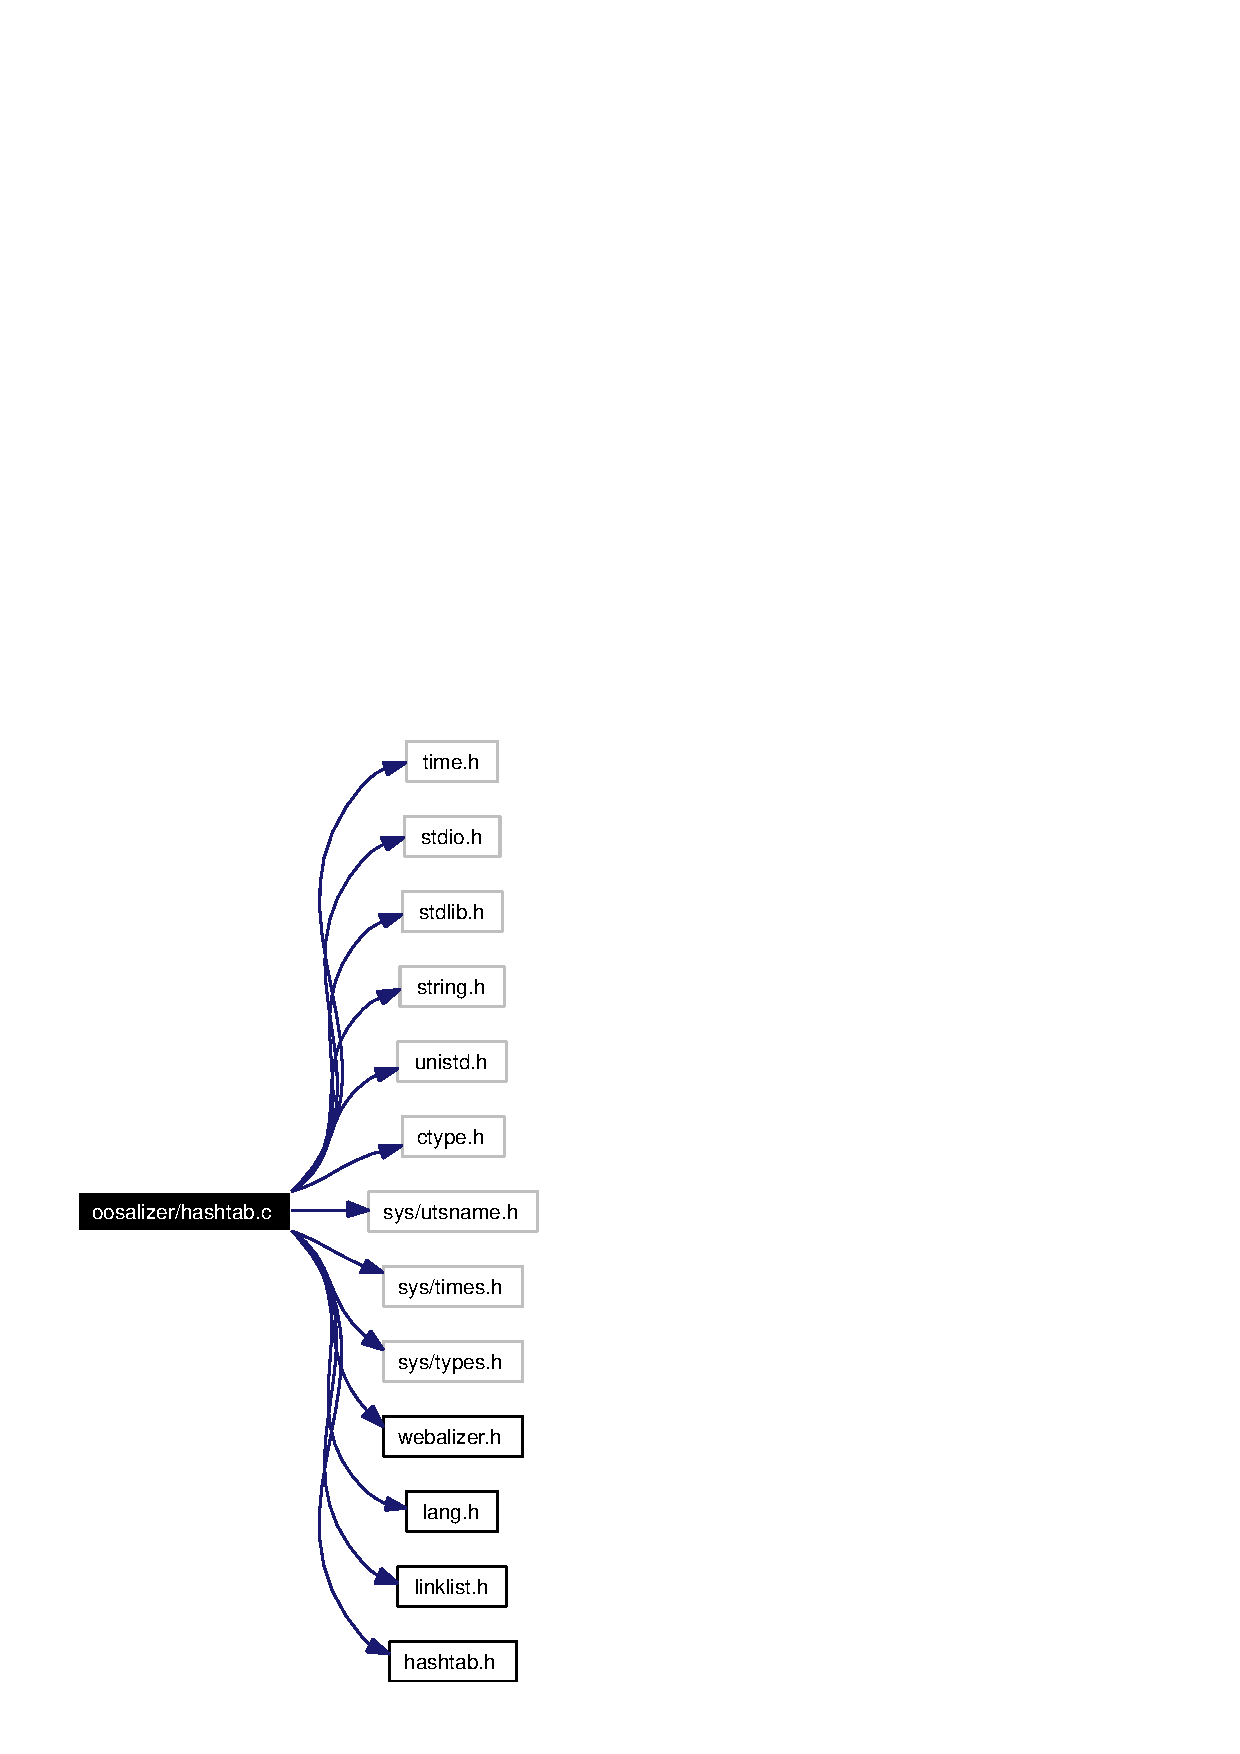
\includegraphics[width=129pt]{hashtab_8c__incl}
\end{center}
\end{figure}
\subsection*{Makrodefinitionen}
\begin{CompactItemize}
\item 
\#define {\bf CLK\_\-TCK}~\_\-SC\_\-CLK\_\-TCK
\end{CompactItemize}
\subsection*{Funktionen}
\begin{CompactItemize}
\item 
{\bf HNODEPTR} {\bf new\_\-hnode} (char $\ast$)
\item 
{\bf UNODEPTR} {\bf new\_\-unode} (char $\ast$)
\item 
{\bf RNODEPTR} {\bf new\_\-rnode} (char $\ast$)
\item 
{\bf ANODEPTR} {\bf new\_\-anode} (char $\ast$)
\item 
{\bf SNODEPTR} {\bf new\_\-snode} (char $\ast$)
\item 
{\bf INODEPTR} {\bf new\_\-inode} (char $\ast$)
\item 
void {\bf update\_\-entry} (char $\ast$)
\item 
void {\bf update\_\-exit} (char $\ast$)
\item 
u\_\-long {\bf hash} (char $\ast$)
\item 
void {\bf del\_\-htabs} ()
\item 
int {\bf put\_\-hnode} (char $\ast$str, int type, u\_\-long count, u\_\-long file, double xfer, u\_\-long $\ast$ctr, u\_\-long visit, u\_\-long tstamp, char $\ast$lasturl, {\bf HNODEPTR} $\ast$htab)
\item 
void {\bf del\_\-hlist} ({\bf HNODEPTR} $\ast$htab)
\item 
int {\bf put\_\-unode} (char $\ast$str, int type, u\_\-long count, double xfer, u\_\-long $\ast$ctr, u\_\-long entry, u\_\-long exit, {\bf UNODEPTR} $\ast$htab)
\item 
void {\bf del\_\-ulist} ({\bf UNODEPTR} $\ast$htab)
\item 
int {\bf put\_\-rnode} (char $\ast$str, int type, u\_\-long count, u\_\-long $\ast$ctr, {\bf RNODEPTR} $\ast$htab)
\item 
void {\bf del\_\-rlist} ({\bf RNODEPTR} $\ast$htab)
\item 
int {\bf put\_\-anode} (char $\ast$str, int type, u\_\-long count, u\_\-long $\ast$ctr, {\bf ANODEPTR} $\ast$htab)
\item 
void {\bf del\_\-alist} ({\bf ANODEPTR} $\ast$htab)
\item 
int {\bf put\_\-snode} (char $\ast$str, u\_\-long count, {\bf SNODEPTR} $\ast$htab)
\item 
void {\bf del\_\-slist} ({\bf SNODEPTR} $\ast$htab)
\item 
int {\bf put\_\-inode} (char $\ast$str, int type, u\_\-long count, u\_\-long file, double xfer, u\_\-long $\ast$ctr, u\_\-long visit, u\_\-long tstamp, {\bf INODEPTR} $\ast$htab)
\item 
void {\bf del\_\-ilist} ({\bf INODEPTR} $\ast$htab)
\item 
char $\ast$ {\bf find\_\-url} (char $\ast$str)
\item 
void {\bf month\_\-update\_\-exit} (u\_\-long tstamp)
\item 
u\_\-long {\bf tot\_\-visit} ({\bf HNODEPTR} $\ast$list)
\end{CompactItemize}
\subsection*{Variablen}
\begin{CompactItemize}
\item 
{\bf HNODEPTR} {\bf sm\_\-htab} [MAXHASH]
\item 
{\bf HNODEPTR} {\bf sd\_\-htab} [MAXHASH]
\item 
{\bf UNODEPTR} {\bf um\_\-htab} [MAXHASH]
\item 
{\bf RNODEPTR} {\bf rm\_\-htab} [MAXHASH]
\item 
{\bf ANODEPTR} {\bf am\_\-htab} [MAXHASH]
\item 
{\bf SNODEPTR} {\bf sr\_\-htab} [MAXHASH]
\item 
{\bf INODEPTR} {\bf im\_\-htab} [MAXHASH]
\end{CompactItemize}


\subsection{Makro-Dokumentation}
\index{hashtab.c@{hashtab.c}!CLK_TCK@{CLK\_\-TCK}}
\index{CLK_TCK@{CLK\_\-TCK}!hashtab.c@{hashtab.c}}
\subsubsection{\setlength{\rightskip}{0pt plus 5cm}\#define CLK\_\-TCK~\_\-SC\_\-CLK\_\-TCK}\label{hashtab_8c_03df76d1f70664d745ca8de2864e39b3}




Definiert in Zeile 59 der Datei hashtab.c.

\subsection{Dokumentation der Funktionen}
\index{hashtab.c@{hashtab.c}!del_alist@{del\_\-alist}}
\index{del_alist@{del\_\-alist}!hashtab.c@{hashtab.c}}
\subsubsection{\setlength{\rightskip}{0pt plus 5cm}void del\_\-alist ({\bf ANODEPTR} $\ast$ {\em htab})}\label{hashtab_8c_ebb84eee637f50db17ab93d1050e8bd1}




Definiert in Zeile 645 der Datei hashtab.c.

Benutzt MAXHASH, anode::next und anode::string.

Wird benutzt von del\_\-htabs().\index{hashtab.c@{hashtab.c}!del_hlist@{del\_\-hlist}}
\index{del_hlist@{del\_\-hlist}!hashtab.c@{hashtab.c}}
\subsubsection{\setlength{\rightskip}{0pt plus 5cm}void del\_\-hlist ({\bf HNODEPTR} $\ast$ {\em htab})}\label{hashtab_8c_306d5a1540d43fa136c10272cb2f0a4a}




Definiert in Zeile 283 der Datei hashtab.c.

Benutzt MAXHASH, hnode::next und hnode::string.

Wird benutzt von del\_\-htabs().\index{hashtab.c@{hashtab.c}!del_htabs@{del\_\-htabs}}
\index{del_htabs@{del\_\-htabs}!hashtab.c@{hashtab.c}}
\subsubsection{\setlength{\rightskip}{0pt plus 5cm}void del\_\-htabs ()}\label{hashtab_8c_f9fcdad76e91434fe5f0728f3a79ae74}




Definiert in Zeile 102 der Datei hashtab.c.

Benutzt am\_\-htab, del\_\-alist(), del\_\-hlist(), del\_\-ilist(), del\_\-rlist(), del\_\-slist(), del\_\-ulist(), im\_\-htab, rm\_\-htab, sd\_\-htab, sm\_\-htab, sr\_\-htab und um\_\-htab.

Wird benutzt von clear\_\-month().\index{hashtab.c@{hashtab.c}!del_ilist@{del\_\-ilist}}
\index{del_ilist@{del\_\-ilist}!hashtab.c@{hashtab.c}}
\subsubsection{\setlength{\rightskip}{0pt plus 5cm}void del\_\-ilist ({\bf INODEPTR} $\ast$ {\em htab})}\label{hashtab_8c_d859897805bb7fc6479703fd3bcf493a}




Definiert in Zeile 918 der Datei hashtab.c.

Benutzt MAXHASH, inode::next und inode::string.

Wird benutzt von del\_\-htabs().\index{hashtab.c@{hashtab.c}!del_rlist@{del\_\-rlist}}
\index{del_rlist@{del\_\-rlist}!hashtab.c@{hashtab.c}}
\subsubsection{\setlength{\rightskip}{0pt plus 5cm}void del\_\-rlist ({\bf RNODEPTR} $\ast$ {\em htab})}\label{hashtab_8c_99589c545676162533a82708505580c6}




Definiert in Zeile 529 der Datei hashtab.c.

Benutzt MAXHASH, rnode::next und rnode::string.

Wird benutzt von del\_\-htabs().\index{hashtab.c@{hashtab.c}!del_slist@{del\_\-slist}}
\index{del_slist@{del\_\-slist}!hashtab.c@{hashtab.c}}
\subsubsection{\setlength{\rightskip}{0pt plus 5cm}void del\_\-slist ({\bf SNODEPTR} $\ast$ {\em htab})}\label{hashtab_8c_d526188ebf65c97a2ed3cb521c6e0089}




Definiert in Zeile 750 der Datei hashtab.c.

Benutzt MAXHASH, snode::next und snode::string.

Wird benutzt von del\_\-htabs().\index{hashtab.c@{hashtab.c}!del_ulist@{del\_\-ulist}}
\index{del_ulist@{del\_\-ulist}!hashtab.c@{hashtab.c}}
\subsubsection{\setlength{\rightskip}{0pt plus 5cm}void del\_\-ulist ({\bf UNODEPTR} $\ast$ {\em htab})}\label{hashtab_8c_d270fa129a86e1f21e04f6863eb443c4}




Definiert in Zeile 410 der Datei hashtab.c.

Benutzt MAXHASH, unode::next und unode::string.

Wird benutzt von del\_\-htabs().\index{hashtab.c@{hashtab.c}!find_url@{find\_\-url}}
\index{find_url@{find\_\-url}!hashtab.c@{hashtab.c}}
\subsubsection{\setlength{\rightskip}{0pt plus 5cm}char$\ast$ find\_\-url (char $\ast$ {\em str})}\label{hashtab_8c_6028851c0bddbe6cfc35b4092a62e5e5}




Definiert in Zeile 1062 der Datei hashtab.c.

Benutzt blank\_\-str, hash(), unode::next, unode::string und um\_\-htab.

Wird benutzt von put\_\-hnode().\index{hashtab.c@{hashtab.c}!hash@{hash}}
\index{hash@{hash}!hashtab.c@{hashtab.c}}
\subsubsection{\setlength{\rightskip}{0pt plus 5cm}u\_\-long hash (char $\ast$)}\label{hashtab_8c_9d203938872dfbe120779670bfbefddd}




Definiert in Zeile 1050 der Datei hashtab.c.

Wird benutzt von find\_\-url(), put\_\-anode(), put\_\-hnode(), put\_\-inode(), put\_\-rnode(), put\_\-snode(), put\_\-unode(), update\_\-entry() und update\_\-exit().\index{hashtab.c@{hashtab.c}!month_update_exit@{month\_\-update\_\-exit}}
\index{month_update_exit@{month\_\-update\_\-exit}!hashtab.c@{hashtab.c}}
\subsubsection{\setlength{\rightskip}{0pt plus 5cm}void month\_\-update\_\-exit (u\_\-long {\em tstamp})}\label{hashtab_8c_8bd37405a172f7642453f9a1fae7438f}




Definiert in Zeile 1136 der Datei hashtab.c.

Benutzt hnode::flag, hnode::lasturl, OBJ\_\-GRP, sm\_\-htab, hnode::tstamp, update\_\-exit() und visit\_\-timeout.\index{hashtab.c@{hashtab.c}!new_anode@{new\_\-anode}}
\index{new_anode@{new\_\-anode}!hashtab.c@{hashtab.c}}
\subsubsection{\setlength{\rightskip}{0pt plus 5cm}{\bf ANODEPTR} new\_\-anode (char $\ast$)}\label{hashtab_8c_77e03d0d91a9f6365711aed781c218f2}




Definiert in Zeile 556 der Datei hashtab.c.

Benutzt anode::count, debug\_\-mode, anode::flag, MAXAGENT, msg\_\-big\_\-one, OBJ\_\-REG, anode::string und verbose.

Wird benutzt von put\_\-anode().\index{hashtab.c@{hashtab.c}!new_hnode@{new\_\-hnode}}
\index{new_hnode@{new\_\-hnode}!hashtab.c@{hashtab.c}}
\subsubsection{\setlength{\rightskip}{0pt plus 5cm}{\bf HNODEPTR} new\_\-hnode (char $\ast$)}\label{hashtab_8c_ca7c730d21349d04dcff3556d0a89fec}




Definiert in Zeile 120 der Datei hashtab.c.

Benutzt blank\_\-str, debug\_\-mode, hnode::lasturl, MAXHOST, msg\_\-big\_\-one, hnode::string, hnode::tstamp, verbose und hnode::visit.

Wird benutzt von put\_\-hnode().\index{hashtab.c@{hashtab.c}!new_inode@{new\_\-inode}}
\index{new_inode@{new\_\-inode}!hashtab.c@{hashtab.c}}
\subsubsection{\setlength{\rightskip}{0pt plus 5cm}{\bf INODEPTR} new\_\-inode (char $\ast$)}\label{hashtab_8c_850b758cda6a66b5563aa41454279b76}




Definiert in Zeile 777 der Datei hashtab.c.

Benutzt debug\_\-mode, MAXIDENT, msg\_\-big\_\-one, inode::string, inode::tstamp, verbose und inode::visit.

Wird benutzt von put\_\-inode().\index{hashtab.c@{hashtab.c}!new_rnode@{new\_\-rnode}}
\index{new_rnode@{new\_\-rnode}!hashtab.c@{hashtab.c}}
\subsubsection{\setlength{\rightskip}{0pt plus 5cm}{\bf RNODEPTR} new\_\-rnode (char $\ast$)}\label{hashtab_8c_b9cf53c565bbf77a87c29f745ef76a80}




Definiert in Zeile 437 der Datei hashtab.c.

Benutzt rnode::count, debug\_\-mode, rnode::flag, MAXREFH, msg\_\-big\_\-one, OBJ\_\-REG, rnode::string und verbose.

Wird benutzt von put\_\-rnode().\index{hashtab.c@{hashtab.c}!new_snode@{new\_\-snode}}
\index{new_snode@{new\_\-snode}!hashtab.c@{hashtab.c}}
\subsubsection{\setlength{\rightskip}{0pt plus 5cm}{\bf SNODEPTR} new\_\-snode (char $\ast$)}\label{hashtab_8c_40b9a825d5fab2416f5911a3255980f9}




Definiert in Zeile 672 der Datei hashtab.c.

Benutzt snode::count, debug\_\-mode, MAXSRCHH, msg\_\-big\_\-one, snode::string und verbose.

Wird benutzt von put\_\-snode().\index{hashtab.c@{hashtab.c}!new_unode@{new\_\-unode}}
\index{new_unode@{new\_\-unode}!hashtab.c@{hashtab.c}}
\subsubsection{\setlength{\rightskip}{0pt plus 5cm}{\bf UNODEPTR} new\_\-unode (char $\ast$)}\label{hashtab_8c_e97ded5fe5fa045e492128b73ff18c8b}




Definiert in Zeile 310 der Datei hashtab.c.

Benutzt unode::count, debug\_\-mode, unode::flag, MAXURLH, msg\_\-big\_\-one, OBJ\_\-REG, unode::string und verbose.

Wird benutzt von put\_\-unode().\index{hashtab.c@{hashtab.c}!put_anode@{put\_\-anode}}
\index{put_anode@{put\_\-anode}!hashtab.c@{hashtab.c}}
\subsubsection{\setlength{\rightskip}{0pt plus 5cm}int put\_\-anode (char $\ast$ {\em str}, int {\em type}, u\_\-long {\em count}, u\_\-long $\ast$ {\em ctr}, {\bf ANODEPTR} $\ast$ {\em htab})}\label{hashtab_8c_696c253a54bee8d869c852d86c1f145e}




Definiert in Zeile 590 der Datei hashtab.c.

Benutzt anode::count, anode::flag, hash(), hidden\_\-agents, isinlist(), new\_\-anode(), anode::next, OBJ\_\-GRP, OBJ\_\-HIDE und anode::string.\index{hashtab.c@{hashtab.c}!put_hnode@{put\_\-hnode}}
\index{put_hnode@{put\_\-hnode}!hashtab.c@{hashtab.c}}
\subsubsection{\setlength{\rightskip}{0pt plus 5cm}int put\_\-hnode (char $\ast$ {\em str}, int {\em type}, u\_\-long {\em count}, u\_\-long {\em file}, double {\em xfer}, u\_\-long $\ast$ {\em ctr}, u\_\-long {\em visit}, u\_\-long {\em tstamp}, char $\ast$ {\em lasturl}, {\bf HNODEPTR} $\ast$ {\em htab})}\label{hashtab_8c_f2f25ed90b609c69446b8446454ca7a0}




Definiert in Zeile 155 der Datei hashtab.c.

Benutzt hnode::count, hnode::files, find\_\-url(), hnode::flag, hash(), hidden\_\-sites, hide\_\-sites, isinlist(), ispage(), hnode::lasturl, log\_\-rec, new\_\-hnode(), hnode::next, OBJ\_\-GRP, OBJ\_\-HIDE, sm\_\-htab, hnode::string, hnode::tstamp, update\_\-entry(), update\_\-exit(), log\_\-struct::url, hnode::visit, visit\_\-timeout und hnode::xfer.\index{hashtab.c@{hashtab.c}!put_inode@{put\_\-inode}}
\index{put_inode@{put\_\-inode}!hashtab.c@{hashtab.c}}
\subsubsection{\setlength{\rightskip}{0pt plus 5cm}int put\_\-inode (char $\ast$ {\em str}, int {\em type}, u\_\-long {\em count}, u\_\-long {\em file}, double {\em xfer}, u\_\-long $\ast$ {\em ctr}, u\_\-long {\em visit}, u\_\-long {\em tstamp}, {\bf INODEPTR} $\ast$ {\em htab})}\label{hashtab_8c_9febd80a08973165c09cd1f42f429838}




Definiert in Zeile 811 der Datei hashtab.c.

Benutzt inode::count, inode::files, inode::flag, hash(), hidden\_\-users, isinlist(), ispage(), log\_\-rec, new\_\-inode(), inode::next, OBJ\_\-GRP, OBJ\_\-HIDE, inode::string, inode::tstamp, log\_\-struct::url, inode::visit, visit\_\-timeout und inode::xfer.\index{hashtab.c@{hashtab.c}!put_rnode@{put\_\-rnode}}
\index{put_rnode@{put\_\-rnode}!hashtab.c@{hashtab.c}}
\subsubsection{\setlength{\rightskip}{0pt plus 5cm}int put\_\-rnode (char $\ast$ {\em str}, int {\em type}, u\_\-long {\em count}, u\_\-long $\ast$ {\em ctr}, {\bf RNODEPTR} $\ast$ {\em htab})}\label{hashtab_8c_b4002d9ddebb92b4a979361424d2e51b}




Definiert in Zeile 471 der Datei hashtab.c.

Benutzt rnode::count, rnode::flag, hash(), hidden\_\-refs, isinlist(), new\_\-rnode(), rnode::next, OBJ\_\-GRP, OBJ\_\-HIDE und rnode::string.\index{hashtab.c@{hashtab.c}!put_snode@{put\_\-snode}}
\index{put_snode@{put\_\-snode}!hashtab.c@{hashtab.c}}
\subsubsection{\setlength{\rightskip}{0pt plus 5cm}int put\_\-snode (char $\ast$ {\em str}, u\_\-long {\em count}, {\bf SNODEPTR} $\ast$ {\em htab})}\label{hashtab_8c_53bf7691f858a503c77b657b22cec782}




Definiert in Zeile 705 der Datei hashtab.c.

Benutzt snode::count, hash(), new\_\-snode(), snode::next und snode::string.

Wird benutzt von srch\_\-string().\index{hashtab.c@{hashtab.c}!put_unode@{put\_\-unode}}
\index{put_unode@{put\_\-unode}!hashtab.c@{hashtab.c}}
\subsubsection{\setlength{\rightskip}{0pt plus 5cm}int put\_\-unode (char $\ast$ {\em str}, int {\em type}, u\_\-long {\em count}, double {\em xfer}, u\_\-long $\ast$ {\em ctr}, u\_\-long {\em entry}, u\_\-long {\em exit}, {\bf UNODEPTR} $\ast$ {\em htab})}\label{hashtab_8c_c4f10ed3d908404570fa30fae460b7d0}




Definiert in Zeile 344 der Datei hashtab.c.

Benutzt unode::count, unode::entry, unode::exit, unode::flag, hash(), hidden\_\-urls, isinlist(), new\_\-unode(), unode::next, OBJ\_\-GRP, OBJ\_\-HIDE, unode::string und unode::xfer.\index{hashtab.c@{hashtab.c}!tot_visit@{tot\_\-visit}}
\index{tot_visit@{tot\_\-visit}!hashtab.c@{hashtab.c}}
\subsubsection{\setlength{\rightskip}{0pt plus 5cm}u\_\-long tot\_\-visit ({\bf HNODEPTR} $\ast$ {\em list})}\label{hashtab_8c_c7baccdb17212972eee28ccc861dd307}




Definiert in Zeile 1160 der Datei hashtab.c.

Benutzt hnode::flag, MAXHASH, hnode::next, OBJ\_\-GRP und hnode::visit.\index{hashtab.c@{hashtab.c}!update_entry@{update\_\-entry}}
\index{update_entry@{update\_\-entry}!hashtab.c@{hashtab.c}}
\subsubsection{\setlength{\rightskip}{0pt plus 5cm}void update\_\-entry (char $\ast$)}\label{hashtab_8c_8017a1f2a1080bd0c9f052305f896b10}




Definiert in Zeile 1082 der Datei hashtab.c.

Benutzt unode::entry, unode::flag, hash(), unode::next, OBJ\_\-GRP, unode::string und um\_\-htab.

Wird benutzt von put\_\-hnode().\index{hashtab.c@{hashtab.c}!update_exit@{update\_\-exit}}
\index{update_exit@{update\_\-exit}!hashtab.c@{hashtab.c}}
\subsubsection{\setlength{\rightskip}{0pt plus 5cm}void update\_\-exit (char $\ast$)}\label{hashtab_8c_7da0915678a706dfa45ec0ae92af2fa2}




Definiert in Zeile 1109 der Datei hashtab.c.

Benutzt unode::exit, unode::flag, hash(), unode::next, OBJ\_\-GRP, unode::string und um\_\-htab.

Wird benutzt von month\_\-update\_\-exit() und put\_\-hnode().

\subsection{Variablen-Dokumentation}
\index{hashtab.c@{hashtab.c}!am_htab@{am\_\-htab}}
\index{am_htab@{am\_\-htab}!hashtab.c@{hashtab.c}}
\subsubsection{\setlength{\rightskip}{0pt plus 5cm}{\bf ANODEPTR} {\bf am\_\-htab}[MAXHASH]}\label{hashtab_8c_4886dbd661ad553906dc83e1a8031316}




Definiert in Zeile 90 der Datei hashtab.c.

Wird benutzt von del\_\-htabs() und load\_\-agent\_\-array().\index{hashtab.c@{hashtab.c}!im_htab@{im\_\-htab}}
\index{im_htab@{im\_\-htab}!hashtab.c@{hashtab.c}}
\subsubsection{\setlength{\rightskip}{0pt plus 5cm}{\bf INODEPTR} {\bf im\_\-htab}[MAXHASH]}\label{hashtab_8c_1a7bfe1ecf3b78722bcee9d08e8178a1}




Definiert in Zeile 92 der Datei hashtab.c.

Wird benutzt von del\_\-htabs() und load\_\-ident\_\-array().\index{hashtab.c@{hashtab.c}!rm_htab@{rm\_\-htab}}
\index{rm_htab@{rm\_\-htab}!hashtab.c@{hashtab.c}}
\subsubsection{\setlength{\rightskip}{0pt plus 5cm}{\bf RNODEPTR} {\bf rm\_\-htab}[MAXHASH]}\label{hashtab_8c_4b36877a2219872c641eb9a58ae45ce8}




Definiert in Zeile 89 der Datei hashtab.c.

Wird benutzt von del\_\-htabs() und load\_\-ref\_\-array().\index{hashtab.c@{hashtab.c}!sd_htab@{sd\_\-htab}}
\index{sd_htab@{sd\_\-htab}!hashtab.c@{hashtab.c}}
\subsubsection{\setlength{\rightskip}{0pt plus 5cm}{\bf HNODEPTR} {\bf sd\_\-htab}[MAXHASH]}\label{hashtab_8c_e5ddad8435a9d403e79f4bd320fea151}




Definiert in Zeile 87 der Datei hashtab.c.

Wird benutzt von del\_\-htabs().\index{hashtab.c@{hashtab.c}!sm_htab@{sm\_\-htab}}
\index{sm_htab@{sm\_\-htab}!hashtab.c@{hashtab.c}}
\subsubsection{\setlength{\rightskip}{0pt plus 5cm}{\bf HNODEPTR} {\bf sm\_\-htab}[MAXHASH]}\label{hashtab_8c_408742678920fdb90b2926c215e8e19c}




Definiert in Zeile 86 der Datei hashtab.c.

Wird benutzt von del\_\-htabs(), load\_\-site\_\-array(), month\_\-update\_\-exit(), put\_\-hnode() und top\_\-ctry\_\-table().\index{hashtab.c@{hashtab.c}!sr_htab@{sr\_\-htab}}
\index{sr_htab@{sr\_\-htab}!hashtab.c@{hashtab.c}}
\subsubsection{\setlength{\rightskip}{0pt plus 5cm}{\bf SNODEPTR} {\bf sr\_\-htab}[MAXHASH]}\label{hashtab_8c_e9a8ef54a4b421e3d16dc313f162ccff}




Definiert in Zeile 91 der Datei hashtab.c.

Wird benutzt von del\_\-htabs(), load\_\-srch\_\-array() und srch\_\-string().\index{hashtab.c@{hashtab.c}!um_htab@{um\_\-htab}}
\index{um_htab@{um\_\-htab}!hashtab.c@{hashtab.c}}
\subsubsection{\setlength{\rightskip}{0pt plus 5cm}{\bf UNODEPTR} {\bf um\_\-htab}[MAXHASH]}\label{hashtab_8c_2f99d64abd1711a4b10ee71d070811a7}




Definiert in Zeile 88 der Datei hashtab.c.

Wird benutzt von del\_\-htabs(), find\_\-url(), load\_\-url\_\-array(), update\_\-entry() und update\_\-exit().
\section{oosalizer/hashtab.h-Dateireferenz}
\label{hashtab_8h}\index{oosalizer/hashtab.h@{oosalizer/hashtab.h}}


Dieser Graph zeigt, welche Datei direkt oder indirekt diese Datei enth\"{a}lt:\begin{figure}[H]
\begin{center}
\leavevmode
\includegraphics[width=143pt]{hashtab_8h__dep__incl}
\end{center}
\end{figure}
\subsection*{Datenstrukturen}
\begin{CompactItemize}
\item 
struct {\bf hnode}
\item 
struct {\bf unode}
\item 
struct {\bf rnode}
\item 
struct {\bf anode}
\item 
struct {\bf snode}
\item 
struct {\bf inode}
\end{CompactItemize}
\subsection*{Makrodefinitionen}
\begin{CompactItemize}
\item 
\#define {\bf OBJ\_\-REG}~0
\item 
\#define {\bf OBJ\_\-HIDE}~1
\item 
\#define {\bf OBJ\_\-GRP}~2
\end{CompactItemize}
\subsection*{Typdefinitionen}
\begin{CompactItemize}
\item 
typedef {\bf hnode} $\ast$ {\bf HNODEPTR}
\item 
typedef {\bf unode} $\ast$ {\bf UNODEPTR}
\item 
typedef {\bf rnode} $\ast$ {\bf RNODEPTR}
\item 
typedef {\bf anode} $\ast$ {\bf ANODEPTR}
\item 
typedef {\bf snode} $\ast$ {\bf SNODEPTR}
\item 
typedef {\bf inode} $\ast$ {\bf INODEPTR}
\end{CompactItemize}
\subsection*{Funktionen}
\begin{CompactItemize}
\item 
int {\bf put\_\-hnode} (char $\ast$, int, u\_\-long, u\_\-long, double, u\_\-long $\ast$, u\_\-long, u\_\-long, char $\ast$, {\bf HNODEPTR} $\ast$)
\item 
int {\bf put\_\-unode} (char $\ast$, int, u\_\-long, double, u\_\-long $\ast$, u\_\-long, u\_\-long, {\bf UNODEPTR} $\ast$)
\item 
int {\bf put\_\-inode} (char $\ast$, int, u\_\-long, u\_\-long, double, u\_\-long $\ast$, u\_\-long, u\_\-long, {\bf INODEPTR} $\ast$)
\item 
int {\bf put\_\-rnode} (char $\ast$, int, u\_\-long, u\_\-long $\ast$, {\bf RNODEPTR} $\ast$)
\item 
int {\bf put\_\-anode} (char $\ast$, int, u\_\-long, u\_\-long $\ast$, {\bf ANODEPTR} $\ast$)
\item 
int {\bf put\_\-snode} (char $\ast$, u\_\-long, {\bf SNODEPTR} $\ast$)
\item 
void {\bf del\_\-htabs} ()
\item 
void {\bf del\_\-hlist} ({\bf HNODEPTR} $\ast$)
\item 
void {\bf del\_\-ulist} ({\bf UNODEPTR} $\ast$)
\item 
void {\bf del\_\-rlist} ({\bf RNODEPTR} $\ast$)
\item 
void {\bf del\_\-alist} ({\bf ANODEPTR} $\ast$)
\item 
void {\bf del\_\-slist} ({\bf SNODEPTR} $\ast$)
\item 
void {\bf del\_\-ilist} ({\bf INODEPTR} $\ast$)
\item 
void {\bf month\_\-update\_\-exit} (u\_\-long)
\item 
u\_\-long {\bf tot\_\-visit} ({\bf HNODEPTR} $\ast$)
\item 
char $\ast$ {\bf find\_\-url} (char $\ast$)
\end{CompactItemize}
\subsection*{Variablen}
\begin{CompactItemize}
\item 
{\bf HNODEPTR} {\bf sm\_\-htab} [MAXHASH]
\item 
{\bf HNODEPTR} {\bf sd\_\-htab} [MAXHASH]
\item 
{\bf UNODEPTR} {\bf um\_\-htab} [MAXHASH]
\item 
{\bf RNODEPTR} {\bf rm\_\-htab} [MAXHASH]
\item 
{\bf ANODEPTR} {\bf am\_\-htab} [MAXHASH]
\item 
{\bf SNODEPTR} {\bf sr\_\-htab} [MAXHASH]
\item 
{\bf INODEPTR} {\bf im\_\-htab} [MAXHASH]
\end{CompactItemize}


\subsection{Makro-Dokumentation}
\index{hashtab.h@{hashtab.h}!OBJ_GRP@{OBJ\_\-GRP}}
\index{OBJ_GRP@{OBJ\_\-GRP}!hashtab.h@{hashtab.h}}
\subsubsection{\setlength{\rightskip}{0pt plus 5cm}\#define OBJ\_\-GRP~2}\label{hashtab_8h_b2fd3e100a904891f4c27eb46e87140f}




Definiert in Zeile 17 der Datei hashtab.h.

Wird benutzt von all\_\-agents\_\-page(), all\_\-refs\_\-page(), all\_\-sites\_\-page(), all\_\-urls\_\-page(), all\_\-users\_\-page(), dump\_\-all\_\-agents(), dump\_\-all\_\-refs(), dump\_\-all\_\-sites(), dump\_\-all\_\-urls(), dump\_\-all\_\-users(), month\_\-update\_\-exit(), put\_\-anode(), put\_\-hnode(), put\_\-inode(), put\_\-rnode(), put\_\-unode(), top\_\-agents\_\-table(), top\_\-ctry\_\-table(), top\_\-refs\_\-table(), top\_\-sites\_\-table(), top\_\-urls\_\-table(), top\_\-users\_\-table(), tot\_\-visit(), update\_\-entry() und update\_\-exit().\index{hashtab.h@{hashtab.h}!OBJ_HIDE@{OBJ\_\-HIDE}}
\index{OBJ_HIDE@{OBJ\_\-HIDE}!hashtab.h@{hashtab.h}}
\subsubsection{\setlength{\rightskip}{0pt plus 5cm}\#define OBJ\_\-HIDE~1}\label{hashtab_8h_dc29d672dac67a96fe49e055dce78bff}




Definiert in Zeile 16 der Datei hashtab.h.

Wird benutzt von put\_\-anode(), put\_\-hnode(), put\_\-inode(), put\_\-rnode(), put\_\-unode(), top\_\-agents\_\-table(), top\_\-entry\_\-table(), top\_\-refs\_\-table(), top\_\-sites\_\-table(), top\_\-urls\_\-table() und top\_\-users\_\-table().\index{hashtab.h@{hashtab.h}!OBJ_REG@{OBJ\_\-REG}}
\index{OBJ_REG@{OBJ\_\-REG}!hashtab.h@{hashtab.h}}
\subsubsection{\setlength{\rightskip}{0pt plus 5cm}\#define OBJ\_\-REG~0}\label{hashtab_8h_468764de892a2303272613f54f955b0b}




Definiert in Zeile 15 der Datei hashtab.h.

Wird benutzt von all\_\-agents\_\-page(), all\_\-refs\_\-page(), all\_\-sites\_\-page(), all\_\-urls\_\-page(), all\_\-users\_\-page(), new\_\-anode(), new\_\-rnode(), new\_\-unode(), top\_\-agents\_\-table(), top\_\-entry\_\-table(), top\_\-refs\_\-table(), top\_\-sites\_\-table(), top\_\-urls\_\-table() und top\_\-users\_\-table().

\subsection{Dokumentation der benutzerdefinierten Typen}
\index{hashtab.h@{hashtab.h}!ANODEPTR@{ANODEPTR}}
\index{ANODEPTR@{ANODEPTR}!hashtab.h@{hashtab.h}}
\subsubsection{\setlength{\rightskip}{0pt plus 5cm}typedef struct {\bf anode}$\ast$ {\bf ANODEPTR}}\label{hashtab_8h_54e9f1564bf40998b62838a2b06f7798}




Definiert in Zeile 7 der Datei hashtab.h.\index{hashtab.h@{hashtab.h}!HNODEPTR@{HNODEPTR}}
\index{HNODEPTR@{HNODEPTR}!hashtab.h@{hashtab.h}}
\subsubsection{\setlength{\rightskip}{0pt plus 5cm}typedef struct {\bf hnode}$\ast$ {\bf HNODEPTR}}\label{hashtab_8h_6e6c936395602fb2683ed0599131927b}




Definiert in Zeile 4 der Datei hashtab.h.\index{hashtab.h@{hashtab.h}!INODEPTR@{INODEPTR}}
\index{INODEPTR@{INODEPTR}!hashtab.h@{hashtab.h}}
\subsubsection{\setlength{\rightskip}{0pt plus 5cm}typedef struct {\bf inode}$\ast$ {\bf INODEPTR}}\label{hashtab_8h_e88293572818a449e95993c4ccdba0a8}




Definiert in Zeile 9 der Datei hashtab.h.\index{hashtab.h@{hashtab.h}!RNODEPTR@{RNODEPTR}}
\index{RNODEPTR@{RNODEPTR}!hashtab.h@{hashtab.h}}
\subsubsection{\setlength{\rightskip}{0pt plus 5cm}typedef struct {\bf rnode}$\ast$ {\bf RNODEPTR}}\label{hashtab_8h_f93974994603709dc7ef7a9c6798fa23}




Definiert in Zeile 6 der Datei hashtab.h.\index{hashtab.h@{hashtab.h}!SNODEPTR@{SNODEPTR}}
\index{SNODEPTR@{SNODEPTR}!hashtab.h@{hashtab.h}}
\subsubsection{\setlength{\rightskip}{0pt plus 5cm}typedef struct {\bf snode}$\ast$ {\bf SNODEPTR}}\label{hashtab_8h_ba5bd50dc4074b21b1f1cfac70bb1fd5}




Definiert in Zeile 8 der Datei hashtab.h.\index{hashtab.h@{hashtab.h}!UNODEPTR@{UNODEPTR}}
\index{UNODEPTR@{UNODEPTR}!hashtab.h@{hashtab.h}}
\subsubsection{\setlength{\rightskip}{0pt plus 5cm}typedef struct {\bf unode}$\ast$ {\bf UNODEPTR}}\label{hashtab_8h_0d24805080edbea320fb2c2ec31b229a}




Definiert in Zeile 5 der Datei hashtab.h.

\subsection{Dokumentation der Funktionen}
\index{hashtab.h@{hashtab.h}!del_alist@{del\_\-alist}}
\index{del_alist@{del\_\-alist}!hashtab.h@{hashtab.h}}
\subsubsection{\setlength{\rightskip}{0pt plus 5cm}void del\_\-alist ({\bf ANODEPTR} $\ast$)}\label{hashtab_8h_f22586d044db71a37c6df4e122019504}




Definiert in Zeile 645 der Datei hashtab.c.

Benutzt MAXHASH, anode::next und anode::string.

Wird benutzt von del\_\-htabs().\index{hashtab.h@{hashtab.h}!del_hlist@{del\_\-hlist}}
\index{del_hlist@{del\_\-hlist}!hashtab.h@{hashtab.h}}
\subsubsection{\setlength{\rightskip}{0pt plus 5cm}void del\_\-hlist ({\bf HNODEPTR} $\ast$)}\label{hashtab_8h_faa716f0287d99c15c2f1d1b26d74ce0}




Definiert in Zeile 283 der Datei hashtab.c.

Benutzt MAXHASH, hnode::next und hnode::string.

Wird benutzt von del\_\-htabs().\index{hashtab.h@{hashtab.h}!del_htabs@{del\_\-htabs}}
\index{del_htabs@{del\_\-htabs}!hashtab.h@{hashtab.h}}
\subsubsection{\setlength{\rightskip}{0pt plus 5cm}void del\_\-htabs ()}\label{hashtab_8h_f9fcdad76e91434fe5f0728f3a79ae74}




Definiert in Zeile 102 der Datei hashtab.c.

Benutzt am\_\-htab, del\_\-alist(), del\_\-hlist(), del\_\-ilist(), del\_\-rlist(), del\_\-slist(), del\_\-ulist(), im\_\-htab, rm\_\-htab, sd\_\-htab, sm\_\-htab, sr\_\-htab und um\_\-htab.

Wird benutzt von clear\_\-month().\index{hashtab.h@{hashtab.h}!del_ilist@{del\_\-ilist}}
\index{del_ilist@{del\_\-ilist}!hashtab.h@{hashtab.h}}
\subsubsection{\setlength{\rightskip}{0pt plus 5cm}void del\_\-ilist ({\bf INODEPTR} $\ast$)}\label{hashtab_8h_bbc125dd817affa56cc6bcc60c485079}




Definiert in Zeile 918 der Datei hashtab.c.

Benutzt MAXHASH, inode::next und inode::string.

Wird benutzt von del\_\-htabs().\index{hashtab.h@{hashtab.h}!del_rlist@{del\_\-rlist}}
\index{del_rlist@{del\_\-rlist}!hashtab.h@{hashtab.h}}
\subsubsection{\setlength{\rightskip}{0pt plus 5cm}void del\_\-rlist ({\bf RNODEPTR} $\ast$)}\label{hashtab_8h_66b8b1a1eb435b152cb668f00f545a77}




Definiert in Zeile 529 der Datei hashtab.c.

Benutzt MAXHASH, rnode::next und rnode::string.

Wird benutzt von del\_\-htabs().\index{hashtab.h@{hashtab.h}!del_slist@{del\_\-slist}}
\index{del_slist@{del\_\-slist}!hashtab.h@{hashtab.h}}
\subsubsection{\setlength{\rightskip}{0pt plus 5cm}void del\_\-slist ({\bf SNODEPTR} $\ast$)}\label{hashtab_8h_75fb07de23e0c974422e5b44a587dfca}




Definiert in Zeile 750 der Datei hashtab.c.

Benutzt MAXHASH, snode::next und snode::string.

Wird benutzt von del\_\-htabs().\index{hashtab.h@{hashtab.h}!del_ulist@{del\_\-ulist}}
\index{del_ulist@{del\_\-ulist}!hashtab.h@{hashtab.h}}
\subsubsection{\setlength{\rightskip}{0pt plus 5cm}void del\_\-ulist ({\bf UNODEPTR} $\ast$)}\label{hashtab_8h_175d4b20d25d3a0199d63f3bd6a7d0e1}




Definiert in Zeile 410 der Datei hashtab.c.

Benutzt MAXHASH, unode::next und unode::string.

Wird benutzt von del\_\-htabs().\index{hashtab.h@{hashtab.h}!find_url@{find\_\-url}}
\index{find_url@{find\_\-url}!hashtab.h@{hashtab.h}}
\subsubsection{\setlength{\rightskip}{0pt plus 5cm}char$\ast$ find\_\-url (char $\ast$)}\label{hashtab_8h_d3836d00c08459b2f9811d213c4e4550}




Definiert in Zeile 1062 der Datei hashtab.c.

Benutzt blank\_\-str, hash(), unode::next, unode::string und um\_\-htab.

Wird benutzt von put\_\-hnode().\index{hashtab.h@{hashtab.h}!month_update_exit@{month\_\-update\_\-exit}}
\index{month_update_exit@{month\_\-update\_\-exit}!hashtab.h@{hashtab.h}}
\subsubsection{\setlength{\rightskip}{0pt plus 5cm}void month\_\-update\_\-exit (u\_\-long)}\label{hashtab_8h_a516a060c822c1718d2254a425a0c033}




Definiert in Zeile 1136 der Datei hashtab.c.

Benutzt hnode::flag, hnode::lasturl, OBJ\_\-GRP, sm\_\-htab, hnode::tstamp, update\_\-exit() und visit\_\-timeout.\index{hashtab.h@{hashtab.h}!put_anode@{put\_\-anode}}
\index{put_anode@{put\_\-anode}!hashtab.h@{hashtab.h}}
\subsubsection{\setlength{\rightskip}{0pt plus 5cm}int put\_\-anode (char $\ast$, int, u\_\-long, u\_\-long $\ast$, {\bf ANODEPTR} $\ast$)}\label{hashtab_8h_4d9f66275e1a624931142f32f046dd13}




Definiert in Zeile 590 der Datei hashtab.c.

Benutzt anode::count, anode::flag, hash(), hidden\_\-agents, isinlist(), new\_\-anode(), anode::next, OBJ\_\-GRP, OBJ\_\-HIDE und anode::string.\index{hashtab.h@{hashtab.h}!put_hnode@{put\_\-hnode}}
\index{put_hnode@{put\_\-hnode}!hashtab.h@{hashtab.h}}
\subsubsection{\setlength{\rightskip}{0pt plus 5cm}int put\_\-hnode (char $\ast$, int, u\_\-long, u\_\-long, double, u\_\-long $\ast$, u\_\-long, u\_\-long, char $\ast$, {\bf HNODEPTR} $\ast$)}\label{hashtab_8h_fe9c0e49a4926c7cba71b7f8db5db8cd}




Definiert in Zeile 155 der Datei hashtab.c.

Benutzt hnode::count, hnode::files, find\_\-url(), hnode::flag, hash(), hidden\_\-sites, hide\_\-sites, isinlist(), ispage(), hnode::lasturl, log\_\-rec, new\_\-hnode(), hnode::next, OBJ\_\-GRP, OBJ\_\-HIDE, sm\_\-htab, hnode::string, hnode::tstamp, update\_\-entry(), update\_\-exit(), log\_\-struct::url, hnode::visit, visit\_\-timeout und hnode::xfer.\index{hashtab.h@{hashtab.h}!put_inode@{put\_\-inode}}
\index{put_inode@{put\_\-inode}!hashtab.h@{hashtab.h}}
\subsubsection{\setlength{\rightskip}{0pt plus 5cm}int put\_\-inode (char $\ast$, int, u\_\-long, u\_\-long, double, u\_\-long $\ast$, u\_\-long, u\_\-long, {\bf INODEPTR} $\ast$)}\label{hashtab_8h_62c7ecc5b3ae3851f5400e30734b8e9e}




Definiert in Zeile 811 der Datei hashtab.c.

Benutzt inode::count, inode::files, inode::flag, hash(), hidden\_\-users, isinlist(), ispage(), log\_\-rec, new\_\-inode(), inode::next, OBJ\_\-GRP, OBJ\_\-HIDE, inode::string, inode::tstamp, log\_\-struct::url, inode::visit, visit\_\-timeout und inode::xfer.\index{hashtab.h@{hashtab.h}!put_rnode@{put\_\-rnode}}
\index{put_rnode@{put\_\-rnode}!hashtab.h@{hashtab.h}}
\subsubsection{\setlength{\rightskip}{0pt plus 5cm}int put\_\-rnode (char $\ast$, int, u\_\-long, u\_\-long $\ast$, {\bf RNODEPTR} $\ast$)}\label{hashtab_8h_cba57da4379852348b455ce6e86ef96b}




Definiert in Zeile 471 der Datei hashtab.c.

Benutzt rnode::count, rnode::flag, hash(), hidden\_\-refs, isinlist(), new\_\-rnode(), rnode::next, OBJ\_\-GRP, OBJ\_\-HIDE und rnode::string.\index{hashtab.h@{hashtab.h}!put_snode@{put\_\-snode}}
\index{put_snode@{put\_\-snode}!hashtab.h@{hashtab.h}}
\subsubsection{\setlength{\rightskip}{0pt plus 5cm}int put\_\-snode (char $\ast$, u\_\-long, {\bf SNODEPTR} $\ast$)}\label{hashtab_8h_e9754e3f6f6b9926edb3bf1706f8202a}




Definiert in Zeile 705 der Datei hashtab.c.

Benutzt snode::count, hash(), new\_\-snode(), snode::next und snode::string.

Wird benutzt von srch\_\-string().\index{hashtab.h@{hashtab.h}!put_unode@{put\_\-unode}}
\index{put_unode@{put\_\-unode}!hashtab.h@{hashtab.h}}
\subsubsection{\setlength{\rightskip}{0pt plus 5cm}int put\_\-unode (char $\ast$, int, u\_\-long, double, u\_\-long $\ast$, u\_\-long, u\_\-long, {\bf UNODEPTR} $\ast$)}\label{hashtab_8h_96366abcaec7b7275725bb40618976ab}




Definiert in Zeile 344 der Datei hashtab.c.

Benutzt unode::count, unode::entry, unode::exit, unode::flag, hash(), hidden\_\-urls, isinlist(), new\_\-unode(), unode::next, OBJ\_\-GRP, OBJ\_\-HIDE, unode::string und unode::xfer.\index{hashtab.h@{hashtab.h}!tot_visit@{tot\_\-visit}}
\index{tot_visit@{tot\_\-visit}!hashtab.h@{hashtab.h}}
\subsubsection{\setlength{\rightskip}{0pt plus 5cm}u\_\-long tot\_\-visit ({\bf HNODEPTR} $\ast$)}\label{hashtab_8h_4bdcfce12ca5e5236241cfdd1ec5288a}




Definiert in Zeile 1160 der Datei hashtab.c.

Benutzt hnode::flag, MAXHASH, hnode::next, OBJ\_\-GRP und hnode::visit.

\subsection{Variablen-Dokumentation}
\index{hashtab.h@{hashtab.h}!am_htab@{am\_\-htab}}
\index{am_htab@{am\_\-htab}!hashtab.h@{hashtab.h}}
\subsubsection{\setlength{\rightskip}{0pt plus 5cm}{\bf ANODEPTR} {\bf am\_\-htab}[MAXHASH]}\label{hashtab_8h_4886dbd661ad553906dc83e1a8031316}




Definiert in Zeile 90 der Datei hashtab.c.

Wird benutzt von del\_\-htabs() und load\_\-agent\_\-array().\index{hashtab.h@{hashtab.h}!im_htab@{im\_\-htab}}
\index{im_htab@{im\_\-htab}!hashtab.h@{hashtab.h}}
\subsubsection{\setlength{\rightskip}{0pt plus 5cm}{\bf INODEPTR} {\bf im\_\-htab}[MAXHASH]}\label{hashtab_8h_1a7bfe1ecf3b78722bcee9d08e8178a1}




Definiert in Zeile 92 der Datei hashtab.c.

Wird benutzt von del\_\-htabs() und load\_\-ident\_\-array().\index{hashtab.h@{hashtab.h}!rm_htab@{rm\_\-htab}}
\index{rm_htab@{rm\_\-htab}!hashtab.h@{hashtab.h}}
\subsubsection{\setlength{\rightskip}{0pt plus 5cm}{\bf RNODEPTR} {\bf rm\_\-htab}[MAXHASH]}\label{hashtab_8h_4b36877a2219872c641eb9a58ae45ce8}




Definiert in Zeile 89 der Datei hashtab.c.

Wird benutzt von del\_\-htabs() und load\_\-ref\_\-array().\index{hashtab.h@{hashtab.h}!sd_htab@{sd\_\-htab}}
\index{sd_htab@{sd\_\-htab}!hashtab.h@{hashtab.h}}
\subsubsection{\setlength{\rightskip}{0pt plus 5cm}{\bf HNODEPTR} {\bf sd\_\-htab}[MAXHASH]}\label{hashtab_8h_e5ddad8435a9d403e79f4bd320fea151}




Definiert in Zeile 87 der Datei hashtab.c.

Wird benutzt von del\_\-htabs().\index{hashtab.h@{hashtab.h}!sm_htab@{sm\_\-htab}}
\index{sm_htab@{sm\_\-htab}!hashtab.h@{hashtab.h}}
\subsubsection{\setlength{\rightskip}{0pt plus 5cm}{\bf HNODEPTR} {\bf sm\_\-htab}[MAXHASH]}\label{hashtab_8h_408742678920fdb90b2926c215e8e19c}




Definiert in Zeile 86 der Datei hashtab.c.

Wird benutzt von del\_\-htabs(), load\_\-site\_\-array(), month\_\-update\_\-exit(), put\_\-hnode() und top\_\-ctry\_\-table().\index{hashtab.h@{hashtab.h}!sr_htab@{sr\_\-htab}}
\index{sr_htab@{sr\_\-htab}!hashtab.h@{hashtab.h}}
\subsubsection{\setlength{\rightskip}{0pt plus 5cm}{\bf SNODEPTR} {\bf sr\_\-htab}[MAXHASH]}\label{hashtab_8h_e9a8ef54a4b421e3d16dc313f162ccff}




Definiert in Zeile 91 der Datei hashtab.c.

Wird benutzt von del\_\-htabs(), load\_\-srch\_\-array() und srch\_\-string().\index{hashtab.h@{hashtab.h}!um_htab@{um\_\-htab}}
\index{um_htab@{um\_\-htab}!hashtab.h@{hashtab.h}}
\subsubsection{\setlength{\rightskip}{0pt plus 5cm}{\bf UNODEPTR} {\bf um\_\-htab}[MAXHASH]}\label{hashtab_8h_2f99d64abd1711a4b10ee71d070811a7}




Definiert in Zeile 88 der Datei hashtab.c.

Wird benutzt von del\_\-htabs(), find\_\-url(), load\_\-url\_\-array(), update\_\-entry() und update\_\-exit().
\section{oosalizer/lang.h-Dateireferenz}
\label{lang_8h}\index{oosalizer/lang.h@{oosalizer/lang.h}}


Dieser Graph zeigt, welche Datei direkt oder indirekt diese Datei enth\"{a}lt:\begin{figure}[H]
\begin{center}
\leavevmode
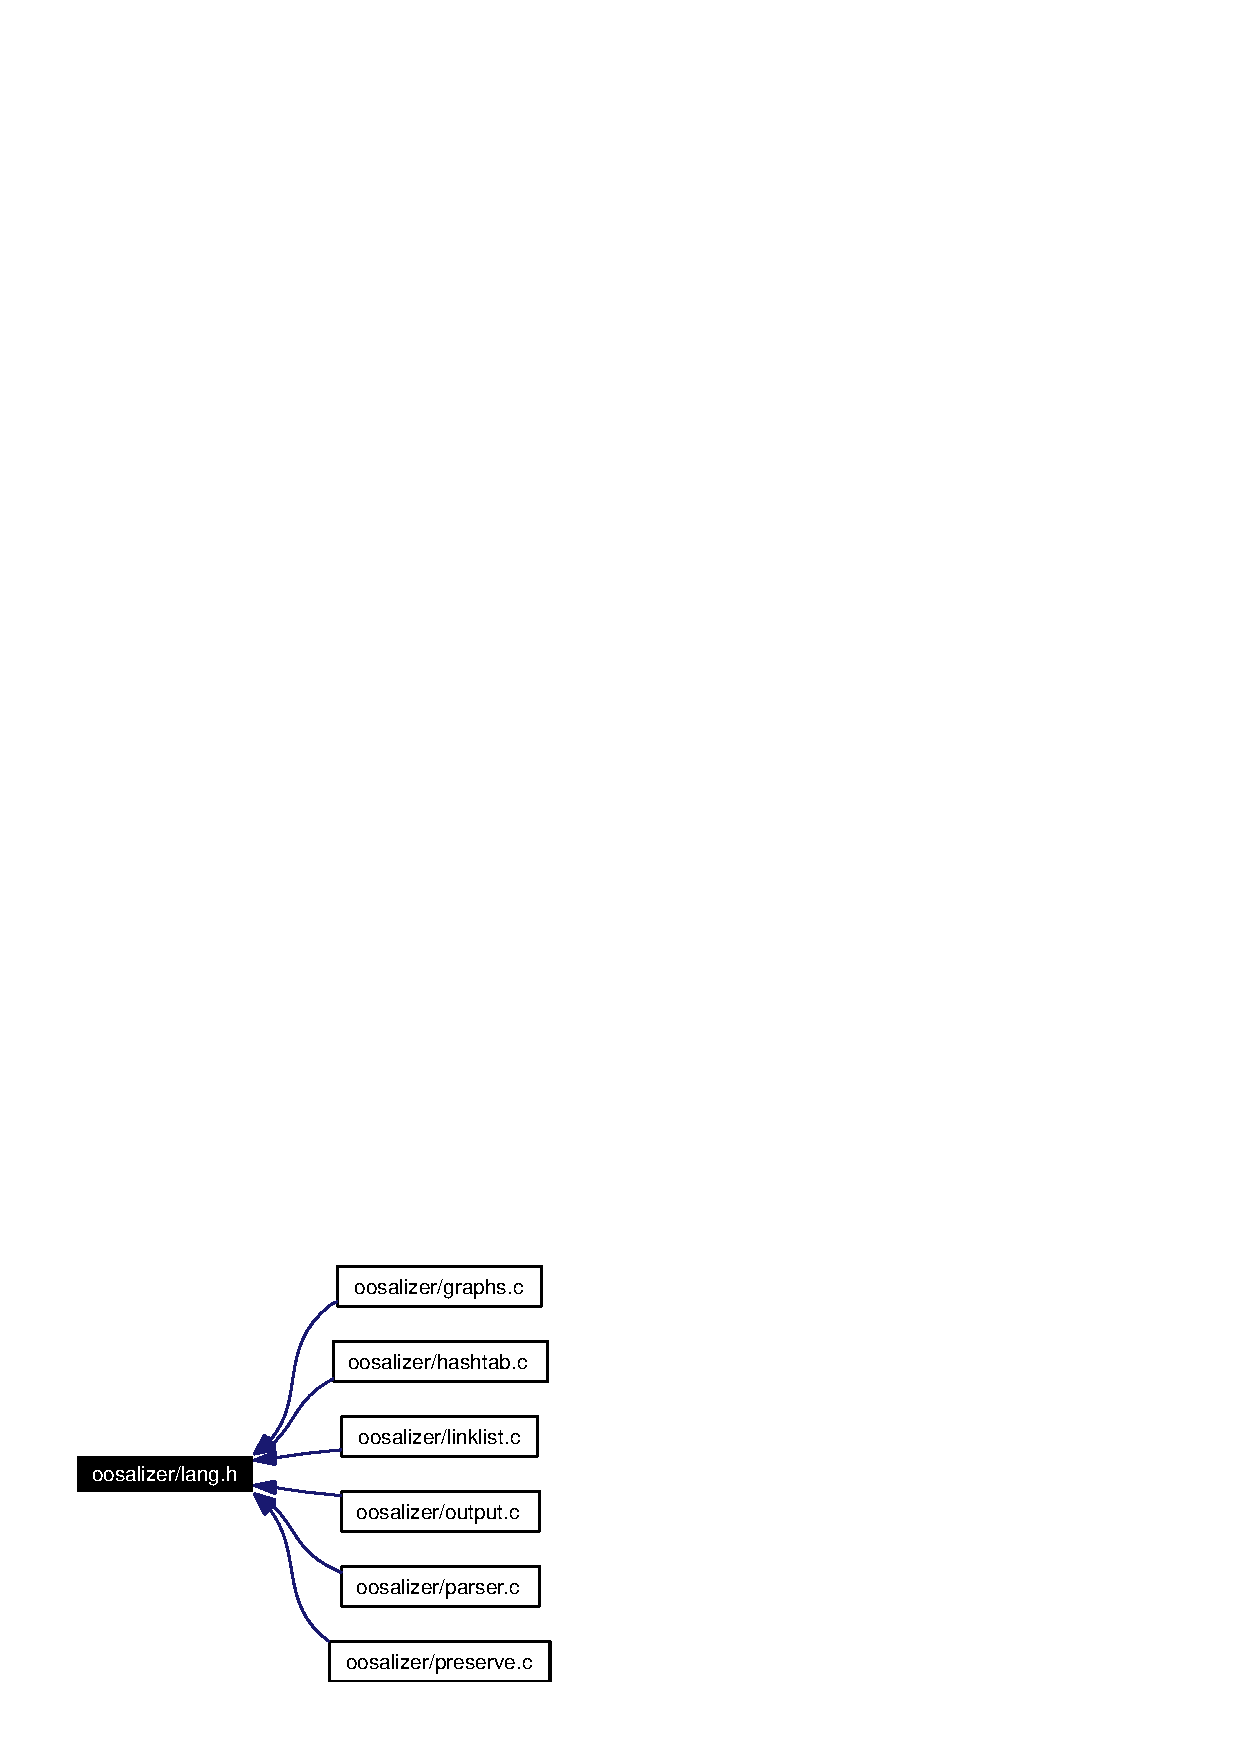
\includegraphics[width=132pt]{lang_8h__dep__incl}
\end{center}
\end{figure}
\subsection*{Variablen}
\begin{CompactItemize}
\item 
char $\ast$ {\bf language}
\item 
char $\ast$ {\bf msg\_\-records}
\item 
char $\ast$ {\bf msg\_\-addresses}
\item 
char $\ast$ {\bf msg\_\-ignored}
\item 
char $\ast$ {\bf msg\_\-bad}
\item 
char $\ast$ {\bf msg\_\-in}
\item 
char $\ast$ {\bf msg\_\-seconds}
\item 
char $\ast$ {\bf msg\_\-log\_\-err}
\item 
char $\ast$ {\bf msg\_\-log\_\-use}
\item 
char $\ast$ {\bf msg\_\-dir\_\-err}
\item 
char $\ast$ {\bf msg\_\-dir\_\-use}
\item 
char $\ast$ {\bf msg\_\-cur\_\-dir}
\item 
char $\ast$ {\bf msg\_\-hostname}
\item 
char $\ast$ {\bf msg\_\-ign\_\-hist}
\item 
char $\ast$ {\bf msg\_\-no\_\-hist}
\item 
char $\ast$ {\bf msg\_\-get\_\-hist}
\item 
char $\ast$ {\bf msg\_\-put\_\-hist}
\item 
char $\ast$ {\bf msg\_\-hist\_\-err}
\item 
char $\ast$ {\bf msg\_\-bad\_\-hist}
\item 
char $\ast$ {\bf msg\_\-bad\_\-conf}
\item 
char $\ast$ {\bf msg\_\-bad\_\-key}
\item 
char $\ast$ {\bf msg\_\-bad\_\-date}
\item 
char $\ast$ {\bf msg\_\-ign\_\-nscp}
\item 
char $\ast$ {\bf msg\_\-bad\_\-rec}
\item 
char $\ast$ {\bf msg\_\-no\_\-vrec}
\item 
char $\ast$ {\bf msg\_\-gen\_\-rpt}
\item 
char $\ast$ {\bf msg\_\-gen\_\-sum}
\item 
char $\ast$ {\bf msg\_\-get\_\-data}
\item 
char $\ast$ {\bf msg\_\-put\_\-data}
\item 
char $\ast$ {\bf msg\_\-no\_\-data}
\item 
char $\ast$ {\bf msg\_\-bad\_\-data}
\item 
char $\ast$ {\bf msg\_\-data\_\-err}
\item 
char $\ast$ {\bf msg\_\-dup\_\-data}
\item 
char $\ast$ {\bf msg\_\-dns\_\-nocf}
\item 
char $\ast$ {\bf msg\_\-dns\_\-nodb}
\item 
char $\ast$ {\bf msg\_\-dns\_\-nolk}
\item 
char $\ast$ {\bf msg\_\-dns\_\-usec}
\item 
char $\ast$ {\bf msg\_\-dns\_\-rslf}
\item 
char $\ast$ {\bf msg\_\-dns\_\-none}
\item 
char $\ast$ {\bf msg\_\-nomem\_\-ts}
\item 
char $\ast$ {\bf msg\_\-nomem\_\-tr}
\item 
char $\ast$ {\bf msg\_\-nomem\_\-tu}
\item 
char $\ast$ {\bf msg\_\-nomem\_\-tc}
\item 
char $\ast$ {\bf msg\_\-nomem\_\-ta}
\item 
char $\ast$ {\bf msg\_\-nomem\_\-tsr}
\item 
char $\ast$ {\bf msg\_\-nomem\_\-ti}
\item 
char $\ast$ {\bf msg\_\-nomem\_\-dh}
\item 
char $\ast$ {\bf msg\_\-nomem\_\-mh}
\item 
char $\ast$ {\bf msg\_\-nomem\_\-u}
\item 
char $\ast$ {\bf msg\_\-nomem\_\-a}
\item 
char $\ast$ {\bf msg\_\-nomem\_\-r}
\item 
char $\ast$ {\bf msg\_\-nomem\_\-sc}
\item 
char $\ast$ {\bf msg\_\-nomem\_\-i}
\item 
char $\ast$ {\bf msg\_\-big\_\-rec}
\item 
char $\ast$ {\bf msg\_\-big\_\-host}
\item 
char $\ast$ {\bf msg\_\-big\_\-date}
\item 
char $\ast$ {\bf msg\_\-big\_\-req}
\item 
char $\ast$ {\bf msg\_\-big\_\-ref}
\item 
char $\ast$ {\bf msg\_\-big\_\-user}
\item 
char $\ast$ {\bf msg\_\-big\_\-one}
\item 
char $\ast$ {\bf msg\_\-no\_\-open}
\item 
char $\ast$ {\bf h\_\-usage1}
\item 
char $\ast$ {\bf h\_\-usage2}
\item 
char $\ast$ {\bf h\_\-msg} [$\,$]
\item 
char $\ast$ {\bf msg\_\-hhdr\_\-sp}
\item 
char $\ast$ {\bf msg\_\-hhdr\_\-gt}
\item 
char $\ast$ {\bf msg\_\-main\_\-us}
\item 
char $\ast$ {\bf msg\_\-main\_\-per}
\item 
char $\ast$ {\bf msg\_\-main\_\-sum}
\item 
char $\ast$ {\bf msg\_\-main\_\-da}
\item 
char $\ast$ {\bf msg\_\-main\_\-mt}
\item 
char $\ast$ {\bf msg\_\-hmth\_\-du}
\item 
char $\ast$ {\bf msg\_\-hmth\_\-hu}
\item 
char $\ast$ {\bf msg\_\-h\_\-by}
\item 
char $\ast$ {\bf msg\_\-h\_\-avg}
\item 
char $\ast$ {\bf msg\_\-h\_\-max}
\item 
char $\ast$ {\bf msg\_\-h\_\-total}
\item 
char $\ast$ {\bf msg\_\-h\_\-totals}
\item 
char $\ast$ {\bf msg\_\-h\_\-day}
\item 
char $\ast$ {\bf msg\_\-h\_\-mth}
\item 
char $\ast$ {\bf msg\_\-h\_\-hour}
\item 
char $\ast$ {\bf msg\_\-h\_\-hits}
\item 
char $\ast$ {\bf msg\_\-h\_\-pages}
\item 
char $\ast$ {\bf msg\_\-h\_\-visits}
\item 
char $\ast$ {\bf msg\_\-h\_\-files}
\item 
char $\ast$ {\bf msg\_\-h\_\-sites}
\item 
char $\ast$ {\bf msg\_\-h\_\-xfer}
\item 
char $\ast$ {\bf msg\_\-h\_\-hname}
\item 
char $\ast$ {\bf msg\_\-h\_\-url}
\item 
char $\ast$ {\bf msg\_\-h\_\-agent}
\item 
char $\ast$ {\bf msg\_\-h\_\-ref}
\item 
char $\ast$ {\bf msg\_\-h\_\-ctry}
\item 
char $\ast$ {\bf msg\_\-h\_\-search}
\item 
char $\ast$ {\bf msg\_\-h\_\-uname}
\item 
char $\ast$ {\bf msg\_\-hlnk\_\-ds}
\item 
char $\ast$ {\bf msg\_\-hlnk\_\-hs}
\item 
char $\ast$ {\bf msg\_\-hlnk\_\-u}
\item 
char $\ast$ {\bf msg\_\-hlnk\_\-s}
\item 
char $\ast$ {\bf msg\_\-hlnk\_\-a}
\item 
char $\ast$ {\bf msg\_\-hlnk\_\-c}
\item 
char $\ast$ {\bf msg\_\-hlnk\_\-r}
\item 
char $\ast$ {\bf msg\_\-hlnk\_\-en}
\item 
char $\ast$ {\bf msg\_\-hlnk\_\-ex}
\item 
char $\ast$ {\bf msg\_\-hlnk\_\-sr}
\item 
char $\ast$ {\bf msg\_\-hlnk\_\-i}
\item 
char $\ast$ {\bf msg\_\-mtot\_\-ms}
\item 
char $\ast$ {\bf msg\_\-mtot\_\-th}
\item 
char $\ast$ {\bf msg\_\-mtot\_\-tf}
\item 
char $\ast$ {\bf msg\_\-mtot\_\-tx}
\item 
char $\ast$ {\bf msg\_\-mtot\_\-us}
\item 
char $\ast$ {\bf msg\_\-mtot\_\-ur}
\item 
char $\ast$ {\bf msg\_\-mtot\_\-ua}
\item 
char $\ast$ {\bf msg\_\-mtot\_\-uu}
\item 
char $\ast$ {\bf msg\_\-mtot\_\-ui}
\item 
char $\ast$ {\bf msg\_\-mtot\_\-mhd}
\item 
char $\ast$ {\bf msg\_\-mtot\_\-mhh}
\item 
char $\ast$ {\bf msg\_\-mtot\_\-mfd}
\item 
char $\ast$ {\bf msg\_\-mtot\_\-mpd}
\item 
char $\ast$ {\bf msg\_\-mtot\_\-mvd}
\item 
char $\ast$ {\bf msg\_\-mtot\_\-mkd}
\item 
char $\ast$ {\bf msg\_\-mtot\_\-rc}
\item 
char $\ast$ {\bf msg\_\-dtot\_\-ds}
\item 
char $\ast$ {\bf msg\_\-htot\_\-hs}
\item 
char $\ast$ {\bf msg\_\-ctry\_\-use}
\item 
char $\ast$ {\bf msg\_\-top\_\-top}
\item 
char $\ast$ {\bf msg\_\-top\_\-of}
\item 
char $\ast$ {\bf msg\_\-top\_\-s}
\item 
char $\ast$ {\bf msg\_\-top\_\-u}
\item 
char $\ast$ {\bf msg\_\-top\_\-r}
\item 
char $\ast$ {\bf msg\_\-top\_\-a}
\item 
char $\ast$ {\bf msg\_\-top\_\-c}
\item 
char $\ast$ {\bf msg\_\-top\_\-en}
\item 
char $\ast$ {\bf msg\_\-top\_\-ex}
\item 
char $\ast$ {\bf msg\_\-top\_\-sr}
\item 
char $\ast$ {\bf msg\_\-top\_\-i}
\item 
char $\ast$ {\bf msg\_\-v\_\-sites}
\item 
char $\ast$ {\bf msg\_\-v\_\-urls}
\item 
char $\ast$ {\bf msg\_\-v\_\-refs}
\item 
char $\ast$ {\bf msg\_\-v\_\-agents}
\item 
char $\ast$ {\bf msg\_\-v\_\-search}
\item 
char $\ast$ {\bf msg\_\-v\_\-users}
\item 
char $\ast$ {\bf msg\_\-title}
\item 
char $\ast$ {\bf msg\_\-h\_\-other}
\item 
char $\ast$ {\bf s\_\-month} [12]
\item 
char $\ast$ {\bf l\_\-month} [12]
\item 
{\bf response\_\-code} {\bf response} [$\,$]
\item 
{\bf country\_\-code} {\bf ctry} [$\,$]
\end{CompactItemize}


\subsection{Variablen-Dokumentation}
\index{lang.h@{lang.h}!ctry@{ctry}}
\index{ctry@{ctry}!lang.h@{lang.h}}
\subsubsection{\setlength{\rightskip}{0pt plus 5cm}struct {\bf country\_\-code} {\bf ctry}[$\,$]}\label{lang_8h_2da4e4ffd517ae749587bd8692434663}




Wird benutzt von main() und top\_\-ctry\_\-table().\index{lang.h@{lang.h}!h_msg@{h\_\-msg}}
\index{h_msg@{h\_\-msg}!lang.h@{lang.h}}
\subsubsection{\setlength{\rightskip}{0pt plus 5cm}char$\ast$ {\bf h\_\-msg}[$\,$]}\label{lang_8h_b5b6cedf99598af62b8cd4bc308493b4}




Wird benutzt von print\_\-opts().\index{lang.h@{lang.h}!h_usage1@{h\_\-usage1}}
\index{h_usage1@{h\_\-usage1}!lang.h@{lang.h}}
\subsubsection{\setlength{\rightskip}{0pt plus 5cm}char$\ast$ {\bf h\_\-usage1}}\label{lang_8h_9ba617b9ad4b243163879779992cb922}




Wird benutzt von print\_\-opts().\index{lang.h@{lang.h}!h_usage2@{h\_\-usage2}}
\index{h_usage2@{h\_\-usage2}!lang.h@{lang.h}}
\subsubsection{\setlength{\rightskip}{0pt plus 5cm}char$\ast$ {\bf h\_\-usage2}}\label{lang_8h_3b3adac04f9e05f7ff5b592fcf18cdc6}




Wird benutzt von print\_\-opts().\index{lang.h@{lang.h}!l_month@{l\_\-month}}
\index{l_month@{l\_\-month}!lang.h@{lang.h}}
\subsubsection{\setlength{\rightskip}{0pt plus 5cm}char$\ast$ {\bf l\_\-month}[12]}\label{lang_8h_e75828f9450cccbb02d410d60a6caa1d}




Wird benutzt von all\_\-agents\_\-page(), all\_\-refs\_\-page(), all\_\-search\_\-page(), all\_\-sites\_\-page(), all\_\-urls\_\-page(), all\_\-users\_\-page(), daily\_\-total\_\-table(), hourly\_\-total\_\-table() und write\_\-month\_\-html().\index{lang.h@{lang.h}!language@{language}}
\index{language@{language}!lang.h@{lang.h}}
\subsubsection{\setlength{\rightskip}{0pt plus 5cm}char$\ast$ {\bf language}}\label{lang_8h_8ae4b47621b125e915cee8ccdaa2095c}




Wird benutzt von print\_\-version().\index{lang.h@{lang.h}!msg_addresses@{msg\_\-addresses}}
\index{msg_addresses@{msg\_\-addresses}!lang.h@{lang.h}}
\subsubsection{\setlength{\rightskip}{0pt plus 5cm}char$\ast$ {\bf msg\_\-addresses}}\label{lang_8h_61f6c7ec6657cd88a32549b14d43d489}


\index{lang.h@{lang.h}!msg_bad@{msg\_\-bad}}
\index{msg_bad@{msg\_\-bad}!lang.h@{lang.h}}
\subsubsection{\setlength{\rightskip}{0pt plus 5cm}char$\ast$ {\bf msg\_\-bad}}\label{lang_8h_d0f59bbd0fcb26d5e153ffc4c1a907f8}


\index{lang.h@{lang.h}!msg_bad_conf@{msg\_\-bad\_\-conf}}
\index{msg_bad_conf@{msg\_\-bad\_\-conf}!lang.h@{lang.h}}
\subsubsection{\setlength{\rightskip}{0pt plus 5cm}char$\ast$ {\bf msg\_\-bad\_\-conf}}\label{lang_8h_c96834cc1626aa91d6edfb4f59e3a742}




Wird benutzt von get\_\-config().\index{lang.h@{lang.h}!msg_bad_data@{msg\_\-bad\_\-data}}
\index{msg_bad_data@{msg\_\-bad\_\-data}!lang.h@{lang.h}}
\subsubsection{\setlength{\rightskip}{0pt plus 5cm}char$\ast$ {\bf msg\_\-bad\_\-data}}\label{lang_8h_8e438fc75d1860600b450deead48c385}


\index{lang.h@{lang.h}!msg_bad_date@{msg\_\-bad\_\-date}}
\index{msg_bad_date@{msg\_\-bad\_\-date}!lang.h@{lang.h}}
\subsubsection{\setlength{\rightskip}{0pt plus 5cm}char$\ast$ {\bf msg\_\-bad\_\-date}}\label{lang_8h_fa5fa3fc2684b89b20a57f5081e6cfe1}


\index{lang.h@{lang.h}!msg_bad_hist@{msg\_\-bad\_\-hist}}
\index{msg_bad_hist@{msg\_\-bad\_\-hist}!lang.h@{lang.h}}
\subsubsection{\setlength{\rightskip}{0pt plus 5cm}char$\ast$ {\bf msg\_\-bad\_\-hist}}\label{lang_8h_41d93d2d187e1c3836391e695f8344a7}


\index{lang.h@{lang.h}!msg_bad_key@{msg\_\-bad\_\-key}}
\index{msg_bad_key@{msg\_\-bad\_\-key}!lang.h@{lang.h}}
\subsubsection{\setlength{\rightskip}{0pt plus 5cm}char$\ast$ {\bf msg\_\-bad\_\-key}}\label{lang_8h_677f59db55311afd2a3a860c1e36e004}




Wird benutzt von get\_\-config().\index{lang.h@{lang.h}!msg_bad_rec@{msg\_\-bad\_\-rec}}
\index{msg_bad_rec@{msg\_\-bad\_\-rec}!lang.h@{lang.h}}
\subsubsection{\setlength{\rightskip}{0pt plus 5cm}char$\ast$ {\bf msg\_\-bad\_\-rec}}\label{lang_8h_bc0778be3e6f0173eda81a2a70e97fee}


\index{lang.h@{lang.h}!msg_big_date@{msg\_\-big\_\-date}}
\index{msg_big_date@{msg\_\-big\_\-date}!lang.h@{lang.h}}
\subsubsection{\setlength{\rightskip}{0pt plus 5cm}char$\ast$ {\bf msg\_\-big\_\-date}}\label{lang_8h_5cf2461dfbe62c32f225953b0326462c}




Wird benutzt von parse\_\-record\_\-web().\index{lang.h@{lang.h}!msg_big_host@{msg\_\-big\_\-host}}
\index{msg_big_host@{msg\_\-big\_\-host}!lang.h@{lang.h}}
\subsubsection{\setlength{\rightskip}{0pt plus 5cm}char$\ast$ {\bf msg\_\-big\_\-host}}\label{lang_8h_6ce7f8ad0ab920f3113dff9e936dc9a5}




Wird benutzt von parse\_\-record\_\-squid() und parse\_\-record\_\-web().\index{lang.h@{lang.h}!msg_big_one@{msg\_\-big\_\-one}}
\index{msg_big_one@{msg\_\-big\_\-one}!lang.h@{lang.h}}
\subsubsection{\setlength{\rightskip}{0pt plus 5cm}char$\ast$ {\bf msg\_\-big\_\-one}}\label{lang_8h_a2ee47975118e6f57ce4a10d1baeef26}




Wird benutzt von new\_\-anode(), new\_\-glist(), new\_\-hnode(), new\_\-inode(), new\_\-nlist(), new\_\-rnode(), new\_\-snode() und new\_\-unode().\index{lang.h@{lang.h}!msg_big_rec@{msg\_\-big\_\-rec}}
\index{msg_big_rec@{msg\_\-big\_\-rec}!lang.h@{lang.h}}
\subsubsection{\setlength{\rightskip}{0pt plus 5cm}char$\ast$ {\bf msg\_\-big\_\-rec}}\label{lang_8h_1ef9a73473db9b45b770351a8c69ff33}


\index{lang.h@{lang.h}!msg_big_ref@{msg\_\-big\_\-ref}}
\index{msg_big_ref@{msg\_\-big\_\-ref}!lang.h@{lang.h}}
\subsubsection{\setlength{\rightskip}{0pt plus 5cm}char$\ast$ {\bf msg\_\-big\_\-ref}}\label{lang_8h_ae731a9fc075ed277c6ee4b8a6384ea0}




Wird benutzt von parse\_\-record\_\-web().\index{lang.h@{lang.h}!msg_big_req@{msg\_\-big\_\-req}}
\index{msg_big_req@{msg\_\-big\_\-req}!lang.h@{lang.h}}
\subsubsection{\setlength{\rightskip}{0pt plus 5cm}char$\ast$ {\bf msg\_\-big\_\-req}}\label{lang_8h_43eab59f53dc27f4f768755b759684f7}




Wird benutzt von parse\_\-record\_\-squid() und parse\_\-record\_\-web().\index{lang.h@{lang.h}!msg_big_user@{msg\_\-big\_\-user}}
\index{msg_big_user@{msg\_\-big\_\-user}!lang.h@{lang.h}}
\subsubsection{\setlength{\rightskip}{0pt plus 5cm}char$\ast$ {\bf msg\_\-big\_\-user}}\label{lang_8h_9f2cc97f2917013977b0b0969a5c7960}




Wird benutzt von parse\_\-record\_\-web().\index{lang.h@{lang.h}!msg_ctry_use@{msg\_\-ctry\_\-use}}
\index{msg_ctry_use@{msg\_\-ctry\_\-use}!lang.h@{lang.h}}
\subsubsection{\setlength{\rightskip}{0pt plus 5cm}char$\ast$ {\bf msg\_\-ctry\_\-use}}\label{lang_8h_d86bfd951b9d1f489e0fac664d76643e}


\index{lang.h@{lang.h}!msg_cur_dir@{msg\_\-cur\_\-dir}}
\index{msg_cur_dir@{msg\_\-cur\_\-dir}!lang.h@{lang.h}}
\subsubsection{\setlength{\rightskip}{0pt plus 5cm}char$\ast$ {\bf msg\_\-cur\_\-dir}}\label{lang_8h_753780d6a71f07ea59ad96c3b4425d3f}


\index{lang.h@{lang.h}!msg_data_err@{msg\_\-data\_\-err}}
\index{msg_data_err@{msg\_\-data\_\-err}!lang.h@{lang.h}}
\subsubsection{\setlength{\rightskip}{0pt plus 5cm}char$\ast$ {\bf msg\_\-data\_\-err}}\label{lang_8h_d78d59d0e6763c1c3eee300b87985f85}


\index{lang.h@{lang.h}!msg_dir_err@{msg\_\-dir\_\-err}}
\index{msg_dir_err@{msg\_\-dir\_\-err}!lang.h@{lang.h}}
\subsubsection{\setlength{\rightskip}{0pt plus 5cm}char$\ast$ {\bf msg\_\-dir\_\-err}}\label{lang_8h_38a10d8fc0f51c7a330c6fb6d6e471de}


\index{lang.h@{lang.h}!msg_dir_use@{msg\_\-dir\_\-use}}
\index{msg_dir_use@{msg\_\-dir\_\-use}!lang.h@{lang.h}}
\subsubsection{\setlength{\rightskip}{0pt plus 5cm}char$\ast$ {\bf msg\_\-dir\_\-use}}\label{lang_8h_dd2c26fd0af447d6b6b6aad63715299a}


\index{lang.h@{lang.h}!msg_dns_nocf@{msg\_\-dns\_\-nocf}}
\index{msg_dns_nocf@{msg\_\-dns\_\-nocf}!lang.h@{lang.h}}
\subsubsection{\setlength{\rightskip}{0pt plus 5cm}char$\ast$ {\bf msg\_\-dns\_\-nocf}}\label{lang_8h_e1ba4137910c0624529a95d485160da8}


\index{lang.h@{lang.h}!msg_dns_nodb@{msg\_\-dns\_\-nodb}}
\index{msg_dns_nodb@{msg\_\-dns\_\-nodb}!lang.h@{lang.h}}
\subsubsection{\setlength{\rightskip}{0pt plus 5cm}char$\ast$ {\bf msg\_\-dns\_\-nodb}}\label{lang_8h_76e75b9036f799fbd887d7a3222e01ca}


\index{lang.h@{lang.h}!msg_dns_nolk@{msg\_\-dns\_\-nolk}}
\index{msg_dns_nolk@{msg\_\-dns\_\-nolk}!lang.h@{lang.h}}
\subsubsection{\setlength{\rightskip}{0pt plus 5cm}char$\ast$ {\bf msg\_\-dns\_\-nolk}}\label{lang_8h_a488fc78d64f1c5208d73d133d089452}


\index{lang.h@{lang.h}!msg_dns_none@{msg\_\-dns\_\-none}}
\index{msg_dns_none@{msg\_\-dns\_\-none}!lang.h@{lang.h}}
\subsubsection{\setlength{\rightskip}{0pt plus 5cm}char$\ast$ {\bf msg\_\-dns\_\-none}}\label{lang_8h_9f52d036b0b7b7550e759af41428d725}


\index{lang.h@{lang.h}!msg_dns_rslf@{msg\_\-dns\_\-rslf}}
\index{msg_dns_rslf@{msg\_\-dns\_\-rslf}!lang.h@{lang.h}}
\subsubsection{\setlength{\rightskip}{0pt plus 5cm}char$\ast$ {\bf msg\_\-dns\_\-rslf}}\label{lang_8h_2b21e7d80cef6c8ac7f7ad94a56e2dc6}


\index{lang.h@{lang.h}!msg_dns_usec@{msg\_\-dns\_\-usec}}
\index{msg_dns_usec@{msg\_\-dns\_\-usec}!lang.h@{lang.h}}
\subsubsection{\setlength{\rightskip}{0pt plus 5cm}char$\ast$ {\bf msg\_\-dns\_\-usec}}\label{lang_8h_b73f8c1a203f27cb555899a882beed0a}


\index{lang.h@{lang.h}!msg_dtot_ds@{msg\_\-dtot\_\-ds}}
\index{msg_dtot_ds@{msg\_\-dtot\_\-ds}!lang.h@{lang.h}}
\subsubsection{\setlength{\rightskip}{0pt plus 5cm}char$\ast$ {\bf msg\_\-dtot\_\-ds}}\label{lang_8h_05ed4ddbb649bb7506fc41d1607127ae}




Wird benutzt von daily\_\-total\_\-table().\index{lang.h@{lang.h}!msg_dup_data@{msg\_\-dup\_\-data}}
\index{msg_dup_data@{msg\_\-dup\_\-data}!lang.h@{lang.h}}
\subsubsection{\setlength{\rightskip}{0pt plus 5cm}char$\ast$ {\bf msg\_\-dup\_\-data}}\label{lang_8h_5dc0ad29f3bcca57145a156d92c331c2}


\index{lang.h@{lang.h}!msg_gen_rpt@{msg\_\-gen\_\-rpt}}
\index{msg_gen_rpt@{msg\_\-gen\_\-rpt}!lang.h@{lang.h}}
\subsubsection{\setlength{\rightskip}{0pt plus 5cm}char$\ast$ {\bf msg\_\-gen\_\-rpt}}\label{lang_8h_5e34eccd1e2035aea1b7159063d915f8}




Wird benutzt von write\_\-month\_\-html().\index{lang.h@{lang.h}!msg_gen_sum@{msg\_\-gen\_\-sum}}
\index{msg_gen_sum@{msg\_\-gen\_\-sum}!lang.h@{lang.h}}
\subsubsection{\setlength{\rightskip}{0pt plus 5cm}char$\ast$ {\bf msg\_\-gen\_\-sum}}\label{lang_8h_6e6be76001566785c2bcfcbab6dbca41}




Wird benutzt von write\_\-main\_\-index().\index{lang.h@{lang.h}!msg_get_data@{msg\_\-get\_\-data}}
\index{msg_get_data@{msg\_\-get\_\-data}!lang.h@{lang.h}}
\subsubsection{\setlength{\rightskip}{0pt plus 5cm}char$\ast$ {\bf msg\_\-get\_\-data}}\label{lang_8h_2911108863867222d664581ddfa69db0}




Wird benutzt von restore\_\-state().\index{lang.h@{lang.h}!msg_get_hist@{msg\_\-get\_\-hist}}
\index{msg_get_hist@{msg\_\-get\_\-hist}!lang.h@{lang.h}}
\subsubsection{\setlength{\rightskip}{0pt plus 5cm}char$\ast$ {\bf msg\_\-get\_\-hist}}\label{lang_8h_13a7e44b057b2a3dfe84864e6e955313}


\index{lang.h@{lang.h}!msg_h_agent@{msg\_\-h\_\-agent}}
\index{msg_h_agent@{msg\_\-h\_\-agent}!lang.h@{lang.h}}
\subsubsection{\setlength{\rightskip}{0pt plus 5cm}char$\ast$ {\bf msg\_\-h\_\-agent}}\label{lang_8h_88ef492f810cce55301b0422c8c135ec}




Wird benutzt von all\_\-agents\_\-page(), dump\_\-all\_\-agents() und top\_\-agents\_\-table().\index{lang.h@{lang.h}!msg_h_avg@{msg\_\-h\_\-avg}}
\index{msg_h_avg@{msg\_\-h\_\-avg}!lang.h@{lang.h}}
\subsubsection{\setlength{\rightskip}{0pt plus 5cm}char$\ast$ {\bf msg\_\-h\_\-avg}}\label{lang_8h_41aae7d7f619d71ff5b47f541d3c8dfd}




Wird benutzt von hourly\_\-total\_\-table().\index{lang.h@{lang.h}!msg_h_by@{msg\_\-h\_\-by}}
\index{msg_h_by@{msg\_\-h\_\-by}!lang.h@{lang.h}}
\subsubsection{\setlength{\rightskip}{0pt plus 5cm}char$\ast$ {\bf msg\_\-h\_\-by}}\label{lang_8h_445f2712cd567c8d33b7fb797843dea0}




Wird benutzt von top\_\-sites\_\-table() und top\_\-urls\_\-table().\index{lang.h@{lang.h}!msg_h_ctry@{msg\_\-h\_\-ctry}}
\index{msg_h_ctry@{msg\_\-h\_\-ctry}!lang.h@{lang.h}}
\subsubsection{\setlength{\rightskip}{0pt plus 5cm}char$\ast$ {\bf msg\_\-h\_\-ctry}}\label{lang_8h_3d13e2f231a2e408c85d587974fab840}


\index{lang.h@{lang.h}!msg_h_day@{msg\_\-h\_\-day}}
\index{msg_h_day@{msg\_\-h\_\-day}!lang.h@{lang.h}}
\subsubsection{\setlength{\rightskip}{0pt plus 5cm}char$\ast$ {\bf msg\_\-h\_\-day}}\label{lang_8h_4ea7eb5797dae19227edd460213b7b0a}




Wird benutzt von daily\_\-total\_\-table().\index{lang.h@{lang.h}!msg_h_files@{msg\_\-h\_\-files}}
\index{msg_h_files@{msg\_\-h\_\-files}!lang.h@{lang.h}}
\subsubsection{\setlength{\rightskip}{0pt plus 5cm}char$\ast$ {\bf msg\_\-h\_\-files}}\label{lang_8h_17cdd1238613c58645be27ec86da138c}




Wird benutzt von all\_\-sites\_\-page(), all\_\-users\_\-page(), daily\_\-total\_\-table(), dump\_\-all\_\-sites(), dump\_\-all\_\-users(), hourly\_\-total\_\-table(), top\_\-sites\_\-table() und top\_\-users\_\-table().\index{lang.h@{lang.h}!msg_h_hits@{msg\_\-h\_\-hits}}
\index{msg_h_hits@{msg\_\-h\_\-hits}!lang.h@{lang.h}}
\subsubsection{\setlength{\rightskip}{0pt plus 5cm}char$\ast$ {\bf msg\_\-h\_\-hits}}\label{lang_8h_529f40f7939bbf363a37235b1b209b62}




Wird benutzt von all\_\-agents\_\-page(), all\_\-refs\_\-page(), all\_\-search\_\-page(), all\_\-sites\_\-page(), all\_\-urls\_\-page(), all\_\-users\_\-page(), daily\_\-total\_\-table(), dump\_\-all\_\-agents(), dump\_\-all\_\-refs(), dump\_\-all\_\-search(), dump\_\-all\_\-sites(), dump\_\-all\_\-urls(), dump\_\-all\_\-users(), hourly\_\-total\_\-table(), top\_\-agents\_\-table(), top\_\-entry\_\-table(), top\_\-refs\_\-table(), top\_\-search\_\-table(), top\_\-sites\_\-table(), top\_\-urls\_\-table() und top\_\-users\_\-table().\index{lang.h@{lang.h}!msg_h_hname@{msg\_\-h\_\-hname}}
\index{msg_h_hname@{msg\_\-h\_\-hname}!lang.h@{lang.h}}
\subsubsection{\setlength{\rightskip}{0pt plus 5cm}char$\ast$ {\bf msg\_\-h\_\-hname}}\label{lang_8h_389648e11c07ae97a6c19e049401a01f}




Wird benutzt von all\_\-sites\_\-page(), dump\_\-all\_\-sites() und top\_\-sites\_\-table().\index{lang.h@{lang.h}!msg_h_hour@{msg\_\-h\_\-hour}}
\index{msg_h_hour@{msg\_\-h\_\-hour}!lang.h@{lang.h}}
\subsubsection{\setlength{\rightskip}{0pt plus 5cm}char$\ast$ {\bf msg\_\-h\_\-hour}}\label{lang_8h_75d18a9846e48af78b39df85c88b425e}




Wird benutzt von hourly\_\-total\_\-table().\index{lang.h@{lang.h}!msg_h_max@{msg\_\-h\_\-max}}
\index{msg_h_max@{msg\_\-h\_\-max}!lang.h@{lang.h}}
\subsubsection{\setlength{\rightskip}{0pt plus 5cm}char$\ast$ {\bf msg\_\-h\_\-max}}\label{lang_8h_081ce53502d2128996c22bef5bd24a53}


\index{lang.h@{lang.h}!msg_h_mth@{msg\_\-h\_\-mth}}
\index{msg_h_mth@{msg\_\-h\_\-mth}!lang.h@{lang.h}}
\subsubsection{\setlength{\rightskip}{0pt plus 5cm}char$\ast$ {\bf msg\_\-h\_\-mth}}\label{lang_8h_3f7e8b2df4f2e24306b823798e8ee780}


\index{lang.h@{lang.h}!msg_h_other@{msg\_\-h\_\-other}}
\index{msg_h_other@{msg\_\-h\_\-other}!lang.h@{lang.h}}
\subsubsection{\setlength{\rightskip}{0pt plus 5cm}char$\ast$ {\bf msg\_\-h\_\-other}}\label{lang_8h_b351e925c0e7fcdb3483ab94cba23c9c}


\index{lang.h@{lang.h}!msg_h_pages@{msg\_\-h\_\-pages}}
\index{msg_h_pages@{msg\_\-h\_\-pages}!lang.h@{lang.h}}
\subsubsection{\setlength{\rightskip}{0pt plus 5cm}char$\ast$ {\bf msg\_\-h\_\-pages}}\label{lang_8h_db4c9ee2d878d68d50a008b354042927}




Wird benutzt von daily\_\-total\_\-table() und hourly\_\-total\_\-table().\index{lang.h@{lang.h}!msg_h_ref@{msg\_\-h\_\-ref}}
\index{msg_h_ref@{msg\_\-h\_\-ref}!lang.h@{lang.h}}
\subsubsection{\setlength{\rightskip}{0pt plus 5cm}char$\ast$ {\bf msg\_\-h\_\-ref}}\label{lang_8h_044f17c6b922b4c62fcd9d60dc5743b6}




Wird benutzt von all\_\-refs\_\-page(), dump\_\-all\_\-refs() und top\_\-refs\_\-table().\index{lang.h@{lang.h}!msg_h_search@{msg\_\-h\_\-search}}
\index{msg_h_search@{msg\_\-h\_\-search}!lang.h@{lang.h}}
\subsubsection{\setlength{\rightskip}{0pt plus 5cm}char$\ast$ {\bf msg\_\-h\_\-search}}\label{lang_8h_a60f1bd74d1fb88de31964981fc8d0d6}




Wird benutzt von all\_\-search\_\-page(), dump\_\-all\_\-search() und top\_\-search\_\-table().\index{lang.h@{lang.h}!msg_h_sites@{msg\_\-h\_\-sites}}
\index{msg_h_sites@{msg\_\-h\_\-sites}!lang.h@{lang.h}}
\subsubsection{\setlength{\rightskip}{0pt plus 5cm}char$\ast$ {\bf msg\_\-h\_\-sites}}\label{lang_8h_40421f6c86f03b581ec81e010c8d0086}




Wird benutzt von all\_\-sites\_\-page() und daily\_\-total\_\-table().\index{lang.h@{lang.h}!msg_h_total@{msg\_\-h\_\-total}}
\index{msg_h_total@{msg\_\-h\_\-total}!lang.h@{lang.h}}
\subsubsection{\setlength{\rightskip}{0pt plus 5cm}char$\ast$ {\bf msg\_\-h\_\-total}}\label{lang_8h_55b57954b9d1fe93bc7ddd126a839db0}




Wird benutzt von hourly\_\-total\_\-table().\index{lang.h@{lang.h}!msg_h_totals@{msg\_\-h\_\-totals}}
\index{msg_h_totals@{msg\_\-h\_\-totals}!lang.h@{lang.h}}
\subsubsection{\setlength{\rightskip}{0pt plus 5cm}char$\ast$ {\bf msg\_\-h\_\-totals}}\label{lang_8h_dafe58551b800a16ddc8b3111529262f}


\index{lang.h@{lang.h}!msg_h_uname@{msg\_\-h\_\-uname}}
\index{msg_h_uname@{msg\_\-h\_\-uname}!lang.h@{lang.h}}
\subsubsection{\setlength{\rightskip}{0pt plus 5cm}char$\ast$ {\bf msg\_\-h\_\-uname}}\label{lang_8h_04b9008a2c6d6752de424ad84772f803}




Wird benutzt von all\_\-users\_\-page(), dump\_\-all\_\-users() und top\_\-users\_\-table().\index{lang.h@{lang.h}!msg_h_url@{msg\_\-h\_\-url}}
\index{msg_h_url@{msg\_\-h\_\-url}!lang.h@{lang.h}}
\subsubsection{\setlength{\rightskip}{0pt plus 5cm}char$\ast$ {\bf msg\_\-h\_\-url}}\label{lang_8h_c2422ae6f0a2e8bdc0caa4fc75645f4b}




Wird benutzt von all\_\-urls\_\-page(), dump\_\-all\_\-urls(), top\_\-entry\_\-table() und top\_\-urls\_\-table().\index{lang.h@{lang.h}!msg_h_visits@{msg\_\-h\_\-visits}}
\index{msg_h_visits@{msg\_\-h\_\-visits}!lang.h@{lang.h}}
\subsubsection{\setlength{\rightskip}{0pt plus 5cm}char$\ast$ {\bf msg\_\-h\_\-visits}}\label{lang_8h_daf199b209b9dd7996804b6018b8539f}




Wird benutzt von all\_\-sites\_\-page(), all\_\-users\_\-page(), daily\_\-total\_\-table(), dump\_\-all\_\-sites(), dump\_\-all\_\-users(), top\_\-entry\_\-table(), top\_\-sites\_\-table() und top\_\-users\_\-table().\index{lang.h@{lang.h}!msg_h_xfer@{msg\_\-h\_\-xfer}}
\index{msg_h_xfer@{msg\_\-h\_\-xfer}!lang.h@{lang.h}}
\subsubsection{\setlength{\rightskip}{0pt plus 5cm}char$\ast$ {\bf msg\_\-h\_\-xfer}}\label{lang_8h_b193be580f6d1d61bb87dfb4e9f8547c}




Wird benutzt von all\_\-sites\_\-page(), all\_\-urls\_\-page(), all\_\-users\_\-page(), daily\_\-total\_\-table(), dump\_\-all\_\-sites(), dump\_\-all\_\-urls(), dump\_\-all\_\-users(), hourly\_\-total\_\-table(), top\_\-sites\_\-table(), top\_\-urls\_\-table() und top\_\-users\_\-table().\index{lang.h@{lang.h}!msg_hhdr_gt@{msg\_\-hhdr\_\-gt}}
\index{msg_hhdr_gt@{msg\_\-hhdr\_\-gt}!lang.h@{lang.h}}
\subsubsection{\setlength{\rightskip}{0pt plus 5cm}char$\ast$ {\bf msg\_\-hhdr\_\-gt}}\label{lang_8h_2b9f2f69e665448e249b8ce01055196e}




Wird benutzt von write\_\-html\_\-head().\index{lang.h@{lang.h}!msg_hhdr_sp@{msg\_\-hhdr\_\-sp}}
\index{msg_hhdr_sp@{msg\_\-hhdr\_\-sp}!lang.h@{lang.h}}
\subsubsection{\setlength{\rightskip}{0pt plus 5cm}char$\ast$ {\bf msg\_\-hhdr\_\-sp}}\label{lang_8h_3d3b7751d6e494d468adb748ca65167c}




Wird benutzt von write\_\-html\_\-head().\index{lang.h@{lang.h}!msg_hist_err@{msg\_\-hist\_\-err}}
\index{msg_hist_err@{msg\_\-hist\_\-err}!lang.h@{lang.h}}
\subsubsection{\setlength{\rightskip}{0pt plus 5cm}char$\ast$ {\bf msg\_\-hist\_\-err}}\label{lang_8h_78b4e52380a3d91b131c074eea130b82}


\index{lang.h@{lang.h}!msg_hlnk_a@{msg\_\-hlnk\_\-a}}
\index{msg_hlnk_a@{msg\_\-hlnk\_\-a}!lang.h@{lang.h}}
\subsubsection{\setlength{\rightskip}{0pt plus 5cm}char$\ast$ {\bf msg\_\-hlnk\_\-a}}\label{lang_8h_63bc4c24fa58aadfe6b07847a5385727}




Wird benutzt von month\_\-links().\index{lang.h@{lang.h}!msg_hlnk_c@{msg\_\-hlnk\_\-c}}
\index{msg_hlnk_c@{msg\_\-hlnk\_\-c}!lang.h@{lang.h}}
\subsubsection{\setlength{\rightskip}{0pt plus 5cm}char$\ast$ {\bf msg\_\-hlnk\_\-c}}\label{lang_8h_db006844c6196bd298ae047e146032c6}




Wird benutzt von month\_\-links().\index{lang.h@{lang.h}!msg_hlnk_ds@{msg\_\-hlnk\_\-ds}}
\index{msg_hlnk_ds@{msg\_\-hlnk\_\-ds}!lang.h@{lang.h}}
\subsubsection{\setlength{\rightskip}{0pt plus 5cm}char$\ast$ {\bf msg\_\-hlnk\_\-ds}}\label{lang_8h_f477d45ee4c0a42dd8e2badd00583eb3}




Wird benutzt von month\_\-links().\index{lang.h@{lang.h}!msg_hlnk_en@{msg\_\-hlnk\_\-en}}
\index{msg_hlnk_en@{msg\_\-hlnk\_\-en}!lang.h@{lang.h}}
\subsubsection{\setlength{\rightskip}{0pt plus 5cm}char$\ast$ {\bf msg\_\-hlnk\_\-en}}\label{lang_8h_cfa5f6db28bff540ecfe2ee1f05323c2}




Wird benutzt von month\_\-links().\index{lang.h@{lang.h}!msg_hlnk_ex@{msg\_\-hlnk\_\-ex}}
\index{msg_hlnk_ex@{msg\_\-hlnk\_\-ex}!lang.h@{lang.h}}
\subsubsection{\setlength{\rightskip}{0pt plus 5cm}char$\ast$ {\bf msg\_\-hlnk\_\-ex}}\label{lang_8h_295cbfa997b35a310627cd5efd8e6634}




Wird benutzt von month\_\-links().\index{lang.h@{lang.h}!msg_hlnk_hs@{msg\_\-hlnk\_\-hs}}
\index{msg_hlnk_hs@{msg\_\-hlnk\_\-hs}!lang.h@{lang.h}}
\subsubsection{\setlength{\rightskip}{0pt plus 5cm}char$\ast$ {\bf msg\_\-hlnk\_\-hs}}\label{lang_8h_eae96628c726d260b32e2d22d1d37960}




Wird benutzt von month\_\-links().\index{lang.h@{lang.h}!msg_hlnk_i@{msg\_\-hlnk\_\-i}}
\index{msg_hlnk_i@{msg\_\-hlnk\_\-i}!lang.h@{lang.h}}
\subsubsection{\setlength{\rightskip}{0pt plus 5cm}char$\ast$ {\bf msg\_\-hlnk\_\-i}}\label{lang_8h_20fdd1ef12a927f7b070c9fe5b21fe8a}




Wird benutzt von month\_\-links().\index{lang.h@{lang.h}!msg_hlnk_r@{msg\_\-hlnk\_\-r}}
\index{msg_hlnk_r@{msg\_\-hlnk\_\-r}!lang.h@{lang.h}}
\subsubsection{\setlength{\rightskip}{0pt plus 5cm}char$\ast$ {\bf msg\_\-hlnk\_\-r}}\label{lang_8h_97ec2c175568d35b3720480b56bc5e5e}




Wird benutzt von month\_\-links().\index{lang.h@{lang.h}!msg_hlnk_s@{msg\_\-hlnk\_\-s}}
\index{msg_hlnk_s@{msg\_\-hlnk\_\-s}!lang.h@{lang.h}}
\subsubsection{\setlength{\rightskip}{0pt plus 5cm}char$\ast$ {\bf msg\_\-hlnk\_\-s}}\label{lang_8h_cfaa06480a2bdd2784ddd82913829eb5}




Wird benutzt von month\_\-links().\index{lang.h@{lang.h}!msg_hlnk_sr@{msg\_\-hlnk\_\-sr}}
\index{msg_hlnk_sr@{msg\_\-hlnk\_\-sr}!lang.h@{lang.h}}
\subsubsection{\setlength{\rightskip}{0pt plus 5cm}char$\ast$ {\bf msg\_\-hlnk\_\-sr}}\label{lang_8h_6dfdb6f431662bebeaab6328c39c6193}




Wird benutzt von month\_\-links().\index{lang.h@{lang.h}!msg_hlnk_u@{msg\_\-hlnk\_\-u}}
\index{msg_hlnk_u@{msg\_\-hlnk\_\-u}!lang.h@{lang.h}}
\subsubsection{\setlength{\rightskip}{0pt plus 5cm}char$\ast$ {\bf msg\_\-hlnk\_\-u}}\label{lang_8h_f4980dbff649e1801ea68f5dbd556ab5}




Wird benutzt von month\_\-links().\index{lang.h@{lang.h}!msg_hmth_du@{msg\_\-hmth\_\-du}}
\index{msg_hmth_du@{msg\_\-hmth\_\-du}!lang.h@{lang.h}}
\subsubsection{\setlength{\rightskip}{0pt plus 5cm}char$\ast$ {\bf msg\_\-hmth\_\-du}}\label{lang_8h_cab39528c85f8dbabed2e31bb5189b03}




Wird benutzt von write\_\-month\_\-html().\index{lang.h@{lang.h}!msg_hmth_hu@{msg\_\-hmth\_\-hu}}
\index{msg_hmth_hu@{msg\_\-hmth\_\-hu}!lang.h@{lang.h}}
\subsubsection{\setlength{\rightskip}{0pt plus 5cm}char$\ast$ {\bf msg\_\-hmth\_\-hu}}\label{lang_8h_b80bdfb304ceb290c6072c62d86fe010}




Wird benutzt von write\_\-month\_\-html().\index{lang.h@{lang.h}!msg_hostname@{msg\_\-hostname}}
\index{msg_hostname@{msg\_\-hostname}!lang.h@{lang.h}}
\subsubsection{\setlength{\rightskip}{0pt plus 5cm}char$\ast$ {\bf msg\_\-hostname}}\label{lang_8h_6510de07acb9808935ed549a2050108d}


\index{lang.h@{lang.h}!msg_htot_hs@{msg\_\-htot\_\-hs}}
\index{msg_htot_hs@{msg\_\-htot\_\-hs}!lang.h@{lang.h}}
\subsubsection{\setlength{\rightskip}{0pt plus 5cm}char$\ast$ {\bf msg\_\-htot\_\-hs}}\label{lang_8h_5b672337bba98d0ce3e3f0b458bb764e}




Wird benutzt von hourly\_\-total\_\-table().\index{lang.h@{lang.h}!msg_ign_hist@{msg\_\-ign\_\-hist}}
\index{msg_ign_hist@{msg\_\-ign\_\-hist}!lang.h@{lang.h}}
\subsubsection{\setlength{\rightskip}{0pt plus 5cm}char$\ast$ {\bf msg\_\-ign\_\-hist}}\label{lang_8h_e918ce031986bc8bf1a4f16337f23c88}


\index{lang.h@{lang.h}!msg_ign_nscp@{msg\_\-ign\_\-nscp}}
\index{msg_ign_nscp@{msg\_\-ign\_\-nscp}!lang.h@{lang.h}}
\subsubsection{\setlength{\rightskip}{0pt plus 5cm}char$\ast$ {\bf msg\_\-ign\_\-nscp}}\label{lang_8h_a7d1a260e3b1ac61b06f7e7eb22b35f8}


\index{lang.h@{lang.h}!msg_ignored@{msg\_\-ignored}}
\index{msg_ignored@{msg\_\-ignored}!lang.h@{lang.h}}
\subsubsection{\setlength{\rightskip}{0pt plus 5cm}char$\ast$ {\bf msg\_\-ignored}}\label{lang_8h_c22eefe4a5b9307497ebdb835c9950f1}


\index{lang.h@{lang.h}!msg_in@{msg\_\-in}}
\index{msg_in@{msg\_\-in}!lang.h@{lang.h}}
\subsubsection{\setlength{\rightskip}{0pt plus 5cm}char$\ast$ {\bf msg\_\-in}}\label{lang_8h_535c7dd66e495aae8b796efb12b07c26}


\index{lang.h@{lang.h}!msg_log_err@{msg\_\-log\_\-err}}
\index{msg_log_err@{msg\_\-log\_\-err}!lang.h@{lang.h}}
\subsubsection{\setlength{\rightskip}{0pt plus 5cm}char$\ast$ {\bf msg\_\-log\_\-err}}\label{lang_8h_9e7542262695e0c68034a68d247830a0}


\index{lang.h@{lang.h}!msg_log_use@{msg\_\-log\_\-use}}
\index{msg_log_use@{msg\_\-log\_\-use}!lang.h@{lang.h}}
\subsubsection{\setlength{\rightskip}{0pt plus 5cm}char$\ast$ {\bf msg\_\-log\_\-use}}\label{lang_8h_8ac6c7acc62fc13da0b2e7454234bab9}


\index{lang.h@{lang.h}!msg_main_da@{msg\_\-main\_\-da}}
\index{msg_main_da@{msg\_\-main\_\-da}!lang.h@{lang.h}}
\subsubsection{\setlength{\rightskip}{0pt plus 5cm}char$\ast$ {\bf msg\_\-main\_\-da}}\label{lang_8h_53f4fba45ae38690dc69303c2f6bc612}


\index{lang.h@{lang.h}!msg_main_mt@{msg\_\-main\_\-mt}}
\index{msg_main_mt@{msg\_\-main\_\-mt}!lang.h@{lang.h}}
\subsubsection{\setlength{\rightskip}{0pt plus 5cm}char$\ast$ {\bf msg\_\-main\_\-mt}}\label{lang_8h_735484375c2c2b75633f58972cb64608}


\index{lang.h@{lang.h}!msg_main_per@{msg\_\-main\_\-per}}
\index{msg_main_per@{msg\_\-main\_\-per}!lang.h@{lang.h}}
\subsubsection{\setlength{\rightskip}{0pt plus 5cm}char$\ast$ {\bf msg\_\-main\_\-per}}\label{lang_8h_673e4ce0cc7ef54ce149c46dfa763d1c}


\index{lang.h@{lang.h}!msg_main_sum@{msg\_\-main\_\-sum}}
\index{msg_main_sum@{msg\_\-main\_\-sum}!lang.h@{lang.h}}
\subsubsection{\setlength{\rightskip}{0pt plus 5cm}char$\ast$ {\bf msg\_\-main\_\-sum}}\label{lang_8h_d2636af1af9f0438fe706d7537da2b11}


\index{lang.h@{lang.h}!msg_main_us@{msg\_\-main\_\-us}}
\index{msg_main_us@{msg\_\-main\_\-us}!lang.h@{lang.h}}
\subsubsection{\setlength{\rightskip}{0pt plus 5cm}char$\ast$ {\bf msg\_\-main\_\-us}}\label{lang_8h_b0f683bbdd193f7ce1952965bed2a573}




Wird benutzt von write\_\-main\_\-index().\index{lang.h@{lang.h}!msg_mtot_mfd@{msg\_\-mtot\_\-mfd}}
\index{msg_mtot_mfd@{msg\_\-mtot\_\-mfd}!lang.h@{lang.h}}
\subsubsection{\setlength{\rightskip}{0pt plus 5cm}char$\ast$ {\bf msg\_\-mtot\_\-mfd}}\label{lang_8h_d7319b2cc4408fddfa3a3f933775f9d5}


\index{lang.h@{lang.h}!msg_mtot_mhd@{msg\_\-mtot\_\-mhd}}
\index{msg_mtot_mhd@{msg\_\-mtot\_\-mhd}!lang.h@{lang.h}}
\subsubsection{\setlength{\rightskip}{0pt plus 5cm}char$\ast$ {\bf msg\_\-mtot\_\-mhd}}\label{lang_8h_3d3f1f9a70097fa5b6b9e30eaafb36c8}


\index{lang.h@{lang.h}!msg_mtot_mhh@{msg\_\-mtot\_\-mhh}}
\index{msg_mtot_mhh@{msg\_\-mtot\_\-mhh}!lang.h@{lang.h}}
\subsubsection{\setlength{\rightskip}{0pt plus 5cm}char$\ast$ {\bf msg\_\-mtot\_\-mhh}}\label{lang_8h_834e68dde177f5f90df4de14e7331d90}


\index{lang.h@{lang.h}!msg_mtot_mkd@{msg\_\-mtot\_\-mkd}}
\index{msg_mtot_mkd@{msg\_\-mtot\_\-mkd}!lang.h@{lang.h}}
\subsubsection{\setlength{\rightskip}{0pt plus 5cm}char$\ast$ {\bf msg\_\-mtot\_\-mkd}}\label{lang_8h_55d1ba1abbc14d2647af21b755fac0cc}


\index{lang.h@{lang.h}!msg_mtot_mpd@{msg\_\-mtot\_\-mpd}}
\index{msg_mtot_mpd@{msg\_\-mtot\_\-mpd}!lang.h@{lang.h}}
\subsubsection{\setlength{\rightskip}{0pt plus 5cm}char$\ast$ {\bf msg\_\-mtot\_\-mpd}}\label{lang_8h_5b64e45525d89ca959433061e93942ad}


\index{lang.h@{lang.h}!msg_mtot_ms@{msg\_\-mtot\_\-ms}}
\index{msg_mtot_ms@{msg\_\-mtot\_\-ms}!lang.h@{lang.h}}
\subsubsection{\setlength{\rightskip}{0pt plus 5cm}char$\ast$ {\bf msg\_\-mtot\_\-ms}}\label{lang_8h_115bb889848f5396a3c846d99fdb8cf1}


\index{lang.h@{lang.h}!msg_mtot_mvd@{msg\_\-mtot\_\-mvd}}
\index{msg_mtot_mvd@{msg\_\-mtot\_\-mvd}!lang.h@{lang.h}}
\subsubsection{\setlength{\rightskip}{0pt plus 5cm}char$\ast$ {\bf msg\_\-mtot\_\-mvd}}\label{lang_8h_d0d02efa35a7a154c182ddf9947802c8}


\index{lang.h@{lang.h}!msg_mtot_rc@{msg\_\-mtot\_\-rc}}
\index{msg_mtot_rc@{msg\_\-mtot\_\-rc}!lang.h@{lang.h}}
\subsubsection{\setlength{\rightskip}{0pt plus 5cm}char$\ast$ {\bf msg\_\-mtot\_\-rc}}\label{lang_8h_20a450aa269b2373a7b1aeb026bb0761}


\index{lang.h@{lang.h}!msg_mtot_tf@{msg\_\-mtot\_\-tf}}
\index{msg_mtot_tf@{msg\_\-mtot\_\-tf}!lang.h@{lang.h}}
\subsubsection{\setlength{\rightskip}{0pt plus 5cm}char$\ast$ {\bf msg\_\-mtot\_\-tf}}\label{lang_8h_45d784d37cfd4d12fc943d1995c6f862}


\index{lang.h@{lang.h}!msg_mtot_th@{msg\_\-mtot\_\-th}}
\index{msg_mtot_th@{msg\_\-mtot\_\-th}!lang.h@{lang.h}}
\subsubsection{\setlength{\rightskip}{0pt plus 5cm}char$\ast$ {\bf msg\_\-mtot\_\-th}}\label{lang_8h_1adc3b94c54819b8241bc89e33972019}


\index{lang.h@{lang.h}!msg_mtot_tx@{msg\_\-mtot\_\-tx}}
\index{msg_mtot_tx@{msg\_\-mtot\_\-tx}!lang.h@{lang.h}}
\subsubsection{\setlength{\rightskip}{0pt plus 5cm}char$\ast$ {\bf msg\_\-mtot\_\-tx}}\label{lang_8h_c39bd58ece81013055e1f9b21a4951d0}


\index{lang.h@{lang.h}!msg_mtot_ua@{msg\_\-mtot\_\-ua}}
\index{msg_mtot_ua@{msg\_\-mtot\_\-ua}!lang.h@{lang.h}}
\subsubsection{\setlength{\rightskip}{0pt plus 5cm}char$\ast$ {\bf msg\_\-mtot\_\-ua}}\label{lang_8h_b53fda0285dcb7a6a402ec79a9b323c8}


\index{lang.h@{lang.h}!msg_mtot_ui@{msg\_\-mtot\_\-ui}}
\index{msg_mtot_ui@{msg\_\-mtot\_\-ui}!lang.h@{lang.h}}
\subsubsection{\setlength{\rightskip}{0pt plus 5cm}char$\ast$ {\bf msg\_\-mtot\_\-ui}}\label{lang_8h_d4449945a4dc512f4dd3727924453a33}


\index{lang.h@{lang.h}!msg_mtot_ur@{msg\_\-mtot\_\-ur}}
\index{msg_mtot_ur@{msg\_\-mtot\_\-ur}!lang.h@{lang.h}}
\subsubsection{\setlength{\rightskip}{0pt plus 5cm}char$\ast$ {\bf msg\_\-mtot\_\-ur}}\label{lang_8h_4608e0e23e3f02698e40cfc281e2d455}


\index{lang.h@{lang.h}!msg_mtot_us@{msg\_\-mtot\_\-us}}
\index{msg_mtot_us@{msg\_\-mtot\_\-us}!lang.h@{lang.h}}
\subsubsection{\setlength{\rightskip}{0pt plus 5cm}char$\ast$ {\bf msg\_\-mtot\_\-us}}\label{lang_8h_e85545a7f1d2036cdff6842e233f48d0}


\index{lang.h@{lang.h}!msg_mtot_uu@{msg\_\-mtot\_\-uu}}
\index{msg_mtot_uu@{msg\_\-mtot\_\-uu}!lang.h@{lang.h}}
\subsubsection{\setlength{\rightskip}{0pt plus 5cm}char$\ast$ {\bf msg\_\-mtot\_\-uu}}\label{lang_8h_87aaba642eff139a1c1f3dc8dbf06619}


\index{lang.h@{lang.h}!msg_no_data@{msg\_\-no\_\-data}}
\index{msg_no_data@{msg\_\-no\_\-data}!lang.h@{lang.h}}
\subsubsection{\setlength{\rightskip}{0pt plus 5cm}char$\ast$ {\bf msg\_\-no\_\-data}}\label{lang_8h_b6bff39e242fa874be2f2473bc87cd3f}




Wird benutzt von restore\_\-state().\index{lang.h@{lang.h}!msg_no_hist@{msg\_\-no\_\-hist}}
\index{msg_no_hist@{msg\_\-no\_\-hist}!lang.h@{lang.h}}
\subsubsection{\setlength{\rightskip}{0pt plus 5cm}char$\ast$ {\bf msg\_\-no\_\-hist}}\label{lang_8h_3fb184b8d4ab117fd5c15f062610c064}


\index{lang.h@{lang.h}!msg_no_open@{msg\_\-no\_\-open}}
\index{msg_no_open@{msg\_\-no\_\-open}!lang.h@{lang.h}}
\subsubsection{\setlength{\rightskip}{0pt plus 5cm}char$\ast$ {\bf msg\_\-no\_\-open}}\label{lang_8h_ec2af564e53fa3fd26d6c38709369ae7}




Wird benutzt von open\_\-out\_\-file().\index{lang.h@{lang.h}!msg_no_vrec@{msg\_\-no\_\-vrec}}
\index{msg_no_vrec@{msg\_\-no\_\-vrec}!lang.h@{lang.h}}
\subsubsection{\setlength{\rightskip}{0pt plus 5cm}char$\ast$ {\bf msg\_\-no\_\-vrec}}\label{lang_8h_fd51ae08588a9e067ada37728d9d3d3d}


\index{lang.h@{lang.h}!msg_nomem_a@{msg\_\-nomem\_\-a}}
\index{msg_nomem_a@{msg\_\-nomem\_\-a}!lang.h@{lang.h}}
\subsubsection{\setlength{\rightskip}{0pt plus 5cm}char$\ast$ {\bf msg\_\-nomem\_\-a}}\label{lang_8h_e02a3168a80b6a9818341b0a5f85deef}


\index{lang.h@{lang.h}!msg_nomem_dh@{msg\_\-nomem\_\-dh}}
\index{msg_nomem_dh@{msg\_\-nomem\_\-dh}!lang.h@{lang.h}}
\subsubsection{\setlength{\rightskip}{0pt plus 5cm}char$\ast$ {\bf msg\_\-nomem\_\-dh}}\label{lang_8h_0394677512879753019322aa7714d053}


\index{lang.h@{lang.h}!msg_nomem_i@{msg\_\-nomem\_\-i}}
\index{msg_nomem_i@{msg\_\-nomem\_\-i}!lang.h@{lang.h}}
\subsubsection{\setlength{\rightskip}{0pt plus 5cm}char$\ast$ {\bf msg\_\-nomem\_\-i}}\label{lang_8h_37cc2bae5377bb30bb07d887fe762c38}


\index{lang.h@{lang.h}!msg_nomem_mh@{msg\_\-nomem\_\-mh}}
\index{msg_nomem_mh@{msg\_\-nomem\_\-mh}!lang.h@{lang.h}}
\subsubsection{\setlength{\rightskip}{0pt plus 5cm}char$\ast$ {\bf msg\_\-nomem\_\-mh}}\label{lang_8h_c3a28cccaa2a946ac079813c3a62566a}


\index{lang.h@{lang.h}!msg_nomem_r@{msg\_\-nomem\_\-r}}
\index{msg_nomem_r@{msg\_\-nomem\_\-r}!lang.h@{lang.h}}
\subsubsection{\setlength{\rightskip}{0pt plus 5cm}char$\ast$ {\bf msg\_\-nomem\_\-r}}\label{lang_8h_0c816d6a70c7e1bde625077d07327582}


\index{lang.h@{lang.h}!msg_nomem_sc@{msg\_\-nomem\_\-sc}}
\index{msg_nomem_sc@{msg\_\-nomem\_\-sc}!lang.h@{lang.h}}
\subsubsection{\setlength{\rightskip}{0pt plus 5cm}char$\ast$ {\bf msg\_\-nomem\_\-sc}}\label{lang_8h_c16f110828a2baa76b8a63f213a81022}




Wird benutzt von srch\_\-string().\index{lang.h@{lang.h}!msg_nomem_ta@{msg\_\-nomem\_\-ta}}
\index{msg_nomem_ta@{msg\_\-nomem\_\-ta}!lang.h@{lang.h}}
\subsubsection{\setlength{\rightskip}{0pt plus 5cm}char$\ast$ {\bf msg\_\-nomem\_\-ta}}\label{lang_8h_6e6ba456bc92e8ce0d6955c37f8ca9dd}




Wird benutzt von write\_\-month\_\-html().\index{lang.h@{lang.h}!msg_nomem_tc@{msg\_\-nomem\_\-tc}}
\index{msg_nomem_tc@{msg\_\-nomem\_\-tc}!lang.h@{lang.h}}
\subsubsection{\setlength{\rightskip}{0pt plus 5cm}char$\ast$ {\bf msg\_\-nomem\_\-tc}}\label{lang_8h_72748e86d00f8672f17b1e80fe93029e}


\index{lang.h@{lang.h}!msg_nomem_ti@{msg\_\-nomem\_\-ti}}
\index{msg_nomem_ti@{msg\_\-nomem\_\-ti}!lang.h@{lang.h}}
\subsubsection{\setlength{\rightskip}{0pt plus 5cm}char$\ast$ {\bf msg\_\-nomem\_\-ti}}\label{lang_8h_12eac62ea5fd36e5ef1692197451fe16}




Wird benutzt von write\_\-month\_\-html().\index{lang.h@{lang.h}!msg_nomem_tr@{msg\_\-nomem\_\-tr}}
\index{msg_nomem_tr@{msg\_\-nomem\_\-tr}!lang.h@{lang.h}}
\subsubsection{\setlength{\rightskip}{0pt plus 5cm}char$\ast$ {\bf msg\_\-nomem\_\-tr}}\label{lang_8h_23d055f2dae443bacaf9abc8e5d25dc7}




Wird benutzt von write\_\-month\_\-html().\index{lang.h@{lang.h}!msg_nomem_ts@{msg\_\-nomem\_\-ts}}
\index{msg_nomem_ts@{msg\_\-nomem\_\-ts}!lang.h@{lang.h}}
\subsubsection{\setlength{\rightskip}{0pt plus 5cm}char$\ast$ {\bf msg\_\-nomem\_\-ts}}\label{lang_8h_895dc95a6113902a3d50d9cc7402e958}




Wird benutzt von write\_\-month\_\-html().\index{lang.h@{lang.h}!msg_nomem_tsr@{msg\_\-nomem\_\-tsr}}
\index{msg_nomem_tsr@{msg\_\-nomem\_\-tsr}!lang.h@{lang.h}}
\subsubsection{\setlength{\rightskip}{0pt plus 5cm}char$\ast$ {\bf msg\_\-nomem\_\-tsr}}\label{lang_8h_8fa82c2055a9fa9ee57d49129758cf14}




Wird benutzt von write\_\-month\_\-html().\index{lang.h@{lang.h}!msg_nomem_tu@{msg\_\-nomem\_\-tu}}
\index{msg_nomem_tu@{msg\_\-nomem\_\-tu}!lang.h@{lang.h}}
\subsubsection{\setlength{\rightskip}{0pt plus 5cm}char$\ast$ {\bf msg\_\-nomem\_\-tu}}\label{lang_8h_0818c9fe28426f27e863c5d1d6971be7}




Wird benutzt von write\_\-month\_\-html().\index{lang.h@{lang.h}!msg_nomem_u@{msg\_\-nomem\_\-u}}
\index{msg_nomem_u@{msg\_\-nomem\_\-u}!lang.h@{lang.h}}
\subsubsection{\setlength{\rightskip}{0pt plus 5cm}char$\ast$ {\bf msg\_\-nomem\_\-u}}\label{lang_8h_4f94ee12bccb4680d59196515afb79fc}


\index{lang.h@{lang.h}!msg_put_data@{msg\_\-put\_\-data}}
\index{msg_put_data@{msg\_\-put\_\-data}!lang.h@{lang.h}}
\subsubsection{\setlength{\rightskip}{0pt plus 5cm}char$\ast$ {\bf msg\_\-put\_\-data}}\label{lang_8h_b9771714bf044067d9c69fe0e7490bb4}




Wird benutzt von save\_\-state().\index{lang.h@{lang.h}!msg_put_hist@{msg\_\-put\_\-hist}}
\index{msg_put_hist@{msg\_\-put\_\-hist}!lang.h@{lang.h}}
\subsubsection{\setlength{\rightskip}{0pt plus 5cm}char$\ast$ {\bf msg\_\-put\_\-hist}}\label{lang_8h_72324582cd40a329d7d29f6a2ca9738e}




Wird benutzt von put\_\-history().\index{lang.h@{lang.h}!msg_records@{msg\_\-records}}
\index{msg_records@{msg\_\-records}!lang.h@{lang.h}}
\subsubsection{\setlength{\rightskip}{0pt plus 5cm}char$\ast$ {\bf msg\_\-records}}\label{lang_8h_88e6df607f1a60fa253d40f651b00379}


\index{lang.h@{lang.h}!msg_seconds@{msg\_\-seconds}}
\index{msg_seconds@{msg\_\-seconds}!lang.h@{lang.h}}
\subsubsection{\setlength{\rightskip}{0pt plus 5cm}char$\ast$ {\bf msg\_\-seconds}}\label{lang_8h_3356f081f77d31d5a6ec61e60dcd284b}


\index{lang.h@{lang.h}!msg_title@{msg\_\-title}}
\index{msg_title@{msg\_\-title}!lang.h@{lang.h}}
\subsubsection{\setlength{\rightskip}{0pt plus 5cm}char$\ast$ {\bf msg\_\-title}}\label{lang_8h_56970821c884da0e4d8fd75e51bc37d9}




Wird benutzt von main() und write\_\-html\_\-head().\index{lang.h@{lang.h}!msg_top_a@{msg\_\-top\_\-a}}
\index{msg_top_a@{msg\_\-top\_\-a}!lang.h@{lang.h}}
\subsubsection{\setlength{\rightskip}{0pt plus 5cm}char$\ast$ {\bf msg\_\-top\_\-a}}\label{lang_8h_11ec258902060597b0beb56257c32dd0}




Wird benutzt von top\_\-agents\_\-table().\index{lang.h@{lang.h}!msg_top_c@{msg\_\-top\_\-c}}
\index{msg_top_c@{msg\_\-top\_\-c}!lang.h@{lang.h}}
\subsubsection{\setlength{\rightskip}{0pt plus 5cm}char$\ast$ {\bf msg\_\-top\_\-c}}\label{lang_8h_0879e9ab873ed888f733a2967b557756}


\index{lang.h@{lang.h}!msg_top_en@{msg\_\-top\_\-en}}
\index{msg_top_en@{msg\_\-top\_\-en}!lang.h@{lang.h}}
\subsubsection{\setlength{\rightskip}{0pt plus 5cm}char$\ast$ {\bf msg\_\-top\_\-en}}\label{lang_8h_8a3ac5eed2948b107c70b2d89b9c8605}




Wird benutzt von top\_\-entry\_\-table().\index{lang.h@{lang.h}!msg_top_ex@{msg\_\-top\_\-ex}}
\index{msg_top_ex@{msg\_\-top\_\-ex}!lang.h@{lang.h}}
\subsubsection{\setlength{\rightskip}{0pt plus 5cm}char$\ast$ {\bf msg\_\-top\_\-ex}}\label{lang_8h_12234dbbb8a0a93eb2f2b43ea58e07d9}




Wird benutzt von top\_\-entry\_\-table().\index{lang.h@{lang.h}!msg_top_i@{msg\_\-top\_\-i}}
\index{msg_top_i@{msg\_\-top\_\-i}!lang.h@{lang.h}}
\subsubsection{\setlength{\rightskip}{0pt plus 5cm}char$\ast$ {\bf msg\_\-top\_\-i}}\label{lang_8h_41943ef3550158b5d1b0eaa79bad301a}




Wird benutzt von top\_\-users\_\-table().\index{lang.h@{lang.h}!msg_top_of@{msg\_\-top\_\-of}}
\index{msg_top_of@{msg\_\-top\_\-of}!lang.h@{lang.h}}
\subsubsection{\setlength{\rightskip}{0pt plus 5cm}char$\ast$ {\bf msg\_\-top\_\-of}}\label{lang_8h_b3bbb0a05acd36a0ca6f294ddedf5576}




Wird benutzt von top\_\-agents\_\-table(), top\_\-entry\_\-table(), top\_\-refs\_\-table(), top\_\-search\_\-table(), top\_\-sites\_\-table(), top\_\-urls\_\-table() und top\_\-users\_\-table().\index{lang.h@{lang.h}!msg_top_r@{msg\_\-top\_\-r}}
\index{msg_top_r@{msg\_\-top\_\-r}!lang.h@{lang.h}}
\subsubsection{\setlength{\rightskip}{0pt plus 5cm}char$\ast$ {\bf msg\_\-top\_\-r}}\label{lang_8h_83e30a010661cb0cfce5f54890d50b56}




Wird benutzt von top\_\-refs\_\-table().\index{lang.h@{lang.h}!msg_top_s@{msg\_\-top\_\-s}}
\index{msg_top_s@{msg\_\-top\_\-s}!lang.h@{lang.h}}
\subsubsection{\setlength{\rightskip}{0pt plus 5cm}char$\ast$ {\bf msg\_\-top\_\-s}}\label{lang_8h_56698ea4f9c0b356cf97ee37ff53ff2f}




Wird benutzt von top\_\-sites\_\-table().\index{lang.h@{lang.h}!msg_top_sr@{msg\_\-top\_\-sr}}
\index{msg_top_sr@{msg\_\-top\_\-sr}!lang.h@{lang.h}}
\subsubsection{\setlength{\rightskip}{0pt plus 5cm}char$\ast$ {\bf msg\_\-top\_\-sr}}\label{lang_8h_ac25e2239379aa97235561ba1b44c6ef}




Wird benutzt von top\_\-search\_\-table().\index{lang.h@{lang.h}!msg_top_top@{msg\_\-top\_\-top}}
\index{msg_top_top@{msg\_\-top\_\-top}!lang.h@{lang.h}}
\subsubsection{\setlength{\rightskip}{0pt plus 5cm}char$\ast$ {\bf msg\_\-top\_\-top}}\label{lang_8h_ccd25ad9dd7b9fb588071f55d6a3c98c}




Wird benutzt von top\_\-agents\_\-table(), top\_\-entry\_\-table(), top\_\-refs\_\-table(), top\_\-search\_\-table(), top\_\-sites\_\-table(), top\_\-urls\_\-table() und top\_\-users\_\-table().\index{lang.h@{lang.h}!msg_top_u@{msg\_\-top\_\-u}}
\index{msg_top_u@{msg\_\-top\_\-u}!lang.h@{lang.h}}
\subsubsection{\setlength{\rightskip}{0pt plus 5cm}char$\ast$ {\bf msg\_\-top\_\-u}}\label{lang_8h_7231f924432df2c0d2e056d15b7919ad}




Wird benutzt von top\_\-urls\_\-table().\index{lang.h@{lang.h}!msg_v_agents@{msg\_\-v\_\-agents}}
\index{msg_v_agents@{msg\_\-v\_\-agents}!lang.h@{lang.h}}
\subsubsection{\setlength{\rightskip}{0pt plus 5cm}char$\ast$ {\bf msg\_\-v\_\-agents}}\label{lang_8h_e4c3f02df2f45e19ffab7bd99d0169d2}




Wird benutzt von top\_\-agents\_\-table().\index{lang.h@{lang.h}!msg_v_refs@{msg\_\-v\_\-refs}}
\index{msg_v_refs@{msg\_\-v\_\-refs}!lang.h@{lang.h}}
\subsubsection{\setlength{\rightskip}{0pt plus 5cm}char$\ast$ {\bf msg\_\-v\_\-refs}}\label{lang_8h_26ccd1f09cf35a65c0ad152c9d44be8a}




Wird benutzt von top\_\-refs\_\-table().\index{lang.h@{lang.h}!msg_v_search@{msg\_\-v\_\-search}}
\index{msg_v_search@{msg\_\-v\_\-search}!lang.h@{lang.h}}
\subsubsection{\setlength{\rightskip}{0pt plus 5cm}char$\ast$ {\bf msg\_\-v\_\-search}}\label{lang_8h_0565fe1151bc9dd5de181b2d1de42350}




Wird benutzt von top\_\-search\_\-table().\index{lang.h@{lang.h}!msg_v_sites@{msg\_\-v\_\-sites}}
\index{msg_v_sites@{msg\_\-v\_\-sites}!lang.h@{lang.h}}
\subsubsection{\setlength{\rightskip}{0pt plus 5cm}char$\ast$ {\bf msg\_\-v\_\-sites}}\label{lang_8h_7bbd861b776a38bd532d4f29b0735a50}




Wird benutzt von top\_\-sites\_\-table().\index{lang.h@{lang.h}!msg_v_urls@{msg\_\-v\_\-urls}}
\index{msg_v_urls@{msg\_\-v\_\-urls}!lang.h@{lang.h}}
\subsubsection{\setlength{\rightskip}{0pt plus 5cm}char$\ast$ {\bf msg\_\-v\_\-urls}}\label{lang_8h_f9cbd6a1a6ac705c14326ed3d64fd1c0}




Wird benutzt von top\_\-urls\_\-table().\index{lang.h@{lang.h}!msg_v_users@{msg\_\-v\_\-users}}
\index{msg_v_users@{msg\_\-v\_\-users}!lang.h@{lang.h}}
\subsubsection{\setlength{\rightskip}{0pt plus 5cm}char$\ast$ {\bf msg\_\-v\_\-users}}\label{lang_8h_bf4cb5cbd2d88d3791abfb27cdb883f9}




Wird benutzt von top\_\-users\_\-table().\index{lang.h@{lang.h}!response@{response}}
\index{response@{response}!lang.h@{lang.h}}
\subsubsection{\setlength{\rightskip}{0pt plus 5cm}struct {\bf response\_\-code} {\bf response}[$\,$]}\label{lang_8h_6fbb1449f14f39208f656061d49c280b}




Wird benutzt von init\_\-counters(), month\_\-links() und write\_\-month\_\-html().\index{lang.h@{lang.h}!s_month@{s\_\-month}}
\index{s_month@{s\_\-month}!lang.h@{lang.h}}
\subsubsection{\setlength{\rightskip}{0pt plus 5cm}char$\ast$ {\bf s\_\-month}[12]}\label{lang_8h_9a0b242c466188c82510261247faf983}




Wird benutzt von year\_\-graph6x().
\section{oosalizer/linklist.c-Dateireferenz}
\label{linklist_8c}\index{oosalizer/linklist.c@{oosalizer/linklist.c}}
{\tt \#include $<$time.h$>$}\par
{\tt \#include $<$stdio.h$>$}\par
{\tt \#include $<$stdlib.h$>$}\par
{\tt \#include $<$string.h$>$}\par
{\tt \#include $<$unistd.h$>$}\par
{\tt \#include $<$ctype.h$>$}\par
{\tt \#include $<$sys/utsname.h$>$}\par
{\tt \#include $<$sys/times.h$>$}\par
{\tt \#include $<$sys/types.h$>$}\par
{\tt \#include \char`\"{}webalizer.h\char`\"{}}\par
{\tt \#include \char`\"{}lang.h\char`\"{}}\par
{\tt \#include \char`\"{}linklist.h\char`\"{}}\par


Include-Abh\"{a}ngigkeitsdiagramm f\"{u}r linklist.c:\begin{figure}[H]
\begin{center}
\leavevmode
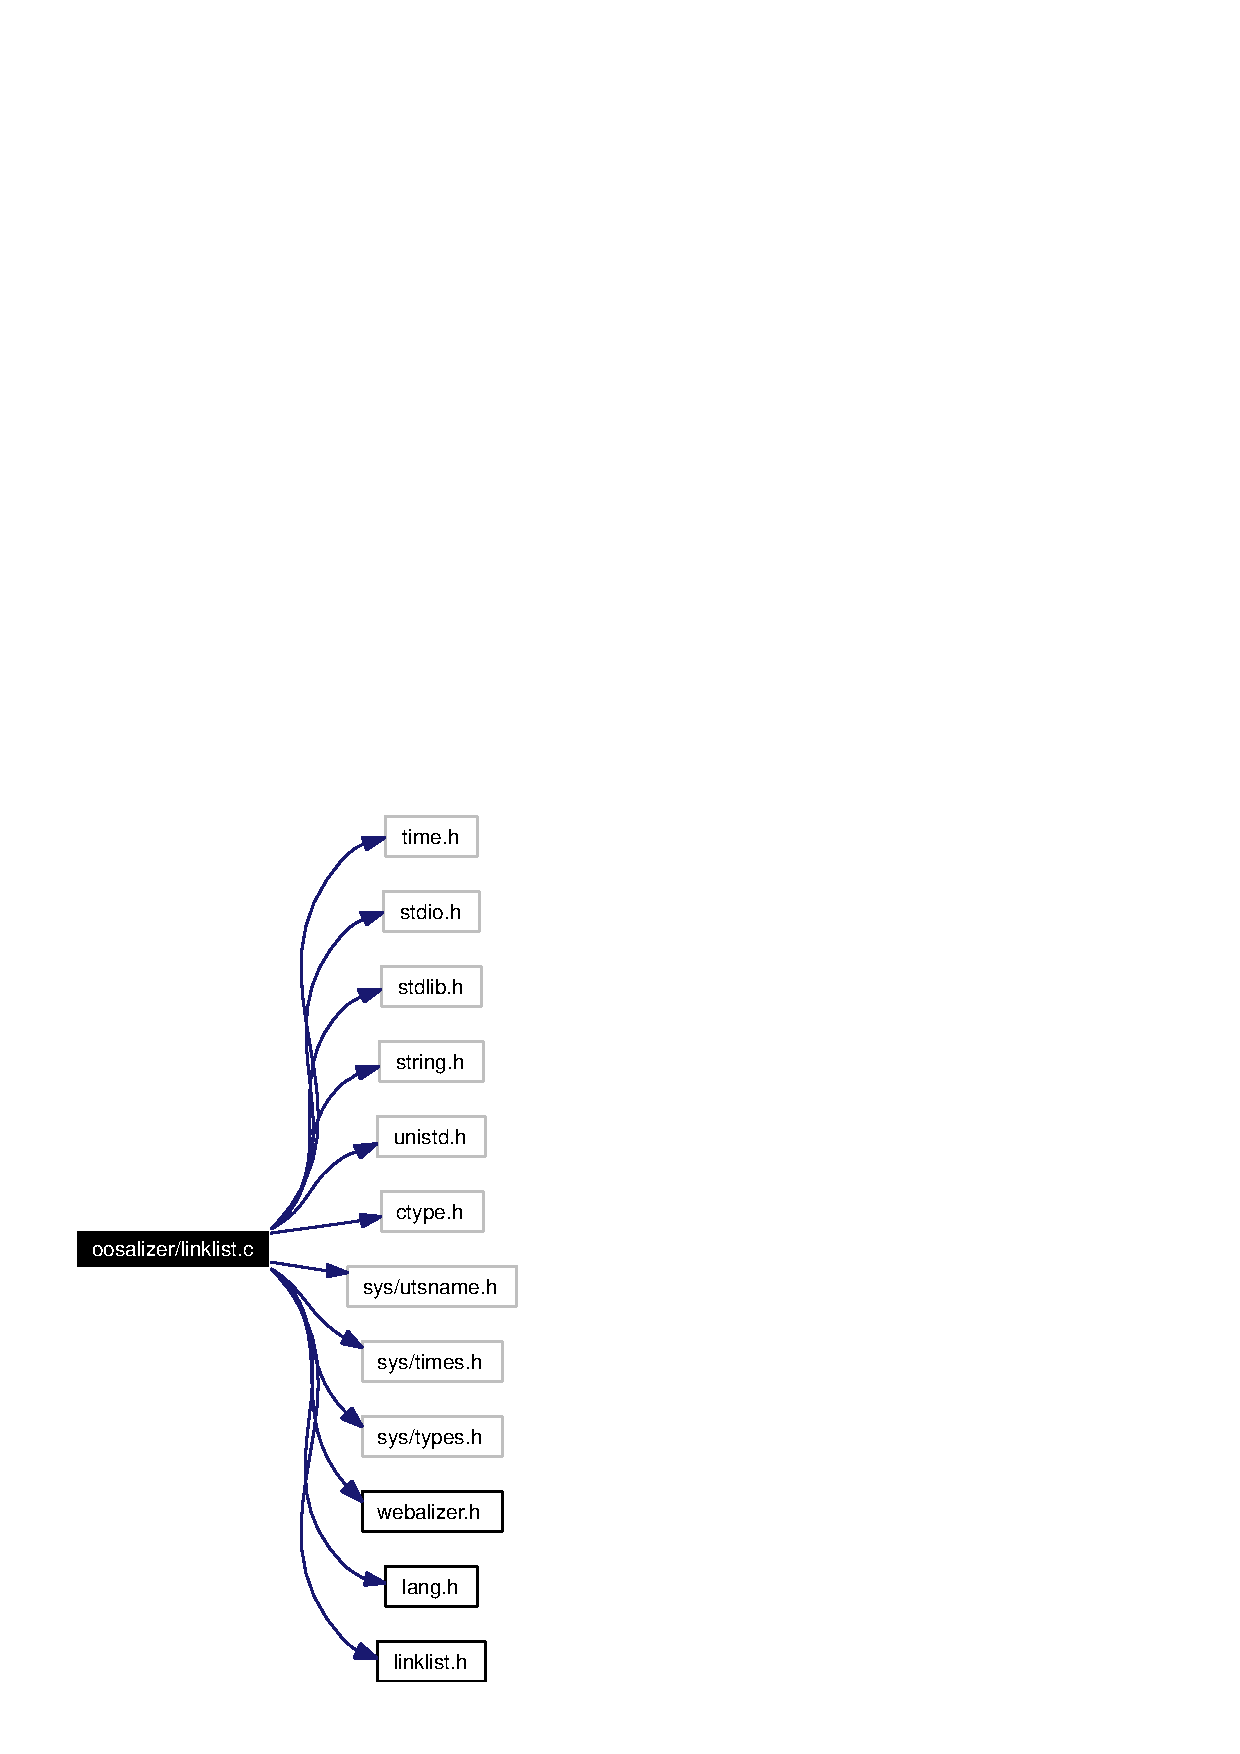
\includegraphics[width=124pt]{linklist_8c__incl}
\end{center}
\end{figure}
\subsection*{Makrodefinitionen}
\begin{CompactItemize}
\item 
\#define {\bf CLK\_\-TCK}~\_\-SC\_\-CLK\_\-TCK
\end{CompactItemize}
\subsection*{Funktionen}
\begin{CompactItemize}
\item 
{\bf NLISTPTR} {\bf new\_\-nlist} (char $\ast$)
\item 
void {\bf del\_\-nlist} ({\bf NLISTPTR} $\ast$)
\item 
{\bf GLISTPTR} {\bf new\_\-glist} (char $\ast$, char $\ast$)
\item 
void {\bf del\_\-glist} ({\bf GLISTPTR} $\ast$)
\item 
int {\bf isinstr} (char $\ast$, char $\ast$)
\item 
int {\bf add\_\-nlist} (char $\ast$str, {\bf NLISTPTR} $\ast$list)
\item 
int {\bf add\_\-glist} (char $\ast$str, {\bf GLISTPTR} $\ast$list)
\item 
char $\ast$ {\bf isinlist} ({\bf NLISTPTR} list, char $\ast$str)
\item 
char $\ast$ {\bf isinglist} ({\bf GLISTPTR} list, char $\ast$str)
\end{CompactItemize}
\subsection*{Variablen}
\begin{CompactItemize}
\item 
{\bf GLISTPTR} {\bf group\_\-sites} = NULL
\item 
{\bf GLISTPTR} {\bf group\_\-urls} = NULL
\item 
{\bf GLISTPTR} {\bf group\_\-refs} = NULL
\item 
{\bf GLISTPTR} {\bf group\_\-agents} = NULL
\item 
{\bf GLISTPTR} {\bf group\_\-users} = NULL
\item 
{\bf NLISTPTR} {\bf hidden\_\-sites} = NULL
\item 
{\bf NLISTPTR} {\bf hidden\_\-urls} = NULL
\item 
{\bf NLISTPTR} {\bf hidden\_\-refs} = NULL
\item 
{\bf NLISTPTR} {\bf hidden\_\-agents} = NULL
\item 
{\bf NLISTPTR} {\bf hidden\_\-users} = NULL
\item 
{\bf NLISTPTR} {\bf ignored\_\-sites} = NULL
\item 
{\bf NLISTPTR} {\bf ignored\_\-urls} = NULL
\item 
{\bf NLISTPTR} {\bf ignored\_\-refs} = NULL
\item 
{\bf NLISTPTR} {\bf ignored\_\-agents} = NULL
\item 
{\bf NLISTPTR} {\bf ignored\_\-users} = NULL
\item 
{\bf NLISTPTR} {\bf include\_\-sites} = NULL
\item 
{\bf NLISTPTR} {\bf include\_\-urls} = NULL
\item 
{\bf NLISTPTR} {\bf include\_\-refs} = NULL
\item 
{\bf NLISTPTR} {\bf include\_\-agents} = NULL
\item 
{\bf NLISTPTR} {\bf include\_\-users} = NULL
\item 
{\bf NLISTPTR} {\bf index\_\-alias} = NULL
\item 
{\bf NLISTPTR} {\bf html\_\-pre} = NULL
\item 
{\bf NLISTPTR} {\bf html\_\-head} = NULL
\item 
{\bf NLISTPTR} {\bf html\_\-body} = NULL
\item 
{\bf NLISTPTR} {\bf html\_\-post} = NULL
\item 
{\bf NLISTPTR} {\bf html\_\-tail} = NULL
\item 
{\bf NLISTPTR} {\bf html\_\-end} = NULL
\item 
{\bf NLISTPTR} {\bf page\_\-type} = NULL
\item 
{\bf GLISTPTR} {\bf search\_\-list} = NULL
\end{CompactItemize}


\subsection{Makro-Dokumentation}
\index{linklist.c@{linklist.c}!CLK_TCK@{CLK\_\-TCK}}
\index{CLK_TCK@{CLK\_\-TCK}!linklist.c@{linklist.c}}
\subsubsection{\setlength{\rightskip}{0pt plus 5cm}\#define CLK\_\-TCK~\_\-SC\_\-CLK\_\-TCK}\label{linklist_8c_03df76d1f70664d745ca8de2864e39b3}




Definiert in Zeile 59 der Datei linklist.c.

\subsection{Dokumentation der Funktionen}
\index{linklist.c@{linklist.c}!add_glist@{add\_\-glist}}
\index{add_glist@{add\_\-glist}!linklist.c@{linklist.c}}
\subsubsection{\setlength{\rightskip}{0pt plus 5cm}int add\_\-glist (char $\ast$ {\em str}, {\bf GLISTPTR} $\ast$ {\em list})}\label{linklist_8c_7a76399c20af4803b0efcc757733039d}




Definiert in Zeile 190 der Datei linklist.c.

Benutzt new\_\-glist() und glist::next.\index{linklist.c@{linklist.c}!add_nlist@{add\_\-nlist}}
\index{add_nlist@{add\_\-nlist}!linklist.c@{linklist.c}}
\subsubsection{\setlength{\rightskip}{0pt plus 5cm}int add\_\-nlist (char $\ast$ {\em str}, {\bf NLISTPTR} $\ast$ {\em list})}\label{linklist_8c_8839d62523e9b12655cca004617bbe77}




Definiert in Zeile 129 der Datei linklist.c.

Benutzt new\_\-nlist() und nlist::next.

Wird benutzt von main().\index{linklist.c@{linklist.c}!del_glist@{del\_\-glist}}
\index{del_glist@{del\_\-glist}!linklist.c@{linklist.c}}
\subsubsection{\setlength{\rightskip}{0pt plus 5cm}void del\_\-glist ({\bf GLISTPTR} $\ast$)}\label{linklist_8c_2db320536d6c5a8726da8e8e627af50c}




Definiert in Zeile 226 der Datei linklist.c.

Benutzt glist::next.\index{linklist.c@{linklist.c}!del_nlist@{del\_\-nlist}}
\index{del_nlist@{del\_\-nlist}!linklist.c@{linklist.c}}
\subsubsection{\setlength{\rightskip}{0pt plus 5cm}void del\_\-nlist ({\bf NLISTPTR} $\ast$)}\label{linklist_8c_949ae6c82d1c88d8407757f05724d8af}




Definiert in Zeile 150 der Datei linklist.c.

Benutzt nlist::next.\index{linklist.c@{linklist.c}!isinglist@{isinglist}}
\index{isinglist@{isinglist}!linklist.c@{linklist.c}}
\subsubsection{\setlength{\rightskip}{0pt plus 5cm}char$\ast$ isinglist ({\bf GLISTPTR} {\em list}, char $\ast$ {\em str})}\label{linklist_8c_70d3ef92faca75f6392ba919975ffe47}




Definiert in Zeile 260 der Datei linklist.c.

Benutzt isinstr(), glist::name, glist::next und glist::string.

Wird benutzt von srch\_\-string().\index{linklist.c@{linklist.c}!isinlist@{isinlist}}
\index{isinlist@{isinlist}!linklist.c@{linklist.c}}
\subsubsection{\setlength{\rightskip}{0pt plus 5cm}char$\ast$ isinlist ({\bf NLISTPTR} {\em list}, char $\ast$ {\em str})}\label{linklist_8c_29bda5ebb6dd2f9b19d8f9519eaf94ff}




Definiert in Zeile 243 der Datei linklist.c.

Benutzt isinstr(), nlist::next und nlist::string.

Wird benutzt von ispage(), main(), put\_\-anode(), put\_\-hnode(), put\_\-inode(), put\_\-rnode() und put\_\-unode().\index{linklist.c@{linklist.c}!isinstr@{isinstr}}
\index{isinstr@{isinstr}!linklist.c@{linklist.c}}
\subsubsection{\setlength{\rightskip}{0pt plus 5cm}int isinstr (char $\ast$, char $\ast$)}\label{linklist_8c_99ef4b81dcab23e1497ea7d5afdeceeb}




Definiert in Zeile 277 der Datei linklist.c.

Wird benutzt von isinglist() und isinlist().\index{linklist.c@{linklist.c}!new_glist@{new\_\-glist}}
\index{new_glist@{new\_\-glist}!linklist.c@{linklist.c}}
\subsubsection{\setlength{\rightskip}{0pt plus 5cm}{\bf GLISTPTR} new\_\-glist (char $\ast$, char $\ast$)}\label{linklist_8c_efe1a363b71eccafc7f2c8e31f8f2b05}




Definiert in Zeile 167 der Datei linklist.c.

Benutzt msg\_\-big\_\-one, glist::name, glist::next, glist::string und verbose.

Wird benutzt von add\_\-glist().\index{linklist.c@{linklist.c}!new_nlist@{new\_\-nlist}}
\index{new_nlist@{new\_\-nlist}!linklist.c@{linklist.c}}
\subsubsection{\setlength{\rightskip}{0pt plus 5cm}{\bf NLISTPTR} new\_\-nlist (char $\ast$)}\label{linklist_8c_2818014b7feb4f6db3a0884d0c7caf0f}




Definiert in Zeile 111 der Datei linklist.c.

Benutzt msg\_\-big\_\-one, nlist::next, nlist::string und verbose.

Wird benutzt von add\_\-nlist().

\subsection{Variablen-Dokumentation}
\index{linklist.c@{linklist.c}!group_agents@{group\_\-agents}}
\index{group_agents@{group\_\-agents}!linklist.c@{linklist.c}}
\subsubsection{\setlength{\rightskip}{0pt plus 5cm}{\bf GLISTPTR} {\bf group\_\-agents} = NULL}\label{linklist_8c_2acbebab9914d67a3cea0f3716324fe2}




Definiert in Zeile 80 der Datei linklist.c.\index{linklist.c@{linklist.c}!group_refs@{group\_\-refs}}
\index{group_refs@{group\_\-refs}!linklist.c@{linklist.c}}
\subsubsection{\setlength{\rightskip}{0pt plus 5cm}{\bf GLISTPTR} {\bf group\_\-refs} = NULL}\label{linklist_8c_73820e36830211218e9c911bc6ea6273}




Definiert in Zeile 79 der Datei linklist.c.\index{linklist.c@{linklist.c}!group_sites@{group\_\-sites}}
\index{group_sites@{group\_\-sites}!linklist.c@{linklist.c}}
\subsubsection{\setlength{\rightskip}{0pt plus 5cm}{\bf GLISTPTR} {\bf group\_\-sites} = NULL}\label{linklist_8c_cda3597076ed2d11c457ee98bb89caa7}




Definiert in Zeile 77 der Datei linklist.c.\index{linklist.c@{linklist.c}!group_urls@{group\_\-urls}}
\index{group_urls@{group\_\-urls}!linklist.c@{linklist.c}}
\subsubsection{\setlength{\rightskip}{0pt plus 5cm}{\bf GLISTPTR} {\bf group\_\-urls} = NULL}\label{linklist_8c_2b91bf4fd34380ee9673b57513dbff01}




Definiert in Zeile 78 der Datei linklist.c.\index{linklist.c@{linklist.c}!group_users@{group\_\-users}}
\index{group_users@{group\_\-users}!linklist.c@{linklist.c}}
\subsubsection{\setlength{\rightskip}{0pt plus 5cm}{\bf GLISTPTR} {\bf group\_\-users} = NULL}\label{linklist_8c_5589f953a1673e7a2f3891d321794340}




Definiert in Zeile 81 der Datei linklist.c.\index{linklist.c@{linklist.c}!hidden_agents@{hidden\_\-agents}}
\index{hidden_agents@{hidden\_\-agents}!linklist.c@{linklist.c}}
\subsubsection{\setlength{\rightskip}{0pt plus 5cm}{\bf NLISTPTR} {\bf hidden\_\-agents} = NULL}\label{linklist_8c_89feb23799329906fbd4a3d47a303027}




Definiert in Zeile 85 der Datei linklist.c.

Wird benutzt von main() und put\_\-anode().\index{linklist.c@{linklist.c}!hidden_refs@{hidden\_\-refs}}
\index{hidden_refs@{hidden\_\-refs}!linklist.c@{linklist.c}}
\subsubsection{\setlength{\rightskip}{0pt plus 5cm}{\bf NLISTPTR} {\bf hidden\_\-refs} = NULL}\label{linklist_8c_7f8ec975eaff8227a3e09efb17d3e064}




Definiert in Zeile 84 der Datei linklist.c.

Wird benutzt von main() und put\_\-rnode().\index{linklist.c@{linklist.c}!hidden_sites@{hidden\_\-sites}}
\index{hidden_sites@{hidden\_\-sites}!linklist.c@{linklist.c}}
\subsubsection{\setlength{\rightskip}{0pt plus 5cm}{\bf NLISTPTR} {\bf hidden\_\-sites} = NULL}\label{linklist_8c_96bde86b735761b0b2b03d057d7bddfd}




Definiert in Zeile 82 der Datei linklist.c.

Wird benutzt von main() und put\_\-hnode().\index{linklist.c@{linklist.c}!hidden_urls@{hidden\_\-urls}}
\index{hidden_urls@{hidden\_\-urls}!linklist.c@{linklist.c}}
\subsubsection{\setlength{\rightskip}{0pt plus 5cm}{\bf NLISTPTR} {\bf hidden\_\-urls} = NULL}\label{linklist_8c_fb86638f144a8726901b06185e2415af}




Definiert in Zeile 83 der Datei linklist.c.

Wird benutzt von main() und put\_\-unode().\index{linklist.c@{linklist.c}!hidden_users@{hidden\_\-users}}
\index{hidden_users@{hidden\_\-users}!linklist.c@{linklist.c}}
\subsubsection{\setlength{\rightskip}{0pt plus 5cm}{\bf NLISTPTR} {\bf hidden\_\-users} = NULL}\label{linklist_8c_c328ffff94e0ce5d57817ee1197767aa}




Definiert in Zeile 86 der Datei linklist.c.

Wird benutzt von put\_\-inode().\index{linklist.c@{linklist.c}!html_body@{html\_\-body}}
\index{html_body@{html\_\-body}!linklist.c@{linklist.c}}
\subsubsection{\setlength{\rightskip}{0pt plus 5cm}{\bf NLISTPTR} {\bf html\_\-body} = NULL}\label{linklist_8c_4bb0bd1db8f0b3cc89d509d8c5daddde}




Definiert in Zeile 100 der Datei linklist.c.

Wird benutzt von write\_\-html\_\-head().\index{linklist.c@{linklist.c}!html_end@{html\_\-end}}
\index{html_end@{html\_\-end}!linklist.c@{linklist.c}}
\subsubsection{\setlength{\rightskip}{0pt plus 5cm}{\bf NLISTPTR} {\bf html\_\-end} = NULL}\label{linklist_8c_d7f0906501b524d986d95f8efddb48e5}




Definiert in Zeile 103 der Datei linklist.c.

Wird benutzt von write\_\-html\_\-tail().\index{linklist.c@{linklist.c}!html_head@{html\_\-head}}
\index{html_head@{html\_\-head}!linklist.c@{linklist.c}}
\subsubsection{\setlength{\rightskip}{0pt plus 5cm}{\bf NLISTPTR} {\bf html\_\-head} = NULL}\label{linklist_8c_1811e9595e278ef4ac307d06cd3a4eed}




Definiert in Zeile 99 der Datei linklist.c.

Wird benutzt von write\_\-html\_\-head().\index{linklist.c@{linklist.c}!html_post@{html\_\-post}}
\index{html_post@{html\_\-post}!linklist.c@{linklist.c}}
\subsubsection{\setlength{\rightskip}{0pt plus 5cm}{\bf NLISTPTR} {\bf html\_\-post} = NULL}\label{linklist_8c_fd6de839e46d75632279853537235e7c}




Definiert in Zeile 101 der Datei linklist.c.

Wird benutzt von write\_\-html\_\-head().\index{linklist.c@{linklist.c}!html_pre@{html\_\-pre}}
\index{html_pre@{html\_\-pre}!linklist.c@{linklist.c}}
\subsubsection{\setlength{\rightskip}{0pt plus 5cm}{\bf NLISTPTR} {\bf html\_\-pre} = NULL}\label{linklist_8c_cea32428cfbcce0e252dd3613586d0f3}




Definiert in Zeile 98 der Datei linklist.c.

Wird benutzt von write\_\-html\_\-head().\index{linklist.c@{linklist.c}!html_tail@{html\_\-tail}}
\index{html_tail@{html\_\-tail}!linklist.c@{linklist.c}}
\subsubsection{\setlength{\rightskip}{0pt plus 5cm}{\bf NLISTPTR} {\bf html\_\-tail} = NULL}\label{linklist_8c_7d3b981f0cda9084a93c191ab80637da}




Definiert in Zeile 102 der Datei linklist.c.

Wird benutzt von write\_\-html\_\-tail().\index{linklist.c@{linklist.c}!ignored_agents@{ignored\_\-agents}}
\index{ignored_agents@{ignored\_\-agents}!linklist.c@{linklist.c}}
\subsubsection{\setlength{\rightskip}{0pt plus 5cm}{\bf NLISTPTR} {\bf ignored\_\-agents} = NULL}\label{linklist_8c_60013ce10d008e9eb74a4b6f28959729}




Definiert in Zeile 90 der Datei linklist.c.\index{linklist.c@{linklist.c}!ignored_refs@{ignored\_\-refs}}
\index{ignored_refs@{ignored\_\-refs}!linklist.c@{linklist.c}}
\subsubsection{\setlength{\rightskip}{0pt plus 5cm}{\bf NLISTPTR} {\bf ignored\_\-refs} = NULL}\label{linklist_8c_761639dc29cca53d524007b9fb4a6e65}




Definiert in Zeile 89 der Datei linklist.c.\index{linklist.c@{linklist.c}!ignored_sites@{ignored\_\-sites}}
\index{ignored_sites@{ignored\_\-sites}!linklist.c@{linklist.c}}
\subsubsection{\setlength{\rightskip}{0pt plus 5cm}{\bf NLISTPTR} {\bf ignored\_\-sites} = NULL}\label{linklist_8c_9df089ae5b8931353b2e79b9a33c70e6}




Definiert in Zeile 87 der Datei linklist.c.\index{linklist.c@{linklist.c}!ignored_urls@{ignored\_\-urls}}
\index{ignored_urls@{ignored\_\-urls}!linklist.c@{linklist.c}}
\subsubsection{\setlength{\rightskip}{0pt plus 5cm}{\bf NLISTPTR} {\bf ignored\_\-urls} = NULL}\label{linklist_8c_9a30b4cfe3e814caad5864bf70683264}




Definiert in Zeile 88 der Datei linklist.c.\index{linklist.c@{linklist.c}!ignored_users@{ignored\_\-users}}
\index{ignored_users@{ignored\_\-users}!linklist.c@{linklist.c}}
\subsubsection{\setlength{\rightskip}{0pt plus 5cm}{\bf NLISTPTR} {\bf ignored\_\-users} = NULL}\label{linklist_8c_c61949a50def3ceeaf32f93f01d1ea16}




Definiert in Zeile 91 der Datei linklist.c.\index{linklist.c@{linklist.c}!include_agents@{include\_\-agents}}
\index{include_agents@{include\_\-agents}!linklist.c@{linklist.c}}
\subsubsection{\setlength{\rightskip}{0pt plus 5cm}{\bf NLISTPTR} {\bf include\_\-agents} = NULL}\label{linklist_8c_29034f7c35846ae0399bd7b358be1d94}




Definiert in Zeile 95 der Datei linklist.c.\index{linklist.c@{linklist.c}!include_refs@{include\_\-refs}}
\index{include_refs@{include\_\-refs}!linklist.c@{linklist.c}}
\subsubsection{\setlength{\rightskip}{0pt plus 5cm}{\bf NLISTPTR} {\bf include\_\-refs} = NULL}\label{linklist_8c_72e046ed2702acb3b3cc2aa444f861b0}




Definiert in Zeile 94 der Datei linklist.c.\index{linklist.c@{linklist.c}!include_sites@{include\_\-sites}}
\index{include_sites@{include\_\-sites}!linklist.c@{linklist.c}}
\subsubsection{\setlength{\rightskip}{0pt plus 5cm}{\bf NLISTPTR} {\bf include\_\-sites} = NULL}\label{linklist_8c_54c446a5497d9c6f94704e50f3ab099f}




Definiert in Zeile 92 der Datei linklist.c.\index{linklist.c@{linklist.c}!include_urls@{include\_\-urls}}
\index{include_urls@{include\_\-urls}!linklist.c@{linklist.c}}
\subsubsection{\setlength{\rightskip}{0pt plus 5cm}{\bf NLISTPTR} {\bf include\_\-urls} = NULL}\label{linklist_8c_10e92b92241988092187d4a28d95d057}




Definiert in Zeile 93 der Datei linklist.c.\index{linklist.c@{linklist.c}!include_users@{include\_\-users}}
\index{include_users@{include\_\-users}!linklist.c@{linklist.c}}
\subsubsection{\setlength{\rightskip}{0pt plus 5cm}{\bf NLISTPTR} {\bf include\_\-users} = NULL}\label{linklist_8c_4301d92f7f72fdda0af03033d967155b}




Definiert in Zeile 96 der Datei linklist.c.\index{linklist.c@{linklist.c}!index_alias@{index\_\-alias}}
\index{index_alias@{index\_\-alias}!linklist.c@{linklist.c}}
\subsubsection{\setlength{\rightskip}{0pt plus 5cm}{\bf NLISTPTR} {\bf index\_\-alias} = NULL}\label{linklist_8c_a35b4fc28f26c83f77336185f9aa7175}




Definiert in Zeile 97 der Datei linklist.c.

Wird benutzt von main().\index{linklist.c@{linklist.c}!page_type@{page\_\-type}}
\index{page_type@{page\_\-type}!linklist.c@{linklist.c}}
\subsubsection{\setlength{\rightskip}{0pt plus 5cm}{\bf NLISTPTR} {\bf page\_\-type} = NULL}\label{linklist_8c_556b3c90c27ba5b38626945734914353}




Definiert in Zeile 104 der Datei linklist.c.

Wird benutzt von ispage() und main().\index{linklist.c@{linklist.c}!search_list@{search\_\-list}}
\index{search_list@{search\_\-list}!linklist.c@{linklist.c}}
\subsubsection{\setlength{\rightskip}{0pt plus 5cm}{\bf GLISTPTR} {\bf search\_\-list} = NULL}\label{linklist_8c_d93c06cbf86de996601e602d07da3663}




Definiert in Zeile 105 der Datei linklist.c.

Wird benutzt von srch\_\-string().
\section{oosalizer/linklist.h-Dateireferenz}
\label{linklist_8h}\index{oosalizer/linklist.h@{oosalizer/linklist.h}}


Dieser Graph zeigt, welche Datei direkt oder indirekt diese Datei enth\"{a}lt:\begin{figure}[H]
\begin{center}
\leavevmode
\includegraphics[width=139pt]{linklist_8h__dep__incl}
\end{center}
\end{figure}
\subsection*{Datenstrukturen}
\begin{CompactItemize}
\item 
struct {\bf nlist}
\item 
struct {\bf glist}
\end{CompactItemize}
\subsection*{Typdefinitionen}
\begin{CompactItemize}
\item 
typedef {\bf nlist} $\ast$ {\bf NLISTPTR}
\item 
typedef {\bf glist} $\ast$ {\bf GLISTPTR}
\end{CompactItemize}
\subsection*{Funktionen}
\begin{CompactItemize}
\item 
char $\ast$ {\bf isinlist} ({\bf NLISTPTR}, char $\ast$)
\item 
char $\ast$ {\bf isinglist} ({\bf GLISTPTR}, char $\ast$)
\item 
int {\bf add\_\-nlist} (char $\ast$, {\bf NLISTPTR} $\ast$)
\item 
int {\bf add\_\-glist} (char $\ast$, {\bf GLISTPTR} $\ast$)
\end{CompactItemize}
\subsection*{Variablen}
\begin{CompactItemize}
\item 
{\bf GLISTPTR} {\bf group\_\-sites}
\item 
{\bf GLISTPTR} {\bf group\_\-urls}
\item 
{\bf GLISTPTR} {\bf group\_\-refs}
\item 
{\bf GLISTPTR} {\bf group\_\-agents}
\item 
{\bf GLISTPTR} {\bf group\_\-users}
\item 
{\bf NLISTPTR} {\bf hidden\_\-sites}
\item 
{\bf NLISTPTR} {\bf hidden\_\-urls}
\item 
{\bf NLISTPTR} {\bf hidden\_\-refs}
\item 
{\bf NLISTPTR} {\bf hidden\_\-agents}
\item 
{\bf NLISTPTR} {\bf hidden\_\-users}
\item 
{\bf NLISTPTR} {\bf ignored\_\-sites}
\item 
{\bf NLISTPTR} {\bf ignored\_\-urls}
\item 
{\bf NLISTPTR} {\bf ignored\_\-refs}
\item 
{\bf NLISTPTR} {\bf ignored\_\-agents}
\item 
{\bf NLISTPTR} {\bf ignored\_\-users}
\item 
{\bf NLISTPTR} {\bf include\_\-sites}
\item 
{\bf NLISTPTR} {\bf include\_\-urls}
\item 
{\bf NLISTPTR} {\bf include\_\-refs}
\item 
{\bf NLISTPTR} {\bf include\_\-agents}
\item 
{\bf NLISTPTR} {\bf include\_\-users}
\item 
{\bf NLISTPTR} {\bf index\_\-alias}
\item 
{\bf NLISTPTR} {\bf html\_\-pre}
\item 
{\bf NLISTPTR} {\bf html\_\-head}
\item 
{\bf NLISTPTR} {\bf html\_\-body}
\item 
{\bf NLISTPTR} {\bf html\_\-post}
\item 
{\bf NLISTPTR} {\bf html\_\-tail}
\item 
{\bf NLISTPTR} {\bf html\_\-end}
\item 
{\bf NLISTPTR} {\bf page\_\-type}
\item 
{\bf GLISTPTR} {\bf search\_\-list}
\end{CompactItemize}


\subsection{Dokumentation der benutzerdefinierten Typen}
\index{linklist.h@{linklist.h}!GLISTPTR@{GLISTPTR}}
\index{GLISTPTR@{GLISTPTR}!linklist.h@{linklist.h}}
\subsubsection{\setlength{\rightskip}{0pt plus 5cm}typedef struct {\bf glist}$\ast$ {\bf GLISTPTR}}\label{linklist_8h_8ba38064a5a49a77b788338c8aab0ce9}




Definiert in Zeile 11 der Datei linklist.h.\index{linklist.h@{linklist.h}!NLISTPTR@{NLISTPTR}}
\index{NLISTPTR@{NLISTPTR}!linklist.h@{linklist.h}}
\subsubsection{\setlength{\rightskip}{0pt plus 5cm}typedef struct {\bf nlist}$\ast$ {\bf NLISTPTR}}\label{linklist_8h_a24a845f5406aa82c81d3d1b74fa7c87}




Definiert in Zeile 6 der Datei linklist.h.

\subsection{Dokumentation der Funktionen}
\index{linklist.h@{linklist.h}!add_glist@{add\_\-glist}}
\index{add_glist@{add\_\-glist}!linklist.h@{linklist.h}}
\subsubsection{\setlength{\rightskip}{0pt plus 5cm}int add\_\-glist (char $\ast$, {\bf GLISTPTR} $\ast$)}\label{linklist_8h_a17a4a0e1bebcb1f19644843920ef3ea}




Definiert in Zeile 190 der Datei linklist.c.

Benutzt new\_\-glist() und glist::next.\index{linklist.h@{linklist.h}!add_nlist@{add\_\-nlist}}
\index{add_nlist@{add\_\-nlist}!linklist.h@{linklist.h}}
\subsubsection{\setlength{\rightskip}{0pt plus 5cm}int add\_\-nlist (char $\ast$, {\bf NLISTPTR} $\ast$)}\label{linklist_8h_5ff4c7ffc3201d64048a6921c866c937}




Definiert in Zeile 129 der Datei linklist.c.

Benutzt new\_\-nlist() und nlist::next.

Wird benutzt von main().\index{linklist.h@{linklist.h}!isinglist@{isinglist}}
\index{isinglist@{isinglist}!linklist.h@{linklist.h}}
\subsubsection{\setlength{\rightskip}{0pt plus 5cm}char$\ast$ isinglist ({\bf GLISTPTR}, char $\ast$)}\label{linklist_8h_04dff50c01cd9572b6a3d9dfbdb7cc07}




Definiert in Zeile 260 der Datei linklist.c.

Benutzt isinstr(), glist::name, glist::next und glist::string.

Wird benutzt von srch\_\-string().\index{linklist.h@{linklist.h}!isinlist@{isinlist}}
\index{isinlist@{isinlist}!linklist.h@{linklist.h}}
\subsubsection{\setlength{\rightskip}{0pt plus 5cm}char$\ast$ isinlist ({\bf NLISTPTR}, char $\ast$)}\label{linklist_8h_3568dfb8e887fc7a6c38ca8f900c721c}




Definiert in Zeile 243 der Datei linklist.c.

Benutzt isinstr(), nlist::next und nlist::string.

Wird benutzt von ispage(), main(), put\_\-anode(), put\_\-hnode(), put\_\-inode(), put\_\-rnode() und put\_\-unode().

\subsection{Variablen-Dokumentation}
\index{linklist.h@{linklist.h}!group_agents@{group\_\-agents}}
\index{group_agents@{group\_\-agents}!linklist.h@{linklist.h}}
\subsubsection{\setlength{\rightskip}{0pt plus 5cm}{\bf GLISTPTR} {\bf group\_\-agents}}\label{linklist_8h_2acbebab9914d67a3cea0f3716324fe2}




Definiert in Zeile 80 der Datei linklist.c.\index{linklist.h@{linklist.h}!group_refs@{group\_\-refs}}
\index{group_refs@{group\_\-refs}!linklist.h@{linklist.h}}
\subsubsection{\setlength{\rightskip}{0pt plus 5cm}{\bf GLISTPTR} {\bf group\_\-refs}}\label{linklist_8h_73820e36830211218e9c911bc6ea6273}




Definiert in Zeile 79 der Datei linklist.c.\index{linklist.h@{linklist.h}!group_sites@{group\_\-sites}}
\index{group_sites@{group\_\-sites}!linklist.h@{linklist.h}}
\subsubsection{\setlength{\rightskip}{0pt plus 5cm}{\bf GLISTPTR} {\bf group\_\-sites}}\label{linklist_8h_cda3597076ed2d11c457ee98bb89caa7}




Definiert in Zeile 77 der Datei linklist.c.\index{linklist.h@{linklist.h}!group_urls@{group\_\-urls}}
\index{group_urls@{group\_\-urls}!linklist.h@{linklist.h}}
\subsubsection{\setlength{\rightskip}{0pt plus 5cm}{\bf GLISTPTR} {\bf group\_\-urls}}\label{linklist_8h_2b91bf4fd34380ee9673b57513dbff01}




Definiert in Zeile 78 der Datei linklist.c.\index{linklist.h@{linklist.h}!group_users@{group\_\-users}}
\index{group_users@{group\_\-users}!linklist.h@{linklist.h}}
\subsubsection{\setlength{\rightskip}{0pt plus 5cm}{\bf GLISTPTR} {\bf group\_\-users}}\label{linklist_8h_5589f953a1673e7a2f3891d321794340}




Definiert in Zeile 81 der Datei linklist.c.\index{linklist.h@{linklist.h}!hidden_agents@{hidden\_\-agents}}
\index{hidden_agents@{hidden\_\-agents}!linklist.h@{linklist.h}}
\subsubsection{\setlength{\rightskip}{0pt plus 5cm}{\bf NLISTPTR} {\bf hidden\_\-agents}}\label{linklist_8h_89feb23799329906fbd4a3d47a303027}




Definiert in Zeile 85 der Datei linklist.c.

Wird benutzt von main() und put\_\-anode().\index{linklist.h@{linklist.h}!hidden_refs@{hidden\_\-refs}}
\index{hidden_refs@{hidden\_\-refs}!linklist.h@{linklist.h}}
\subsubsection{\setlength{\rightskip}{0pt plus 5cm}{\bf NLISTPTR} {\bf hidden\_\-refs}}\label{linklist_8h_7f8ec975eaff8227a3e09efb17d3e064}




Definiert in Zeile 84 der Datei linklist.c.

Wird benutzt von main() und put\_\-rnode().\index{linklist.h@{linklist.h}!hidden_sites@{hidden\_\-sites}}
\index{hidden_sites@{hidden\_\-sites}!linklist.h@{linklist.h}}
\subsubsection{\setlength{\rightskip}{0pt plus 5cm}{\bf NLISTPTR} {\bf hidden\_\-sites}}\label{linklist_8h_96bde86b735761b0b2b03d057d7bddfd}




Definiert in Zeile 82 der Datei linklist.c.

Wird benutzt von main() und put\_\-hnode().\index{linklist.h@{linklist.h}!hidden_urls@{hidden\_\-urls}}
\index{hidden_urls@{hidden\_\-urls}!linklist.h@{linklist.h}}
\subsubsection{\setlength{\rightskip}{0pt plus 5cm}{\bf NLISTPTR} {\bf hidden\_\-urls}}\label{linklist_8h_fb86638f144a8726901b06185e2415af}




Definiert in Zeile 83 der Datei linklist.c.

Wird benutzt von main() und put\_\-unode().\index{linklist.h@{linklist.h}!hidden_users@{hidden\_\-users}}
\index{hidden_users@{hidden\_\-users}!linklist.h@{linklist.h}}
\subsubsection{\setlength{\rightskip}{0pt plus 5cm}{\bf NLISTPTR} {\bf hidden\_\-users}}\label{linklist_8h_c328ffff94e0ce5d57817ee1197767aa}




Definiert in Zeile 86 der Datei linklist.c.

Wird benutzt von put\_\-inode().\index{linklist.h@{linklist.h}!html_body@{html\_\-body}}
\index{html_body@{html\_\-body}!linklist.h@{linklist.h}}
\subsubsection{\setlength{\rightskip}{0pt plus 5cm}{\bf NLISTPTR} {\bf html\_\-body}}\label{linklist_8h_4bb0bd1db8f0b3cc89d509d8c5daddde}




Definiert in Zeile 100 der Datei linklist.c.

Wird benutzt von write\_\-html\_\-head().\index{linklist.h@{linklist.h}!html_end@{html\_\-end}}
\index{html_end@{html\_\-end}!linklist.h@{linklist.h}}
\subsubsection{\setlength{\rightskip}{0pt plus 5cm}{\bf NLISTPTR} {\bf html\_\-end}}\label{linklist_8h_d7f0906501b524d986d95f8efddb48e5}




Definiert in Zeile 103 der Datei linklist.c.

Wird benutzt von write\_\-html\_\-tail().\index{linklist.h@{linklist.h}!html_head@{html\_\-head}}
\index{html_head@{html\_\-head}!linklist.h@{linklist.h}}
\subsubsection{\setlength{\rightskip}{0pt plus 5cm}{\bf NLISTPTR} {\bf html\_\-head}}\label{linklist_8h_1811e9595e278ef4ac307d06cd3a4eed}




Definiert in Zeile 99 der Datei linklist.c.

Wird benutzt von write\_\-html\_\-head().\index{linklist.h@{linklist.h}!html_post@{html\_\-post}}
\index{html_post@{html\_\-post}!linklist.h@{linklist.h}}
\subsubsection{\setlength{\rightskip}{0pt plus 5cm}{\bf NLISTPTR} {\bf html\_\-post}}\label{linklist_8h_fd6de839e46d75632279853537235e7c}




Definiert in Zeile 101 der Datei linklist.c.

Wird benutzt von write\_\-html\_\-head().\index{linklist.h@{linklist.h}!html_pre@{html\_\-pre}}
\index{html_pre@{html\_\-pre}!linklist.h@{linklist.h}}
\subsubsection{\setlength{\rightskip}{0pt plus 5cm}{\bf NLISTPTR} {\bf html\_\-pre}}\label{linklist_8h_cea32428cfbcce0e252dd3613586d0f3}




Definiert in Zeile 98 der Datei linklist.c.

Wird benutzt von write\_\-html\_\-head().\index{linklist.h@{linklist.h}!html_tail@{html\_\-tail}}
\index{html_tail@{html\_\-tail}!linklist.h@{linklist.h}}
\subsubsection{\setlength{\rightskip}{0pt plus 5cm}{\bf NLISTPTR} {\bf html\_\-tail}}\label{linklist_8h_7d3b981f0cda9084a93c191ab80637da}




Definiert in Zeile 102 der Datei linklist.c.

Wird benutzt von write\_\-html\_\-tail().\index{linklist.h@{linklist.h}!ignored_agents@{ignored\_\-agents}}
\index{ignored_agents@{ignored\_\-agents}!linklist.h@{linklist.h}}
\subsubsection{\setlength{\rightskip}{0pt plus 5cm}{\bf NLISTPTR} {\bf ignored\_\-agents}}\label{linklist_8h_60013ce10d008e9eb74a4b6f28959729}




Definiert in Zeile 90 der Datei linklist.c.\index{linklist.h@{linklist.h}!ignored_refs@{ignored\_\-refs}}
\index{ignored_refs@{ignored\_\-refs}!linklist.h@{linklist.h}}
\subsubsection{\setlength{\rightskip}{0pt plus 5cm}{\bf NLISTPTR} {\bf ignored\_\-refs}}\label{linklist_8h_761639dc29cca53d524007b9fb4a6e65}




Definiert in Zeile 89 der Datei linklist.c.\index{linklist.h@{linklist.h}!ignored_sites@{ignored\_\-sites}}
\index{ignored_sites@{ignored\_\-sites}!linklist.h@{linklist.h}}
\subsubsection{\setlength{\rightskip}{0pt plus 5cm}{\bf NLISTPTR} {\bf ignored\_\-sites}}\label{linklist_8h_9df089ae5b8931353b2e79b9a33c70e6}




Definiert in Zeile 87 der Datei linklist.c.\index{linklist.h@{linklist.h}!ignored_urls@{ignored\_\-urls}}
\index{ignored_urls@{ignored\_\-urls}!linklist.h@{linklist.h}}
\subsubsection{\setlength{\rightskip}{0pt plus 5cm}{\bf NLISTPTR} {\bf ignored\_\-urls}}\label{linklist_8h_9a30b4cfe3e814caad5864bf70683264}




Definiert in Zeile 88 der Datei linklist.c.\index{linklist.h@{linklist.h}!ignored_users@{ignored\_\-users}}
\index{ignored_users@{ignored\_\-users}!linklist.h@{linklist.h}}
\subsubsection{\setlength{\rightskip}{0pt plus 5cm}{\bf NLISTPTR} {\bf ignored\_\-users}}\label{linklist_8h_c61949a50def3ceeaf32f93f01d1ea16}




Definiert in Zeile 91 der Datei linklist.c.\index{linklist.h@{linklist.h}!include_agents@{include\_\-agents}}
\index{include_agents@{include\_\-agents}!linklist.h@{linklist.h}}
\subsubsection{\setlength{\rightskip}{0pt plus 5cm}{\bf NLISTPTR} {\bf include\_\-agents}}\label{linklist_8h_29034f7c35846ae0399bd7b358be1d94}




Definiert in Zeile 95 der Datei linklist.c.\index{linklist.h@{linklist.h}!include_refs@{include\_\-refs}}
\index{include_refs@{include\_\-refs}!linklist.h@{linklist.h}}
\subsubsection{\setlength{\rightskip}{0pt plus 5cm}{\bf NLISTPTR} {\bf include\_\-refs}}\label{linklist_8h_72e046ed2702acb3b3cc2aa444f861b0}




Definiert in Zeile 94 der Datei linklist.c.\index{linklist.h@{linklist.h}!include_sites@{include\_\-sites}}
\index{include_sites@{include\_\-sites}!linklist.h@{linklist.h}}
\subsubsection{\setlength{\rightskip}{0pt plus 5cm}{\bf NLISTPTR} {\bf include\_\-sites}}\label{linklist_8h_54c446a5497d9c6f94704e50f3ab099f}




Definiert in Zeile 92 der Datei linklist.c.\index{linklist.h@{linklist.h}!include_urls@{include\_\-urls}}
\index{include_urls@{include\_\-urls}!linklist.h@{linklist.h}}
\subsubsection{\setlength{\rightskip}{0pt plus 5cm}{\bf NLISTPTR} {\bf include\_\-urls}}\label{linklist_8h_10e92b92241988092187d4a28d95d057}




Definiert in Zeile 93 der Datei linklist.c.\index{linklist.h@{linklist.h}!include_users@{include\_\-users}}
\index{include_users@{include\_\-users}!linklist.h@{linklist.h}}
\subsubsection{\setlength{\rightskip}{0pt plus 5cm}{\bf NLISTPTR} {\bf include\_\-users}}\label{linklist_8h_4301d92f7f72fdda0af03033d967155b}




Definiert in Zeile 96 der Datei linklist.c.\index{linklist.h@{linklist.h}!index_alias@{index\_\-alias}}
\index{index_alias@{index\_\-alias}!linklist.h@{linklist.h}}
\subsubsection{\setlength{\rightskip}{0pt plus 5cm}{\bf NLISTPTR} {\bf index\_\-alias}}\label{linklist_8h_a35b4fc28f26c83f77336185f9aa7175}




Definiert in Zeile 97 der Datei linklist.c.

Wird benutzt von main().\index{linklist.h@{linklist.h}!page_type@{page\_\-type}}
\index{page_type@{page\_\-type}!linklist.h@{linklist.h}}
\subsubsection{\setlength{\rightskip}{0pt plus 5cm}{\bf NLISTPTR} {\bf page\_\-type}}\label{linklist_8h_556b3c90c27ba5b38626945734914353}




Definiert in Zeile 104 der Datei linklist.c.

Wird benutzt von ispage() und main().\index{linklist.h@{linklist.h}!search_list@{search\_\-list}}
\index{search_list@{search\_\-list}!linklist.h@{linklist.h}}
\subsubsection{\setlength{\rightskip}{0pt plus 5cm}{\bf GLISTPTR} {\bf search\_\-list}}\label{linklist_8h_d93c06cbf86de996601e602d07da3663}




Definiert in Zeile 105 der Datei linklist.c.

Wird benutzt von srch\_\-string().
\section{oosalizer/output.c-Dateireferenz}
\label{output_8c}\index{oosalizer/output.c@{oosalizer/output.c}}
{\tt \#include $<$time.h$>$}\par
{\tt \#include $<$stdio.h$>$}\par
{\tt \#include $<$stdlib.h$>$}\par
{\tt \#include $<$string.h$>$}\par
{\tt \#include $<$unistd.h$>$}\par
{\tt \#include $<$ctype.h$>$}\par
{\tt \#include $<$sys/utsname.h$>$}\par
{\tt \#include $<$sys/times.h$>$}\par
{\tt \#include $<$sys/types.h$>$}\par
{\tt \#include \char`\"{}webalizer.h\char`\"{}}\par
{\tt \#include \char`\"{}lang.h\char`\"{}}\par
{\tt \#include \char`\"{}hashtab.h\char`\"{}}\par
{\tt \#include \char`\"{}preserve.h\char`\"{}}\par
{\tt \#include \char`\"{}linklist.h\char`\"{}}\par
{\tt \#include \char`\"{}graphs.h\char`\"{}}\par
{\tt \#include \char`\"{}output.h\char`\"{}}\par


Include-Abh\"{a}ngigkeitsdiagramm f\"{u}r output.c:\begin{figure}[H]
\begin{center}
\leavevmode
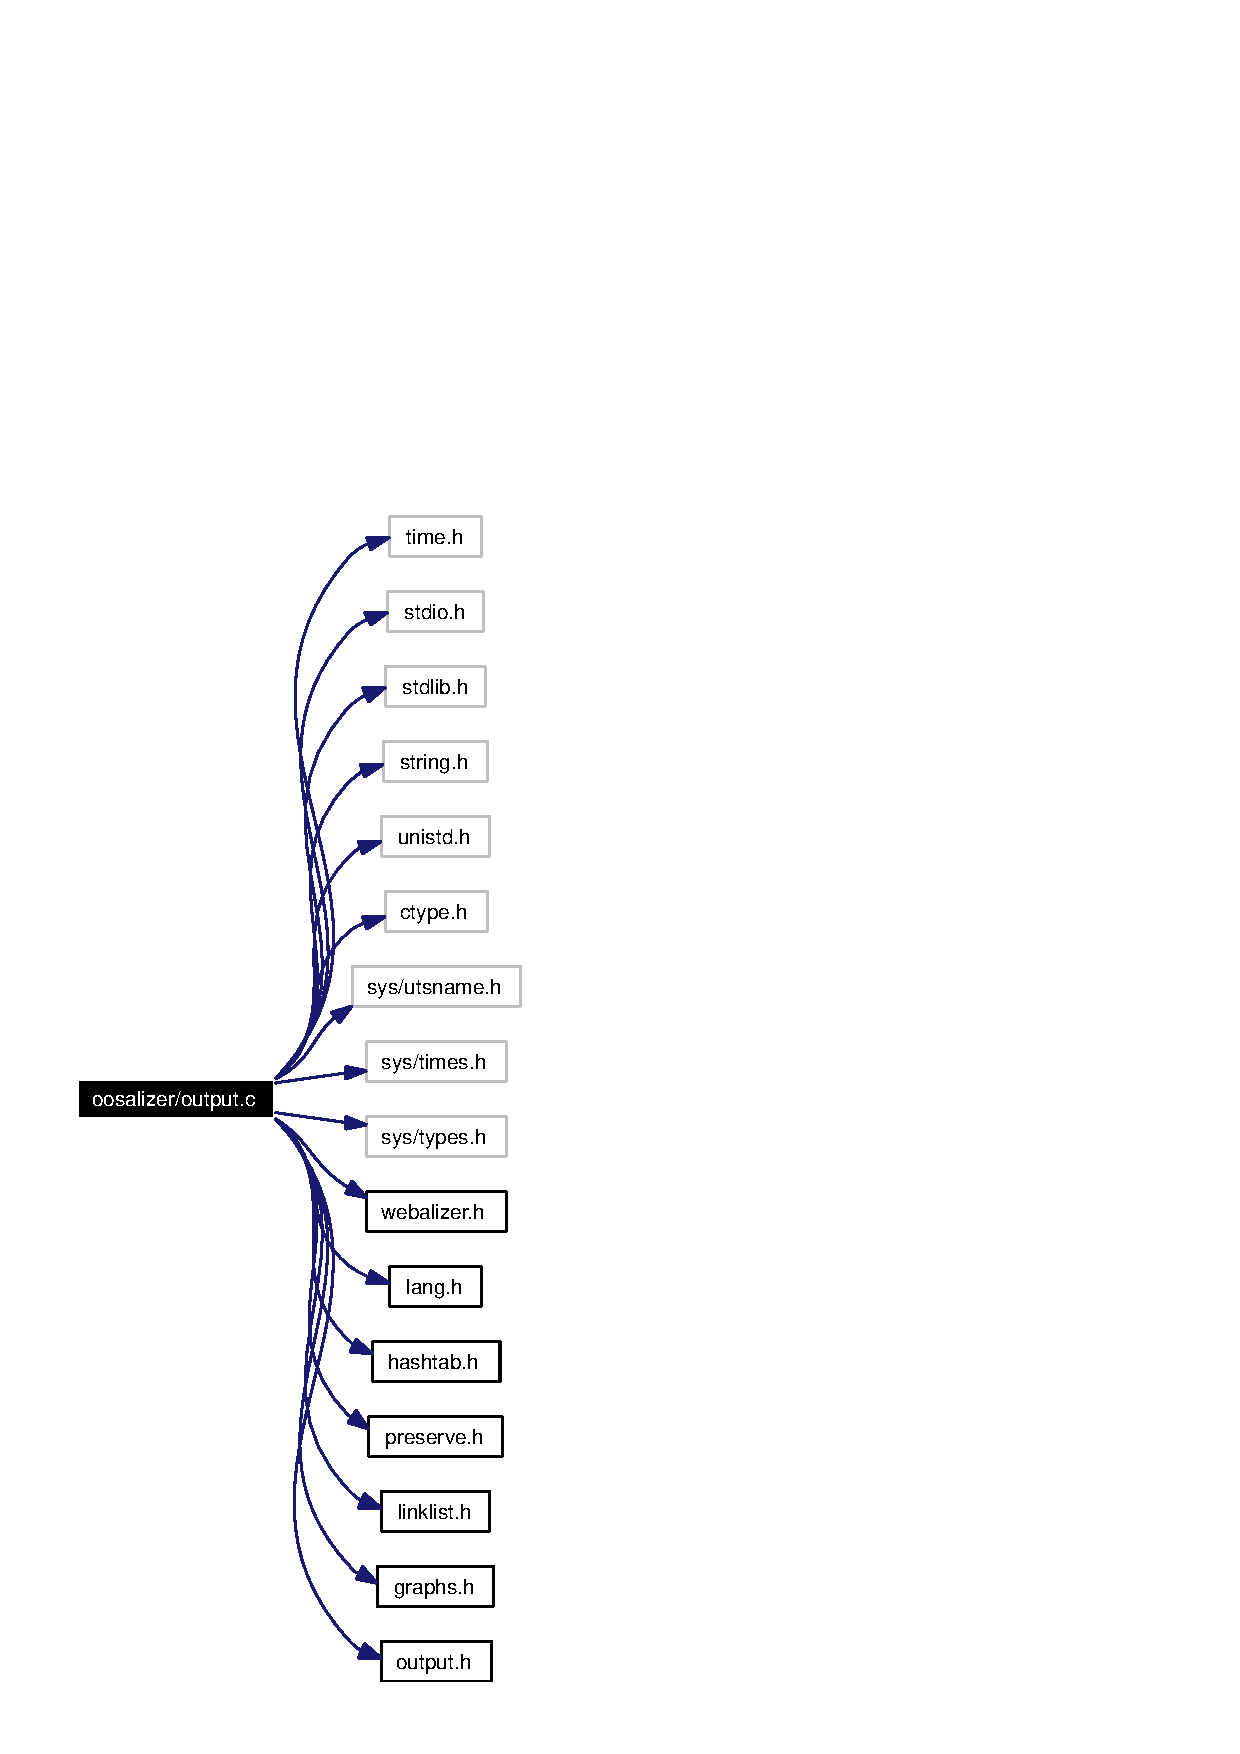
\includegraphics[width=125pt]{output_8c__incl}
\end{center}
\end{figure}
\subsection*{Makrodefinitionen}
\begin{CompactItemize}
\item 
\#define {\bf CLK\_\-TCK}~\_\-SC\_\-CLK\_\-TCK
\item 
\#define {\bf WHITE}~\char`\"{}\#FFFFFF\char`\"{}
\item 
\#define {\bf BLACK}~\char`\"{}\#000000\char`\"{}
\item 
\#define {\bf RED}~\char`\"{}\#FF0000\char`\"{}
\item 
\#define {\bf ORANGE}~\char`\"{}\#FF8000\char`\"{}
\item 
\#define {\bf LTBLUE}~\char`\"{}\#0080FF\char`\"{}
\item 
\#define {\bf BLUE}~\char`\"{}\#0000FF\char`\"{}
\item 
\#define {\bf GREEN}~\char`\"{}\#00FF00\char`\"{}
\item 
\#define {\bf DKGREEN}~\char`\"{}\#008040\char`\"{}
\item 
\#define {\bf GREY}~\char`\"{}\#C0C0C0\char`\"{}
\item 
\#define {\bf LTGREY}~\char`\"{}\#E8E8E8\char`\"{}
\item 
\#define {\bf YELLOW}~\char`\"{}\#FFFF00\char`\"{}
\item 
\#define {\bf PURPLE}~\char`\"{}\#FF00FF\char`\"{}
\item 
\#define {\bf CYAN}~\char`\"{}\#00E0FF\char`\"{}
\item 
\#define {\bf GRPCOLOR}~\char`\"{}\#D0D0E0\char`\"{}
\end{CompactItemize}
\subsection*{Funktionen}
\begin{CompactItemize}
\item 
void {\bf write\_\-html\_\-head} (char $\ast$, FILE $\ast$)
\item 
void {\bf write\_\-html\_\-tail} (FILE $\ast$)
\item 
void {\bf month\_\-links} ()
\item 
void {\bf month\_\-total\_\-table} ()
\item 
void {\bf month\_\-error\_\-table} ()
\item 
void {\bf daily\_\-total\_\-table} ()
\item 
void {\bf hourly\_\-total\_\-table} ()
\item 
void {\bf top\_\-sites\_\-table} (int)
\item 
void {\bf top\_\-urls\_\-table} (int)
\item 
void {\bf top\_\-entry\_\-table} (int)
\item 
void {\bf top\_\-refs\_\-table} ()
\item 
void {\bf top\_\-agents\_\-table} ()
\item 
void {\bf top\_\-ctry\_\-table} ()
\item 
void {\bf top\_\-search\_\-table} ()
\item 
void {\bf top\_\-users\_\-table} ()
\item 
u\_\-long {\bf load\_\-url\_\-array} ({\bf UNODEPTR} $\ast$)
\item 
u\_\-long {\bf load\_\-site\_\-array} ({\bf HNODEPTR} $\ast$)
\item 
u\_\-long {\bf load\_\-ref\_\-array} ({\bf RNODEPTR} $\ast$)
\item 
u\_\-long {\bf load\_\-agent\_\-array} ({\bf ANODEPTR} $\ast$)
\item 
u\_\-long {\bf load\_\-srch\_\-array} ({\bf SNODEPTR} $\ast$)
\item 
u\_\-long {\bf load\_\-ident\_\-array} ({\bf INODEPTR} $\ast$)
\item 
int {\bf qs\_\-url\_\-cmph} (const void $\ast$, const void $\ast$)
\item 
int {\bf qs\_\-url\_\-cmpk} (const void $\ast$, const void $\ast$)
\item 
int {\bf qs\_\-url\_\-cmpn} (const void $\ast$, const void $\ast$)
\item 
int {\bf qs\_\-url\_\-cmpx} (const void $\ast$, const void $\ast$)
\item 
int {\bf qs\_\-site\_\-cmph} (const void $\ast$, const void $\ast$)
\item 
int {\bf qs\_\-site\_\-cmpk} (const void $\ast$, const void $\ast$)
\item 
int {\bf qs\_\-ref\_\-cmph} (const void $\ast$, const void $\ast$)
\item 
int {\bf qs\_\-agnt\_\-cmph} (const void $\ast$, const void $\ast$)
\item 
int {\bf qs\_\-srch\_\-cmph} (const void $\ast$, const void $\ast$)
\item 
int {\bf qs\_\-ident\_\-cmph} (const void $\ast$, const void $\ast$)
\item 
int {\bf qs\_\-ident\_\-cmpk} (const void $\ast$, const void $\ast$)
\item 
int {\bf all\_\-sites\_\-page} (u\_\-long, u\_\-long)
\item 
int {\bf all\_\-urls\_\-page} (u\_\-long, u\_\-long)
\item 
int {\bf all\_\-refs\_\-page} (u\_\-long, u\_\-long)
\item 
int {\bf all\_\-agents\_\-page} (u\_\-long, u\_\-long)
\item 
int {\bf all\_\-search\_\-page} (u\_\-long, u\_\-long)
\item 
int {\bf all\_\-users\_\-page} (u\_\-long, u\_\-long)
\item 
void {\bf dump\_\-all\_\-sites} ()
\item 
void {\bf dump\_\-all\_\-urls} ()
\item 
void {\bf dump\_\-all\_\-refs} ()
\item 
void {\bf dump\_\-all\_\-agents} ()
\item 
void {\bf dump\_\-all\_\-users} ()
\item 
void {\bf dump\_\-all\_\-search} ()
\item 
int {\bf write\_\-month\_\-html} ()
\item 
int {\bf write\_\-main\_\-index} ()
\item 
FILE $\ast$ {\bf open\_\-out\_\-file} (char $\ast$filename)
\end{CompactItemize}
\subsection*{Variablen}
\begin{CompactItemize}
\item 
{\bf UNODEPTR} $\ast$ {\bf u\_\-array} = NULL
\item 
{\bf HNODEPTR} $\ast$ {\bf h\_\-array} = NULL
\item 
{\bf RNODEPTR} $\ast$ {\bf r\_\-array} = NULL
\item 
{\bf ANODEPTR} $\ast$ {\bf a\_\-array} = NULL
\item 
{\bf SNODEPTR} $\ast$ {\bf s\_\-array} = NULL
\item 
{\bf INODEPTR} $\ast$ {\bf i\_\-array} = NULL
\item 
u\_\-long {\bf a\_\-ctr} = 0
\item 
FILE $\ast$ {\bf out\_\-fp}
\end{CompactItemize}


\subsection{Makro-Dokumentation}
\index{output.c@{output.c}!BLACK@{BLACK}}
\index{BLACK@{BLACK}!output.c@{output.c}}
\subsubsection{\setlength{\rightskip}{0pt plus 5cm}\#define BLACK~\char`\"{}\#000000\char`\"{}}\label{output_8c_7b3b25cba33b07c303f3060fe41887f6}




Definiert in Zeile 119 der Datei output.c.

Wird benutzt von write\_\-html\_\-head().\index{output.c@{output.c}!BLUE@{BLUE}}
\index{BLUE@{BLUE}!output.c@{output.c}}
\subsubsection{\setlength{\rightskip}{0pt plus 5cm}\#define BLUE~\char`\"{}\#0000FF\char`\"{}}\label{output_8c_79d10e672abb49ad63eeaa8aaef57c38}




Definiert in Zeile 123 der Datei output.c.

Wird benutzt von write\_\-html\_\-head().\index{output.c@{output.c}!CLK_TCK@{CLK\_\-TCK}}
\index{CLK_TCK@{CLK\_\-TCK}!output.c@{output.c}}
\subsubsection{\setlength{\rightskip}{0pt plus 5cm}\#define CLK\_\-TCK~\_\-SC\_\-CLK\_\-TCK}\label{output_8c_03df76d1f70664d745ca8de2864e39b3}




Definiert in Zeile 59 der Datei output.c.\index{output.c@{output.c}!CYAN@{CYAN}}
\index{CYAN@{CYAN}!output.c@{output.c}}
\subsubsection{\setlength{\rightskip}{0pt plus 5cm}\#define CYAN~\char`\"{}\#00E0FF\char`\"{}}\label{output_8c_d243f93c16bc4c1d3e0a13b84421d760}




Definiert in Zeile 130 der Datei output.c.

Wird benutzt von daily\_\-total\_\-table(), hourly\_\-total\_\-table(), top\_\-agents\_\-table(), top\_\-entry\_\-table(), top\_\-refs\_\-table(), top\_\-search\_\-table(), top\_\-sites\_\-table(), top\_\-urls\_\-table() und top\_\-users\_\-table().\index{output.c@{output.c}!DKGREEN@{DKGREEN}}
\index{DKGREEN@{DKGREEN}!output.c@{output.c}}
\subsubsection{\setlength{\rightskip}{0pt plus 5cm}\#define DKGREEN~\char`\"{}\#008040\char`\"{}}\label{output_8c_70a867a7d5bd5ff0aa67003c99b93a8f}




Definiert in Zeile 125 der Datei output.c.

Wird benutzt von daily\_\-total\_\-table(), hourly\_\-total\_\-table(), top\_\-agents\_\-table(), top\_\-entry\_\-table(), top\_\-refs\_\-table(), top\_\-search\_\-table(), top\_\-sites\_\-table(), top\_\-urls\_\-table() und top\_\-users\_\-table().\index{output.c@{output.c}!GREEN@{GREEN}}
\index{GREEN@{GREEN}!output.c@{output.c}}
\subsubsection{\setlength{\rightskip}{0pt plus 5cm}\#define GREEN~\char`\"{}\#00FF00\char`\"{}}\label{output_8c_cfbc006ea433ad708fdee3e82996e721}




Definiert in Zeile 124 der Datei output.c.\index{output.c@{output.c}!GREY@{GREY}}
\index{GREY@{GREY}!output.c@{output.c}}
\subsubsection{\setlength{\rightskip}{0pt plus 5cm}\#define GREY~\char`\"{}\#C0C0C0\char`\"{}}\label{output_8c_dce122f566c88a1eceeb79a635afa964}




Definiert in Zeile 126 der Datei output.c.

Wird benutzt von daily\_\-total\_\-table(), hourly\_\-total\_\-table(), top\_\-agents\_\-table(), top\_\-entry\_\-table(), top\_\-refs\_\-table(), top\_\-search\_\-table(), top\_\-sites\_\-table(), top\_\-urls\_\-table() und top\_\-users\_\-table().\index{output.c@{output.c}!GRPCOLOR@{GRPCOLOR}}
\index{GRPCOLOR@{GRPCOLOR}!output.c@{output.c}}
\subsubsection{\setlength{\rightskip}{0pt plus 5cm}\#define GRPCOLOR~\char`\"{}\#D0D0E0\char`\"{}}\label{output_8c_d3d0166d909c5f2c8461b42d87f1f778}




Definiert in Zeile 131 der Datei output.c.

Wird benutzt von top\_\-agents\_\-table(), top\_\-refs\_\-table(), top\_\-search\_\-table(), top\_\-sites\_\-table(), top\_\-urls\_\-table() und top\_\-users\_\-table().\index{output.c@{output.c}!LTBLUE@{LTBLUE}}
\index{LTBLUE@{LTBLUE}!output.c@{output.c}}
\subsubsection{\setlength{\rightskip}{0pt plus 5cm}\#define LTBLUE~\char`\"{}\#0080FF\char`\"{}}\label{output_8c_1a13e2f5e41385c6b4ce64b8b683e5d2}




Definiert in Zeile 122 der Datei output.c.

Wird benutzt von daily\_\-total\_\-table(), hourly\_\-total\_\-table(), top\_\-sites\_\-table() und top\_\-users\_\-table().\index{output.c@{output.c}!LTGREY@{LTGREY}}
\index{LTGREY@{LTGREY}!output.c@{output.c}}
\subsubsection{\setlength{\rightskip}{0pt plus 5cm}\#define LTGREY~\char`\"{}\#E8E8E8\char`\"{}}\label{output_8c_0ffe2221c8690dc80b5f9553474dd096}




Definiert in Zeile 127 der Datei output.c.

Wird benutzt von write\_\-html\_\-head().\index{output.c@{output.c}!ORANGE@{ORANGE}}
\index{ORANGE@{ORANGE}!output.c@{output.c}}
\subsubsection{\setlength{\rightskip}{0pt plus 5cm}\#define ORANGE~\char`\"{}\#FF8000\char`\"{}}\label{output_8c_c5b6e19bf06822021f35602c59658de3}




Definiert in Zeile 121 der Datei output.c.

Wird benutzt von daily\_\-total\_\-table().\index{output.c@{output.c}!PURPLE@{PURPLE}}
\index{PURPLE@{PURPLE}!output.c@{output.c}}
\subsubsection{\setlength{\rightskip}{0pt plus 5cm}\#define PURPLE~\char`\"{}\#FF00FF\char`\"{}}\label{output_8c_0bb0b009e7a7390473ace4d98bd843c0}




Definiert in Zeile 129 der Datei output.c.\index{output.c@{output.c}!RED@{RED}}
\index{RED@{RED}!output.c@{output.c}}
\subsubsection{\setlength{\rightskip}{0pt plus 5cm}\#define RED~\char`\"{}\#FF0000\char`\"{}}\label{output_8c_8d23feea868a983c8c2b661e1e16972f}




Definiert in Zeile 120 der Datei output.c.

Wird benutzt von daily\_\-total\_\-table(), hourly\_\-total\_\-table(), top\_\-sites\_\-table(), top\_\-urls\_\-table(), top\_\-users\_\-table() und write\_\-html\_\-head().\index{output.c@{output.c}!WHITE@{WHITE}}
\index{WHITE@{WHITE}!output.c@{output.c}}
\subsubsection{\setlength{\rightskip}{0pt plus 5cm}\#define WHITE~\char`\"{}\#FFFFFF\char`\"{}}\label{output_8c_87b537f5fa5c109d3c05c13d6b18f382}




Definiert in Zeile 118 der Datei output.c.\index{output.c@{output.c}!YELLOW@{YELLOW}}
\index{YELLOW@{YELLOW}!output.c@{output.c}}
\subsubsection{\setlength{\rightskip}{0pt plus 5cm}\#define YELLOW~\char`\"{}\#FFFF00\char`\"{}}\label{output_8c_bf681265909adf3d3e8116c93c0ba179}




Definiert in Zeile 128 der Datei output.c.

Wird benutzt von daily\_\-total\_\-table(), top\_\-entry\_\-table(), top\_\-sites\_\-table() und top\_\-users\_\-table().

\subsection{Dokumentation der Funktionen}
\index{output.c@{output.c}!all_agents_page@{all\_\-agents\_\-page}}
\index{all_agents_page@{all\_\-agents\_\-page}!output.c@{output.c}}
\subsubsection{\setlength{\rightskip}{0pt plus 5cm}int all\_\-agents\_\-page (u\_\-long, u\_\-long)}\label{output_8c_4f27932d464425450d0c11106ae0c2fe}




Definiert in Zeile 1713 der Datei output.c.

Benutzt a\_\-array, buffer, anode::count, cur\_\-month, cur\_\-year, anode::flag, html\_\-ext, l\_\-month, msg\_\-h\_\-agent, msg\_\-h\_\-hits, OBJ\_\-GRP, OBJ\_\-REG, open\_\-out\_\-file(), out\_\-fp, anode::string, t\_\-hit, write\_\-html\_\-head() und write\_\-html\_\-tail().

Wird benutzt von top\_\-agents\_\-table().\index{output.c@{output.c}!all_refs_page@{all\_\-refs\_\-page}}
\index{all_refs_page@{all\_\-refs\_\-page}!output.c@{output.c}}
\subsubsection{\setlength{\rightskip}{0pt plus 5cm}int all\_\-refs\_\-page (u\_\-long, u\_\-long)}\label{output_8c_ffa5d4248e6a8d3946f094e5a16c026e}




Definiert in Zeile 1561 der Datei output.c.

Benutzt buffer, rnode::count, cur\_\-month, cur\_\-year, rnode::flag, html\_\-ext, l\_\-month, msg\_\-h\_\-hits, msg\_\-h\_\-ref, OBJ\_\-GRP, OBJ\_\-REG, open\_\-out\_\-file(), out\_\-fp, r\_\-array, rnode::string, t\_\-hit, write\_\-html\_\-head() und write\_\-html\_\-tail().

Wird benutzt von top\_\-refs\_\-table().\index{output.c@{output.c}!all_search_page@{all\_\-search\_\-page}}
\index{all_search_page@{all\_\-search\_\-page}!output.c@{output.c}}
\subsubsection{\setlength{\rightskip}{0pt plus 5cm}int all\_\-search\_\-page (u\_\-long, u\_\-long)}\label{output_8c_b218b4268390f2e5c00ef1f303d3baad}




Definiert in Zeile 1846 der Datei output.c.

Benutzt buffer, snode::count, cur\_\-month, cur\_\-year, html\_\-ext, l\_\-month, msg\_\-h\_\-hits, msg\_\-h\_\-search, open\_\-out\_\-file(), out\_\-fp, s\_\-array, snode::string, write\_\-html\_\-head() und write\_\-html\_\-tail().

Wird benutzt von top\_\-search\_\-table().\index{output.c@{output.c}!all_sites_page@{all\_\-sites\_\-page}}
\index{all_sites_page@{all\_\-sites\_\-page}!output.c@{output.c}}
\subsubsection{\setlength{\rightskip}{0pt plus 5cm}int all\_\-sites\_\-page (u\_\-long, u\_\-long)}\label{output_8c_c4e6c9fc2562755c38403dd45bdab4e9}




Definiert in Zeile 1085 der Datei output.c.

Benutzt buffer, hnode::count, cur\_\-month, cur\_\-year, hnode::files, hnode::flag, h\_\-array, hide\_\-sites, html\_\-ext, l\_\-month, msg\_\-h\_\-files, msg\_\-h\_\-hits, msg\_\-h\_\-hname, msg\_\-h\_\-sites, msg\_\-h\_\-visits, msg\_\-h\_\-xfer, OBJ\_\-GRP, OBJ\_\-REG, open\_\-out\_\-file(), out\_\-fp, hnode::string, t\_\-file, t\_\-hit, t\_\-visit, t\_\-xfer, hnode::visit, write\_\-html\_\-head(), write\_\-html\_\-tail() und hnode::xfer.

Wird benutzt von top\_\-sites\_\-table().\index{output.c@{output.c}!all_urls_page@{all\_\-urls\_\-page}}
\index{all_urls_page@{all\_\-urls\_\-page}!output.c@{output.c}}
\subsubsection{\setlength{\rightskip}{0pt plus 5cm}int all\_\-urls\_\-page (u\_\-long, u\_\-long)}\label{output_8c_510367124c184f22aac1331c1412c7d5}




Definiert in Zeile 1290 der Datei output.c.

Benutzt buffer, unode::count, cur\_\-month, cur\_\-year, unode::flag, html\_\-ext, l\_\-month, msg\_\-h\_\-hits, msg\_\-h\_\-url, msg\_\-h\_\-xfer, OBJ\_\-GRP, OBJ\_\-REG, open\_\-out\_\-file(), out\_\-fp, unode::string, t\_\-hit, t\_\-xfer, u\_\-array, write\_\-html\_\-head(), write\_\-html\_\-tail() und unode::xfer.

Wird benutzt von top\_\-urls\_\-table().\index{output.c@{output.c}!all_users_page@{all\_\-users\_\-page}}
\index{all_users_page@{all\_\-users\_\-page}!output.c@{output.c}}
\subsubsection{\setlength{\rightskip}{0pt plus 5cm}int all\_\-users\_\-page (u\_\-long, u\_\-long)}\label{output_8c_b1313f0c59efbacd626ea5fb185f126e}




Definiert in Zeile 1990 der Datei output.c.

Benutzt buffer, inode::count, cur\_\-month, cur\_\-year, inode::files, inode::flag, html\_\-ext, i\_\-array, l\_\-month, msg\_\-h\_\-files, msg\_\-h\_\-hits, msg\_\-h\_\-uname, msg\_\-h\_\-visits, msg\_\-h\_\-xfer, OBJ\_\-GRP, OBJ\_\-REG, open\_\-out\_\-file(), out\_\-fp, inode::string, t\_\-file, t\_\-hit, t\_\-visit, t\_\-xfer, inode::visit, write\_\-html\_\-head(), write\_\-html\_\-tail() und inode::xfer.

Wird benutzt von top\_\-users\_\-table().\index{output.c@{output.c}!daily_total_table@{daily\_\-total\_\-table}}
\index{daily_total_table@{daily\_\-total\_\-table}!output.c@{output.c}}
\subsubsection{\setlength{\rightskip}{0pt plus 5cm}void daily\_\-total\_\-table ()}\label{output_8c_24968f52f4cb828c450b4357d0da9326}




Definiert in Zeile 804 der Datei output.c.

Benutzt cur\_\-month, cur\_\-year, CYAN, DKGREEN, GREY, hist\_\-lday, l\_\-month, LTBLUE, msg\_\-dtot\_\-ds, msg\_\-h\_\-day, msg\_\-h\_\-files, msg\_\-h\_\-hits, msg\_\-h\_\-pages, msg\_\-h\_\-sites, msg\_\-h\_\-visits, msg\_\-h\_\-xfer, ORANGE, out\_\-fp, PCENT, RED, t\_\-file, t\_\-hit, t\_\-page, t\_\-site, t\_\-visit, t\_\-xfer, tm\_\-file, tm\_\-hit, tm\_\-page, tm\_\-site, tm\_\-visit, tm\_\-xfer und YELLOW.

Wird benutzt von write\_\-month\_\-html().\index{output.c@{output.c}!dump_all_agents@{dump\_\-all\_\-agents}}
\index{dump_all_agents@{dump\_\-all\_\-agents}!output.c@{output.c}}
\subsubsection{\setlength{\rightskip}{0pt plus 5cm}void dump\_\-all\_\-agents ()}\label{output_8c_13b9a7e783dc0408ef406d95e9a347a8}




Definiert in Zeile 2332 der Datei output.c.

Benutzt a\_\-array, a\_\-ctr, anode::count, cur\_\-month, cur\_\-year, dump\_\-ext, dump\_\-header, dump\_\-path, anode::flag, msg\_\-h\_\-agent, msg\_\-h\_\-hits, OBJ\_\-GRP, open\_\-out\_\-file(), out\_\-fp und anode::string.

Wird benutzt von write\_\-month\_\-html().\index{output.c@{output.c}!dump_all_refs@{dump\_\-all\_\-refs}}
\index{dump_all_refs@{dump\_\-all\_\-refs}!output.c@{output.c}}
\subsubsection{\setlength{\rightskip}{0pt plus 5cm}void dump\_\-all\_\-refs ()}\label{output_8c_246f33aca4a4783b5b9853d70aa44d61}




Definiert in Zeile 2293 der Datei output.c.

Benutzt a\_\-ctr, rnode::count, cur\_\-month, cur\_\-year, dump\_\-ext, dump\_\-header, dump\_\-path, rnode::flag, msg\_\-h\_\-hits, msg\_\-h\_\-ref, OBJ\_\-GRP, open\_\-out\_\-file(), out\_\-fp, r\_\-array und rnode::string.

Wird benutzt von write\_\-month\_\-html().\index{output.c@{output.c}!dump_all_search@{dump\_\-all\_\-search}}
\index{dump_all_search@{dump\_\-all\_\-search}!output.c@{output.c}}
\subsubsection{\setlength{\rightskip}{0pt plus 5cm}void dump\_\-all\_\-search ()}\label{output_8c_46280cc9688bd8a784859589d0ca588e}




Definiert in Zeile 2414 der Datei output.c.

Benutzt a\_\-ctr, snode::count, cur\_\-month, cur\_\-year, dump\_\-ext, dump\_\-header, dump\_\-path, msg\_\-h\_\-hits, msg\_\-h\_\-search, open\_\-out\_\-file(), out\_\-fp, s\_\-array und snode::string.

Wird benutzt von write\_\-month\_\-html().\index{output.c@{output.c}!dump_all_sites@{dump\_\-all\_\-sites}}
\index{dump_all_sites@{dump\_\-all\_\-sites}!output.c@{output.c}}
\subsubsection{\setlength{\rightskip}{0pt plus 5cm}void dump\_\-all\_\-sites ()}\label{output_8c_1ff4091dce5e22d1f8f4cc034a78afec}




Definiert in Zeile 2210 der Datei output.c.

Benutzt a\_\-ctr, hnode::count, cur\_\-month, cur\_\-year, dump\_\-ext, dump\_\-header, dump\_\-path, hnode::files, hnode::flag, h\_\-array, msg\_\-h\_\-files, msg\_\-h\_\-hits, msg\_\-h\_\-hname, msg\_\-h\_\-visits, msg\_\-h\_\-xfer, OBJ\_\-GRP, open\_\-out\_\-file(), out\_\-fp, hnode::string, hnode::visit und hnode::xfer.

Wird benutzt von write\_\-month\_\-html().\index{output.c@{output.c}!dump_all_urls@{dump\_\-all\_\-urls}}
\index{dump_all_urls@{dump\_\-all\_\-urls}!output.c@{output.c}}
\subsubsection{\setlength{\rightskip}{0pt plus 5cm}void dump\_\-all\_\-urls ()}\label{output_8c_d1bfd511fab3836f3e1d1867384b425f}




Definiert in Zeile 2253 der Datei output.c.

Benutzt a\_\-ctr, unode::count, cur\_\-month, cur\_\-year, dump\_\-ext, dump\_\-header, dump\_\-path, unode::flag, msg\_\-h\_\-hits, msg\_\-h\_\-url, msg\_\-h\_\-xfer, OBJ\_\-GRP, open\_\-out\_\-file(), out\_\-fp, unode::string, u\_\-array und unode::xfer.

Wird benutzt von write\_\-month\_\-html().\index{output.c@{output.c}!dump_all_users@{dump\_\-all\_\-users}}
\index{dump_all_users@{dump\_\-all\_\-users}!output.c@{output.c}}
\subsubsection{\setlength{\rightskip}{0pt plus 5cm}void dump\_\-all\_\-users ()}\label{output_8c_a519e8d866cad7c01f72636d749a9f57}




Definiert in Zeile 2371 der Datei output.c.

Benutzt a\_\-ctr, inode::count, cur\_\-month, cur\_\-year, dump\_\-ext, dump\_\-header, dump\_\-path, inode::files, inode::flag, i\_\-array, msg\_\-h\_\-files, msg\_\-h\_\-hits, msg\_\-h\_\-uname, msg\_\-h\_\-visits, msg\_\-h\_\-xfer, OBJ\_\-GRP, open\_\-out\_\-file(), out\_\-fp, inode::string, inode::visit und inode::xfer.

Wird benutzt von write\_\-month\_\-html().\index{output.c@{output.c}!hourly_total_table@{hourly\_\-total\_\-table}}
\index{hourly_total_table@{hourly\_\-total\_\-table}!output.c@{output.c}}
\subsubsection{\setlength{\rightskip}{0pt plus 5cm}void hourly\_\-total\_\-table ()}\label{output_8c_bed9fdc7ecf13c9399e3e41bd583abd9}




Definiert in Zeile 881 der Datei output.c.

Benutzt cur\_\-month, cur\_\-year, CYAN, DKGREEN, f\_\-day, GREY, l\_\-day, l\_\-month, LTBLUE, msg\_\-h\_\-avg, msg\_\-h\_\-files, msg\_\-h\_\-hits, msg\_\-h\_\-hour, msg\_\-h\_\-pages, msg\_\-h\_\-total, msg\_\-h\_\-xfer, msg\_\-htot\_\-hs, out\_\-fp, PCENT, RED, t\_\-file, t\_\-hit, t\_\-page, t\_\-xfer, th\_\-file, th\_\-hit, th\_\-page und th\_\-xfer.

Wird benutzt von write\_\-month\_\-html().\index{output.c@{output.c}!load_agent_array@{load\_\-agent\_\-array}}
\index{load_agent_array@{load\_\-agent\_\-array}!output.c@{output.c}}
\subsubsection{\setlength{\rightskip}{0pt plus 5cm}u\_\-long load\_\-agent\_\-array ({\bf ANODEPTR} $\ast$)}\label{output_8c_695c31f8c5d53bf9a1b112cccd36740f}




Definiert in Zeile 2819 der Datei output.c.

Benutzt am\_\-htab, MAXHASH und anode::next.

Wird benutzt von write\_\-month\_\-html().\index{output.c@{output.c}!load_ident_array@{load\_\-ident\_\-array}}
\index{load_ident_array@{load\_\-ident\_\-array}!output.c@{output.c}}
\subsubsection{\setlength{\rightskip}{0pt plus 5cm}u\_\-long load\_\-ident\_\-array ({\bf INODEPTR} $\ast$)}\label{output_8c_78caf44e7545035a80e85f498cb9e471}




Definiert in Zeile 2867 der Datei output.c.

Benutzt im\_\-htab, MAXHASH und inode::next.

Wird benutzt von write\_\-month\_\-html().\index{output.c@{output.c}!load_ref_array@{load\_\-ref\_\-array}}
\index{load_ref_array@{load\_\-ref\_\-array}!output.c@{output.c}}
\subsubsection{\setlength{\rightskip}{0pt plus 5cm}u\_\-long load\_\-ref\_\-array ({\bf RNODEPTR} $\ast$)}\label{output_8c_4fe67ad14b790d3dabec4fc028e338c5}




Definiert in Zeile 2795 der Datei output.c.

Benutzt MAXHASH, rnode::next und rm\_\-htab.

Wird benutzt von write\_\-month\_\-html().\index{output.c@{output.c}!load_site_array@{load\_\-site\_\-array}}
\index{load_site_array@{load\_\-site\_\-array}!output.c@{output.c}}
\subsubsection{\setlength{\rightskip}{0pt plus 5cm}u\_\-long load\_\-site\_\-array ({\bf HNODEPTR} $\ast$)}\label{output_8c_12790ed69b92f9024071f8e8ba312ee3}




Definiert in Zeile 2747 der Datei output.c.

Benutzt MAXHASH, hnode::next und sm\_\-htab.

Wird benutzt von write\_\-month\_\-html().\index{output.c@{output.c}!load_srch_array@{load\_\-srch\_\-array}}
\index{load_srch_array@{load\_\-srch\_\-array}!output.c@{output.c}}
\subsubsection{\setlength{\rightskip}{0pt plus 5cm}u\_\-long load\_\-srch\_\-array ({\bf SNODEPTR} $\ast$)}\label{output_8c_d3eb19f2c468e374066739cccec7d3d4}




Definiert in Zeile 2843 der Datei output.c.

Benutzt MAXHASH, snode::next und sr\_\-htab.

Wird benutzt von write\_\-month\_\-html().\index{output.c@{output.c}!load_url_array@{load\_\-url\_\-array}}
\index{load_url_array@{load\_\-url\_\-array}!output.c@{output.c}}
\subsubsection{\setlength{\rightskip}{0pt plus 5cm}u\_\-long load\_\-url\_\-array ({\bf UNODEPTR} $\ast$)}\label{output_8c_0d5c8398a3b959aa372077fda3f78fff}




Definiert in Zeile 2771 der Datei output.c.

Benutzt MAXHASH, unode::next und um\_\-htab.

Wird benutzt von write\_\-month\_\-html().\index{output.c@{output.c}!month_error_table@{month\_\-error\_\-table}}
\index{month_error_table@{month\_\-error\_\-table}!output.c@{output.c}}
\subsubsection{\setlength{\rightskip}{0pt plus 5cm}void month\_\-error\_\-table ()}\label{output_8c_267f41fceee149a1e7eeb4ee30ee5f09}




Definiert in Zeile 715 der Datei output.c.

Benutzt response\_\-url::count, responsetmp\_\-url::count, resp\_\-counter, respnotfound, respnotfoundtmp, response\_\-url::respurl und responsetmp\_\-url::respurl.

Wird benutzt von write\_\-month\_\-html().\index{output.c@{output.c}!month_links@{month\_\-links}}
\index{month_links@{month\_\-links}!output.c@{output.c}}
\subsubsection{\setlength{\rightskip}{0pt plus 5cm}void month\_\-links ()}\label{output_8c_88fc4fa78dab50f356e5daebd1c0efcb}




Definiert in Zeile 537 der Datei output.c.

Benutzt daily\_\-graph, daily\_\-stats, hourly\_\-graph, hourly\_\-stats, msg\_\-hlnk\_\-a, msg\_\-hlnk\_\-c, msg\_\-hlnk\_\-ds, msg\_\-hlnk\_\-en, msg\_\-hlnk\_\-ex, msg\_\-hlnk\_\-hs, msg\_\-hlnk\_\-i, msg\_\-hlnk\_\-r, msg\_\-hlnk\_\-s, msg\_\-hlnk\_\-sr, msg\_\-hlnk\_\-u, ntop\_\-agents, ntop\_\-ctrys, ntop\_\-entry, ntop\_\-exit, ntop\_\-notfound, ntop\_\-refs, ntop\_\-search, ntop\_\-sites, ntop\_\-sites\-K, ntop\_\-urls, ntop\_\-urls\-K, ntop\_\-users, out\_\-fp, response, t\_\-agent, t\_\-ref und t\_\-user.

Wird benutzt von write\_\-month\_\-html().\index{output.c@{output.c}!month_total_table@{month\_\-total\_\-table}}
\index{month_total_table@{month\_\-total\_\-table}!output.c@{output.c}}
\subsubsection{\setlength{\rightskip}{0pt plus 5cm}void month\_\-total\_\-table ()}\label{output_8c_f2c834f471b87d6264d3694c8257382c}




Definiert in Zeile 571 der Datei output.c.

Benutzt f\_\-day, l\_\-day, tm\_\-file, tm\_\-hit, tm\_\-page, tm\_\-visit und tm\_\-xfer.

Wird benutzt von write\_\-month\_\-html().\index{output.c@{output.c}!open_out_file@{open\_\-out\_\-file}}
\index{open_out_file@{open\_\-out\_\-file}!output.c@{output.c}}
\subsubsection{\setlength{\rightskip}{0pt plus 5cm}FILE$\ast$ open\_\-out\_\-file (char $\ast$ {\em filename})}\label{output_8c_837e8afa754fafe8bf3e4e71da7db321}




Definiert in Zeile 2891 der Datei output.c.

Benutzt msg\_\-no\_\-open, out\_\-fp und verbose.

Wird benutzt von all\_\-agents\_\-page(), all\_\-refs\_\-page(), all\_\-search\_\-page(), all\_\-sites\_\-page(), all\_\-urls\_\-page(), all\_\-users\_\-page(), dump\_\-all\_\-agents(), dump\_\-all\_\-refs(), dump\_\-all\_\-search(), dump\_\-all\_\-sites(), dump\_\-all\_\-urls(), dump\_\-all\_\-users() und write\_\-month\_\-html().\index{output.c@{output.c}!qs_agnt_cmph@{qs\_\-agnt\_\-cmph}}
\index{qs_agnt_cmph@{qs\_\-agnt\_\-cmph}!output.c@{output.c}}
\subsubsection{\setlength{\rightskip}{0pt plus 5cm}int qs\_\-agnt\_\-cmph (const void $\ast$, const void $\ast$)}\label{output_8c_72a92b6a4155e75b035247485efacd27}




Definiert in Zeile 2702 der Datei output.c.

Wird benutzt von write\_\-month\_\-html().\index{output.c@{output.c}!qs_ident_cmph@{qs\_\-ident\_\-cmph}}
\index{qs_ident_cmph@{qs\_\-ident\_\-cmph}!output.c@{output.c}}
\subsubsection{\setlength{\rightskip}{0pt plus 5cm}int qs\_\-ident\_\-cmph (const void $\ast$, const void $\ast$)}\label{output_8c_ab10c25bdfd5abd8dda51817fa9027cd}




Definiert in Zeile 2732 der Datei output.c.

Wird benutzt von write\_\-month\_\-html().\index{output.c@{output.c}!qs_ident_cmpk@{qs\_\-ident\_\-cmpk}}
\index{qs_ident_cmpk@{qs\_\-ident\_\-cmpk}!output.c@{output.c}}
\subsubsection{\setlength{\rightskip}{0pt plus 5cm}int qs\_\-ident\_\-cmpk (const void $\ast$, const void $\ast$)}\label{output_8c_629673e2af2406711232e87efa863b16}


\index{output.c@{output.c}!qs_ref_cmph@{qs\_\-ref\_\-cmph}}
\index{qs_ref_cmph@{qs\_\-ref\_\-cmph}!output.c@{output.c}}
\subsubsection{\setlength{\rightskip}{0pt plus 5cm}int qs\_\-ref\_\-cmph (const void $\ast$, const void $\ast$)}\label{output_8c_9fcda824a6cb67eea93f6c873ce382e2}




Definiert in Zeile 2687 der Datei output.c.

Wird benutzt von write\_\-month\_\-html().\index{output.c@{output.c}!qs_site_cmph@{qs\_\-site\_\-cmph}}
\index{qs_site_cmph@{qs\_\-site\_\-cmph}!output.c@{output.c}}
\subsubsection{\setlength{\rightskip}{0pt plus 5cm}int qs\_\-site\_\-cmph (const void $\ast$, const void $\ast$)}\label{output_8c_322ce92d71bc2e3c8d61c5edfa937b66}




Definiert in Zeile 2597 der Datei output.c.

Wird benutzt von top\_\-sites\_\-table() und write\_\-month\_\-html().\index{output.c@{output.c}!qs_site_cmpk@{qs\_\-site\_\-cmpk}}
\index{qs_site_cmpk@{qs\_\-site\_\-cmpk}!output.c@{output.c}}
\subsubsection{\setlength{\rightskip}{0pt plus 5cm}int qs\_\-site\_\-cmpk (const void $\ast$, const void $\ast$)}\label{output_8c_0fe214a5ca06da7ea31019f2491f690f}




Definiert in Zeile 2612 der Datei output.c.

Wird benutzt von write\_\-month\_\-html().\index{output.c@{output.c}!qs_srch_cmph@{qs\_\-srch\_\-cmph}}
\index{qs_srch_cmph@{qs\_\-srch\_\-cmph}!output.c@{output.c}}
\subsubsection{\setlength{\rightskip}{0pt plus 5cm}int qs\_\-srch\_\-cmph (const void $\ast$, const void $\ast$)}\label{output_8c_c696a3022740c5d7e16758e13cd6240d}




Definiert in Zeile 2717 der Datei output.c.

Wird benutzt von write\_\-month\_\-html().\index{output.c@{output.c}!qs_url_cmph@{qs\_\-url\_\-cmph}}
\index{qs_url_cmph@{qs\_\-url\_\-cmph}!output.c@{output.c}}
\subsubsection{\setlength{\rightskip}{0pt plus 5cm}int qs\_\-url\_\-cmph (const void $\ast$, const void $\ast$)}\label{output_8c_aa5ed357df2c1098b3bf0d4fbbf020bb}




Definiert in Zeile 2627 der Datei output.c.

Wird benutzt von top\_\-urls\_\-table() und write\_\-month\_\-html().\index{output.c@{output.c}!qs_url_cmpk@{qs\_\-url\_\-cmpk}}
\index{qs_url_cmpk@{qs\_\-url\_\-cmpk}!output.c@{output.c}}
\subsubsection{\setlength{\rightskip}{0pt plus 5cm}int qs\_\-url\_\-cmpk (const void $\ast$, const void $\ast$)}\label{output_8c_ba53a184207ad59b18a510a690d29b5d}




Definiert in Zeile 2642 der Datei output.c.

Wird benutzt von write\_\-month\_\-html().\index{output.c@{output.c}!qs_url_cmpn@{qs\_\-url\_\-cmpn}}
\index{qs_url_cmpn@{qs\_\-url\_\-cmpn}!output.c@{output.c}}
\subsubsection{\setlength{\rightskip}{0pt plus 5cm}int qs\_\-url\_\-cmpn (const void $\ast$, const void $\ast$)}\label{output_8c_3b87c7768eed36e84a622e431b378942}




Definiert in Zeile 2657 der Datei output.c.

Wird benutzt von write\_\-month\_\-html().\index{output.c@{output.c}!qs_url_cmpx@{qs\_\-url\_\-cmpx}}
\index{qs_url_cmpx@{qs\_\-url\_\-cmpx}!output.c@{output.c}}
\subsubsection{\setlength{\rightskip}{0pt plus 5cm}int qs\_\-url\_\-cmpx (const void $\ast$, const void $\ast$)}\label{output_8c_9fb87dcc576463c9ce98593782734d59}




Definiert in Zeile 2672 der Datei output.c.

Wird benutzt von write\_\-month\_\-html().\index{output.c@{output.c}!top_agents_table@{top\_\-agents\_\-table}}
\index{top_agents_table@{top\_\-agents\_\-table}!output.c@{output.c}}
\subsubsection{\setlength{\rightskip}{0pt plus 5cm}void top\_\-agents\_\-table ()}\label{output_8c_55f5637d81e4b2847ea889ac14cbcc6b}




Definiert in Zeile 1623 der Datei output.c.

Benutzt a\_\-array, a\_\-ctr, all\_\-agents, all\_\-agents\_\-page(), anode::count, cur\_\-month, cur\_\-year, CYAN, DKGREEN, anode::flag, GREY, GRPCOLOR, hlite\_\-groups, html\_\-ext, msg\_\-h\_\-agent, msg\_\-h\_\-hits, msg\_\-top\_\-a, msg\_\-top\_\-of, msg\_\-top\_\-top, msg\_\-v\_\-agents, ntop\_\-agents, OBJ\_\-GRP, OBJ\_\-HIDE, OBJ\_\-REG, out\_\-fp, shade\_\-groups, anode::string, t\_\-agent und t\_\-hit.

Wird benutzt von write\_\-month\_\-html().\index{output.c@{output.c}!top_ctry_table@{top\_\-ctry\_\-table}}
\index{top_ctry_table@{top\_\-ctry\_\-table}!output.c@{output.c}}
\subsubsection{\setlength{\rightskip}{0pt plus 5cm}void top\_\-ctry\_\-table ()}\label{output_8c_c1ecb6ecbe9f7218b2e9ccae79cf2f5f}




Definiert in Zeile 2063 der Datei output.c.

Benutzt hnode::count, responsetmp\_\-url::count, ctry, ctry\_\-graph, hnode::files, country\_\-code::files, hnode::flag, MAXHASH, OBJ\_\-GRP, sm\_\-htab, hnode::string, hnode::xfer und country\_\-code::xfer.

Wird benutzt von write\_\-month\_\-html().\index{output.c@{output.c}!top_entry_table@{top\_\-entry\_\-table}}
\index{top_entry_table@{top\_\-entry\_\-table}!output.c@{output.c}}
\subsubsection{\setlength{\rightskip}{0pt plus 5cm}void top\_\-entry\_\-table (int)}\label{output_8c_72037da3c986417f62837bb8c96b60c0}




Definiert in Zeile 1359 der Datei output.c.

Benutzt a\_\-ctr, unode::count, CYAN, DKGREEN, unode::entry, unode::exit, unode::flag, GREY, hname, msg\_\-h\_\-hits, msg\_\-h\_\-url, msg\_\-h\_\-visits, msg\_\-top\_\-en, msg\_\-top\_\-ex, msg\_\-top\_\-of, msg\_\-top\_\-top, ntop\_\-entry, ntop\_\-exit, OBJ\_\-HIDE, OBJ\_\-REG, out\_\-fp, unode::string, t\_\-hit, u\_\-array, use\_\-https und YELLOW.

Wird benutzt von write\_\-month\_\-html().\index{output.c@{output.c}!top_refs_table@{top\_\-refs\_\-table}}
\index{top_refs_table@{top\_\-refs\_\-table}!output.c@{output.c}}
\subsubsection{\setlength{\rightskip}{0pt plus 5cm}void top\_\-refs\_\-table ()}\label{output_8c_f175d11f499a6782ad34c4b21f6891e1}




Definiert in Zeile 1461 der Datei output.c.

Benutzt a\_\-ctr, all\_\-refs, all\_\-refs\_\-page(), rnode::count, cur\_\-month, cur\_\-year, CYAN, DKGREEN, rnode::flag, GREY, GRPCOLOR, hlite\_\-groups, html\_\-ext, msg\_\-h\_\-hits, msg\_\-h\_\-ref, msg\_\-top\_\-of, msg\_\-top\_\-r, msg\_\-top\_\-top, msg\_\-v\_\-refs, ntop\_\-refs, OBJ\_\-GRP, OBJ\_\-HIDE, OBJ\_\-REG, out\_\-fp, r\_\-array, shade\_\-groups, rnode::string, t\_\-hit und t\_\-ref.

Wird benutzt von write\_\-month\_\-html().\index{output.c@{output.c}!top_search_table@{top\_\-search\_\-table}}
\index{top_search_table@{top\_\-search\_\-table}!output.c@{output.c}}
\subsubsection{\setlength{\rightskip}{0pt plus 5cm}void top\_\-search\_\-table ()}\label{output_8c_69ab2fc5b74afcb9c52ad9e0906cde88}




Definiert in Zeile 1775 der Datei output.c.

Benutzt a\_\-ctr, all\_\-search, all\_\-search\_\-page(), snode::count, cur\_\-month, cur\_\-year, CYAN, DKGREEN, GREY, GRPCOLOR, html\_\-ext, msg\_\-h\_\-hits, msg\_\-h\_\-search, msg\_\-top\_\-of, msg\_\-top\_\-sr, msg\_\-top\_\-top, msg\_\-v\_\-search, ntop\_\-search, out\_\-fp, s\_\-array, snode::string und t\_\-ref.

Wird benutzt von write\_\-month\_\-html().\index{output.c@{output.c}!top_sites_table@{top\_\-sites\_\-table}}
\index{top_sites_table@{top\_\-sites\_\-table}!output.c@{output.c}}
\subsubsection{\setlength{\rightskip}{0pt plus 5cm}void top\_\-sites\_\-table (int)}\label{output_8c_8459026bf062636220025d736ae99fa7}




Definiert in Zeile 972 der Datei output.c.

Benutzt a\_\-ctr, all\_\-sites, all\_\-sites\_\-page(), hnode::count, cur\_\-month, cur\_\-year, CYAN, DKGREEN, hnode::files, hnode::flag, GREY, GRPCOLOR, h\_\-array, hlite\_\-groups, html\_\-ext, LTBLUE, msg\_\-h\_\-by, msg\_\-h\_\-files, msg\_\-h\_\-hits, msg\_\-h\_\-hname, msg\_\-h\_\-visits, msg\_\-h\_\-xfer, msg\_\-top\_\-of, msg\_\-top\_\-s, msg\_\-top\_\-top, msg\_\-v\_\-sites, ntop\_\-sites, ntop\_\-sites\-K, OBJ\_\-GRP, OBJ\_\-HIDE, OBJ\_\-REG, out\_\-fp, qs\_\-site\_\-cmph(), RED, shade\_\-groups, hnode::string, t\_\-file, t\_\-hit, t\_\-site, t\_\-visit, t\_\-xfer, hnode::visit, hnode::xfer und YELLOW.

Wird benutzt von write\_\-month\_\-html().\index{output.c@{output.c}!top_urls_table@{top\_\-urls\_\-table}}
\index{top_urls_table@{top\_\-urls\_\-table}!output.c@{output.c}}
\subsubsection{\setlength{\rightskip}{0pt plus 5cm}void top\_\-urls\_\-table (int)}\label{output_8c_67742ac3286c8dd6e07650560a96e228}




Definiert in Zeile 1158 der Datei output.c.

Benutzt a\_\-ctr, all\_\-urls, all\_\-urls\_\-page(), unode::count, cur\_\-month, cur\_\-year, CYAN, DKGREEN, unode::flag, GREY, GRPCOLOR, hlite\_\-groups, hname, html\_\-ext, LOG\_\-FTP, log\_\-type, msg\_\-h\_\-by, msg\_\-h\_\-hits, msg\_\-h\_\-url, msg\_\-h\_\-xfer, msg\_\-top\_\-of, msg\_\-top\_\-top, msg\_\-top\_\-u, msg\_\-v\_\-urls, ntop\_\-urls, ntop\_\-urls\-K, OBJ\_\-GRP, OBJ\_\-HIDE, OBJ\_\-REG, out\_\-fp, qs\_\-url\_\-cmph(), RED, shade\_\-groups, unode::string, t\_\-hit, t\_\-url, t\_\-xfer, u\_\-array, use\_\-https und unode::xfer.

Wird benutzt von write\_\-month\_\-html().\index{output.c@{output.c}!top_users_table@{top\_\-users\_\-table}}
\index{top_users_table@{top\_\-users\_\-table}!output.c@{output.c}}
\subsubsection{\setlength{\rightskip}{0pt plus 5cm}void top\_\-users\_\-table ()}\label{output_8c_2e8e6386a5b4fa3e5dafd4f2becfb3ce}




Definiert in Zeile 1888 der Datei output.c.

Benutzt a\_\-ctr, all\_\-users, all\_\-users\_\-page(), inode::count, cur\_\-month, cur\_\-year, CYAN, DKGREEN, inode::files, inode::flag, GREY, GRPCOLOR, hlite\_\-groups, html\_\-ext, i\_\-array, LTBLUE, msg\_\-h\_\-files, msg\_\-h\_\-hits, msg\_\-h\_\-uname, msg\_\-h\_\-visits, msg\_\-h\_\-xfer, msg\_\-top\_\-i, msg\_\-top\_\-of, msg\_\-top\_\-top, msg\_\-v\_\-users, ntop\_\-users, OBJ\_\-GRP, OBJ\_\-HIDE, OBJ\_\-REG, out\_\-fp, RED, shade\_\-groups, inode::string, t\_\-file, t\_\-hit, t\_\-user, t\_\-visit, t\_\-xfer, inode::visit, inode::xfer und YELLOW.

Wird benutzt von write\_\-month\_\-html().\index{output.c@{output.c}!write_html_head@{write\_\-html\_\-head}}
\index{write_html_head@{write\_\-html\_\-head}!output.c@{output.c}}
\subsubsection{\setlength{\rightskip}{0pt plus 5cm}void write\_\-html\_\-head (char $\ast$, FILE $\ast$)}\label{output_8c_0bc1fdaca7513c4813773bef5529008e}




Definiert in Zeile 148 der Datei output.c.

Benutzt BLACK, BLUE, cur\_\-time(), editlvl, hname, html\_\-body, html\_\-head, html\_\-post, html\_\-pre, LTGREY, msg\_\-hhdr\_\-gt, msg\_\-hhdr\_\-sp, msg\_\-title, nlist::next, RED, nlist::string und version.

Wird benutzt von all\_\-agents\_\-page(), all\_\-refs\_\-page(), all\_\-search\_\-page(), all\_\-sites\_\-page(), all\_\-urls\_\-page(), all\_\-users\_\-page() und write\_\-month\_\-html().\index{output.c@{output.c}!write_html_tail@{write\_\-html\_\-tail}}
\index{write_html_tail@{write\_\-html\_\-tail}!output.c@{output.c}}
\subsubsection{\setlength{\rightskip}{0pt plus 5cm}void write\_\-html\_\-tail (FILE $\ast$)}\label{output_8c_b5fc0fbb03c2b6a431bef6bc473505e2}




Definiert in Zeile 260 der Datei output.c.

Benutzt editlvl, html\_\-end, html\_\-tail, moddate, nlist::next, nlist::string und version.

Wird benutzt von all\_\-agents\_\-page(), all\_\-refs\_\-page(), all\_\-search\_\-page(), all\_\-sites\_\-page(), all\_\-urls\_\-page(), all\_\-users\_\-page() und write\_\-month\_\-html().\index{output.c@{output.c}!write_main_index@{write\_\-main\_\-index}}
\index{write_main_index@{write\_\-main\_\-index}!output.c@{output.c}}
\subsubsection{\setlength{\rightskip}{0pt plus 5cm}int write\_\-main\_\-index ()}\label{output_8c_90b458b70bbeed91acc9ec79062f6ac7}




Definiert in Zeile 2450 der Datei output.c.

Benutzt buffer, BUFSIZE, hist\_\-month, hist\_\-year, hname, msg\_\-gen\_\-sum, msg\_\-main\_\-us und verbose.\index{output.c@{output.c}!write_month_html@{write\_\-month\_\-html}}
\index{write_month_html@{write\_\-month\_\-html}!output.c@{output.c}}
\subsubsection{\setlength{\rightskip}{0pt plus 5cm}int write\_\-month\_\-html ()}\label{output_8c_a88c70787fac7e72d1f6509b38b6bcab}




Definiert in Zeile 325 der Datei output.c.

Benutzt a\_\-array, a\_\-ctr, buffer, BUFSIZE, cur\_\-month, cur\_\-year, daily\_\-graph, daily\_\-stats, daily\_\-total\_\-table(), day\_\-graph3(), dump\_\-agents, dump\_\-all\_\-agents(), dump\_\-all\_\-refs(), dump\_\-all\_\-search(), dump\_\-all\_\-sites(), dump\_\-all\_\-urls(), dump\_\-all\_\-users(), dump\_\-refs, dump\_\-search, dump\_\-sites, dump\_\-urls, dump\_\-users, f\_\-day, h\_\-array, hist\_\-fday, hist\_\-files, hist\_\-hit, hist\_\-lday, hist\_\-month, hist\_\-page, hist\_\-site, hist\_\-visit, hist\_\-xfer, hist\_\-year, hourly\_\-graph, hourly\_\-stats, hourly\_\-total\_\-table(), html\_\-ext, i\_\-array, l\_\-day, l\_\-month, load\_\-agent\_\-array(), load\_\-ident\_\-array(), load\_\-ref\_\-array(), load\_\-site\_\-array(), load\_\-srch\_\-array(), load\_\-url\_\-array(), month\_\-error\_\-table(), month\_\-graph6(), month\_\-links(), month\_\-total\_\-table(), msg\_\-gen\_\-rpt, msg\_\-hmth\_\-du, msg\_\-hmth\_\-hu, msg\_\-nomem\_\-ta, msg\_\-nomem\_\-ti, msg\_\-nomem\_\-tr, msg\_\-nomem\_\-ts, msg\_\-nomem\_\-tsr, msg\_\-nomem\_\-tu, ntop\_\-agents, ntop\_\-ctrys, ntop\_\-entry, ntop\_\-exit, ntop\_\-notfound, ntop\_\-refs, ntop\_\-search, ntop\_\-sites, ntop\_\-sites\-K, ntop\_\-urls, ntop\_\-urls\-K, ntop\_\-users, open\_\-out\_\-file(), out\_\-fp, qs\_\-agnt\_\-cmph(), qs\_\-ident\_\-cmph(), qs\_\-ref\_\-cmph(), qs\_\-site\_\-cmph(), qs\_\-site\_\-cmpk(), qs\_\-srch\_\-cmph(), qs\_\-url\_\-cmph(), qs\_\-url\_\-cmpk(), qs\_\-url\_\-cmpn(), qs\_\-url\_\-cmpx(), r\_\-array, response, s\_\-array, t\_\-file, t\_\-hit, t\_\-page, t\_\-site, t\_\-visit, t\_\-xfer, th\_\-file, th\_\-hit, th\_\-page, tm\_\-file, tm\_\-hit, tm\_\-page, tm\_\-site, tm\_\-visit, tm\_\-xfer, top\_\-agents\_\-table(), top\_\-ctry\_\-table(), top\_\-entry\_\-table(), top\_\-refs\_\-table(), top\_\-search\_\-table(), top\_\-sites\_\-table(), top\_\-urls\_\-table(), top\_\-users\_\-table(), u\_\-array, verbose, write\_\-html\_\-head() und write\_\-html\_\-tail().

\subsection{Variablen-Dokumentation}
\index{output.c@{output.c}!a_array@{a\_\-array}}
\index{a_array@{a\_\-array}!output.c@{output.c}}
\subsubsection{\setlength{\rightskip}{0pt plus 5cm}{\bf ANODEPTR}$\ast$ {\bf a\_\-array} = NULL}\label{output_8c_087fc5e1d70a57bb687006545cd89b68}




Definiert in Zeile 137 der Datei output.c.

Wird benutzt von all\_\-agents\_\-page(), dump\_\-all\_\-agents(), top\_\-agents\_\-table() und write\_\-month\_\-html().\index{output.c@{output.c}!a_ctr@{a\_\-ctr}}
\index{a_ctr@{a\_\-ctr}!output.c@{output.c}}
\subsubsection{\setlength{\rightskip}{0pt plus 5cm}u\_\-long {\bf a\_\-ctr} = 0}\label{output_8c_e04d9715c55066e22dc7442b812c5d2c}




Definiert in Zeile 140 der Datei output.c.

Wird benutzt von dump\_\-all\_\-agents(), dump\_\-all\_\-refs(), dump\_\-all\_\-search(), dump\_\-all\_\-sites(), dump\_\-all\_\-urls(), dump\_\-all\_\-users(), top\_\-agents\_\-table(), top\_\-entry\_\-table(), top\_\-refs\_\-table(), top\_\-search\_\-table(), top\_\-sites\_\-table(), top\_\-urls\_\-table(), top\_\-users\_\-table() und write\_\-month\_\-html().\index{output.c@{output.c}!h_array@{h\_\-array}}
\index{h_array@{h\_\-array}!output.c@{output.c}}
\subsubsection{\setlength{\rightskip}{0pt plus 5cm}{\bf HNODEPTR}$\ast$ {\bf h\_\-array} = NULL}\label{output_8c_5264e215246a79cb95e196368866f1ef}




Definiert in Zeile 135 der Datei output.c.

Wird benutzt von all\_\-sites\_\-page(), dump\_\-all\_\-sites(), top\_\-sites\_\-table() und write\_\-month\_\-html().\index{output.c@{output.c}!i_array@{i\_\-array}}
\index{i_array@{i\_\-array}!output.c@{output.c}}
\subsubsection{\setlength{\rightskip}{0pt plus 5cm}{\bf INODEPTR}$\ast$ {\bf i\_\-array} = NULL}\label{output_8c_ccdc7ee079826f4729bf0f653e9f29f1}




Definiert in Zeile 139 der Datei output.c.

Wird benutzt von all\_\-users\_\-page(), dump\_\-all\_\-users(), top\_\-users\_\-table() und write\_\-month\_\-html().\index{output.c@{output.c}!out_fp@{out\_\-fp}}
\index{out_fp@{out\_\-fp}!output.c@{output.c}}
\subsubsection{\setlength{\rightskip}{0pt plus 5cm}FILE$\ast$ {\bf out\_\-fp}}\label{output_8c_c061fe683531313d6071980df0f82611}




Definiert in Zeile 142 der Datei output.c.

Wird benutzt von all\_\-agents\_\-page(), all\_\-refs\_\-page(), all\_\-search\_\-page(), all\_\-sites\_\-page(), all\_\-urls\_\-page(), all\_\-users\_\-page(), daily\_\-total\_\-table(), dump\_\-all\_\-agents(), dump\_\-all\_\-refs(), dump\_\-all\_\-search(), dump\_\-all\_\-sites(), dump\_\-all\_\-urls(), dump\_\-all\_\-users(), hourly\_\-total\_\-table(), month\_\-links(), open\_\-out\_\-file(), top\_\-agents\_\-table(), top\_\-entry\_\-table(), top\_\-refs\_\-table(), top\_\-search\_\-table(), top\_\-sites\_\-table(), top\_\-urls\_\-table(), top\_\-users\_\-table() und write\_\-month\_\-html().\index{output.c@{output.c}!r_array@{r\_\-array}}
\index{r_array@{r\_\-array}!output.c@{output.c}}
\subsubsection{\setlength{\rightskip}{0pt plus 5cm}{\bf RNODEPTR}$\ast$ {\bf r\_\-array} = NULL}\label{output_8c_d45469c4cb26a6ad02b3b2e95132bfd7}




Definiert in Zeile 136 der Datei output.c.

Wird benutzt von all\_\-refs\_\-page(), dump\_\-all\_\-refs(), top\_\-refs\_\-table() und write\_\-month\_\-html().\index{output.c@{output.c}!s_array@{s\_\-array}}
\index{s_array@{s\_\-array}!output.c@{output.c}}
\subsubsection{\setlength{\rightskip}{0pt plus 5cm}{\bf SNODEPTR}$\ast$ {\bf s\_\-array} = NULL}\label{output_8c_9cc5723f216e0b1d0d8b497ca4117a40}




Definiert in Zeile 138 der Datei output.c.

Wird benutzt von all\_\-search\_\-page(), dump\_\-all\_\-search(), top\_\-search\_\-table() und write\_\-month\_\-html().\index{output.c@{output.c}!u_array@{u\_\-array}}
\index{u_array@{u\_\-array}!output.c@{output.c}}
\subsubsection{\setlength{\rightskip}{0pt plus 5cm}{\bf UNODEPTR}$\ast$ {\bf u\_\-array} = NULL}\label{output_8c_4551dad9d68c34d932485aa2e47be6f4}




Definiert in Zeile 134 der Datei output.c.

Wird benutzt von all\_\-urls\_\-page(), dump\_\-all\_\-urls(), top\_\-entry\_\-table(), top\_\-urls\_\-table() und write\_\-month\_\-html().
\section{oosalizer/output.h-Dateireferenz}
\label{output_8h}\index{oosalizer/output.h@{oosalizer/output.h}}


Dieser Graph zeigt, welche Datei direkt oder indirekt diese Datei enth\"{a}lt:\begin{figure}[H]
\begin{center}
\leavevmode
\includegraphics[width=139pt]{output_8h__dep__incl}
\end{center}
\end{figure}
\subsection*{Funktionen}
\begin{CompactItemize}
\item 
int {\bf write\_\-main\_\-index} ()
\item 
int {\bf write\_\-month\_\-html} ()
\item 
FILE $\ast$ {\bf open\_\-out\_\-file} (char $\ast$)
\end{CompactItemize}


\subsection{Dokumentation der Funktionen}
\index{output.h@{output.h}!open_out_file@{open\_\-out\_\-file}}
\index{open_out_file@{open\_\-out\_\-file}!output.h@{output.h}}
\subsubsection{\setlength{\rightskip}{0pt plus 5cm}FILE$\ast$ open\_\-out\_\-file (char $\ast$)}\label{output_8h_e3a7ea5eb1ee0a6be7ae6e674102897c}




Definiert in Zeile 2891 der Datei output.c.

Benutzt msg\_\-no\_\-open, out\_\-fp und verbose.

Wird benutzt von all\_\-agents\_\-page(), all\_\-refs\_\-page(), all\_\-search\_\-page(), all\_\-sites\_\-page(), all\_\-urls\_\-page(), all\_\-users\_\-page(), dump\_\-all\_\-agents(), dump\_\-all\_\-refs(), dump\_\-all\_\-search(), dump\_\-all\_\-sites(), dump\_\-all\_\-urls(), dump\_\-all\_\-users() und write\_\-month\_\-html().\index{output.h@{output.h}!write_main_index@{write\_\-main\_\-index}}
\index{write_main_index@{write\_\-main\_\-index}!output.h@{output.h}}
\subsubsection{\setlength{\rightskip}{0pt plus 5cm}int write\_\-main\_\-index ()}\label{output_8h_90b458b70bbeed91acc9ec79062f6ac7}




Definiert in Zeile 2450 der Datei output.c.

Benutzt buffer, BUFSIZE, hist\_\-month, hist\_\-year, hname, msg\_\-gen\_\-sum, msg\_\-main\_\-us und verbose.\index{output.h@{output.h}!write_month_html@{write\_\-month\_\-html}}
\index{write_month_html@{write\_\-month\_\-html}!output.h@{output.h}}
\subsubsection{\setlength{\rightskip}{0pt plus 5cm}int write\_\-month\_\-html ()}\label{output_8h_a88c70787fac7e72d1f6509b38b6bcab}




Definiert in Zeile 325 der Datei output.c.

Benutzt a\_\-array, a\_\-ctr, buffer, BUFSIZE, cur\_\-month, cur\_\-year, daily\_\-graph, daily\_\-stats, daily\_\-total\_\-table(), day\_\-graph3(), dump\_\-agents, dump\_\-all\_\-agents(), dump\_\-all\_\-refs(), dump\_\-all\_\-search(), dump\_\-all\_\-sites(), dump\_\-all\_\-urls(), dump\_\-all\_\-users(), dump\_\-refs, dump\_\-search, dump\_\-sites, dump\_\-urls, dump\_\-users, f\_\-day, h\_\-array, hist\_\-fday, hist\_\-files, hist\_\-hit, hist\_\-lday, hist\_\-month, hist\_\-page, hist\_\-site, hist\_\-visit, hist\_\-xfer, hist\_\-year, hourly\_\-graph, hourly\_\-stats, hourly\_\-total\_\-table(), html\_\-ext, i\_\-array, l\_\-day, l\_\-month, load\_\-agent\_\-array(), load\_\-ident\_\-array(), load\_\-ref\_\-array(), load\_\-site\_\-array(), load\_\-srch\_\-array(), load\_\-url\_\-array(), month\_\-error\_\-table(), month\_\-graph6(), month\_\-links(), month\_\-total\_\-table(), msg\_\-gen\_\-rpt, msg\_\-hmth\_\-du, msg\_\-hmth\_\-hu, msg\_\-nomem\_\-ta, msg\_\-nomem\_\-ti, msg\_\-nomem\_\-tr, msg\_\-nomem\_\-ts, msg\_\-nomem\_\-tsr, msg\_\-nomem\_\-tu, ntop\_\-agents, ntop\_\-ctrys, ntop\_\-entry, ntop\_\-exit, ntop\_\-notfound, ntop\_\-refs, ntop\_\-search, ntop\_\-sites, ntop\_\-sites\-K, ntop\_\-urls, ntop\_\-urls\-K, ntop\_\-users, open\_\-out\_\-file(), out\_\-fp, qs\_\-agnt\_\-cmph(), qs\_\-ident\_\-cmph(), qs\_\-ref\_\-cmph(), qs\_\-site\_\-cmph(), qs\_\-site\_\-cmpk(), qs\_\-srch\_\-cmph(), qs\_\-url\_\-cmph(), qs\_\-url\_\-cmpk(), qs\_\-url\_\-cmpn(), qs\_\-url\_\-cmpx(), r\_\-array, response, s\_\-array, t\_\-file, t\_\-hit, t\_\-page, t\_\-site, t\_\-visit, t\_\-xfer, th\_\-file, th\_\-hit, th\_\-page, tm\_\-file, tm\_\-hit, tm\_\-page, tm\_\-site, tm\_\-visit, tm\_\-xfer, top\_\-agents\_\-table(), top\_\-ctry\_\-table(), top\_\-entry\_\-table(), top\_\-refs\_\-table(), top\_\-search\_\-table(), top\_\-sites\_\-table(), top\_\-urls\_\-table(), top\_\-users\_\-table(), u\_\-array, verbose, write\_\-html\_\-head() und write\_\-html\_\-tail().
\section{oosalizer/parser.c-Dateireferenz}
\label{parser_8c}\index{oosalizer/parser.c@{oosalizer/parser.c}}
{\tt \#include $<$time.h$>$}\par
{\tt \#include $<$stdio.h$>$}\par
{\tt \#include $<$stdlib.h$>$}\par
{\tt \#include $<$string.h$>$}\par
{\tt \#include $<$unistd.h$>$}\par
{\tt \#include $<$ctype.h$>$}\par
{\tt \#include $<$sys/utsname.h$>$}\par
{\tt \#include $<$sys/times.h$>$}\par
{\tt \#include $<$sys/types.h$>$}\par
{\tt \#include \char`\"{}webalizer.h\char`\"{}}\par
{\tt \#include \char`\"{}lang.h\char`\"{}}\par
{\tt \#include \char`\"{}parser.h\char`\"{}}\par


Include-Abh\"{a}ngigkeitsdiagramm f\"{u}r parser.c:\begin{figure}[H]
\begin{center}
\leavevmode
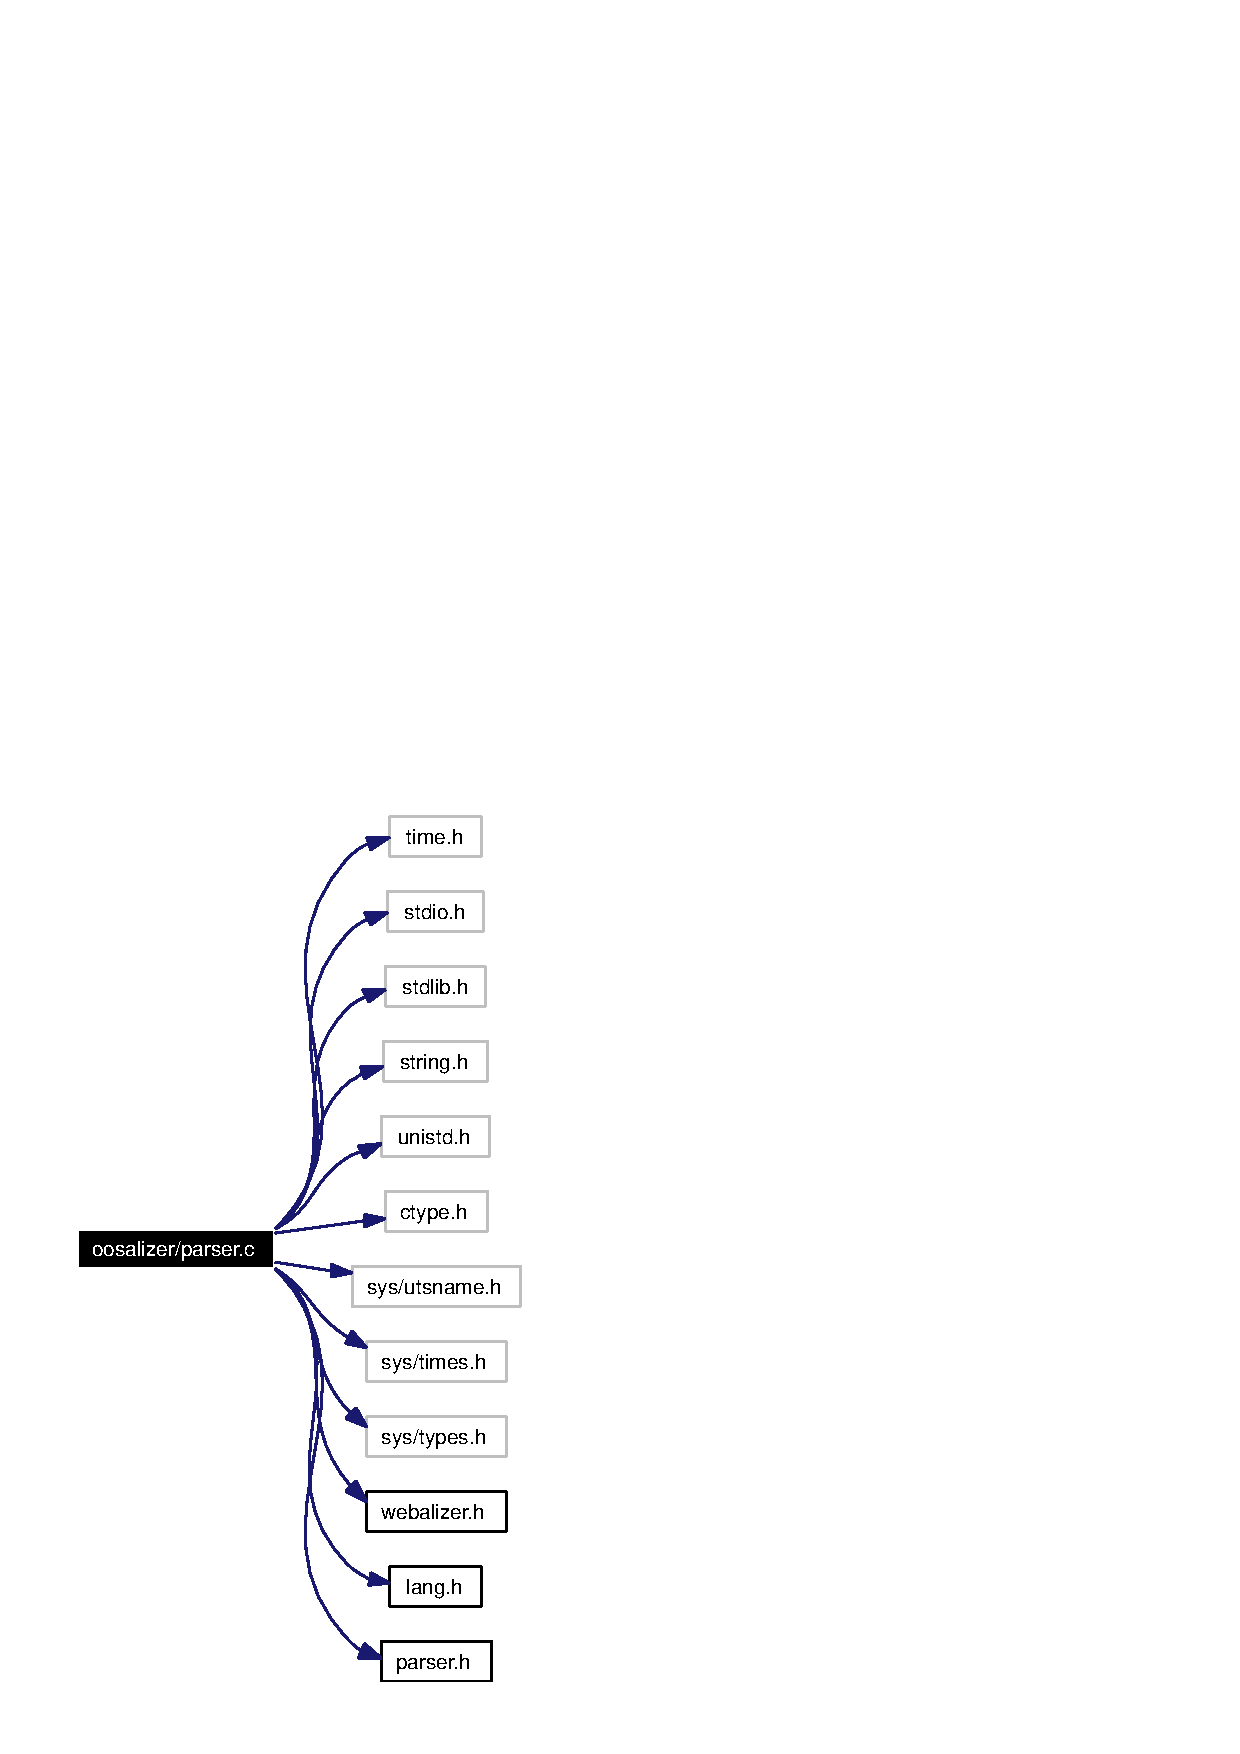
\includegraphics[width=125pt]{parser_8c__incl}
\end{center}
\end{figure}
\subsection*{Makrodefinitionen}
\begin{CompactItemize}
\item 
\#define {\bf CLK\_\-TCK}~\_\-SC\_\-CLK\_\-TCK
\end{CompactItemize}
\subsection*{Funktionen}
\begin{CompactItemize}
\item 
void {\bf fmt\_\-logrec} (char $\ast$)
\item 
int {\bf parse\_\-record\_\-web} (char $\ast$)
\item 
int {\bf parse\_\-record\_\-ftp} (char $\ast$)
\item 
int {\bf parse\_\-record\_\-squid} (char $\ast$)
\item 
int {\bf parse\_\-record} (char $\ast${\bf buffer})
\end{CompactItemize}


\subsection{Makro-Dokumentation}
\index{parser.c@{parser.c}!CLK_TCK@{CLK\_\-TCK}}
\index{CLK_TCK@{CLK\_\-TCK}!parser.c@{parser.c}}
\subsubsection{\setlength{\rightskip}{0pt plus 5cm}\#define CLK\_\-TCK~\_\-SC\_\-CLK\_\-TCK}\label{parser_8c_03df76d1f70664d745ca8de2864e39b3}




Definiert in Zeile 59 der Datei parser.c.

\subsection{Dokumentation der Funktionen}
\index{parser.c@{parser.c}!fmt_logrec@{fmt\_\-logrec}}
\index{fmt_logrec@{fmt\_\-logrec}!parser.c@{parser.c}}
\subsubsection{\setlength{\rightskip}{0pt plus 5cm}void fmt\_\-logrec (char $\ast$)}\label{parser_8c_05c2b956fa80dba2cd2fcce536158855}




Definiert in Zeile 76 der Datei parser.c.

Wird benutzt von parse\_\-record\_\-ftp(), parse\_\-record\_\-squid() und parse\_\-record\_\-web().\index{parser.c@{parser.c}!parse_record@{parse\_\-record}}
\index{parse_record@{parse\_\-record}!parser.c@{parser.c}}
\subsubsection{\setlength{\rightskip}{0pt plus 5cm}int parse\_\-record (char $\ast$ {\em buffer})}\label{parser_8c_f7f838e64a0d2b296d0b8b09b49d6b85}




Definiert in Zeile 101 der Datei parser.c.

Benutzt LOG\_\-CLF, LOG\_\-FTP, log\_\-rec, LOG\_\-SQUID, log\_\-type, parse\_\-record\_\-ftp(), parse\_\-record\_\-squid() und parse\_\-record\_\-web().\index{parser.c@{parser.c}!parse_record_ftp@{parse\_\-record\_\-ftp}}
\index{parse_record_ftp@{parse\_\-record\_\-ftp}!parser.c@{parser.c}}
\subsubsection{\setlength{\rightskip}{0pt plus 5cm}int parse\_\-record\_\-ftp (char $\ast$)}\label{parser_8c_630c3ac0dab48c2fba68649da4bb871e}




Definiert in Zeile 134 der Datei parser.c.

Benutzt log\_\-struct::datetime, fmt\_\-logrec(), log\_\-struct::hostname, log\_\-struct::ident, log\_\-rec, MAXHOST, MAXURL, log\_\-struct::resp\_\-code, log\_\-struct::url und log\_\-struct::xfer\_\-size.

Wird benutzt von parse\_\-record().\index{parser.c@{parser.c}!parse_record_squid@{parse\_\-record\_\-squid}}
\index{parse_record_squid@{parse\_\-record\_\-squid}!parser.c@{parser.c}}
\subsubsection{\setlength{\rightskip}{0pt plus 5cm}int parse\_\-record\_\-squid (char $\ast$)}\label{parser_8c_2b00ce99cc8f1387d75aeb7193968b21}




Definiert in Zeile 379 der Datei parser.c.

Benutzt log\_\-struct::datetime, debug\_\-mode, fmt\_\-logrec(), log\_\-struct::hostname, log\_\-struct::ident, log\_\-rec, MAXHOST, MAXIDENT, MAXURL, msg\_\-big\_\-host, msg\_\-big\_\-req, log\_\-struct::resp\_\-code, log\_\-struct::url, verbose und log\_\-struct::xfer\_\-size.

Wird benutzt von parse\_\-record().\index{parser.c@{parser.c}!parse_record_web@{parse\_\-record\_\-web}}
\index{parse_record_web@{parse\_\-record\_\-web}!parser.c@{parser.c}}
\subsubsection{\setlength{\rightskip}{0pt plus 5cm}int parse\_\-record\_\-web (char $\ast$)}\label{parser_8c_f79ff394bf86e83cffbcb560096f5052}




Definiert in Zeile 220 der Datei parser.c.

Benutzt log\_\-struct::agent, log\_\-struct::datetime, debug\_\-mode, fmt\_\-logrec(), log\_\-struct::hostname, log\_\-struct::ident, log\_\-rec, MAXAGENT, MAXHOST, MAXIDENT, MAXREF, MAXURL, msg\_\-big\_\-date, msg\_\-big\_\-host, msg\_\-big\_\-ref, msg\_\-big\_\-req, msg\_\-big\_\-user, log\_\-struct::refer, log\_\-struct::resp\_\-code, log\_\-struct::url, verbose und log\_\-struct::xfer\_\-size.

Wird benutzt von parse\_\-record().
\section{oosalizer/parser.h-Dateireferenz}
\label{parser_8h}\index{oosalizer/parser.h@{oosalizer/parser.h}}


Dieser Graph zeigt, welche Datei direkt oder indirekt diese Datei enth\"{a}lt:\begin{figure}[H]
\begin{center}
\leavevmode
\includegraphics[width=139pt]{parser_8h__dep__incl}
\end{center}
\end{figure}
\subsection*{Funktionen}
\begin{CompactItemize}
\item 
int {\bf parse\_\-record} (char $\ast$)
\end{CompactItemize}


\subsection{Dokumentation der Funktionen}
\index{parser.h@{parser.h}!parse_record@{parse\_\-record}}
\index{parse_record@{parse\_\-record}!parser.h@{parser.h}}
\subsubsection{\setlength{\rightskip}{0pt plus 5cm}int parse\_\-record (char $\ast$)}\label{parser_8h_2e298d5e806fc4936bf6b142c0913a31}




Definiert in Zeile 101 der Datei parser.c.

Benutzt LOG\_\-CLF, LOG\_\-FTP, log\_\-rec, LOG\_\-SQUID, log\_\-type, parse\_\-record\_\-ftp(), parse\_\-record\_\-squid() und parse\_\-record\_\-web().
\section{oosalizer/preserve.c-Dateireferenz}
\label{preserve_8c}\index{oosalizer/preserve.c@{oosalizer/preserve.c}}
{\tt \#include $<$time.h$>$}\par
{\tt \#include $<$stdio.h$>$}\par
{\tt \#include $<$stdlib.h$>$}\par
{\tt \#include $<$string.h$>$}\par
{\tt \#include $<$unistd.h$>$}\par
{\tt \#include $<$ctype.h$>$}\par
{\tt \#include $<$sys/utsname.h$>$}\par
{\tt \#include $<$sys/times.h$>$}\par
{\tt \#include $<$sys/types.h$>$}\par
{\tt \#include \char`\"{}webalizer.h\char`\"{}}\par
{\tt \#include \char`\"{}lang.h\char`\"{}}\par
{\tt \#include \char`\"{}hashtab.h\char`\"{}}\par
{\tt \#include \char`\"{}parser.h\char`\"{}}\par
{\tt \#include \char`\"{}preserve.h\char`\"{}}\par


Include-Abh\"{a}ngigkeitsdiagramm f\"{u}r preserve.c:\begin{figure}[H]
\begin{center}
\leavevmode
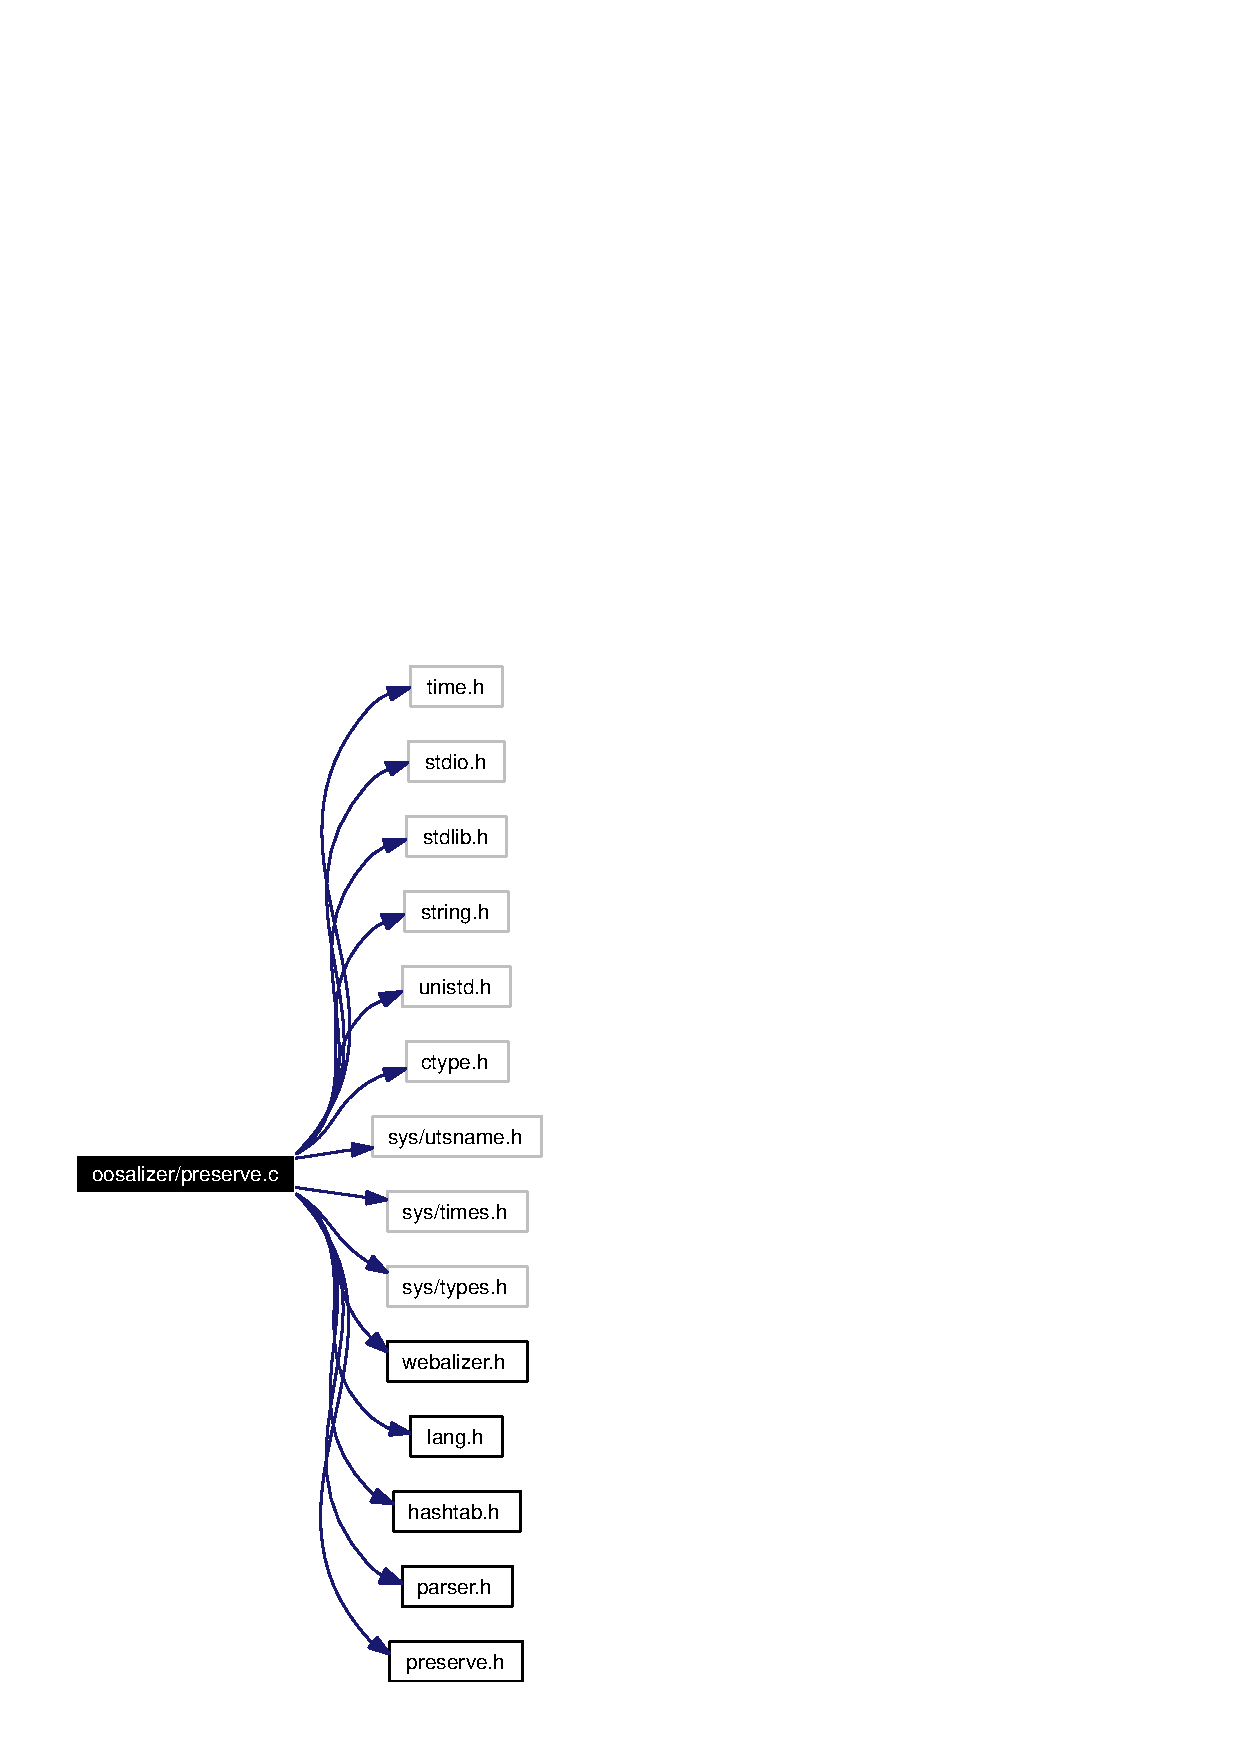
\includegraphics[width=130pt]{preserve_8c__incl}
\end{center}
\end{figure}
\subsection*{Makrodefinitionen}
\begin{CompactItemize}
\item 
\#define {\bf CLK\_\-TCK}~\_\-SC\_\-CLK\_\-TCK
\end{CompactItemize}
\subsection*{Funktionen}
\begin{CompactItemize}
\item 
void {\bf get\_\-history} ()
\item 
void {\bf put\_\-history} ()
\item 
int {\bf save\_\-state} ()
\item 
int {\bf restore\_\-state} ()
\end{CompactItemize}
\subsection*{Variablen}
\begin{CompactItemize}
\item 
int {\bf hist\_\-month} [12]
\item 
int {\bf hist\_\-year} [12]
\item 
u\_\-long {\bf hist\_\-hit} [12]
\item 
u\_\-long {\bf hist\_\-files} [12]
\item 
u\_\-long {\bf hist\_\-site} [12]
\item 
double {\bf hist\_\-xfer} [12]
\item 
u\_\-long {\bf hist\_\-page} [12]
\item 
u\_\-long {\bf hist\_\-visit} [12]
\item 
int {\bf hist\_\-fday} [12]
\item 
int {\bf hist\_\-lday} [12]
\end{CompactItemize}


\subsection{Makro-Dokumentation}
\index{preserve.c@{preserve.c}!CLK_TCK@{CLK\_\-TCK}}
\index{CLK_TCK@{CLK\_\-TCK}!preserve.c@{preserve.c}}
\subsubsection{\setlength{\rightskip}{0pt plus 5cm}\#define CLK\_\-TCK~\_\-SC\_\-CLK\_\-TCK}\label{preserve_8c_03df76d1f70664d745ca8de2864e39b3}




Definiert in Zeile 59 der Datei preserve.c.

\subsection{Dokumentation der Funktionen}
\index{preserve.c@{preserve.c}!get_history@{get\_\-history}}
\index{get_history@{get\_\-history}!preserve.c@{preserve.c}}
\subsubsection{\setlength{\rightskip}{0pt plus 5cm}void get\_\-history ()}\label{preserve_8c_d7ce84df67f8fe6fb2ae68f70445e3ff}




Definiert in Zeile 83 der Datei preserve.c.

Benutzt buffer, BUFSIZE, hist\_\-fday, hist\_\-files, hist\_\-hit, hist\_\-lday, hist\_\-month, hist\_\-page, hist\_\-site, hist\_\-visit, hist\_\-xfer und hist\_\-year.\index{preserve.c@{preserve.c}!put_history@{put\_\-history}}
\index{put_history@{put\_\-history}!preserve.c@{preserve.c}}
\subsubsection{\setlength{\rightskip}{0pt plus 5cm}void put\_\-history ()}\label{preserve_8c_0725425e14f501da1e2fc612d7854c01}




Definiert in Zeile 140 der Datei preserve.c.

Benutzt hist\_\-fday, hist\_\-files, hist\_\-fname, hist\_\-hit, hist\_\-lday, hist\_\-month, hist\_\-page, hist\_\-site, hist\_\-visit, hist\_\-xfer, hist\_\-year, msg\_\-put\_\-hist und verbose.\index{preserve.c@{preserve.c}!restore_state@{restore\_\-state}}
\index{restore_state@{restore\_\-state}!preserve.c@{preserve.c}}
\subsubsection{\setlength{\rightskip}{0pt plus 5cm}int restore\_\-state ()}\label{preserve_8c_87684b62a3f6bfdc76f25d5fb679c901}




Definiert in Zeile 405 der Datei preserve.c.

Benutzt BUFSIZE, cur\_\-day, cur\_\-hour, cur\_\-min, cur\_\-month, cur\_\-sec, cur\_\-tstamp, cur\_\-year, epoch, jdate(), msg\_\-get\_\-data, msg\_\-no\_\-data, state\_\-fname, t\_\-agent, t\_\-file, t\_\-hit, t\_\-page, t\_\-ref, t\_\-site, t\_\-url, t\_\-user, t\_\-visit, t\_\-xfer, tmp\_\-buf, ul\_\-bogus, verbose und version.\index{preserve.c@{preserve.c}!save_state@{save\_\-state}}
\index{save_state@{save\_\-state}!preserve.c@{preserve.c}}
\subsubsection{\setlength{\rightskip}{0pt plus 5cm}int save\_\-state ()}\label{preserve_8c_30d384683c4584a041792cf314051fa3}




Definiert in Zeile 178 der Datei preserve.c.

Benutzt buffer, BUFSIZE, cur\_\-day, cur\_\-hour, cur\_\-min, cur\_\-month, cur\_\-sec, cur\_\-year, dt\_\-site, editlvl, f\_\-day, ht\_\-hit, l\_\-day, mh\_\-hit, msg\_\-put\_\-data, state\_\-fname, t\_\-agent, t\_\-file, t\_\-hit, t\_\-page, t\_\-ref, t\_\-site, t\_\-url, t\_\-user, t\_\-visit, t\_\-xfer, tm\_\-file, tm\_\-hit, tm\_\-page, tm\_\-site, tm\_\-visit, tm\_\-xfer, verbose und version.

\subsection{Variablen-Dokumentation}
\index{preserve.c@{preserve.c}!hist_fday@{hist\_\-fday}}
\index{hist_fday@{hist\_\-fday}!preserve.c@{preserve.c}}
\subsubsection{\setlength{\rightskip}{0pt plus 5cm}int {\bf hist\_\-fday}[12]}\label{preserve_8c_aa2fe5b00c099187be9c1aace6552a9c}




Definiert in Zeile 77 der Datei preserve.c.

Wird benutzt von get\_\-history(), put\_\-history() und write\_\-month\_\-html().\index{preserve.c@{preserve.c}!hist_files@{hist\_\-files}}
\index{hist_files@{hist\_\-files}!preserve.c@{preserve.c}}
\subsubsection{\setlength{\rightskip}{0pt plus 5cm}u\_\-long {\bf hist\_\-files}[12]}\label{preserve_8c_5fce0b39aa3228d6b471e9294f1fed9d}




Definiert in Zeile 71 der Datei preserve.c.

Wird benutzt von get\_\-history(), put\_\-history() und write\_\-month\_\-html().\index{preserve.c@{preserve.c}!hist_hit@{hist\_\-hit}}
\index{hist_hit@{hist\_\-hit}!preserve.c@{preserve.c}}
\subsubsection{\setlength{\rightskip}{0pt plus 5cm}u\_\-long {\bf hist\_\-hit}[12]}\label{preserve_8c_71b324074ec02105c3730f77c0ab3e50}




Definiert in Zeile 70 der Datei preserve.c.

Wird benutzt von get\_\-history(), put\_\-history() und write\_\-month\_\-html().\index{preserve.c@{preserve.c}!hist_lday@{hist\_\-lday}}
\index{hist_lday@{hist\_\-lday}!preserve.c@{preserve.c}}
\subsubsection{\setlength{\rightskip}{0pt plus 5cm}int {\bf hist\_\-lday}[12]}\label{preserve_8c_c1366de31d95191e4f8fe0894dabb4e2}




Definiert in Zeile 77 der Datei preserve.c.

Wird benutzt von daily\_\-total\_\-table(), get\_\-history(), put\_\-history() und write\_\-month\_\-html().\index{preserve.c@{preserve.c}!hist_month@{hist\_\-month}}
\index{hist_month@{hist\_\-month}!preserve.c@{preserve.c}}
\subsubsection{\setlength{\rightskip}{0pt plus 5cm}int {\bf hist\_\-month}[12]}\label{preserve_8c_8dbdfde33bef98c2e3a8d2b8fab9143d}




Definiert in Zeile 69 der Datei preserve.c.

Wird benutzt von get\_\-history(), put\_\-history(), write\_\-main\_\-index() und write\_\-month\_\-html().\index{preserve.c@{preserve.c}!hist_page@{hist\_\-page}}
\index{hist_page@{hist\_\-page}!preserve.c@{preserve.c}}
\subsubsection{\setlength{\rightskip}{0pt plus 5cm}u\_\-long {\bf hist\_\-page}[12]}\label{preserve_8c_6885f98057e49be4b1a58cc1fea67b11}




Definiert in Zeile 74 der Datei preserve.c.

Wird benutzt von get\_\-history(), put\_\-history() und write\_\-month\_\-html().\index{preserve.c@{preserve.c}!hist_site@{hist\_\-site}}
\index{hist_site@{hist\_\-site}!preserve.c@{preserve.c}}
\subsubsection{\setlength{\rightskip}{0pt plus 5cm}u\_\-long {\bf hist\_\-site}[12]}\label{preserve_8c_95f554bfcd0bb37a1e90b29db92d2ffa}




Definiert in Zeile 72 der Datei preserve.c.

Wird benutzt von get\_\-history(), put\_\-history() und write\_\-month\_\-html().\index{preserve.c@{preserve.c}!hist_visit@{hist\_\-visit}}
\index{hist_visit@{hist\_\-visit}!preserve.c@{preserve.c}}
\subsubsection{\setlength{\rightskip}{0pt plus 5cm}u\_\-long {\bf hist\_\-visit}[12]}\label{preserve_8c_686df2d8a29e5dc08eddd9679fecc5ff}




Definiert in Zeile 75 der Datei preserve.c.

Wird benutzt von get\_\-history(), put\_\-history() und write\_\-month\_\-html().\index{preserve.c@{preserve.c}!hist_xfer@{hist\_\-xfer}}
\index{hist_xfer@{hist\_\-xfer}!preserve.c@{preserve.c}}
\subsubsection{\setlength{\rightskip}{0pt plus 5cm}double {\bf hist\_\-xfer}[12]}\label{preserve_8c_9258e499d6896ed681dbe7582d7047c4}




Definiert in Zeile 73 der Datei preserve.c.

Wird benutzt von get\_\-history(), put\_\-history() und write\_\-month\_\-html().\index{preserve.c@{preserve.c}!hist_year@{hist\_\-year}}
\index{hist_year@{hist\_\-year}!preserve.c@{preserve.c}}
\subsubsection{\setlength{\rightskip}{0pt plus 5cm}int {\bf hist\_\-year}[12]}\label{preserve_8c_bd6905416f4fb7c9cc62053f1f952d32}




Definiert in Zeile 69 der Datei preserve.c.

Wird benutzt von get\_\-history(), put\_\-history(), write\_\-main\_\-index() und write\_\-month\_\-html().
\section{oosalizer/preserve.h-Dateireferenz}
\label{preserve_8h}\index{oosalizer/preserve.h@{oosalizer/preserve.h}}


Dieser Graph zeigt, welche Datei direkt oder indirekt diese Datei enth\"{a}lt:\begin{figure}[H]
\begin{center}
\leavevmode
\includegraphics[width=145pt]{preserve_8h__dep__incl}
\end{center}
\end{figure}
\subsection*{Funktionen}
\begin{CompactItemize}
\item 
void {\bf get\_\-history} ()
\item 
void {\bf put\_\-history} ()
\item 
int {\bf save\_\-state} ()
\item 
int {\bf restore\_\-state} ()
\end{CompactItemize}
\subsection*{Variablen}
\begin{CompactItemize}
\item 
int {\bf hist\_\-month} [12]
\item 
int {\bf hist\_\-year} [12]
\item 
u\_\-long {\bf hist\_\-hit} [12]
\item 
u\_\-long {\bf hist\_\-files} [12]
\item 
u\_\-long {\bf hist\_\-site} [12]
\item 
double {\bf hist\_\-xfer} [12]
\item 
u\_\-long {\bf hist\_\-page} [12]
\item 
u\_\-long {\bf hist\_\-visit} [12]
\item 
int {\bf hist\_\-fday} [12]
\item 
int {\bf hist\_\-lday} [12]
\end{CompactItemize}


\subsection{Dokumentation der Funktionen}
\index{preserve.h@{preserve.h}!get_history@{get\_\-history}}
\index{get_history@{get\_\-history}!preserve.h@{preserve.h}}
\subsubsection{\setlength{\rightskip}{0pt plus 5cm}void get\_\-history ()}\label{preserve_8h_d7ce84df67f8fe6fb2ae68f70445e3ff}




Definiert in Zeile 83 der Datei preserve.c.

Benutzt buffer, BUFSIZE, hist\_\-fday, hist\_\-files, hist\_\-hit, hist\_\-lday, hist\_\-month, hist\_\-page, hist\_\-site, hist\_\-visit, hist\_\-xfer und hist\_\-year.\index{preserve.h@{preserve.h}!put_history@{put\_\-history}}
\index{put_history@{put\_\-history}!preserve.h@{preserve.h}}
\subsubsection{\setlength{\rightskip}{0pt plus 5cm}void put\_\-history ()}\label{preserve_8h_0725425e14f501da1e2fc612d7854c01}




Definiert in Zeile 140 der Datei preserve.c.

Benutzt hist\_\-fday, hist\_\-files, hist\_\-fname, hist\_\-hit, hist\_\-lday, hist\_\-month, hist\_\-page, hist\_\-site, hist\_\-visit, hist\_\-xfer, hist\_\-year, msg\_\-put\_\-hist und verbose.\index{preserve.h@{preserve.h}!restore_state@{restore\_\-state}}
\index{restore_state@{restore\_\-state}!preserve.h@{preserve.h}}
\subsubsection{\setlength{\rightskip}{0pt plus 5cm}int restore\_\-state ()}\label{preserve_8h_87684b62a3f6bfdc76f25d5fb679c901}




Definiert in Zeile 405 der Datei preserve.c.

Benutzt BUFSIZE, cur\_\-day, cur\_\-hour, cur\_\-min, cur\_\-month, cur\_\-sec, cur\_\-tstamp, cur\_\-year, epoch, jdate(), msg\_\-get\_\-data, msg\_\-no\_\-data, state\_\-fname, t\_\-agent, t\_\-file, t\_\-hit, t\_\-page, t\_\-ref, t\_\-site, t\_\-url, t\_\-user, t\_\-visit, t\_\-xfer, tmp\_\-buf, ul\_\-bogus, verbose und version.\index{preserve.h@{preserve.h}!save_state@{save\_\-state}}
\index{save_state@{save\_\-state}!preserve.h@{preserve.h}}
\subsubsection{\setlength{\rightskip}{0pt plus 5cm}int save\_\-state ()}\label{preserve_8h_30d384683c4584a041792cf314051fa3}




Definiert in Zeile 178 der Datei preserve.c.

Benutzt buffer, BUFSIZE, cur\_\-day, cur\_\-hour, cur\_\-min, cur\_\-month, cur\_\-sec, cur\_\-year, dt\_\-site, editlvl, f\_\-day, ht\_\-hit, l\_\-day, mh\_\-hit, msg\_\-put\_\-data, state\_\-fname, t\_\-agent, t\_\-file, t\_\-hit, t\_\-page, t\_\-ref, t\_\-site, t\_\-url, t\_\-user, t\_\-visit, t\_\-xfer, tm\_\-file, tm\_\-hit, tm\_\-page, tm\_\-site, tm\_\-visit, tm\_\-xfer, verbose und version.

\subsection{Variablen-Dokumentation}
\index{preserve.h@{preserve.h}!hist_fday@{hist\_\-fday}}
\index{hist_fday@{hist\_\-fday}!preserve.h@{preserve.h}}
\subsubsection{\setlength{\rightskip}{0pt plus 5cm}int {\bf hist\_\-fday}[12]}\label{preserve_8h_aa2fe5b00c099187be9c1aace6552a9c}




Definiert in Zeile 77 der Datei preserve.c.

Wird benutzt von get\_\-history(), put\_\-history() und write\_\-month\_\-html().\index{preserve.h@{preserve.h}!hist_files@{hist\_\-files}}
\index{hist_files@{hist\_\-files}!preserve.h@{preserve.h}}
\subsubsection{\setlength{\rightskip}{0pt plus 5cm}u\_\-long {\bf hist\_\-files}[12]}\label{preserve_8h_5fce0b39aa3228d6b471e9294f1fed9d}




Definiert in Zeile 71 der Datei preserve.c.

Wird benutzt von get\_\-history(), put\_\-history() und write\_\-month\_\-html().\index{preserve.h@{preserve.h}!hist_hit@{hist\_\-hit}}
\index{hist_hit@{hist\_\-hit}!preserve.h@{preserve.h}}
\subsubsection{\setlength{\rightskip}{0pt plus 5cm}u\_\-long {\bf hist\_\-hit}[12]}\label{preserve_8h_71b324074ec02105c3730f77c0ab3e50}




Definiert in Zeile 70 der Datei preserve.c.

Wird benutzt von get\_\-history(), put\_\-history() und write\_\-month\_\-html().\index{preserve.h@{preserve.h}!hist_lday@{hist\_\-lday}}
\index{hist_lday@{hist\_\-lday}!preserve.h@{preserve.h}}
\subsubsection{\setlength{\rightskip}{0pt plus 5cm}int {\bf hist\_\-lday}[12]}\label{preserve_8h_c1366de31d95191e4f8fe0894dabb4e2}




Definiert in Zeile 77 der Datei preserve.c.

Wird benutzt von daily\_\-total\_\-table(), get\_\-history(), put\_\-history() und write\_\-month\_\-html().\index{preserve.h@{preserve.h}!hist_month@{hist\_\-month}}
\index{hist_month@{hist\_\-month}!preserve.h@{preserve.h}}
\subsubsection{\setlength{\rightskip}{0pt plus 5cm}int {\bf hist\_\-month}[12]}\label{preserve_8h_8dbdfde33bef98c2e3a8d2b8fab9143d}




Definiert in Zeile 69 der Datei preserve.c.

Wird benutzt von get\_\-history(), put\_\-history(), write\_\-main\_\-index() und write\_\-month\_\-html().\index{preserve.h@{preserve.h}!hist_page@{hist\_\-page}}
\index{hist_page@{hist\_\-page}!preserve.h@{preserve.h}}
\subsubsection{\setlength{\rightskip}{0pt plus 5cm}u\_\-long {\bf hist\_\-page}[12]}\label{preserve_8h_6885f98057e49be4b1a58cc1fea67b11}




Definiert in Zeile 74 der Datei preserve.c.

Wird benutzt von get\_\-history(), put\_\-history() und write\_\-month\_\-html().\index{preserve.h@{preserve.h}!hist_site@{hist\_\-site}}
\index{hist_site@{hist\_\-site}!preserve.h@{preserve.h}}
\subsubsection{\setlength{\rightskip}{0pt plus 5cm}u\_\-long {\bf hist\_\-site}[12]}\label{preserve_8h_95f554bfcd0bb37a1e90b29db92d2ffa}




Definiert in Zeile 72 der Datei preserve.c.

Wird benutzt von get\_\-history(), put\_\-history() und write\_\-month\_\-html().\index{preserve.h@{preserve.h}!hist_visit@{hist\_\-visit}}
\index{hist_visit@{hist\_\-visit}!preserve.h@{preserve.h}}
\subsubsection{\setlength{\rightskip}{0pt plus 5cm}u\_\-long {\bf hist\_\-visit}[12]}\label{preserve_8h_686df2d8a29e5dc08eddd9679fecc5ff}




Definiert in Zeile 75 der Datei preserve.c.

Wird benutzt von get\_\-history(), put\_\-history() und write\_\-month\_\-html().\index{preserve.h@{preserve.h}!hist_xfer@{hist\_\-xfer}}
\index{hist_xfer@{hist\_\-xfer}!preserve.h@{preserve.h}}
\subsubsection{\setlength{\rightskip}{0pt plus 5cm}double {\bf hist\_\-xfer}[12]}\label{preserve_8h_9258e499d6896ed681dbe7582d7047c4}




Definiert in Zeile 73 der Datei preserve.c.

Wird benutzt von get\_\-history(), put\_\-history() und write\_\-month\_\-html().\index{preserve.h@{preserve.h}!hist_year@{hist\_\-year}}
\index{hist_year@{hist\_\-year}!preserve.h@{preserve.h}}
\subsubsection{\setlength{\rightskip}{0pt plus 5cm}int {\bf hist\_\-year}[12]}\label{preserve_8h_bd6905416f4fb7c9cc62053f1f952d32}




Definiert in Zeile 69 der Datei preserve.c.

Wird benutzt von get\_\-history(), put\_\-history(), write\_\-main\_\-index() und write\_\-month\_\-html().
\section{oosalizer/webalizer.c-Dateireferenz}
\label{webalizer_8c}\index{oosalizer/webalizer.c@{oosalizer/webalizer.c}}
{\tt \#include $<$time.h$>$}\par
{\tt \#include $<$stdio.h$>$}\par
{\tt \#include $<$stdlib.h$>$}\par
{\tt \#include $<$string.h$>$}\par
{\tt \#include $<$unistd.h$>$}\par
{\tt \#include $<$ctype.h$>$}\par
{\tt \#include $<$sys/utsname.h$>$}\par
{\tt \#include $<$sys/times.h$>$}\par
{\tt \#include $<$zlib.h$>$}\par
{\tt \#include $<$sys/types.h$>$}\par
{\tt \#include \char`\"{}webalizer.h\char`\"{}}\par
{\tt \#include \char`\"{}output.h\char`\"{}}\par
{\tt \#include \char`\"{}parser.h\char`\"{}}\par
{\tt \#include \char`\"{}preserve.h\char`\"{}}\par
{\tt \#include \char`\"{}hashtab.h\char`\"{}}\par
{\tt \#include \char`\"{}linklist.h\char`\"{}}\par
{\tt \#include \char`\"{}webalizer\_\-lang.h\char`\"{}}\par


Include-Abh\"{a}ngigkeitsdiagramm f\"{u}r webalizer.c:\begin{figure}[H]
\begin{center}
\leavevmode
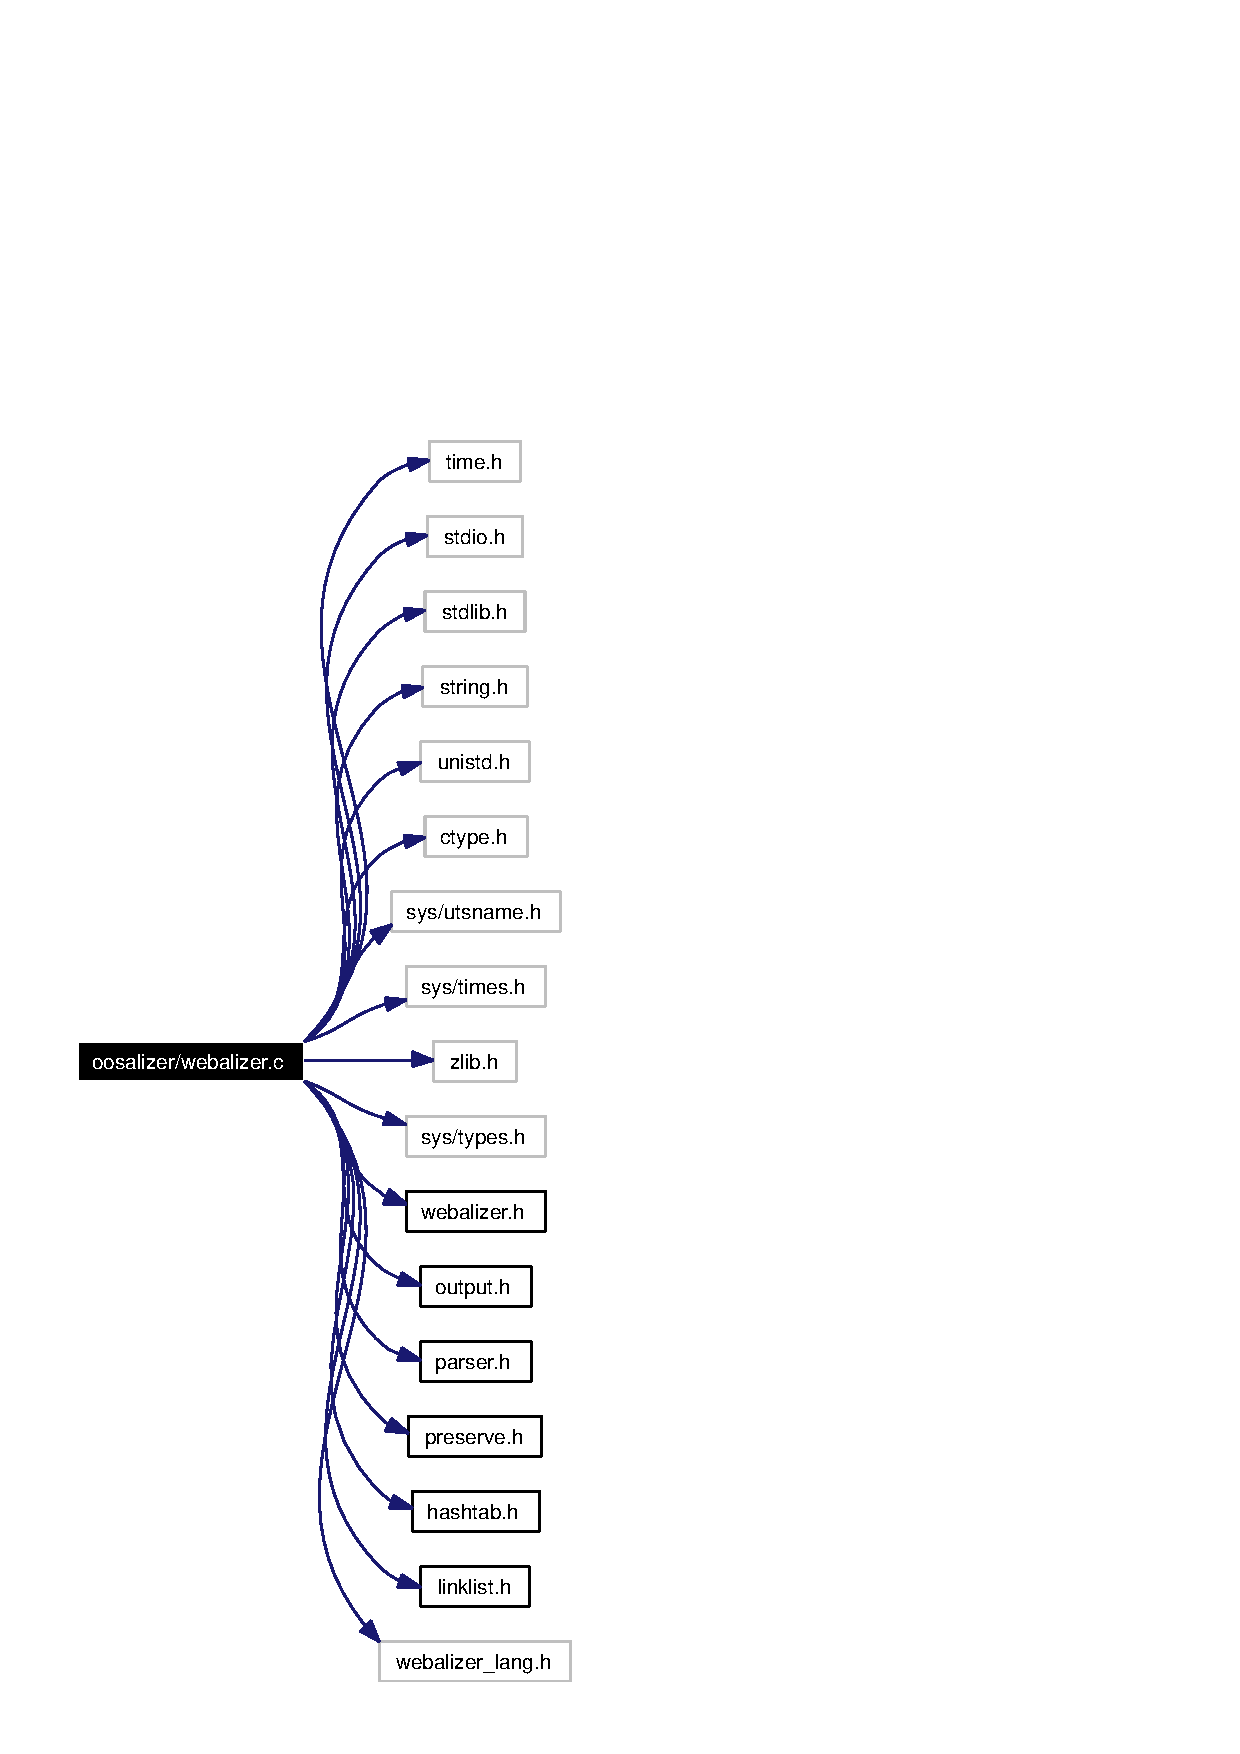
\includegraphics[width=137pt]{webalizer_8c__incl}
\end{center}
\end{figure}
\subsection*{Makrodefinitionen}
\begin{CompactItemize}
\item 
\#define {\bf CLK\_\-TCK}~\_\-SC\_\-CLK\_\-TCK
\item 
\#define {\bf GZ\_\-BUFSIZE}~16384
\end{CompactItemize}
\subsection*{Funktionen}
\begin{CompactItemize}
\item 
void {\bf clear\_\-month} ()
\item 
char $\ast$ {\bf unescape} (char $\ast$)
\item 
char {\bf from\_\-hex} (char)
\item 
void {\bf print\_\-opts} (char $\ast$)
\item 
void {\bf print\_\-version} ()
\item 
int {\bf isurlchar} (unsigned char)
\item 
void {\bf get\_\-config} (char $\ast$)
\item 
static char $\ast$ {\bf save\_\-opt} (char $\ast$)
\item 
void {\bf srch\_\-string} (char $\ast$)
\item 
char $\ast$ {\bf get\_\-domain} (char $\ast$)
\item 
char $\ast$ {\bf our\_\-gzgets} (gz\-File, char $\ast$, int)
\item 
int {\bf main} (int argc, char $\ast$argv[$\,$])
\item 
void {\bf init\_\-counters} ()
\item 
char $\ast$ {\bf cur\_\-time} ()
\item 
int {\bf ispage} (char $\ast$str)
\item 
u\_\-long {\bf ctry\_\-idx} (char $\ast$str)
\item 
u\_\-long {\bf jdate} (int day, int month, int year)
\end{CompactItemize}
\subsection*{Variablen}
\begin{CompactItemize}
\item 
char $\ast$ {\bf version} = \char`\"{}2.01\char`\"{}
\item 
char $\ast$ {\bf editlvl} = \char`\"{}10\char`\"{}
\item 
char $\ast$ {\bf moddate} = \char`\"{}16-Apr-2002\char`\"{}
\item 
char $\ast$ {\bf copyright} = \char`\"{}Copyright 1997-2001 by Bradford L. Barrett\char`\"{}
\item 
int {\bf verbose} = 2
\item 
int {\bf debug\_\-mode} = 0
\item 
int {\bf time\_\-me} = 0
\item 
int {\bf local\_\-time} = 1
\item 
int {\bf ignore\_\-hist} = 0
\item 
int {\bf hourly\_\-graph} = 1
\item 
int {\bf hourly\_\-stats} = 1
\item 
int {\bf daily\_\-graph} = 1
\item 
int {\bf daily\_\-stats} = 1
\item 
int {\bf ctry\_\-graph} = 1
\item 
int {\bf shade\_\-groups} = 1
\item 
int {\bf hlite\_\-groups} = 1
\item 
int {\bf mangle\_\-agent} = 0
\item 
int {\bf incremental} = 0
\item 
int {\bf use\_\-https} = 0
\item 
int {\bf visit\_\-timeout} = 1800
\item 
int {\bf graph\_\-legend} = 1
\item 
int {\bf graph\_\-lines} = 2
\item 
int {\bf fold\_\-seq\_\-err} = 0
\item 
int {\bf log\_\-type} = LOG\_\-CLF
\item 
int {\bf group\_\-domains} = 0
\item 
int {\bf hide\_\-sites} = 0
\item 
char $\ast$ {\bf hname} = NULL
\item 
char $\ast$ {\bf state\_\-fname} = \char`\"{}webalizer.current\char`\"{}
\item 
char $\ast$ {\bf hist\_\-fname} = \char`\"{}webalizer.hist\char`\"{}
\item 
char $\ast$ {\bf html\_\-ext} = \char`\"{}html\char`\"{}
\item 
char $\ast$ {\bf dump\_\-ext} = \char`\"{}tab\char`\"{}
\item 
char $\ast$ {\bf conf\_\-fname} = NULL
\item 
char $\ast$ {\bf log\_\-fname} = NULL
\item 
char $\ast$ {\bf out\_\-dir} = NULL
\item 
char $\ast$ {\bf blank\_\-str} = \char`\"{}\char`\"{}
\item 
char $\ast$ {\bf dns\_\-cache} = NULL
\item 
int {\bf dns\_\-children} = 0
\item 
int {\bf ntop\_\-sites} = 30
\item 
int {\bf ntop\_\-sites\-K} = 10
\item 
int {\bf ntop\_\-urls} = 30
\item 
int {\bf ntop\_\-urls\-K} = 10
\item 
int {\bf ntop\_\-entry} = 10
\item 
int {\bf ntop\_\-exit} = 10
\item 
int {\bf ntop\_\-refs} = 30
\item 
int {\bf ntop\_\-agents} = 15
\item 
int {\bf ntop\_\-ctrys} = 30
\item 
int {\bf ntop\_\-search} = 20
\item 
int {\bf ntop\_\-users} = 20
\item 
int {\bf ntop\_\-notfound} = 50
\item 
int {\bf all\_\-sites} = 0
\item 
int {\bf all\_\-urls} = 0
\item 
int {\bf all\_\-refs} = 0
\item 
int {\bf all\_\-agents} = 0
\item 
int {\bf all\_\-search} = 0
\item 
int {\bf all\_\-users} = 0
\item 
int {\bf dump\_\-sites} = 0
\item 
int {\bf dump\_\-urls} = 0
\item 
int {\bf dump\_\-refs} = 0
\item 
int {\bf dump\_\-agents} = 0
\item 
int {\bf dump\_\-users} = 0
\item 
int {\bf dump\_\-search} = 0
\item 
int {\bf dump\_\-header} = 0
\item 
char $\ast$ {\bf dump\_\-path} = NULL
\item 
int {\bf cur\_\-year} = 0
\item 
int {\bf cur\_\-month} = 0
\item 
int {\bf cur\_\-day} = 0
\item 
int {\bf cur\_\-hour} = 0
\item 
int {\bf cur\_\-min} = 0
\item 
int {\bf cur\_\-sec} = 0
\item 
u\_\-long {\bf cur\_\-tstamp} = 0
\item 
u\_\-long {\bf rec\_\-tstamp} = 0
\item 
u\_\-long {\bf req\_\-tstamp} = 0
\item 
u\_\-long {\bf epoch}
\item 
int {\bf check\_\-dup} = 0
\item 
int {\bf gz\_\-log} = 0
\item 
double {\bf t\_\-xfer} = 0.0
\item 
u\_\-long {\bf t\_\-hit} = 0
\item 
u\_\-long {\bf t\_\-file} = 0
\item 
u\_\-long {\bf t\_\-site} = 0
\item 
u\_\-long {\bf t\_\-url} = 0
\item 
u\_\-long {\bf t\_\-ref} = 0
\item 
u\_\-long {\bf t\_\-agent} = 0
\item 
u\_\-long {\bf t\_\-page} = 0
\item 
u\_\-long {\bf t\_\-visit} = 0
\item 
u\_\-long {\bf t\_\-user} = 0
\item 
double {\bf tm\_\-xfer} [31]
\item 
u\_\-long {\bf tm\_\-hit} [31]
\item 
u\_\-long {\bf tm\_\-file} [31]
\item 
u\_\-long {\bf tm\_\-site} [31]
\item 
u\_\-long {\bf tm\_\-page} [31]
\item 
u\_\-long {\bf tm\_\-visit} [31]
\item 
u\_\-long {\bf dt\_\-site}
\item 
u\_\-long {\bf ht\_\-hit} = 0
\item 
u\_\-long {\bf mh\_\-hit} = 0
\item 
u\_\-long {\bf th\_\-hit} [24]
\item 
u\_\-long {\bf th\_\-file} [24]
\item 
u\_\-long {\bf th\_\-page} [24]
\item 
double {\bf th\_\-xfer} [24]
\item 
int {\bf f\_\-day}
\item 
int {\bf l\_\-day}
\item 
utsname {\bf system\_\-info}
\item 
u\_\-long {\bf ul\_\-bogus} = 0
\item 
{\bf log\_\-struct} {\bf log\_\-rec}
\item 
time\_\-t {\bf now}
\item 
tm $\ast$ {\bf tp}
\item 
char {\bf timestamp} [32]
\item 
gz\-File {\bf gzlog\_\-fp}
\item 
FILE $\ast$ {\bf log\_\-fp}
\item 
char {\bf buffer} [BUFSIZE]
\item 
char {\bf tmp\_\-buf} [BUFSIZE]
\item 
{\bf CLISTPTR} $\ast$ {\bf top\_\-ctrys} = NULL
\item 
char {\bf f\_\-buf} [GZ\_\-BUFSIZE]
\item 
char $\ast$ {\bf f\_\-cp} = {\bf f\_\-buf}+GZ\_\-BUFSIZE
\item 
int {\bf f\_\-end}
\end{CompactItemize}


\subsection{Makro-Dokumentation}
\index{webalizer.c@{webalizer.c}!CLK_TCK@{CLK\_\-TCK}}
\index{CLK_TCK@{CLK\_\-TCK}!webalizer.c@{webalizer.c}}
\subsubsection{\setlength{\rightskip}{0pt plus 5cm}\#define CLK\_\-TCK~\_\-SC\_\-CLK\_\-TCK}\label{webalizer_8c_03df76d1f70664d745ca8de2864e39b3}




Definiert in Zeile 60 der Datei webalizer.c.\index{webalizer.c@{webalizer.c}!GZ_BUFSIZE@{GZ\_\-BUFSIZE}}
\index{GZ_BUFSIZE@{GZ\_\-BUFSIZE}!webalizer.c@{webalizer.c}}
\subsubsection{\setlength{\rightskip}{0pt plus 5cm}\#define GZ\_\-BUFSIZE~16384}\label{webalizer_8c_0ca8208fe0ebf85a7d26cb53c31f8a78}




Definiert in Zeile 223 der Datei webalizer.c.

Wird benutzt von our\_\-gzgets().

\subsection{Dokumentation der Funktionen}
\index{webalizer.c@{webalizer.c}!clear_month@{clear\_\-month}}
\index{clear_month@{clear\_\-month}!webalizer.c@{webalizer.c}}
\subsubsection{\setlength{\rightskip}{0pt plus 5cm}void clear\_\-month ()}\label{webalizer_8c_3d6b75394204fbb3dbe30423911cda44}




Definiert in Zeile 1701 der Datei webalizer.c.

Benutzt del\_\-htabs(), init\_\-counters(), ntop\_\-ctrys und top\_\-ctrys.\index{webalizer.c@{webalizer.c}!ctry_idx@{ctry\_\-idx}}
\index{ctry_idx@{ctry\_\-idx}!webalizer.c@{webalizer.c}}
\subsubsection{\setlength{\rightskip}{0pt plus 5cm}u\_\-long ctry\_\-idx (char $\ast$ {\em str})}\label{webalizer_8c_154bd0b4bda40aa5c99d7cf79886d400}




Definiert in Zeile 1827 der Datei webalizer.c.\index{webalizer.c@{webalizer.c}!cur_time@{cur\_\-time}}
\index{cur_time@{cur\_\-time}!webalizer.c@{webalizer.c}}
\subsubsection{\setlength{\rightskip}{0pt plus 5cm}char$\ast$ cur\_\-time ()}\label{webalizer_8c_f6fc05ecb3c962ea69fac0a9ce9525d7}




Definiert in Zeile 1783 der Datei webalizer.c.

Benutzt local\_\-time, now und timestamp.

Wird benutzt von write\_\-html\_\-head().\index{webalizer.c@{webalizer.c}!from_hex@{from\_\-hex}}
\index{from_hex@{from\_\-hex}!webalizer.c@{webalizer.c}}
\subsubsection{\setlength{\rightskip}{0pt plus 5cm}char from\_\-hex (char)}\label{webalizer_8c_9f2fa07c0c39a7caed8e40eaf1c2fa96}




Definiert in Zeile 1840 der Datei webalizer.c.

Wird benutzt von unescape().\index{webalizer.c@{webalizer.c}!get_config@{get\_\-config}}
\index{get_config@{get\_\-config}!webalizer.c@{webalizer.c}}
\subsubsection{\setlength{\rightskip}{0pt plus 5cm}void get\_\-config (char $\ast$)}\label{webalizer_8c_7e50c67e6aba9c0c3025c04b0a7aedc4}




Definiert in Zeile 1443 der Datei webalizer.c.

Benutzt BUFSIZE, msg\_\-bad\_\-conf, msg\_\-bad\_\-key und verbose.

Wird benutzt von main().\index{webalizer.c@{webalizer.c}!get_domain@{get\_\-domain}}
\index{get_domain@{get\_\-domain}!webalizer.c@{webalizer.c}}
\subsubsection{\setlength{\rightskip}{0pt plus 5cm}char $\ast$ get\_\-domain (char $\ast$)}\label{webalizer_8c_4c24c3d81b9c48e9f490919de3e32afb}




Definiert in Zeile 1942 der Datei webalizer.c.

Benutzt group\_\-domains.\index{webalizer.c@{webalizer.c}!init_counters@{init\_\-counters}}
\index{init_counters@{init\_\-counters}!webalizer.c@{webalizer.c}}
\subsubsection{\setlength{\rightskip}{0pt plus 5cm}void init\_\-counters ()}\label{webalizer_8c_c13990c5857877d516d60af22bfbc492}




Definiert in Zeile 1714 der Datei webalizer.c.

Benutzt response\_\-url::count, response, tm\_\-file, tm\_\-hit, tm\_\-page, tm\_\-site, tm\_\-visit, tm\_\-xfer und TOTAL\_\-RC.

Wird benutzt von clear\_\-month() und main().\index{webalizer.c@{webalizer.c}!ispage@{ispage}}
\index{ispage@{ispage}!webalizer.c@{webalizer.c}}
\subsubsection{\setlength{\rightskip}{0pt plus 5cm}int ispage (char $\ast$ {\em str})}\label{webalizer_8c_875f50fc519d72b2f46b8413cb1a9c45}




Definiert in Zeile 1802 der Datei webalizer.c.

Benutzt isinlist() und page\_\-type.

Wird benutzt von put\_\-hnode() und put\_\-inode().\index{webalizer.c@{webalizer.c}!isurlchar@{isurlchar}}
\index{isurlchar@{isurlchar}!webalizer.c@{webalizer.c}}
\subsubsection{\setlength{\rightskip}{0pt plus 5cm}int isurlchar (unsigned {\em char})}\label{webalizer_8c_6889c498251013344e6bcd437b077db0}




Definiert in Zeile 1816 der Datei webalizer.c.\index{webalizer.c@{webalizer.c}!jdate@{jdate}}
\index{jdate@{jdate}!webalizer.c@{webalizer.c}}
\subsubsection{\setlength{\rightskip}{0pt plus 5cm}u\_\-long jdate (int {\em day}, int {\em month}, int {\em year})}\label{webalizer_8c_8fb8978d91b70fd80d00d381cb115731}




Definiert in Zeile 2009 der Datei webalizer.c.

Wird benutzt von main(), month\_\-graph6() und restore\_\-state().\index{webalizer.c@{webalizer.c}!main@{main}}
\index{main@{main}!webalizer.c@{webalizer.c}}
\subsubsection{\setlength{\rightskip}{0pt plus 5cm}int main (int {\em argc}, char $\ast$ {\em argv}[$\,$])}\label{webalizer_8c_0ddf1224851353fc92bfbff6f499fa97}




Definiert in Zeile 232 der Datei webalizer.c.

Benutzt add\_\-nlist(), ctry, ctry\_\-graph, debug\_\-mode, country\_\-code::desc, dns\_\-cache, dns\_\-children, epoch, fold\_\-seq\_\-err, get\_\-config(), graph\_\-legend, graph\_\-lines, group\_\-domains, gz\_\-log, hidden\_\-agents, hidden\_\-refs, hidden\_\-sites, hidden\_\-urls, hide\_\-sites, hname, hourly\_\-graph, hourly\_\-stats, html\_\-ext, ignore\_\-hist, incremental, index\_\-alias, init\_\-counters(), isinlist(), jdate(), LOG\_\-CLF, log\_\-fname, LOG\_\-FTP, LOG\_\-SQUID, log\_\-type, mangle\_\-agent, MAXRESP, msg\_\-title, ntop\_\-agents, ntop\_\-ctrys, ntop\_\-entry, ntop\_\-exit, ntop\_\-refs, ntop\_\-search, ntop\_\-sites, ntop\_\-urls, out\_\-dir, page\_\-type, print\_\-opts(), print\_\-version(), resp\_\-counter, respnotfound, time\_\-me, tmp\_\-buf, verbose und visit\_\-timeout.\index{webalizer.c@{webalizer.c}!our_gzgets@{our\_\-gzgets}}
\index{our_gzgets@{our\_\-gzgets}!webalizer.c@{webalizer.c}}
\subsubsection{\setlength{\rightskip}{0pt plus 5cm}char $\ast$ our\_\-gzgets (gz\-File, char $\ast$, int)}\label{webalizer_8c_8abb48bca3dbb868295ee2ce344e3d95}




Definiert in Zeile 1963 der Datei webalizer.c.

Benutzt f\_\-buf, f\_\-cp, f\_\-end und GZ\_\-BUFSIZE.\index{webalizer.c@{webalizer.c}!print_opts@{print\_\-opts}}
\index{print_opts@{print\_\-opts}!webalizer.c@{webalizer.c}}
\subsubsection{\setlength{\rightskip}{0pt plus 5cm}void print\_\-opts (char $\ast$)}\label{webalizer_8c_beb1db8f30c512b9050440ec49248364}




Definiert in Zeile 1744 der Datei webalizer.c.

Benutzt h\_\-msg, h\_\-usage1 und h\_\-usage2.

Wird benutzt von main().\index{webalizer.c@{webalizer.c}!print_version@{print\_\-version}}
\index{print_version@{print\_\-version}!webalizer.c@{webalizer.c}}
\subsubsection{\setlength{\rightskip}{0pt plus 5cm}void print\_\-version ()}\label{webalizer_8c_6302aaae12249e8ea16bfdc7de892f21}




Definiert in Zeile 1757 der Datei webalizer.c.

Benutzt copyright, debug\_\-mode, editlvl, language, moddate, system\_\-info und version.

Wird benutzt von main().\index{webalizer.c@{webalizer.c}!save_opt@{save\_\-opt}}
\index{save_opt@{save\_\-opt}!webalizer.c@{webalizer.c}}
\subsubsection{\setlength{\rightskip}{0pt plus 5cm}static char $\ast$ save\_\-opt (char $\ast$)\hspace{0.3cm}{\tt  [static]}}\label{webalizer_8c_90af490e0665082d8b56fea2667356f4}




Definiert in Zeile 1687 der Datei webalizer.c.\index{webalizer.c@{webalizer.c}!srch_string@{srch\_\-string}}
\index{srch_string@{srch\_\-string}!webalizer.c@{webalizer.c}}
\subsubsection{\setlength{\rightskip}{0pt plus 5cm}void srch\_\-string (char $\ast$)}\label{webalizer_8c_2b1002ec17d1cd1e6901514b8b6de058}




Definiert in Zeile 1883 der Datei webalizer.c.

Benutzt BUFSIZE, isinglist(), log\_\-rec, msg\_\-nomem\_\-sc, put\_\-snode(), log\_\-struct::refer, search\_\-list, sr\_\-htab und verbose.\index{webalizer.c@{webalizer.c}!unescape@{unescape}}
\index{unescape@{unescape}!webalizer.c@{webalizer.c}}
\subsubsection{\setlength{\rightskip}{0pt plus 5cm}char $\ast$ unescape (char $\ast$)}\label{webalizer_8c_5d5d55b66d7df3272cf98f061b6fd2f6}




Definiert in Zeile 1852 der Datei webalizer.c.

Benutzt from\_\-hex().

\subsection{Variablen-Dokumentation}
\index{webalizer.c@{webalizer.c}!all_agents@{all\_\-agents}}
\index{all_agents@{all\_\-agents}!webalizer.c@{webalizer.c}}
\subsubsection{\setlength{\rightskip}{0pt plus 5cm}int {\bf all\_\-agents} = 0}\label{webalizer_8c_e6a5e084455a29d95c410b6e6f509c07}




Definiert in Zeile 158 der Datei webalizer.c.

Wird benutzt von top\_\-agents\_\-table().\index{webalizer.c@{webalizer.c}!all_refs@{all\_\-refs}}
\index{all_refs@{all\_\-refs}!webalizer.c@{webalizer.c}}
\subsubsection{\setlength{\rightskip}{0pt plus 5cm}int {\bf all\_\-refs} = 0}\label{webalizer_8c_5d9ecc711cb4edb47133e9c8329a2f6a}




Definiert in Zeile 157 der Datei webalizer.c.

Wird benutzt von top\_\-refs\_\-table().\index{webalizer.c@{webalizer.c}!all_search@{all\_\-search}}
\index{all_search@{all\_\-search}!webalizer.c@{webalizer.c}}
\subsubsection{\setlength{\rightskip}{0pt plus 5cm}int {\bf all\_\-search} = 0}\label{webalizer_8c_f51b93932a98e306bd47239ec9c99f23}




Definiert in Zeile 159 der Datei webalizer.c.

Wird benutzt von top\_\-search\_\-table().\index{webalizer.c@{webalizer.c}!all_sites@{all\_\-sites}}
\index{all_sites@{all\_\-sites}!webalizer.c@{webalizer.c}}
\subsubsection{\setlength{\rightskip}{0pt plus 5cm}int {\bf all\_\-sites} = 0}\label{webalizer_8c_e80c0d7d06836110749922f34dd902c2}




Definiert in Zeile 155 der Datei webalizer.c.

Wird benutzt von top\_\-sites\_\-table().\index{webalizer.c@{webalizer.c}!all_urls@{all\_\-urls}}
\index{all_urls@{all\_\-urls}!webalizer.c@{webalizer.c}}
\subsubsection{\setlength{\rightskip}{0pt plus 5cm}int {\bf all\_\-urls} = 0}\label{webalizer_8c_633444563a9587349d9a5f158062b662}




Definiert in Zeile 156 der Datei webalizer.c.

Wird benutzt von top\_\-urls\_\-table().\index{webalizer.c@{webalizer.c}!all_users@{all\_\-users}}
\index{all_users@{all\_\-users}!webalizer.c@{webalizer.c}}
\subsubsection{\setlength{\rightskip}{0pt plus 5cm}int {\bf all\_\-users} = 0}\label{webalizer_8c_395ccae1fd2f2450f623db87fbd9f9e1}




Definiert in Zeile 160 der Datei webalizer.c.

Wird benutzt von top\_\-users\_\-table().\index{webalizer.c@{webalizer.c}!blank_str@{blank\_\-str}}
\index{blank_str@{blank\_\-str}!webalizer.c@{webalizer.c}}
\subsubsection{\setlength{\rightskip}{0pt plus 5cm}char$\ast$ {\bf blank\_\-str} = \char`\"{}\char`\"{}}\label{webalizer_8c_8c3c3d8858d6430eea049c5989d2bf6d}




Definiert in Zeile 138 der Datei webalizer.c.

Wird benutzt von find\_\-url() und new\_\-hnode().\index{webalizer.c@{webalizer.c}!buffer@{buffer}}
\index{buffer@{buffer}!webalizer.c@{webalizer.c}}
\subsubsection{\setlength{\rightskip}{0pt plus 5cm}char {\bf buffer}[BUFSIZE]}\label{webalizer_8c_09b4e72533ab279f7930a9a5e3ab050c}




Definiert in Zeile 218 der Datei webalizer.c.

Wird benutzt von all\_\-agents\_\-page(), all\_\-refs\_\-page(), all\_\-search\_\-page(), all\_\-sites\_\-page(), all\_\-urls\_\-page(), all\_\-users\_\-page(), get\_\-history(), pie\_\-chart(), save\_\-state(), write\_\-main\_\-index() und write\_\-month\_\-html().\index{webalizer.c@{webalizer.c}!check_dup@{check\_\-dup}}
\index{check_dup@{check\_\-dup}!webalizer.c@{webalizer.c}}
\subsubsection{\setlength{\rightskip}{0pt plus 5cm}int {\bf check\_\-dup} = 0}\label{webalizer_8c_b1757477076fc2811cf714a92dc18d0f}




Definiert in Zeile 180 der Datei webalizer.c.\index{webalizer.c@{webalizer.c}!conf_fname@{conf\_\-fname}}
\index{conf_fname@{conf\_\-fname}!webalizer.c@{webalizer.c}}
\subsubsection{\setlength{\rightskip}{0pt plus 5cm}char$\ast$ {\bf conf\_\-fname} = NULL}\label{webalizer_8c_cdbdc13e07422e1c556c3eda55c593c2}




Definiert in Zeile 135 der Datei webalizer.c.\index{webalizer.c@{webalizer.c}!copyright@{copyright}}
\index{copyright@{copyright}!webalizer.c@{webalizer.c}}
\subsubsection{\setlength{\rightskip}{0pt plus 5cm}char$\ast$ {\bf copyright} = \char`\"{}Copyright 1997-2001 by Bradford L. Barrett\char`\"{}}\label{webalizer_8c_38852561a5fe1b90c4dae9d90b83a80a}




Definiert in Zeile 106 der Datei webalizer.c.

Wird benutzt von print\_\-version().\index{webalizer.c@{webalizer.c}!ctry_graph@{ctry\_\-graph}}
\index{ctry_graph@{ctry\_\-graph}!webalizer.c@{webalizer.c}}
\subsubsection{\setlength{\rightskip}{0pt plus 5cm}int {\bf ctry\_\-graph} = 1}\label{webalizer_8c_f1ef30cbdcfd1e369800371e296aaec2}




Definiert in Zeile 117 der Datei webalizer.c.

Wird benutzt von main() und top\_\-ctry\_\-table().\index{webalizer.c@{webalizer.c}!cur_day@{cur\_\-day}}
\index{cur_day@{cur\_\-day}!webalizer.c@{webalizer.c}}
\subsubsection{\setlength{\rightskip}{0pt plus 5cm}int {\bf cur\_\-day} = 0}\label{webalizer_8c_6edfa42467177fc02002d61038a98f39}




Definiert in Zeile 172 der Datei webalizer.c.

Wird benutzt von restore\_\-state() und save\_\-state().\index{webalizer.c@{webalizer.c}!cur_hour@{cur\_\-hour}}
\index{cur_hour@{cur\_\-hour}!webalizer.c@{webalizer.c}}
\subsubsection{\setlength{\rightskip}{0pt plus 5cm}int {\bf cur\_\-hour} = 0}\label{webalizer_8c_ae0bcd47798b959a96cb28082a0f151b}




Definiert in Zeile 172 der Datei webalizer.c.

Wird benutzt von restore\_\-state() und save\_\-state().\index{webalizer.c@{webalizer.c}!cur_min@{cur\_\-min}}
\index{cur_min@{cur\_\-min}!webalizer.c@{webalizer.c}}
\subsubsection{\setlength{\rightskip}{0pt plus 5cm}int {\bf cur\_\-min} = 0}\label{webalizer_8c_726c08db04038ffbeffd72a3181ac519}




Definiert in Zeile 173 der Datei webalizer.c.

Wird benutzt von restore\_\-state() und save\_\-state().\index{webalizer.c@{webalizer.c}!cur_month@{cur\_\-month}}
\index{cur_month@{cur\_\-month}!webalizer.c@{webalizer.c}}
\subsubsection{\setlength{\rightskip}{0pt plus 5cm}int {\bf cur\_\-month} = 0}\label{webalizer_8c_d8ec6498bcc8d8eb82d92bc5c1aacc8d}




Definiert in Zeile 171 der Datei webalizer.c.

Wird benutzt von all\_\-agents\_\-page(), all\_\-refs\_\-page(), all\_\-search\_\-page(), all\_\-sites\_\-page(), all\_\-urls\_\-page(), all\_\-users\_\-page(), daily\_\-total\_\-table(), dump\_\-all\_\-agents(), dump\_\-all\_\-refs(), dump\_\-all\_\-search(), dump\_\-all\_\-sites(), dump\_\-all\_\-urls(), dump\_\-all\_\-users(), hourly\_\-total\_\-table(), restore\_\-state(), save\_\-state(), top\_\-agents\_\-table(), top\_\-refs\_\-table(), top\_\-search\_\-table(), top\_\-sites\_\-table(), top\_\-urls\_\-table(), top\_\-users\_\-table() und write\_\-month\_\-html().\index{webalizer.c@{webalizer.c}!cur_sec@{cur\_\-sec}}
\index{cur_sec@{cur\_\-sec}!webalizer.c@{webalizer.c}}
\subsubsection{\setlength{\rightskip}{0pt plus 5cm}int {\bf cur\_\-sec} = 0}\label{webalizer_8c_a2131c365f9da2fb93a57aed95b563d8}




Definiert in Zeile 173 der Datei webalizer.c.

Wird benutzt von restore\_\-state() und save\_\-state().\index{webalizer.c@{webalizer.c}!cur_tstamp@{cur\_\-tstamp}}
\index{cur_tstamp@{cur\_\-tstamp}!webalizer.c@{webalizer.c}}
\subsubsection{\setlength{\rightskip}{0pt plus 5cm}u\_\-long {\bf cur\_\-tstamp} = 0}\label{webalizer_8c_4327980462d3207e34bf99fce007b511}




Definiert in Zeile 175 der Datei webalizer.c.

Wird benutzt von restore\_\-state().\index{webalizer.c@{webalizer.c}!cur_year@{cur\_\-year}}
\index{cur_year@{cur\_\-year}!webalizer.c@{webalizer.c}}
\subsubsection{\setlength{\rightskip}{0pt plus 5cm}int {\bf cur\_\-year} = 0}\label{webalizer_8c_8447667f9dc8021c4f17284b9a12f776}




Definiert in Zeile 171 der Datei webalizer.c.

Wird benutzt von all\_\-agents\_\-page(), all\_\-refs\_\-page(), all\_\-search\_\-page(), all\_\-sites\_\-page(), all\_\-urls\_\-page(), all\_\-users\_\-page(), daily\_\-total\_\-table(), dump\_\-all\_\-agents(), dump\_\-all\_\-refs(), dump\_\-all\_\-search(), dump\_\-all\_\-sites(), dump\_\-all\_\-urls(), dump\_\-all\_\-users(), hourly\_\-total\_\-table(), restore\_\-state(), save\_\-state(), top\_\-agents\_\-table(), top\_\-refs\_\-table(), top\_\-search\_\-table(), top\_\-sites\_\-table(), top\_\-urls\_\-table(), top\_\-users\_\-table() und write\_\-month\_\-html().\index{webalizer.c@{webalizer.c}!daily_graph@{daily\_\-graph}}
\index{daily_graph@{daily\_\-graph}!webalizer.c@{webalizer.c}}
\subsubsection{\setlength{\rightskip}{0pt plus 5cm}int {\bf daily\_\-graph} = 1}\label{webalizer_8c_81ebc74fab71c6cde9eff752ad0b5974}




Definiert in Zeile 115 der Datei webalizer.c.

Wird benutzt von month\_\-links() und write\_\-month\_\-html().\index{webalizer.c@{webalizer.c}!daily_stats@{daily\_\-stats}}
\index{daily_stats@{daily\_\-stats}!webalizer.c@{webalizer.c}}
\subsubsection{\setlength{\rightskip}{0pt plus 5cm}int {\bf daily\_\-stats} = 1}\label{webalizer_8c_4c83c5bd481ef466be0d92fd9ad6c8b1}




Definiert in Zeile 116 der Datei webalizer.c.

Wird benutzt von month\_\-links() und write\_\-month\_\-html().\index{webalizer.c@{webalizer.c}!debug_mode@{debug\_\-mode}}
\index{debug_mode@{debug\_\-mode}!webalizer.c@{webalizer.c}}
\subsubsection{\setlength{\rightskip}{0pt plus 5cm}int {\bf debug\_\-mode} = 0}\label{webalizer_8c_4f7caf3ead45aac3963d1e354e820017}




Definiert in Zeile 109 der Datei webalizer.c.

Wird benutzt von main(), new\_\-anode(), new\_\-hnode(), new\_\-inode(), new\_\-rnode(), new\_\-snode(), new\_\-unode(), parse\_\-record\_\-squid(), parse\_\-record\_\-web() und print\_\-version().\index{webalizer.c@{webalizer.c}!dns_cache@{dns\_\-cache}}
\index{dns_cache@{dns\_\-cache}!webalizer.c@{webalizer.c}}
\subsubsection{\setlength{\rightskip}{0pt plus 5cm}char$\ast$ {\bf dns\_\-cache} = NULL}\label{webalizer_8c_3cb74b5ee16f5910ee70cc4944d1300a}




Definiert in Zeile 139 der Datei webalizer.c.

Wird benutzt von main().\index{webalizer.c@{webalizer.c}!dns_children@{dns\_\-children}}
\index{dns_children@{dns\_\-children}!webalizer.c@{webalizer.c}}
\subsubsection{\setlength{\rightskip}{0pt plus 5cm}int {\bf dns\_\-children} = 0}\label{webalizer_8c_90492045766d92f08b5e160135ade65c}




Definiert in Zeile 140 der Datei webalizer.c.

Wird benutzt von main().\index{webalizer.c@{webalizer.c}!dt_site@{dt\_\-site}}
\index{dt_site@{dt\_\-site}!webalizer.c@{webalizer.c}}
\subsubsection{\setlength{\rightskip}{0pt plus 5cm}u\_\-long {\bf dt\_\-site}}\label{webalizer_8c_f80cf0d40e63789f26cf6ee643eb3b4c}




Definiert in Zeile 194 der Datei webalizer.c.

Wird benutzt von save\_\-state().\index{webalizer.c@{webalizer.c}!dump_agents@{dump\_\-agents}}
\index{dump_agents@{dump\_\-agents}!webalizer.c@{webalizer.c}}
\subsubsection{\setlength{\rightskip}{0pt plus 5cm}int {\bf dump\_\-agents} = 0}\label{webalizer_8c_95b4dacf3a1c2e18715bfbd268726afb}




Definiert in Zeile 165 der Datei webalizer.c.

Wird benutzt von write\_\-month\_\-html().\index{webalizer.c@{webalizer.c}!dump_ext@{dump\_\-ext}}
\index{dump_ext@{dump\_\-ext}!webalizer.c@{webalizer.c}}
\subsubsection{\setlength{\rightskip}{0pt plus 5cm}char$\ast$ {\bf dump\_\-ext} = \char`\"{}tab\char`\"{}}\label{webalizer_8c_b11b451e9eab811058070fddc7f42efb}




Definiert in Zeile 134 der Datei webalizer.c.

Wird benutzt von dump\_\-all\_\-agents(), dump\_\-all\_\-refs(), dump\_\-all\_\-search(), dump\_\-all\_\-sites(), dump\_\-all\_\-urls() und dump\_\-all\_\-users().\index{webalizer.c@{webalizer.c}!dump_header@{dump\_\-header}}
\index{dump_header@{dump\_\-header}!webalizer.c@{webalizer.c}}
\subsubsection{\setlength{\rightskip}{0pt plus 5cm}int {\bf dump\_\-header} = 0}\label{webalizer_8c_2a20cc7746e90fec505b066fda4e1f5d}




Definiert in Zeile 168 der Datei webalizer.c.

Wird benutzt von dump\_\-all\_\-agents(), dump\_\-all\_\-refs(), dump\_\-all\_\-search(), dump\_\-all\_\-sites(), dump\_\-all\_\-urls() und dump\_\-all\_\-users().\index{webalizer.c@{webalizer.c}!dump_path@{dump\_\-path}}
\index{dump_path@{dump\_\-path}!webalizer.c@{webalizer.c}}
\subsubsection{\setlength{\rightskip}{0pt plus 5cm}char$\ast$ {\bf dump\_\-path} = NULL}\label{webalizer_8c_10b59e622c5a54e43f7ec491e5bc1776}




Definiert in Zeile 169 der Datei webalizer.c.

Wird benutzt von dump\_\-all\_\-agents(), dump\_\-all\_\-refs(), dump\_\-all\_\-search(), dump\_\-all\_\-sites(), dump\_\-all\_\-urls() und dump\_\-all\_\-users().\index{webalizer.c@{webalizer.c}!dump_refs@{dump\_\-refs}}
\index{dump_refs@{dump\_\-refs}!webalizer.c@{webalizer.c}}
\subsubsection{\setlength{\rightskip}{0pt plus 5cm}int {\bf dump\_\-refs} = 0}\label{webalizer_8c_5e125d6b90581ab008f71bf272ec1aac}




Definiert in Zeile 164 der Datei webalizer.c.

Wird benutzt von write\_\-month\_\-html().\index{webalizer.c@{webalizer.c}!dump_search@{dump\_\-search}}
\index{dump_search@{dump\_\-search}!webalizer.c@{webalizer.c}}
\subsubsection{\setlength{\rightskip}{0pt plus 5cm}int {\bf dump\_\-search} = 0}\label{webalizer_8c_5acb64968750f92b0c7443ec44dde282}




Definiert in Zeile 167 der Datei webalizer.c.

Wird benutzt von write\_\-month\_\-html().\index{webalizer.c@{webalizer.c}!dump_sites@{dump\_\-sites}}
\index{dump_sites@{dump\_\-sites}!webalizer.c@{webalizer.c}}
\subsubsection{\setlength{\rightskip}{0pt plus 5cm}int {\bf dump\_\-sites} = 0}\label{webalizer_8c_54401b9d6a97a9951e2fb1bf09e83b2b}




Definiert in Zeile 162 der Datei webalizer.c.

Wird benutzt von write\_\-month\_\-html().\index{webalizer.c@{webalizer.c}!dump_urls@{dump\_\-urls}}
\index{dump_urls@{dump\_\-urls}!webalizer.c@{webalizer.c}}
\subsubsection{\setlength{\rightskip}{0pt plus 5cm}int {\bf dump\_\-urls} = 0}\label{webalizer_8c_a9f638a5b7e03638423ce8d5c3f5be6e}




Definiert in Zeile 163 der Datei webalizer.c.

Wird benutzt von write\_\-month\_\-html().\index{webalizer.c@{webalizer.c}!dump_users@{dump\_\-users}}
\index{dump_users@{dump\_\-users}!webalizer.c@{webalizer.c}}
\subsubsection{\setlength{\rightskip}{0pt plus 5cm}int {\bf dump\_\-users} = 0}\label{webalizer_8c_a6b267f406cddbd150680fb2ce5260b1}




Definiert in Zeile 166 der Datei webalizer.c.

Wird benutzt von write\_\-month\_\-html().\index{webalizer.c@{webalizer.c}!editlvl@{editlvl}}
\index{editlvl@{editlvl}!webalizer.c@{webalizer.c}}
\subsubsection{\setlength{\rightskip}{0pt plus 5cm}char$\ast$ {\bf editlvl} = \char`\"{}10\char`\"{}}\label{webalizer_8c_59179d90a91f573f3c081592845ee19c}




Definiert in Zeile 104 der Datei webalizer.c.

Wird benutzt von print\_\-version(), save\_\-state(), write\_\-html\_\-head() und write\_\-html\_\-tail().\index{webalizer.c@{webalizer.c}!epoch@{epoch}}
\index{epoch@{epoch}!webalizer.c@{webalizer.c}}
\subsubsection{\setlength{\rightskip}{0pt plus 5cm}u\_\-long {\bf epoch}}\label{webalizer_8c_71f3fc3b6564ee11c34ff02cee2a3e05}




Definiert in Zeile 178 der Datei webalizer.c.

Wird benutzt von main() und restore\_\-state().\index{webalizer.c@{webalizer.c}!f_buf@{f\_\-buf}}
\index{f_buf@{f\_\-buf}!webalizer.c@{webalizer.c}}
\subsubsection{\setlength{\rightskip}{0pt plus 5cm}char {\bf f\_\-buf}[GZ\_\-BUFSIZE]}\label{webalizer_8c_0f09c2c14de82a844b4cce5c76184709}




Definiert in Zeile 224 der Datei webalizer.c.

Wird benutzt von our\_\-gzgets().\index{webalizer.c@{webalizer.c}!f_cp@{f\_\-cp}}
\index{f_cp@{f\_\-cp}!webalizer.c@{webalizer.c}}
\subsubsection{\setlength{\rightskip}{0pt plus 5cm}char$\ast$ {\bf f\_\-cp} = {\bf f\_\-buf}+GZ\_\-BUFSIZE}\label{webalizer_8c_405a69d1287c4dd254d758f0e2114f60}




Definiert in Zeile 225 der Datei webalizer.c.

Wird benutzt von our\_\-gzgets().\index{webalizer.c@{webalizer.c}!f_day@{f\_\-day}}
\index{f_day@{f\_\-day}!webalizer.c@{webalizer.c}}
\subsubsection{\setlength{\rightskip}{0pt plus 5cm}int {\bf f\_\-day}}\label{webalizer_8c_4637ce886571ae33e34d7d0ae8d50df8}




Definiert in Zeile 203 der Datei webalizer.c.

Wird benutzt von hourly\_\-total\_\-table(), month\_\-total\_\-table(), save\_\-state() und write\_\-month\_\-html().\index{webalizer.c@{webalizer.c}!f_end@{f\_\-end}}
\index{f_end@{f\_\-end}!webalizer.c@{webalizer.c}}
\subsubsection{\setlength{\rightskip}{0pt plus 5cm}int {\bf f\_\-end}}\label{webalizer_8c_912061ffd86d7c9c5d45a818091a1809}




Definiert in Zeile 226 der Datei webalizer.c.

Wird benutzt von our\_\-gzgets().\index{webalizer.c@{webalizer.c}!fold_seq_err@{fold\_\-seq\_\-err}}
\index{fold_seq_err@{fold\_\-seq\_\-err}!webalizer.c@{webalizer.c}}
\subsubsection{\setlength{\rightskip}{0pt plus 5cm}int {\bf fold\_\-seq\_\-err} = 0}\label{webalizer_8c_23652bde57737d1f6f700f29c4762728}




Definiert in Zeile 126 der Datei webalizer.c.

Wird benutzt von main().\index{webalizer.c@{webalizer.c}!graph_legend@{graph\_\-legend}}
\index{graph_legend@{graph\_\-legend}!webalizer.c@{webalizer.c}}
\subsubsection{\setlength{\rightskip}{0pt plus 5cm}int {\bf graph\_\-legend} = 1}\label{webalizer_8c_8209c1ed16bfdf4913b7837d8d0b8520}




Definiert in Zeile 124 der Datei webalizer.c.

Wird benutzt von main().\index{webalizer.c@{webalizer.c}!graph_lines@{graph\_\-lines}}
\index{graph_lines@{graph\_\-lines}!webalizer.c@{webalizer.c}}
\subsubsection{\setlength{\rightskip}{0pt plus 5cm}int {\bf graph\_\-lines} = 2}\label{webalizer_8c_b0e6606dc823003635fbd6408bd03439}




Definiert in Zeile 125 der Datei webalizer.c.

Wird benutzt von day\_\-graph3(), main(), month\_\-graph6() und year\_\-graph6x().\index{webalizer.c@{webalizer.c}!group_domains@{group\_\-domains}}
\index{group_domains@{group\_\-domains}!webalizer.c@{webalizer.c}}
\subsubsection{\setlength{\rightskip}{0pt plus 5cm}int {\bf group\_\-domains} = 0}\label{webalizer_8c_3b91bd084088b32764aaa00f48083faf}




Definiert in Zeile 128 der Datei webalizer.c.

Wird benutzt von get\_\-domain() und main().\index{webalizer.c@{webalizer.c}!gz_log@{gz\_\-log}}
\index{gz_log@{gz\_\-log}!webalizer.c@{webalizer.c}}
\subsubsection{\setlength{\rightskip}{0pt plus 5cm}int {\bf gz\_\-log} = 0}\label{webalizer_8c_480128e1291f32b04678ddac9dc69457}




Definiert in Zeile 181 der Datei webalizer.c.

Wird benutzt von main().\index{webalizer.c@{webalizer.c}!gzlog_fp@{gzlog\_\-fp}}
\index{gzlog_fp@{gzlog\_\-fp}!webalizer.c@{webalizer.c}}
\subsubsection{\setlength{\rightskip}{0pt plus 5cm}gz\-File {\bf gzlog\_\-fp}}\label{webalizer_8c_96781ba6a30d70f2b7f56fb409a3da01}




Definiert in Zeile 215 der Datei webalizer.c.\index{webalizer.c@{webalizer.c}!hide_sites@{hide\_\-sites}}
\index{hide_sites@{hide\_\-sites}!webalizer.c@{webalizer.c}}
\subsubsection{\setlength{\rightskip}{0pt plus 5cm}int {\bf hide\_\-sites} = 0}\label{webalizer_8c_a77fbf13eba0ffbb98b893c0089cb49b}




Definiert in Zeile 129 der Datei webalizer.c.

Wird benutzt von all\_\-sites\_\-page(), main() und put\_\-hnode().\index{webalizer.c@{webalizer.c}!hist_fname@{hist\_\-fname}}
\index{hist_fname@{hist\_\-fname}!webalizer.c@{webalizer.c}}
\subsubsection{\setlength{\rightskip}{0pt plus 5cm}char$\ast$ {\bf hist\_\-fname} = \char`\"{}webalizer.hist\char`\"{}}\label{webalizer_8c_196026e726faa9db510409f5d895d7a3}




Definiert in Zeile 132 der Datei webalizer.c.

Wird benutzt von put\_\-history().\index{webalizer.c@{webalizer.c}!hlite_groups@{hlite\_\-groups}}
\index{hlite_groups@{hlite\_\-groups}!webalizer.c@{webalizer.c}}
\subsubsection{\setlength{\rightskip}{0pt plus 5cm}int {\bf hlite\_\-groups} = 1}\label{webalizer_8c_607dff280556363fab771e9e492ea057}




Definiert in Zeile 119 der Datei webalizer.c.

Wird benutzt von top\_\-agents\_\-table(), top\_\-refs\_\-table(), top\_\-sites\_\-table(), top\_\-urls\_\-table() und top\_\-users\_\-table().\index{webalizer.c@{webalizer.c}!hname@{hname}}
\index{hname@{hname}!webalizer.c@{webalizer.c}}
\subsubsection{\setlength{\rightskip}{0pt plus 5cm}char$\ast$ {\bf hname} = NULL}\label{webalizer_8c_674a1f0ec86ffb26578c11999c89a3c0}




Definiert in Zeile 130 der Datei webalizer.c.

Wird benutzt von main(), top\_\-entry\_\-table(), top\_\-urls\_\-table(), write\_\-html\_\-head() und write\_\-main\_\-index().\index{webalizer.c@{webalizer.c}!hourly_graph@{hourly\_\-graph}}
\index{hourly_graph@{hourly\_\-graph}!webalizer.c@{webalizer.c}}
\subsubsection{\setlength{\rightskip}{0pt plus 5cm}int {\bf hourly\_\-graph} = 1}\label{webalizer_8c_ef88d69bc7f6d6214835f0f15ef4522a}




Definiert in Zeile 113 der Datei webalizer.c.

Wird benutzt von main(), month\_\-links() und write\_\-month\_\-html().\index{webalizer.c@{webalizer.c}!hourly_stats@{hourly\_\-stats}}
\index{hourly_stats@{hourly\_\-stats}!webalizer.c@{webalizer.c}}
\subsubsection{\setlength{\rightskip}{0pt plus 5cm}int {\bf hourly\_\-stats} = 1}\label{webalizer_8c_6359837576bb8bf34e8b6984cee1e53a}




Definiert in Zeile 114 der Datei webalizer.c.

Wird benutzt von main(), month\_\-links() und write\_\-month\_\-html().\index{webalizer.c@{webalizer.c}!ht_hit@{ht\_\-hit}}
\index{ht_hit@{ht\_\-hit}!webalizer.c@{webalizer.c}}
\subsubsection{\setlength{\rightskip}{0pt plus 5cm}u\_\-long {\bf ht\_\-hit} = 0}\label{webalizer_8c_14a295f77051b0898135267236453dd6}




Definiert in Zeile 196 der Datei webalizer.c.

Wird benutzt von save\_\-state().\index{webalizer.c@{webalizer.c}!html_ext@{html\_\-ext}}
\index{html_ext@{html\_\-ext}!webalizer.c@{webalizer.c}}
\subsubsection{\setlength{\rightskip}{0pt plus 5cm}char$\ast$ {\bf html\_\-ext} = \char`\"{}html\char`\"{}}\label{webalizer_8c_ef5a49b05e1bff557f85797e61dcd23a}




Definiert in Zeile 133 der Datei webalizer.c.

Wird benutzt von all\_\-agents\_\-page(), all\_\-refs\_\-page(), all\_\-search\_\-page(), all\_\-sites\_\-page(), all\_\-urls\_\-page(), all\_\-users\_\-page(), main(), top\_\-agents\_\-table(), top\_\-refs\_\-table(), top\_\-search\_\-table(), top\_\-sites\_\-table(), top\_\-urls\_\-table(), top\_\-users\_\-table() und write\_\-month\_\-html().\index{webalizer.c@{webalizer.c}!ignore_hist@{ignore\_\-hist}}
\index{ignore_hist@{ignore\_\-hist}!webalizer.c@{webalizer.c}}
\subsubsection{\setlength{\rightskip}{0pt plus 5cm}int {\bf ignore\_\-hist} = 0}\label{webalizer_8c_9c25fea667217c12ecade9cfac496daa}




Definiert in Zeile 112 der Datei webalizer.c.

Wird benutzt von main().\index{webalizer.c@{webalizer.c}!incremental@{incremental}}
\index{incremental@{incremental}!webalizer.c@{webalizer.c}}
\subsubsection{\setlength{\rightskip}{0pt plus 5cm}int {\bf incremental} = 0}\label{webalizer_8c_534a10f9409e025831882efe4a58f959}




Definiert in Zeile 121 der Datei webalizer.c.

Wird benutzt von main().\index{webalizer.c@{webalizer.c}!l_day@{l\_\-day}}
\index{l_day@{l\_\-day}!webalizer.c@{webalizer.c}}
\subsubsection{\setlength{\rightskip}{0pt plus 5cm}int {\bf l\_\-day}}\label{webalizer_8c_3322d751ac470f626bc34fb8b34c1759}




Definiert in Zeile 203 der Datei webalizer.c.

Wird benutzt von hourly\_\-total\_\-table(), month\_\-total\_\-table(), save\_\-state() und write\_\-month\_\-html().\index{webalizer.c@{webalizer.c}!local_time@{local\_\-time}}
\index{local_time@{local\_\-time}!webalizer.c@{webalizer.c}}
\subsubsection{\setlength{\rightskip}{0pt plus 5cm}int {\bf local\_\-time} = 1}\label{webalizer_8c_34c0559db82e0af71c64d53206f763c8}




Definiert in Zeile 111 der Datei webalizer.c.

Wird benutzt von cur\_\-time().\index{webalizer.c@{webalizer.c}!log_fname@{log\_\-fname}}
\index{log_fname@{log\_\-fname}!webalizer.c@{webalizer.c}}
\subsubsection{\setlength{\rightskip}{0pt plus 5cm}char$\ast$ {\bf log\_\-fname} = NULL}\label{webalizer_8c_9db6dddd9890ca88ccca763b0533919b}




Definiert in Zeile 136 der Datei webalizer.c.

Wird benutzt von main().\index{webalizer.c@{webalizer.c}!log_fp@{log\_\-fp}}
\index{log_fp@{log\_\-fp}!webalizer.c@{webalizer.c}}
\subsubsection{\setlength{\rightskip}{0pt plus 5cm}FILE$\ast$ {\bf log\_\-fp}}\label{webalizer_8c_a574e45a6e318dd8f45530c13db10cc1}




Definiert in Zeile 216 der Datei webalizer.c.\index{webalizer.c@{webalizer.c}!log_rec@{log\_\-rec}}
\index{log_rec@{log\_\-rec}!webalizer.c@{webalizer.c}}
\subsubsection{\setlength{\rightskip}{0pt plus 5cm}struct {\bf log\_\-struct} {\bf log\_\-rec}}\label{webalizer_8c_b78a7a0970e517ad18adea541d2b2b32}




Definiert in Zeile 209 der Datei webalizer.c.

Wird benutzt von parse\_\-record(), parse\_\-record\_\-ftp(), parse\_\-record\_\-squid(), parse\_\-record\_\-web(), put\_\-hnode(), put\_\-inode() und srch\_\-string().\index{webalizer.c@{webalizer.c}!log_type@{log\_\-type}}
\index{log_type@{log\_\-type}!webalizer.c@{webalizer.c}}
\subsubsection{\setlength{\rightskip}{0pt plus 5cm}int {\bf log\_\-type} = LOG\_\-CLF}\label{webalizer_8c_d1e2a6d9014a2af70dfa80ce7b69d4b0}




Definiert in Zeile 127 der Datei webalizer.c.

Wird benutzt von main(), parse\_\-record() und top\_\-urls\_\-table().\index{webalizer.c@{webalizer.c}!mangle_agent@{mangle\_\-agent}}
\index{mangle_agent@{mangle\_\-agent}!webalizer.c@{webalizer.c}}
\subsubsection{\setlength{\rightskip}{0pt plus 5cm}int {\bf mangle\_\-agent} = 0}\label{webalizer_8c_23d6ba920f8b5ddaea1f3e92958bdaba}




Definiert in Zeile 120 der Datei webalizer.c.

Wird benutzt von main().\index{webalizer.c@{webalizer.c}!mh_hit@{mh\_\-hit}}
\index{mh_hit@{mh\_\-hit}!webalizer.c@{webalizer.c}}
\subsubsection{\setlength{\rightskip}{0pt plus 5cm}u\_\-long {\bf mh\_\-hit} = 0}\label{webalizer_8c_0fbe52a528ae909f4058a35bdab8d034}




Definiert in Zeile 196 der Datei webalizer.c.

Wird benutzt von save\_\-state().\index{webalizer.c@{webalizer.c}!moddate@{moddate}}
\index{moddate@{moddate}!webalizer.c@{webalizer.c}}
\subsubsection{\setlength{\rightskip}{0pt plus 5cm}char$\ast$ {\bf moddate} = \char`\"{}16-Apr-2002\char`\"{}}\label{webalizer_8c_c000a634d0e3be8405dde288f429e91a}




Definiert in Zeile 105 der Datei webalizer.c.

Wird benutzt von print\_\-version() und write\_\-html\_\-tail().\index{webalizer.c@{webalizer.c}!now@{now}}
\index{now@{now}!webalizer.c@{webalizer.c}}
\subsubsection{\setlength{\rightskip}{0pt plus 5cm}time\_\-t {\bf now}}\label{webalizer_8c_3c3ca8cc859a31aec6578f0dcf1b32a5}




Definiert in Zeile 211 der Datei webalizer.c.

Wird benutzt von cur\_\-time().\index{webalizer.c@{webalizer.c}!ntop_agents@{ntop\_\-agents}}
\index{ntop_agents@{ntop\_\-agents}!webalizer.c@{webalizer.c}}
\subsubsection{\setlength{\rightskip}{0pt plus 5cm}int {\bf ntop\_\-agents} = 15}\label{webalizer_8c_09d5297ba12ba78e65bcb4679036de17}




Definiert in Zeile 149 der Datei webalizer.c.

Wird benutzt von main(), month\_\-links(), top\_\-agents\_\-table() und write\_\-month\_\-html().\index{webalizer.c@{webalizer.c}!ntop_ctrys@{ntop\_\-ctrys}}
\index{ntop_ctrys@{ntop\_\-ctrys}!webalizer.c@{webalizer.c}}
\subsubsection{\setlength{\rightskip}{0pt plus 5cm}int {\bf ntop\_\-ctrys} = 30}\label{webalizer_8c_fcd390bd7df1e721799f33f0ac87fdaf}




Definiert in Zeile 150 der Datei webalizer.c.

Wird benutzt von clear\_\-month(), main(), month\_\-links() und write\_\-month\_\-html().\index{webalizer.c@{webalizer.c}!ntop_entry@{ntop\_\-entry}}
\index{ntop_entry@{ntop\_\-entry}!webalizer.c@{webalizer.c}}
\subsubsection{\setlength{\rightskip}{0pt plus 5cm}int {\bf ntop\_\-entry} = 10}\label{webalizer_8c_a573c7e2a32733a06a3b0dbb9430569f}




Definiert in Zeile 146 der Datei webalizer.c.

Wird benutzt von main(), month\_\-links(), top\_\-entry\_\-table() und write\_\-month\_\-html().\index{webalizer.c@{webalizer.c}!ntop_exit@{ntop\_\-exit}}
\index{ntop_exit@{ntop\_\-exit}!webalizer.c@{webalizer.c}}
\subsubsection{\setlength{\rightskip}{0pt plus 5cm}int {\bf ntop\_\-exit} = 10}\label{webalizer_8c_9d1968145275f8eb19935b5c6d5b2848}




Definiert in Zeile 147 der Datei webalizer.c.

Wird benutzt von main(), month\_\-links(), top\_\-entry\_\-table() und write\_\-month\_\-html().\index{webalizer.c@{webalizer.c}!ntop_notfound@{ntop\_\-notfound}}
\index{ntop_notfound@{ntop\_\-notfound}!webalizer.c@{webalizer.c}}
\subsubsection{\setlength{\rightskip}{0pt plus 5cm}int {\bf ntop\_\-notfound} = 50}\label{webalizer_8c_aae85fa49329c9361a901e52954764eb}




Definiert in Zeile 153 der Datei webalizer.c.

Wird benutzt von month\_\-links() und write\_\-month\_\-html().\index{webalizer.c@{webalizer.c}!ntop_refs@{ntop\_\-refs}}
\index{ntop_refs@{ntop\_\-refs}!webalizer.c@{webalizer.c}}
\subsubsection{\setlength{\rightskip}{0pt plus 5cm}int {\bf ntop\_\-refs} = 30}\label{webalizer_8c_78414d5060b40b23c1fbb95546fb74d3}




Definiert in Zeile 148 der Datei webalizer.c.

Wird benutzt von main(), month\_\-links(), top\_\-refs\_\-table() und write\_\-month\_\-html().\index{webalizer.c@{webalizer.c}!ntop_search@{ntop\_\-search}}
\index{ntop_search@{ntop\_\-search}!webalizer.c@{webalizer.c}}
\subsubsection{\setlength{\rightskip}{0pt plus 5cm}int {\bf ntop\_\-search} = 20}\label{webalizer_8c_57e3ec40e1f85e8b2620950dc43b753f}




Definiert in Zeile 151 der Datei webalizer.c.

Wird benutzt von main(), month\_\-links(), top\_\-search\_\-table() und write\_\-month\_\-html().\index{webalizer.c@{webalizer.c}!ntop_sites@{ntop\_\-sites}}
\index{ntop_sites@{ntop\_\-sites}!webalizer.c@{webalizer.c}}
\subsubsection{\setlength{\rightskip}{0pt plus 5cm}int {\bf ntop\_\-sites} = 30}\label{webalizer_8c_57531d5f29d4cbdaac1f25e52f4a069d}




Definiert in Zeile 142 der Datei webalizer.c.

Wird benutzt von main(), month\_\-links(), top\_\-sites\_\-table() und write\_\-month\_\-html().\index{webalizer.c@{webalizer.c}!ntop_sitesK@{ntop\_\-sitesK}}
\index{ntop_sitesK@{ntop\_\-sitesK}!webalizer.c@{webalizer.c}}
\subsubsection{\setlength{\rightskip}{0pt plus 5cm}int {\bf ntop\_\-sites\-K} = 10}\label{webalizer_8c_a3069c260eedec99be29617d90fa687a}




Definiert in Zeile 143 der Datei webalizer.c.

Wird benutzt von month\_\-links(), top\_\-sites\_\-table() und write\_\-month\_\-html().\index{webalizer.c@{webalizer.c}!ntop_urls@{ntop\_\-urls}}
\index{ntop_urls@{ntop\_\-urls}!webalizer.c@{webalizer.c}}
\subsubsection{\setlength{\rightskip}{0pt plus 5cm}int {\bf ntop\_\-urls} = 30}\label{webalizer_8c_a450ef7a6e4e6148f9cb184144a7c8cc}




Definiert in Zeile 144 der Datei webalizer.c.

Wird benutzt von main(), month\_\-links(), top\_\-urls\_\-table() und write\_\-month\_\-html().\index{webalizer.c@{webalizer.c}!ntop_urlsK@{ntop\_\-urlsK}}
\index{ntop_urlsK@{ntop\_\-urlsK}!webalizer.c@{webalizer.c}}
\subsubsection{\setlength{\rightskip}{0pt plus 5cm}int {\bf ntop\_\-urls\-K} = 10}\label{webalizer_8c_21acc4795c6bb4027a1bd2ad038fe3fa}




Definiert in Zeile 145 der Datei webalizer.c.

Wird benutzt von month\_\-links(), top\_\-urls\_\-table() und write\_\-month\_\-html().\index{webalizer.c@{webalizer.c}!ntop_users@{ntop\_\-users}}
\index{ntop_users@{ntop\_\-users}!webalizer.c@{webalizer.c}}
\subsubsection{\setlength{\rightskip}{0pt plus 5cm}int {\bf ntop\_\-users} = 20}\label{webalizer_8c_958b818c79b6fa3f2d0ab1ca4bb3e97c}




Definiert in Zeile 152 der Datei webalizer.c.

Wird benutzt von month\_\-links(), top\_\-users\_\-table() und write\_\-month\_\-html().\index{webalizer.c@{webalizer.c}!out_dir@{out\_\-dir}}
\index{out_dir@{out\_\-dir}!webalizer.c@{webalizer.c}}
\subsubsection{\setlength{\rightskip}{0pt plus 5cm}char$\ast$ {\bf out\_\-dir} = NULL}\label{webalizer_8c_6910a5df32ce9909ffbacfafaa6e3645}




Definiert in Zeile 137 der Datei webalizer.c.

Wird benutzt von main().\index{webalizer.c@{webalizer.c}!rec_tstamp@{rec\_\-tstamp}}
\index{rec_tstamp@{rec\_\-tstamp}!webalizer.c@{webalizer.c}}
\subsubsection{\setlength{\rightskip}{0pt plus 5cm}u\_\-long {\bf rec\_\-tstamp} = 0}\label{webalizer_8c_f385cef2f38414353e7bc598d05b76c5}




Definiert in Zeile 176 der Datei webalizer.c.\index{webalizer.c@{webalizer.c}!req_tstamp@{req\_\-tstamp}}
\index{req_tstamp@{req\_\-tstamp}!webalizer.c@{webalizer.c}}
\subsubsection{\setlength{\rightskip}{0pt plus 5cm}u\_\-long {\bf req\_\-tstamp} = 0}\label{webalizer_8c_f3d950913119a2fc8ebe574b68c7174b}




Definiert in Zeile 177 der Datei webalizer.c.\index{webalizer.c@{webalizer.c}!shade_groups@{shade\_\-groups}}
\index{shade_groups@{shade\_\-groups}!webalizer.c@{webalizer.c}}
\subsubsection{\setlength{\rightskip}{0pt plus 5cm}int {\bf shade\_\-groups} = 1}\label{webalizer_8c_9b469898b01940a383f1ed816e4459b2}




Definiert in Zeile 118 der Datei webalizer.c.

Wird benutzt von top\_\-agents\_\-table(), top\_\-refs\_\-table(), top\_\-sites\_\-table(), top\_\-urls\_\-table() und top\_\-users\_\-table().\index{webalizer.c@{webalizer.c}!state_fname@{state\_\-fname}}
\index{state_fname@{state\_\-fname}!webalizer.c@{webalizer.c}}
\subsubsection{\setlength{\rightskip}{0pt plus 5cm}char$\ast$ {\bf state\_\-fname} = \char`\"{}webalizer.current\char`\"{}}\label{webalizer_8c_bc6083147b471a6df297cc5851057771}




Definiert in Zeile 131 der Datei webalizer.c.

Wird benutzt von restore\_\-state() und save\_\-state().\index{webalizer.c@{webalizer.c}!system_info@{system\_\-info}}
\index{system_info@{system\_\-info}!webalizer.c@{webalizer.c}}
\subsubsection{\setlength{\rightskip}{0pt plus 5cm}struct utsname {\bf system\_\-info}}\label{webalizer_8c_fb4af3ebf8357e94b736496594995cee}




Definiert in Zeile 205 der Datei webalizer.c.

Wird benutzt von print\_\-version().\index{webalizer.c@{webalizer.c}!t_agent@{t\_\-agent}}
\index{t_agent@{t\_\-agent}!webalizer.c@{webalizer.c}}
\subsubsection{\setlength{\rightskip}{0pt plus 5cm}u\_\-long {\bf t\_\-agent} = 0}\label{webalizer_8c_681645a12ff433a6d191ac4eabbb265d}




Definiert in Zeile 185 der Datei webalizer.c.

Wird benutzt von month\_\-links(), restore\_\-state(), save\_\-state() und top\_\-agents\_\-table().\index{webalizer.c@{webalizer.c}!t_file@{t\_\-file}}
\index{t_file@{t\_\-file}!webalizer.c@{webalizer.c}}
\subsubsection{\setlength{\rightskip}{0pt plus 5cm}u\_\-long {\bf t\_\-file} = 0}\label{webalizer_8c_8d8f1b3ebaff4207130ee4e068a74578}




Definiert in Zeile 184 der Datei webalizer.c.

Wird benutzt von all\_\-sites\_\-page(), all\_\-users\_\-page(), daily\_\-total\_\-table(), hourly\_\-total\_\-table(), restore\_\-state(), save\_\-state(), top\_\-sites\_\-table(), top\_\-users\_\-table() und write\_\-month\_\-html().\index{webalizer.c@{webalizer.c}!t_hit@{t\_\-hit}}
\index{t_hit@{t\_\-hit}!webalizer.c@{webalizer.c}}
\subsubsection{\setlength{\rightskip}{0pt plus 5cm}u\_\-long {\bf t\_\-hit} = 0}\label{webalizer_8c_4f0e430951167c36ff37f1373c453d40}




Definiert in Zeile 184 der Datei webalizer.c.

Wird benutzt von all\_\-agents\_\-page(), all\_\-refs\_\-page(), all\_\-sites\_\-page(), all\_\-urls\_\-page(), all\_\-users\_\-page(), daily\_\-total\_\-table(), hourly\_\-total\_\-table(), restore\_\-state(), save\_\-state(), top\_\-agents\_\-table(), top\_\-entry\_\-table(), top\_\-refs\_\-table(), top\_\-sites\_\-table(), top\_\-urls\_\-table(), top\_\-users\_\-table() und write\_\-month\_\-html().\index{webalizer.c@{webalizer.c}!t_page@{t\_\-page}}
\index{t_page@{t\_\-page}!webalizer.c@{webalizer.c}}
\subsubsection{\setlength{\rightskip}{0pt plus 5cm}u\_\-long {\bf t\_\-page} = 0}\label{webalizer_8c_dab177cb0d83726239072547f166262a}




Definiert in Zeile 186 der Datei webalizer.c.

Wird benutzt von daily\_\-total\_\-table(), hourly\_\-total\_\-table(), restore\_\-state(), save\_\-state() und write\_\-month\_\-html().\index{webalizer.c@{webalizer.c}!t_ref@{t\_\-ref}}
\index{t_ref@{t\_\-ref}!webalizer.c@{webalizer.c}}
\subsubsection{\setlength{\rightskip}{0pt plus 5cm}u\_\-long {\bf t\_\-ref} = 0}\label{webalizer_8c_54f4adcbb2769b5082a138f23c9bb07e}




Definiert in Zeile 185 der Datei webalizer.c.

Wird benutzt von month\_\-links(), restore\_\-state(), save\_\-state(), top\_\-refs\_\-table() und top\_\-search\_\-table().\index{webalizer.c@{webalizer.c}!t_site@{t\_\-site}}
\index{t_site@{t\_\-site}!webalizer.c@{webalizer.c}}
\subsubsection{\setlength{\rightskip}{0pt plus 5cm}u\_\-long {\bf t\_\-site} = 0}\label{webalizer_8c_e37f859c6ceb40434ecd96c6ba5d0565}




Definiert in Zeile 184 der Datei webalizer.c.

Wird benutzt von daily\_\-total\_\-table(), restore\_\-state(), save\_\-state(), top\_\-sites\_\-table() und write\_\-month\_\-html().\index{webalizer.c@{webalizer.c}!t_url@{t\_\-url}}
\index{t_url@{t\_\-url}!webalizer.c@{webalizer.c}}
\subsubsection{\setlength{\rightskip}{0pt plus 5cm}u\_\-long {\bf t\_\-url} = 0}\label{webalizer_8c_593eb26715b7f629074c61861d8dd8b3}




Definiert in Zeile 185 der Datei webalizer.c.

Wird benutzt von restore\_\-state(), save\_\-state() und top\_\-urls\_\-table().\index{webalizer.c@{webalizer.c}!t_user@{t\_\-user}}
\index{t_user@{t\_\-user}!webalizer.c@{webalizer.c}}
\subsubsection{\setlength{\rightskip}{0pt plus 5cm}u\_\-long {\bf t\_\-user} = 0}\label{webalizer_8c_196ee522ca1e09cef5b8962a7c63e4e2}




Definiert in Zeile 186 der Datei webalizer.c.

Wird benutzt von month\_\-links(), restore\_\-state(), save\_\-state() und top\_\-users\_\-table().\index{webalizer.c@{webalizer.c}!t_visit@{t\_\-visit}}
\index{t_visit@{t\_\-visit}!webalizer.c@{webalizer.c}}
\subsubsection{\setlength{\rightskip}{0pt plus 5cm}u\_\-long {\bf t\_\-visit} = 0}\label{webalizer_8c_241257c2fb7477a7dc9191c01e8a155a}




Definiert in Zeile 186 der Datei webalizer.c.

Wird benutzt von all\_\-sites\_\-page(), all\_\-users\_\-page(), daily\_\-total\_\-table(), restore\_\-state(), save\_\-state(), top\_\-sites\_\-table(), top\_\-users\_\-table() und write\_\-month\_\-html().\index{webalizer.c@{webalizer.c}!t_xfer@{t\_\-xfer}}
\index{t_xfer@{t\_\-xfer}!webalizer.c@{webalizer.c}}
\subsubsection{\setlength{\rightskip}{0pt plus 5cm}double {\bf t\_\-xfer} = 0.0}\label{webalizer_8c_1952e11824da591d81fdf3371627ae86}




Definiert in Zeile 183 der Datei webalizer.c.

Wird benutzt von all\_\-sites\_\-page(), all\_\-urls\_\-page(), all\_\-users\_\-page(), daily\_\-total\_\-table(), hourly\_\-total\_\-table(), restore\_\-state(), save\_\-state(), top\_\-sites\_\-table(), top\_\-urls\_\-table(), top\_\-users\_\-table() und write\_\-month\_\-html().\index{webalizer.c@{webalizer.c}!th_file@{th\_\-file}}
\index{th_file@{th\_\-file}!webalizer.c@{webalizer.c}}
\subsubsection{\setlength{\rightskip}{0pt plus 5cm}u\_\-long {\bf th\_\-file}[24]}\label{webalizer_8c_8d6ce1fa8aba3c7f1ed1c7e19ea0541c}




Definiert in Zeile 198 der Datei webalizer.c.

Wird benutzt von hourly\_\-total\_\-table() und write\_\-month\_\-html().\index{webalizer.c@{webalizer.c}!th_hit@{th\_\-hit}}
\index{th_hit@{th\_\-hit}!webalizer.c@{webalizer.c}}
\subsubsection{\setlength{\rightskip}{0pt plus 5cm}u\_\-long {\bf th\_\-hit}[24]}\label{webalizer_8c_2c634f4ff63cf16a5bb219632d9da1f5}




Definiert in Zeile 198 der Datei webalizer.c.

Wird benutzt von hourly\_\-total\_\-table() und write\_\-month\_\-html().\index{webalizer.c@{webalizer.c}!th_page@{th\_\-page}}
\index{th_page@{th\_\-page}!webalizer.c@{webalizer.c}}
\subsubsection{\setlength{\rightskip}{0pt plus 5cm}u\_\-long {\bf th\_\-page}[24]}\label{webalizer_8c_cdb9ccdbdd487d188cd174056a7dcd80}




Definiert in Zeile 198 der Datei webalizer.c.

Wird benutzt von hourly\_\-total\_\-table() und write\_\-month\_\-html().\index{webalizer.c@{webalizer.c}!th_xfer@{th\_\-xfer}}
\index{th_xfer@{th\_\-xfer}!webalizer.c@{webalizer.c}}
\subsubsection{\setlength{\rightskip}{0pt plus 5cm}double {\bf th\_\-xfer}[24]}\label{webalizer_8c_a063714cc339793854ef49bb72c4382b}




Definiert in Zeile 201 der Datei webalizer.c.

Wird benutzt von hourly\_\-total\_\-table().\index{webalizer.c@{webalizer.c}!time_me@{time\_\-me}}
\index{time_me@{time\_\-me}!webalizer.c@{webalizer.c}}
\subsubsection{\setlength{\rightskip}{0pt plus 5cm}int {\bf time\_\-me} = 0}\label{webalizer_8c_445501b8b84e1293820c0142acd34113}




Definiert in Zeile 110 der Datei webalizer.c.

Wird benutzt von main().\index{webalizer.c@{webalizer.c}!timestamp@{timestamp}}
\index{timestamp@{timestamp}!webalizer.c@{webalizer.c}}
\subsubsection{\setlength{\rightskip}{0pt plus 5cm}char {\bf timestamp}[32]}\label{webalizer_8c_17cd1753a5a06a50ec97b8e85f56af0e}




Definiert in Zeile 213 der Datei webalizer.c.

Wird benutzt von cur\_\-time().\index{webalizer.c@{webalizer.c}!tm_file@{tm\_\-file}}
\index{tm_file@{tm\_\-file}!webalizer.c@{webalizer.c}}
\subsubsection{\setlength{\rightskip}{0pt plus 5cm}u\_\-long {\bf tm\_\-file}[31]}\label{webalizer_8c_985c7f07bdd01aea04be87abba0d225b}




Definiert in Zeile 190 der Datei webalizer.c.

Wird benutzt von daily\_\-total\_\-table(), init\_\-counters(), month\_\-total\_\-table(), save\_\-state() und write\_\-month\_\-html().\index{webalizer.c@{webalizer.c}!tm_hit@{tm\_\-hit}}
\index{tm_hit@{tm\_\-hit}!webalizer.c@{webalizer.c}}
\subsubsection{\setlength{\rightskip}{0pt plus 5cm}u\_\-long {\bf tm\_\-hit}[31]}\label{webalizer_8c_90b2c6f5c71d87e07a6aa0694651c7a8}




Definiert in Zeile 190 der Datei webalizer.c.

Wird benutzt von daily\_\-total\_\-table(), init\_\-counters(), month\_\-total\_\-table(), save\_\-state() und write\_\-month\_\-html().\index{webalizer.c@{webalizer.c}!tm_page@{tm\_\-page}}
\index{tm_page@{tm\_\-page}!webalizer.c@{webalizer.c}}
\subsubsection{\setlength{\rightskip}{0pt plus 5cm}u\_\-long {\bf tm\_\-page}[31]}\label{webalizer_8c_2b0163914dcd84396a9d6dae48ee4a54}




Definiert in Zeile 190 der Datei webalizer.c.

Wird benutzt von daily\_\-total\_\-table(), init\_\-counters(), month\_\-total\_\-table(), save\_\-state() und write\_\-month\_\-html().\index{webalizer.c@{webalizer.c}!tm_site@{tm\_\-site}}
\index{tm_site@{tm\_\-site}!webalizer.c@{webalizer.c}}
\subsubsection{\setlength{\rightskip}{0pt plus 5cm}u\_\-long {\bf tm\_\-site}[31]}\label{webalizer_8c_3016395581c35bac86027a654deb0db5}




Definiert in Zeile 190 der Datei webalizer.c.

Wird benutzt von daily\_\-total\_\-table(), init\_\-counters(), save\_\-state() und write\_\-month\_\-html().\index{webalizer.c@{webalizer.c}!tm_visit@{tm\_\-visit}}
\index{tm_visit@{tm\_\-visit}!webalizer.c@{webalizer.c}}
\subsubsection{\setlength{\rightskip}{0pt plus 5cm}u\_\-long {\bf tm\_\-visit}[31]}\label{webalizer_8c_f3d33c8d579ff7b3d41abb0e618f70a5}




Definiert in Zeile 190 der Datei webalizer.c.

Wird benutzt von daily\_\-total\_\-table(), init\_\-counters(), month\_\-total\_\-table(), save\_\-state() und write\_\-month\_\-html().\index{webalizer.c@{webalizer.c}!tm_xfer@{tm\_\-xfer}}
\index{tm_xfer@{tm\_\-xfer}!webalizer.c@{webalizer.c}}
\subsubsection{\setlength{\rightskip}{0pt plus 5cm}double {\bf tm\_\-xfer}[31]}\label{webalizer_8c_d8577082542e8d61ae9d21b5cdc09de6}




Definiert in Zeile 188 der Datei webalizer.c.

Wird benutzt von daily\_\-total\_\-table(), init\_\-counters(), month\_\-total\_\-table(), save\_\-state() und write\_\-month\_\-html().\index{webalizer.c@{webalizer.c}!tmp_buf@{tmp\_\-buf}}
\index{tmp_buf@{tmp\_\-buf}!webalizer.c@{webalizer.c}}
\subsubsection{\setlength{\rightskip}{0pt plus 5cm}char {\bf tmp\_\-buf}[BUFSIZE]}\label{webalizer_8c_ee9788649de43fb36bc42d15b1c829ff}




Definiert in Zeile 219 der Datei webalizer.c.

Wird benutzt von main() und restore\_\-state().\index{webalizer.c@{webalizer.c}!top_ctrys@{top\_\-ctrys}}
\index{top_ctrys@{top\_\-ctrys}!webalizer.c@{webalizer.c}}
\subsubsection{\setlength{\rightskip}{0pt plus 5cm}{\bf CLISTPTR}$\ast$ {\bf top\_\-ctrys} = NULL}\label{webalizer_8c_acb9022e3fedc2d14e55e9854fa3cbcf}




Definiert in Zeile 221 der Datei webalizer.c.

Wird benutzt von clear\_\-month().\index{webalizer.c@{webalizer.c}!tp@{tp}}
\index{tp@{tp}!webalizer.c@{webalizer.c}}
\subsubsection{\setlength{\rightskip}{0pt plus 5cm}struct tm$\ast$ {\bf tp}}\label{webalizer_8c_7f17db71b666ac0527009f1cd876cac0}




Definiert in Zeile 212 der Datei webalizer.c.\index{webalizer.c@{webalizer.c}!ul_bogus@{ul\_\-bogus}}
\index{ul_bogus@{ul\_\-bogus}!webalizer.c@{webalizer.c}}
\subsubsection{\setlength{\rightskip}{0pt plus 5cm}u\_\-long {\bf ul\_\-bogus} = 0}\label{webalizer_8c_e29a508fc80a24e71cc41101f6bf9039}




Definiert in Zeile 207 der Datei webalizer.c.

Wird benutzt von restore\_\-state().\index{webalizer.c@{webalizer.c}!use_https@{use\_\-https}}
\index{use_https@{use\_\-https}!webalizer.c@{webalizer.c}}
\subsubsection{\setlength{\rightskip}{0pt plus 5cm}int {\bf use\_\-https} = 0}\label{webalizer_8c_d821baa693a77d314549e3556fd6534a}




Definiert in Zeile 122 der Datei webalizer.c.

Wird benutzt von top\_\-entry\_\-table() und top\_\-urls\_\-table().\index{webalizer.c@{webalizer.c}!verbose@{verbose}}
\index{verbose@{verbose}!webalizer.c@{webalizer.c}}
\subsubsection{\setlength{\rightskip}{0pt plus 5cm}int {\bf verbose} = 2}\label{webalizer_8c_0b2caeb4b6f130be43e5a2f0267dd453}




Definiert in Zeile 108 der Datei webalizer.c.

Wird benutzt von get\_\-config(), main(), new\_\-anode(), new\_\-glist(), new\_\-hnode(), new\_\-inode(), new\_\-nlist(), new\_\-rnode(), new\_\-snode(), new\_\-unode(), open\_\-out\_\-file(), parse\_\-record\_\-squid(), parse\_\-record\_\-web(), put\_\-history(), restore\_\-state(), save\_\-state(), srch\_\-string(), write\_\-main\_\-index() und write\_\-month\_\-html().\index{webalizer.c@{webalizer.c}!version@{version}}
\index{version@{version}!webalizer.c@{webalizer.c}}
\subsubsection{\setlength{\rightskip}{0pt plus 5cm}char$\ast$ {\bf version} = \char`\"{}2.01\char`\"{}}\label{webalizer_8c_56abfaab87c46691c1ef3ad0df23e864}




Definiert in Zeile 103 der Datei webalizer.c.

Wird benutzt von print\_\-version(), restore\_\-state(), save\_\-state(), write\_\-html\_\-head() und write\_\-html\_\-tail().\index{webalizer.c@{webalizer.c}!visit_timeout@{visit\_\-timeout}}
\index{visit_timeout@{visit\_\-timeout}!webalizer.c@{webalizer.c}}
\subsubsection{\setlength{\rightskip}{0pt plus 5cm}int {\bf visit\_\-timeout} = 1800}\label{webalizer_8c_95c29ea4f1f207b5be0cdd3cefa935d1}




Definiert in Zeile 123 der Datei webalizer.c.

Wird benutzt von main(), month\_\-update\_\-exit(), put\_\-hnode() und put\_\-inode().
\section{oosalizer/webalizer.h-Dateireferenz}
\label{webalizer_8h}\index{oosalizer/webalizer.h@{oosalizer/webalizer.h}}


Dieser Graph zeigt, welche Datei direkt oder indirekt diese Datei enth\"{a}lt:\begin{figure}[H]
\begin{center}
\leavevmode
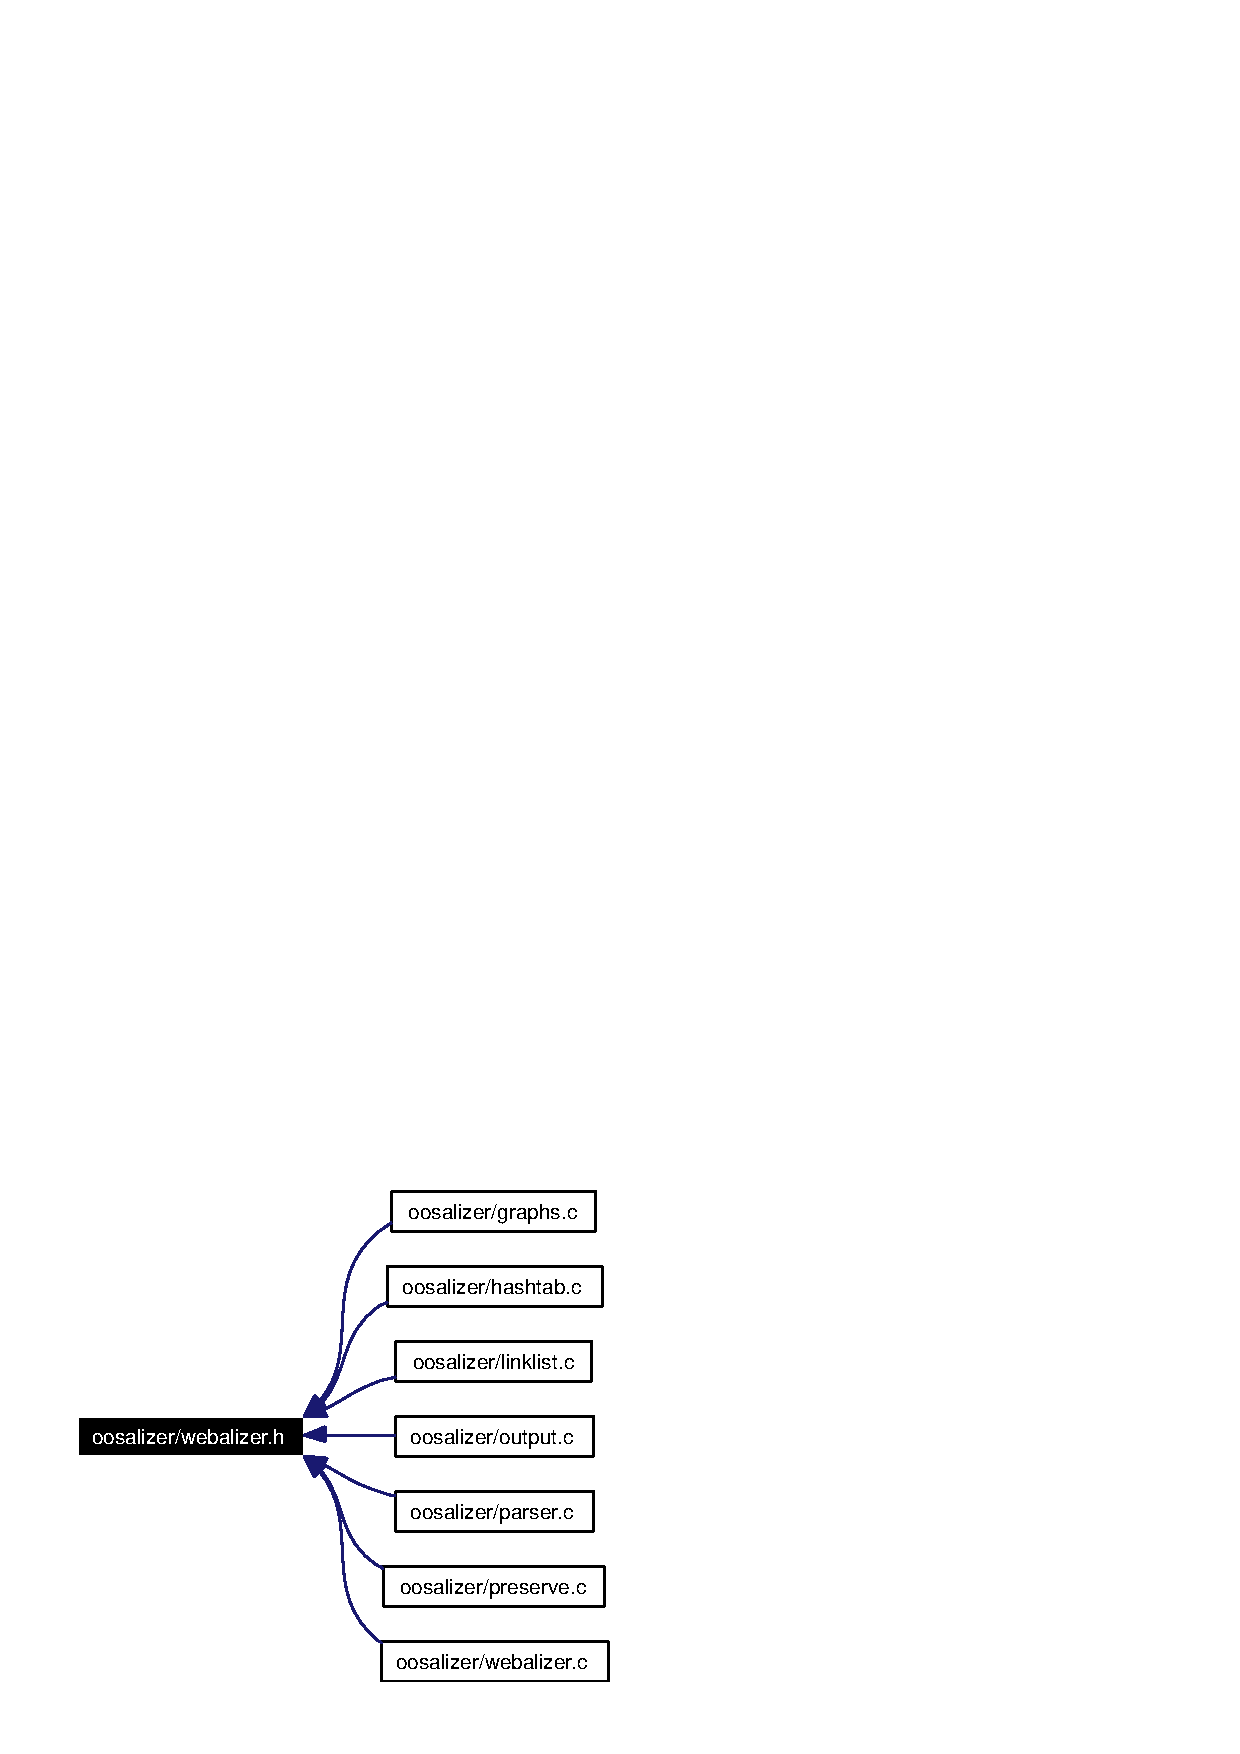
\includegraphics[width=146pt]{webalizer_8h__dep__incl}
\end{center}
\end{figure}
\subsection*{Datenstrukturen}
\begin{CompactItemize}
\item 
struct {\bf response\_\-code}
\item 
struct {\bf response\_\-url}
\item 
struct {\bf responsetmp\_\-url}
\item 
struct {\bf country\_\-code}
\item 
struct {\bf log\_\-struct}
\end{CompactItemize}
\subsection*{Makrodefinitionen}
\begin{CompactItemize}
\item 
\#define {\bf PCENT}(val, max)~((val)?((double)val/(double)max)$\ast$100.0 : 0.0)
\item 
\#define {\bf IDX\_\-2C}(c1, c2)~(((c1-'a'+1)$<$$<$5)+(c2-'a'+1) )
\item 
\#define {\bf IDX\_\-3C}(c1, c2, c3)~(((c1-'a'+1)$<$$<$10)+((c2-'a'+1)$<$$<$5)+(c3-'a'+1) )
\item 
\#define {\bf IDX\_\-4C}(c1, c2, c3, c4)~(((c1-'a'+1)$<$$<$15)+((c2-'a'+1)$<$$<$10)+((c3-'a'+1)$<$$<$5)+(c4-'a'+1) )
\item 
\#define {\bf MAX}(a, b)~((a) $>$ (b) ? (a) : (b))
\item 
\#define {\bf MAXRESP}~1000
\item 
\#define {\bf INCRESP}~500
\item 
\#define {\bf MAXHASH}~2048
\item 
\#define {\bf BUFSIZE}~4096
\item 
\#define {\bf MAXHOST}~128
\item 
\#define {\bf MAXURL}~2048
\item 
\#define {\bf MAXURLH}~512
\item 
\#define {\bf MAXREF}~2048
\item 
\#define {\bf MAXREFH}~512
\item 
\#define {\bf MAXAGENT}~512
\item 
\#define {\bf MAXCTRY}~48
\item 
\#define {\bf MAXSRCH}~512
\item 
\#define {\bf MAXSRCHH}~128
\item 
\#define {\bf MAXIDENT}~64
\item 
\#define {\bf SLOP\_\-VAL}~3600
\item 
\#define {\bf LOG\_\-CLF}~0
\item 
\#define {\bf LOG\_\-FTP}~1
\item 
\#define {\bf LOG\_\-SQUID}~2
\item 
\#define {\bf RC\_\-CONTINUE}~100
\item 
\#define {\bf RC\_\-SWITCHPROTO}~101
\item 
\#define {\bf RC\_\-OK}~200
\item 
\#define {\bf RC\_\-CREATED}~201
\item 
\#define {\bf RC\_\-ACCEPTED}~202
\item 
\#define {\bf RC\_\-NONAUTHINFO}~203
\item 
\#define {\bf RC\_\-NOCONTENT}~204
\item 
\#define {\bf RC\_\-RESETCONTENT}~205
\item 
\#define {\bf RC\_\-PARTIALCONTENT}~206
\item 
\#define {\bf RC\_\-MULTIPLECHOICES}~300
\item 
\#define {\bf RC\_\-MOVEDPERM}~301
\item 
\#define {\bf RC\_\-MOVEDTEMP}~302
\item 
\#define {\bf RC\_\-SEEOTHER}~303
\item 
\#define {\bf RC\_\-NOMOD}~304
\item 
\#define {\bf RC\_\-USEPROXY}~305
\item 
\#define {\bf RC\_\-MOVEDTEMPORARILY}~307
\item 
\#define {\bf RC\_\-BAD}~400
\item 
\#define {\bf RC\_\-UNAUTH}~401
\item 
\#define {\bf RC\_\-PAYMENTREQ}~402
\item 
\#define {\bf RC\_\-FORBIDDEN}~403
\item 
\#define {\bf RC\_\-NOTFOUND}~404
\item 
\#define {\bf RC\_\-METHODNOTALLOWED}~405
\item 
\#define {\bf RC\_\-NOTACCEPTABLE}~406
\item 
\#define {\bf RC\_\-PROXYAUTHREQ}~407
\item 
\#define {\bf RC\_\-TIMEOUT}~408
\item 
\#define {\bf RC\_\-CONFLICT}~409
\item 
\#define {\bf RC\_\-GONE}~410
\item 
\#define {\bf RC\_\-LENGTHREQ}~411
\item 
\#define {\bf RC\_\-PREFAILED}~412
\item 
\#define {\bf RC\_\-REQENTTOOLARGE}~413
\item 
\#define {\bf RC\_\-REQURITOOLARGE}~414
\item 
\#define {\bf RC\_\-UNSUPMEDIATYPE}~415
\item 
\#define {\bf RC\_\-RNGNOTSATISFIABLE}~416
\item 
\#define {\bf RC\_\-EXPECTATIONFAILED}~417
\item 
\#define {\bf RC\_\-SERVERERR}~500
\item 
\#define {\bf RC\_\-NOTIMPLEMENTED}~501
\item 
\#define {\bf RC\_\-BADGATEWAY}~502
\item 
\#define {\bf RC\_\-UNAVAIL}~503
\item 
\#define {\bf RC\_\-GATEWAYTIMEOUT}~504
\item 
\#define {\bf RC\_\-BADHTTPVER}~505
\item 
\#define {\bf IDX\_\-UNDEFINED}~0
\item 
\#define {\bf IDX\_\-CONTINUE}~1
\item 
\#define {\bf IDX\_\-SWITCHPROTO}~2
\item 
\#define {\bf IDX\_\-OK}~3
\item 
\#define {\bf IDX\_\-CREATED}~4
\item 
\#define {\bf IDX\_\-ACCEPTED}~5
\item 
\#define {\bf IDX\_\-NONAUTHINFO}~6
\item 
\#define {\bf IDX\_\-NOCONTENT}~7
\item 
\#define {\bf IDX\_\-RESETCONTENT}~8
\item 
\#define {\bf IDX\_\-PARTIALCONTENT}~9
\item 
\#define {\bf IDX\_\-MULTIPLECHOICES}~10
\item 
\#define {\bf IDX\_\-MOVEDPERM}~11
\item 
\#define {\bf IDX\_\-MOVEDTEMP}~12
\item 
\#define {\bf IDX\_\-SEEOTHER}~13
\item 
\#define {\bf IDX\_\-NOMOD}~14
\item 
\#define {\bf IDX\_\-USEPROXY}~15
\item 
\#define {\bf IDX\_\-MOVEDTEMPORARILY}~16
\item 
\#define {\bf IDX\_\-BAD}~17
\item 
\#define {\bf IDX\_\-UNAUTH}~18
\item 
\#define {\bf IDX\_\-PAYMENTREQ}~19
\item 
\#define {\bf IDX\_\-FORBIDDEN}~20
\item 
\#define {\bf IDX\_\-NOTFOUND}~21
\item 
\#define {\bf IDX\_\-METHODNOTALLOWED}~22
\item 
\#define {\bf IDX\_\-NOTACCEPTABLE}~23
\item 
\#define {\bf IDX\_\-PROXYAUTHREQ}~24
\item 
\#define {\bf IDX\_\-TIMEOUT}~25
\item 
\#define {\bf IDX\_\-CONFLICT}~26
\item 
\#define {\bf IDX\_\-GONE}~27
\item 
\#define {\bf IDX\_\-LENGTHREQ}~28
\item 
\#define {\bf IDX\_\-PREFAILED}~29
\item 
\#define {\bf IDX\_\-REQENTTOOLARGE}~30
\item 
\#define {\bf IDX\_\-REQURITOOLARGE}~31
\item 
\#define {\bf IDX\_\-UNSUPMEDIATYPE}~32
\item 
\#define {\bf IDX\_\-RNGNOTSATISFIABLE}~33
\item 
\#define {\bf IDX\_\-EXPECTATIONFAILED}~34
\item 
\#define {\bf IDX\_\-SERVERERR}~35
\item 
\#define {\bf IDX\_\-NOTIMPLEMENTED}~36
\item 
\#define {\bf IDX\_\-BADGATEWAY}~37
\item 
\#define {\bf IDX\_\-UNAVAIL}~38
\item 
\#define {\bf IDX\_\-GATEWAYTIMEOUT}~39
\item 
\#define {\bf IDX\_\-BADHTTPVER}~40
\item 
\#define {\bf TOTAL\_\-RC}~41
\end{CompactItemize}
\subsection*{Typdefinitionen}
\begin{CompactItemize}
\item 
typedef {\bf country\_\-code} $\ast$ {\bf CLISTPTR}
\end{CompactItemize}
\subsection*{Funktionen}
\begin{CompactItemize}
\item 
char $\ast$ {\bf cur\_\-time} ()
\item 
u\_\-long {\bf ctry\_\-idx} (char $\ast$)
\item 
void {\bf init\_\-counters} ()
\item 
int {\bf ispage} (char $\ast$)
\item 
u\_\-long {\bf jdate} (int, int, int)
\end{CompactItemize}
\subsection*{Variablen}
\begin{CompactItemize}
\item 
{\bf response\_\-url} $\ast$ {\bf respnotfound}
\item 
{\bf responsetmp\_\-url} $\ast$ {\bf respnotfoundtmp}
\item 
u\_\-long {\bf resp\_\-counter}
\item 
{\bf log\_\-struct} {\bf log\_\-rec}
\item 
char $\ast$ {\bf version}
\item 
char $\ast$ {\bf editlvl}
\item 
char $\ast$ {\bf moddate}
\item 
char $\ast$ {\bf copyright}
\item 
int {\bf verbose}
\item 
int {\bf debug\_\-mode}
\item 
int {\bf time\_\-me}
\item 
int {\bf local\_\-time}
\item 
int {\bf ignore\_\-hist}
\item 
int {\bf hourly\_\-graph}
\item 
int {\bf hourly\_\-stats}
\item 
int {\bf daily\_\-graph}
\item 
int {\bf daily\_\-stats}
\item 
int {\bf ctry\_\-graph}
\item 
int {\bf shade\_\-groups}
\item 
int {\bf hlite\_\-groups}
\item 
int {\bf mangle\_\-agent}
\item 
int {\bf incremental}
\item 
int {\bf use\_\-https}
\item 
int {\bf visit\_\-timeout}
\item 
int {\bf graph\_\-legend}
\item 
int {\bf graph\_\-lines}
\item 
int {\bf fold\_\-seq\_\-err}
\item 
int {\bf log\_\-type}
\item 
int {\bf group\_\-domains}
\item 
int {\bf hide\_\-sites}
\item 
char $\ast$ {\bf hname}
\item 
char $\ast$ {\bf state\_\-fname}
\item 
char $\ast$ {\bf hist\_\-fname}
\item 
char $\ast$ {\bf html\_\-ext}
\item 
char $\ast$ {\bf dump\_\-ext}
\item 
char $\ast$ {\bf conf\_\-fname}
\item 
char $\ast$ {\bf log\_\-fname}
\item 
char $\ast$ {\bf out\_\-dir}
\item 
char $\ast$ {\bf blank\_\-str}
\item 
char $\ast$ {\bf dns\_\-cache}
\item 
int {\bf dns\_\-children}
\item 
int {\bf ntop\_\-sites}
\item 
int {\bf ntop\_\-sites\-K}
\item 
int {\bf ntop\_\-urls}
\item 
int {\bf ntop\_\-urls\-K}
\item 
int {\bf ntop\_\-entry}
\item 
int {\bf ntop\_\-exit}
\item 
int {\bf ntop\_\-refs}
\item 
int {\bf ntop\_\-agents}
\item 
int {\bf ntop\_\-ctrys}
\item 
int {\bf ntop\_\-search}
\item 
int {\bf ntop\_\-users}
\item 
int {\bf ntop\_\-notfound}
\item 
int {\bf all\_\-sites}
\item 
int {\bf all\_\-urls}
\item 
int {\bf all\_\-refs}
\item 
int {\bf all\_\-agents}
\item 
int {\bf all\_\-search}
\item 
int {\bf all\_\-users}
\item 
int {\bf dump\_\-sites}
\item 
int {\bf dump\_\-urls}
\item 
int {\bf dump\_\-refs}
\item 
int {\bf dump\_\-agents}
\item 
int {\bf dump\_\-users}
\item 
int {\bf dump\_\-search}
\item 
int {\bf dump\_\-header}
\item 
char $\ast$ {\bf dump\_\-path}
\item 
u\_\-long {\bf cur\_\-tstamp}
\item 
u\_\-long {\bf epoch}
\item 
int {\bf check\_\-dup}
\item 
int {\bf cur\_\-year}
\item 
int {\bf cur\_\-month}
\item 
int {\bf cur\_\-day}
\item 
int {\bf cur\_\-hour}
\item 
int {\bf cur\_\-min}
\item 
int {\bf cur\_\-sec}
\item 
double {\bf t\_\-xfer}
\item 
u\_\-long {\bf t\_\-hit}
\item 
u\_\-long {\bf t\_\-file}
\item 
u\_\-long {\bf t\_\-site}
\item 
u\_\-long {\bf t\_\-url}
\item 
u\_\-long {\bf t\_\-ref}
\item 
u\_\-long {\bf t\_\-agent}
\item 
u\_\-long {\bf t\_\-page}
\item 
u\_\-long {\bf t\_\-visit}
\item 
u\_\-long {\bf t\_\-user}
\item 
double {\bf tm\_\-xfer} [31]
\item 
u\_\-long {\bf tm\_\-hit} [31]
\item 
u\_\-long {\bf tm\_\-file} [31]
\item 
u\_\-long {\bf tm\_\-site} [31]
\item 
u\_\-long {\bf tm\_\-page} [31]
\item 
u\_\-long {\bf tm\_\-visit} [31]
\item 
u\_\-long {\bf dt\_\-site}
\item 
u\_\-long {\bf ht\_\-hit}
\item 
u\_\-long {\bf mh\_\-hit}
\item 
u\_\-long {\bf th\_\-hit} [24]
\item 
u\_\-long {\bf th\_\-file} [24]
\item 
u\_\-long {\bf th\_\-page} [24]
\item 
double {\bf th\_\-xfer} [24]
\item 
int {\bf f\_\-day}
\item 
int {\bf l\_\-day}
\item 
int {\bf gz\_\-log}
\item 
{\bf CLISTPTR} $\ast$ {\bf top\_\-ctrys}
\end{CompactItemize}


\subsection{Makro-Dokumentation}
\index{webalizer.h@{webalizer.h}!BUFSIZE@{BUFSIZE}}
\index{BUFSIZE@{BUFSIZE}!webalizer.h@{webalizer.h}}
\subsubsection{\setlength{\rightskip}{0pt plus 5cm}\#define BUFSIZE~4096}\label{webalizer_8h_eca034f67218340ecb2261a22c2f3dcd}




Definiert in Zeile 16 der Datei webalizer.h.

Wird benutzt von get\_\-config(), get\_\-history(), restore\_\-state(), save\_\-state(), srch\_\-string(), write\_\-main\_\-index() und write\_\-month\_\-html().\index{webalizer.h@{webalizer.h}!IDX_2C@{IDX\_\-2C}}
\index{IDX_2C@{IDX\_\-2C}!webalizer.h@{webalizer.h}}
\subsubsection{\setlength{\rightskip}{0pt plus 5cm}\#define IDX\_\-2C(c1, c2)~(((c1-'a'+1)$<$$<$5)+(c2-'a'+1) )}\label{webalizer_8h_4e6c8a23bbe623659548c4b567bb06df}




Definiert in Zeile 5 der Datei webalizer.h.\index{webalizer.h@{webalizer.h}!IDX_3C@{IDX\_\-3C}}
\index{IDX_3C@{IDX\_\-3C}!webalizer.h@{webalizer.h}}
\subsubsection{\setlength{\rightskip}{0pt plus 5cm}\#define IDX\_\-3C(c1, c2, c3)~(((c1-'a'+1)$<$$<$10)+((c2-'a'+1)$<$$<$5)+(c3-'a'+1) )}\label{webalizer_8h_d70b6fe1fe6cb2c356bbc8268ad87774}




Definiert in Zeile 6 der Datei webalizer.h.\index{webalizer.h@{webalizer.h}!IDX_4C@{IDX\_\-4C}}
\index{IDX_4C@{IDX\_\-4C}!webalizer.h@{webalizer.h}}
\subsubsection{\setlength{\rightskip}{0pt plus 5cm}\#define IDX\_\-4C(c1, c2, c3, c4)~(((c1-'a'+1)$<$$<$15)+((c2-'a'+1)$<$$<$10)+((c3-'a'+1)$<$$<$5)+(c4-'a'+1) )}\label{webalizer_8h_250c884e24a342d554caefc036bf27c1}




Definiert in Zeile 7 der Datei webalizer.h.\index{webalizer.h@{webalizer.h}!IDX_ACCEPTED@{IDX\_\-ACCEPTED}}
\index{IDX_ACCEPTED@{IDX\_\-ACCEPTED}!webalizer.h@{webalizer.h}}
\subsubsection{\setlength{\rightskip}{0pt plus 5cm}\#define IDX\_\-ACCEPTED~5}\label{webalizer_8h_933e0eb54658be0ad274c542b96b143d}




Definiert in Zeile 83 der Datei webalizer.h.\index{webalizer.h@{webalizer.h}!IDX_BAD@{IDX\_\-BAD}}
\index{IDX_BAD@{IDX\_\-BAD}!webalizer.h@{webalizer.h}}
\subsubsection{\setlength{\rightskip}{0pt plus 5cm}\#define IDX\_\-BAD~17}\label{webalizer_8h_48260339557cf3534665eb05912a1868}




Definiert in Zeile 95 der Datei webalizer.h.\index{webalizer.h@{webalizer.h}!IDX_BADGATEWAY@{IDX\_\-BADGATEWAY}}
\index{IDX_BADGATEWAY@{IDX\_\-BADGATEWAY}!webalizer.h@{webalizer.h}}
\subsubsection{\setlength{\rightskip}{0pt plus 5cm}\#define IDX\_\-BADGATEWAY~37}\label{webalizer_8h_2de048827e8a84dab33a5421e9eb2819}




Definiert in Zeile 115 der Datei webalizer.h.\index{webalizer.h@{webalizer.h}!IDX_BADHTTPVER@{IDX\_\-BADHTTPVER}}
\index{IDX_BADHTTPVER@{IDX\_\-BADHTTPVER}!webalizer.h@{webalizer.h}}
\subsubsection{\setlength{\rightskip}{0pt plus 5cm}\#define IDX\_\-BADHTTPVER~40}\label{webalizer_8h_e4191d0093c406af5911ea618427431c}




Definiert in Zeile 118 der Datei webalizer.h.\index{webalizer.h@{webalizer.h}!IDX_CONFLICT@{IDX\_\-CONFLICT}}
\index{IDX_CONFLICT@{IDX\_\-CONFLICT}!webalizer.h@{webalizer.h}}
\subsubsection{\setlength{\rightskip}{0pt plus 5cm}\#define IDX\_\-CONFLICT~26}\label{webalizer_8h_80993fd20ef234e37cd81707101a93e5}




Definiert in Zeile 104 der Datei webalizer.h.\index{webalizer.h@{webalizer.h}!IDX_CONTINUE@{IDX\_\-CONTINUE}}
\index{IDX_CONTINUE@{IDX\_\-CONTINUE}!webalizer.h@{webalizer.h}}
\subsubsection{\setlength{\rightskip}{0pt plus 5cm}\#define IDX\_\-CONTINUE~1}\label{webalizer_8h_83ecb43db7919a2df7837349bbb39e87}




Definiert in Zeile 79 der Datei webalizer.h.\index{webalizer.h@{webalizer.h}!IDX_CREATED@{IDX\_\-CREATED}}
\index{IDX_CREATED@{IDX\_\-CREATED}!webalizer.h@{webalizer.h}}
\subsubsection{\setlength{\rightskip}{0pt plus 5cm}\#define IDX\_\-CREATED~4}\label{webalizer_8h_d4e7a4a0de3d9e8f8fd702d4cc107e5c}




Definiert in Zeile 82 der Datei webalizer.h.\index{webalizer.h@{webalizer.h}!IDX_EXPECTATIONFAILED@{IDX\_\-EXPECTATIONFAILED}}
\index{IDX_EXPECTATIONFAILED@{IDX\_\-EXPECTATIONFAILED}!webalizer.h@{webalizer.h}}
\subsubsection{\setlength{\rightskip}{0pt plus 5cm}\#define IDX\_\-EXPECTATIONFAILED~34}\label{webalizer_8h_31802e28bbe27706459b6d1a9649cebb}




Definiert in Zeile 112 der Datei webalizer.h.\index{webalizer.h@{webalizer.h}!IDX_FORBIDDEN@{IDX\_\-FORBIDDEN}}
\index{IDX_FORBIDDEN@{IDX\_\-FORBIDDEN}!webalizer.h@{webalizer.h}}
\subsubsection{\setlength{\rightskip}{0pt plus 5cm}\#define IDX\_\-FORBIDDEN~20}\label{webalizer_8h_b7b99408c850493c8014826e8bb2c6f3}




Definiert in Zeile 98 der Datei webalizer.h.\index{webalizer.h@{webalizer.h}!IDX_GATEWAYTIMEOUT@{IDX\_\-GATEWAYTIMEOUT}}
\index{IDX_GATEWAYTIMEOUT@{IDX\_\-GATEWAYTIMEOUT}!webalizer.h@{webalizer.h}}
\subsubsection{\setlength{\rightskip}{0pt plus 5cm}\#define IDX\_\-GATEWAYTIMEOUT~39}\label{webalizer_8h_4b7b0e69b67e440b46ddc4c2b9cee01a}




Definiert in Zeile 117 der Datei webalizer.h.\index{webalizer.h@{webalizer.h}!IDX_GONE@{IDX\_\-GONE}}
\index{IDX_GONE@{IDX\_\-GONE}!webalizer.h@{webalizer.h}}
\subsubsection{\setlength{\rightskip}{0pt plus 5cm}\#define IDX\_\-GONE~27}\label{webalizer_8h_016b0abec5b38a6587c1efdc0220b768}




Definiert in Zeile 105 der Datei webalizer.h.\index{webalizer.h@{webalizer.h}!IDX_LENGTHREQ@{IDX\_\-LENGTHREQ}}
\index{IDX_LENGTHREQ@{IDX\_\-LENGTHREQ}!webalizer.h@{webalizer.h}}
\subsubsection{\setlength{\rightskip}{0pt plus 5cm}\#define IDX\_\-LENGTHREQ~28}\label{webalizer_8h_81cd1be9f15877380c00d1c71bd511ff}




Definiert in Zeile 106 der Datei webalizer.h.\index{webalizer.h@{webalizer.h}!IDX_METHODNOTALLOWED@{IDX\_\-METHODNOTALLOWED}}
\index{IDX_METHODNOTALLOWED@{IDX\_\-METHODNOTALLOWED}!webalizer.h@{webalizer.h}}
\subsubsection{\setlength{\rightskip}{0pt plus 5cm}\#define IDX\_\-METHODNOTALLOWED~22}\label{webalizer_8h_41fb3f3f6b1da41411b493a2dd061beb}




Definiert in Zeile 100 der Datei webalizer.h.\index{webalizer.h@{webalizer.h}!IDX_MOVEDPERM@{IDX\_\-MOVEDPERM}}
\index{IDX_MOVEDPERM@{IDX\_\-MOVEDPERM}!webalizer.h@{webalizer.h}}
\subsubsection{\setlength{\rightskip}{0pt plus 5cm}\#define IDX\_\-MOVEDPERM~11}\label{webalizer_8h_dfb37d5b32200232d0b76ecea8f26c84}




Definiert in Zeile 89 der Datei webalizer.h.\index{webalizer.h@{webalizer.h}!IDX_MOVEDTEMP@{IDX\_\-MOVEDTEMP}}
\index{IDX_MOVEDTEMP@{IDX\_\-MOVEDTEMP}!webalizer.h@{webalizer.h}}
\subsubsection{\setlength{\rightskip}{0pt plus 5cm}\#define IDX\_\-MOVEDTEMP~12}\label{webalizer_8h_f6cbf62366bb52a3609fd1e37f9cda52}




Definiert in Zeile 90 der Datei webalizer.h.\index{webalizer.h@{webalizer.h}!IDX_MOVEDTEMPORARILY@{IDX\_\-MOVEDTEMPORARILY}}
\index{IDX_MOVEDTEMPORARILY@{IDX\_\-MOVEDTEMPORARILY}!webalizer.h@{webalizer.h}}
\subsubsection{\setlength{\rightskip}{0pt plus 5cm}\#define IDX\_\-MOVEDTEMPORARILY~16}\label{webalizer_8h_93c6942088e638bf6e98b953d9f2d1f7}




Definiert in Zeile 94 der Datei webalizer.h.\index{webalizer.h@{webalizer.h}!IDX_MULTIPLECHOICES@{IDX\_\-MULTIPLECHOICES}}
\index{IDX_MULTIPLECHOICES@{IDX\_\-MULTIPLECHOICES}!webalizer.h@{webalizer.h}}
\subsubsection{\setlength{\rightskip}{0pt plus 5cm}\#define IDX\_\-MULTIPLECHOICES~10}\label{webalizer_8h_6f4595e5a6403777c1e6cb5831206156}




Definiert in Zeile 88 der Datei webalizer.h.\index{webalizer.h@{webalizer.h}!IDX_NOCONTENT@{IDX\_\-NOCONTENT}}
\index{IDX_NOCONTENT@{IDX\_\-NOCONTENT}!webalizer.h@{webalizer.h}}
\subsubsection{\setlength{\rightskip}{0pt plus 5cm}\#define IDX\_\-NOCONTENT~7}\label{webalizer_8h_56130b6b2cce89fee3bd155d7697792a}




Definiert in Zeile 85 der Datei webalizer.h.\index{webalizer.h@{webalizer.h}!IDX_NOMOD@{IDX\_\-NOMOD}}
\index{IDX_NOMOD@{IDX\_\-NOMOD}!webalizer.h@{webalizer.h}}
\subsubsection{\setlength{\rightskip}{0pt plus 5cm}\#define IDX\_\-NOMOD~14}\label{webalizer_8h_9bfe7536dafc3a3c706d948d72807a3a}




Definiert in Zeile 92 der Datei webalizer.h.\index{webalizer.h@{webalizer.h}!IDX_NONAUTHINFO@{IDX\_\-NONAUTHINFO}}
\index{IDX_NONAUTHINFO@{IDX\_\-NONAUTHINFO}!webalizer.h@{webalizer.h}}
\subsubsection{\setlength{\rightskip}{0pt plus 5cm}\#define IDX\_\-NONAUTHINFO~6}\label{webalizer_8h_939fa36123980dca45b09a9c642c45b4}




Definiert in Zeile 84 der Datei webalizer.h.\index{webalizer.h@{webalizer.h}!IDX_NOTACCEPTABLE@{IDX\_\-NOTACCEPTABLE}}
\index{IDX_NOTACCEPTABLE@{IDX\_\-NOTACCEPTABLE}!webalizer.h@{webalizer.h}}
\subsubsection{\setlength{\rightskip}{0pt plus 5cm}\#define IDX\_\-NOTACCEPTABLE~23}\label{webalizer_8h_beee00b54b28f24ee992a5ccd3107c1c}




Definiert in Zeile 101 der Datei webalizer.h.\index{webalizer.h@{webalizer.h}!IDX_NOTFOUND@{IDX\_\-NOTFOUND}}
\index{IDX_NOTFOUND@{IDX\_\-NOTFOUND}!webalizer.h@{webalizer.h}}
\subsubsection{\setlength{\rightskip}{0pt plus 5cm}\#define IDX\_\-NOTFOUND~21}\label{webalizer_8h_e54d154c414e589efe8192c8207d2839}




Definiert in Zeile 99 der Datei webalizer.h.\index{webalizer.h@{webalizer.h}!IDX_NOTIMPLEMENTED@{IDX\_\-NOTIMPLEMENTED}}
\index{IDX_NOTIMPLEMENTED@{IDX\_\-NOTIMPLEMENTED}!webalizer.h@{webalizer.h}}
\subsubsection{\setlength{\rightskip}{0pt plus 5cm}\#define IDX\_\-NOTIMPLEMENTED~36}\label{webalizer_8h_7ed773dca0aac3af7eb48e70d7483ebb}




Definiert in Zeile 114 der Datei webalizer.h.\index{webalizer.h@{webalizer.h}!IDX_OK@{IDX\_\-OK}}
\index{IDX_OK@{IDX\_\-OK}!webalizer.h@{webalizer.h}}
\subsubsection{\setlength{\rightskip}{0pt plus 5cm}\#define IDX\_\-OK~3}\label{webalizer_8h_8414d7b1864c34564ece4a0bbc184b59}




Definiert in Zeile 81 der Datei webalizer.h.\index{webalizer.h@{webalizer.h}!IDX_PARTIALCONTENT@{IDX\_\-PARTIALCONTENT}}
\index{IDX_PARTIALCONTENT@{IDX\_\-PARTIALCONTENT}!webalizer.h@{webalizer.h}}
\subsubsection{\setlength{\rightskip}{0pt plus 5cm}\#define IDX\_\-PARTIALCONTENT~9}\label{webalizer_8h_781f7d89028f787181cb19ae2467e1fa}




Definiert in Zeile 87 der Datei webalizer.h.\index{webalizer.h@{webalizer.h}!IDX_PAYMENTREQ@{IDX\_\-PAYMENTREQ}}
\index{IDX_PAYMENTREQ@{IDX\_\-PAYMENTREQ}!webalizer.h@{webalizer.h}}
\subsubsection{\setlength{\rightskip}{0pt plus 5cm}\#define IDX\_\-PAYMENTREQ~19}\label{webalizer_8h_aa47991200d3a366985009e68b0f24a0}




Definiert in Zeile 97 der Datei webalizer.h.\index{webalizer.h@{webalizer.h}!IDX_PREFAILED@{IDX\_\-PREFAILED}}
\index{IDX_PREFAILED@{IDX\_\-PREFAILED}!webalizer.h@{webalizer.h}}
\subsubsection{\setlength{\rightskip}{0pt plus 5cm}\#define IDX\_\-PREFAILED~29}\label{webalizer_8h_dd268ced3960a37e6f03794d754d37c4}




Definiert in Zeile 107 der Datei webalizer.h.\index{webalizer.h@{webalizer.h}!IDX_PROXYAUTHREQ@{IDX\_\-PROXYAUTHREQ}}
\index{IDX_PROXYAUTHREQ@{IDX\_\-PROXYAUTHREQ}!webalizer.h@{webalizer.h}}
\subsubsection{\setlength{\rightskip}{0pt plus 5cm}\#define IDX\_\-PROXYAUTHREQ~24}\label{webalizer_8h_2512abf4bfb02560c15b69fbb96f1116}




Definiert in Zeile 102 der Datei webalizer.h.\index{webalizer.h@{webalizer.h}!IDX_REQENTTOOLARGE@{IDX\_\-REQENTTOOLARGE}}
\index{IDX_REQENTTOOLARGE@{IDX\_\-REQENTTOOLARGE}!webalizer.h@{webalizer.h}}
\subsubsection{\setlength{\rightskip}{0pt plus 5cm}\#define IDX\_\-REQENTTOOLARGE~30}\label{webalizer_8h_800af5d850306ceda4230bc357eb49a1}




Definiert in Zeile 108 der Datei webalizer.h.\index{webalizer.h@{webalizer.h}!IDX_REQURITOOLARGE@{IDX\_\-REQURITOOLARGE}}
\index{IDX_REQURITOOLARGE@{IDX\_\-REQURITOOLARGE}!webalizer.h@{webalizer.h}}
\subsubsection{\setlength{\rightskip}{0pt plus 5cm}\#define IDX\_\-REQURITOOLARGE~31}\label{webalizer_8h_2ff00bc5fadae34827ff0514047124b4}




Definiert in Zeile 109 der Datei webalizer.h.\index{webalizer.h@{webalizer.h}!IDX_RESETCONTENT@{IDX\_\-RESETCONTENT}}
\index{IDX_RESETCONTENT@{IDX\_\-RESETCONTENT}!webalizer.h@{webalizer.h}}
\subsubsection{\setlength{\rightskip}{0pt plus 5cm}\#define IDX\_\-RESETCONTENT~8}\label{webalizer_8h_06fdfc6a30a2c0e48f0f5e4aa47064c9}




Definiert in Zeile 86 der Datei webalizer.h.\index{webalizer.h@{webalizer.h}!IDX_RNGNOTSATISFIABLE@{IDX\_\-RNGNOTSATISFIABLE}}
\index{IDX_RNGNOTSATISFIABLE@{IDX\_\-RNGNOTSATISFIABLE}!webalizer.h@{webalizer.h}}
\subsubsection{\setlength{\rightskip}{0pt plus 5cm}\#define IDX\_\-RNGNOTSATISFIABLE~33}\label{webalizer_8h_5aafa8994d729c3cbcc7c6564ee32793}




Definiert in Zeile 111 der Datei webalizer.h.\index{webalizer.h@{webalizer.h}!IDX_SEEOTHER@{IDX\_\-SEEOTHER}}
\index{IDX_SEEOTHER@{IDX\_\-SEEOTHER}!webalizer.h@{webalizer.h}}
\subsubsection{\setlength{\rightskip}{0pt plus 5cm}\#define IDX\_\-SEEOTHER~13}\label{webalizer_8h_7e2706d21cedca3fe0b354d5a1ead818}




Definiert in Zeile 91 der Datei webalizer.h.\index{webalizer.h@{webalizer.h}!IDX_SERVERERR@{IDX\_\-SERVERERR}}
\index{IDX_SERVERERR@{IDX\_\-SERVERERR}!webalizer.h@{webalizer.h}}
\subsubsection{\setlength{\rightskip}{0pt plus 5cm}\#define IDX\_\-SERVERERR~35}\label{webalizer_8h_172077342801961a306c9d7a1fac4433}




Definiert in Zeile 113 der Datei webalizer.h.\index{webalizer.h@{webalizer.h}!IDX_SWITCHPROTO@{IDX\_\-SWITCHPROTO}}
\index{IDX_SWITCHPROTO@{IDX\_\-SWITCHPROTO}!webalizer.h@{webalizer.h}}
\subsubsection{\setlength{\rightskip}{0pt plus 5cm}\#define IDX\_\-SWITCHPROTO~2}\label{webalizer_8h_f75dbc50a390198de5a2b7fa3a1cf74e}




Definiert in Zeile 80 der Datei webalizer.h.\index{webalizer.h@{webalizer.h}!IDX_TIMEOUT@{IDX\_\-TIMEOUT}}
\index{IDX_TIMEOUT@{IDX\_\-TIMEOUT}!webalizer.h@{webalizer.h}}
\subsubsection{\setlength{\rightskip}{0pt plus 5cm}\#define IDX\_\-TIMEOUT~25}\label{webalizer_8h_c6815df17d8a5de1d1d9f2cfebc54549}




Definiert in Zeile 103 der Datei webalizer.h.\index{webalizer.h@{webalizer.h}!IDX_UNAUTH@{IDX\_\-UNAUTH}}
\index{IDX_UNAUTH@{IDX\_\-UNAUTH}!webalizer.h@{webalizer.h}}
\subsubsection{\setlength{\rightskip}{0pt plus 5cm}\#define IDX\_\-UNAUTH~18}\label{webalizer_8h_8ea05eb3e8a1b38e57de383d26c37504}




Definiert in Zeile 96 der Datei webalizer.h.\index{webalizer.h@{webalizer.h}!IDX_UNAVAIL@{IDX\_\-UNAVAIL}}
\index{IDX_UNAVAIL@{IDX\_\-UNAVAIL}!webalizer.h@{webalizer.h}}
\subsubsection{\setlength{\rightskip}{0pt plus 5cm}\#define IDX\_\-UNAVAIL~38}\label{webalizer_8h_e22b7bcbc25b5d27c2f17f513e5fb470}




Definiert in Zeile 116 der Datei webalizer.h.\index{webalizer.h@{webalizer.h}!IDX_UNDEFINED@{IDX\_\-UNDEFINED}}
\index{IDX_UNDEFINED@{IDX\_\-UNDEFINED}!webalizer.h@{webalizer.h}}
\subsubsection{\setlength{\rightskip}{0pt plus 5cm}\#define IDX\_\-UNDEFINED~0}\label{webalizer_8h_b93bf51da9eb22f9c1137af150b41875}




Definiert in Zeile 78 der Datei webalizer.h.\index{webalizer.h@{webalizer.h}!IDX_UNSUPMEDIATYPE@{IDX\_\-UNSUPMEDIATYPE}}
\index{IDX_UNSUPMEDIATYPE@{IDX\_\-UNSUPMEDIATYPE}!webalizer.h@{webalizer.h}}
\subsubsection{\setlength{\rightskip}{0pt plus 5cm}\#define IDX\_\-UNSUPMEDIATYPE~32}\label{webalizer_8h_e11d6a0f8e87a7188ecc2d97b40e6027}




Definiert in Zeile 110 der Datei webalizer.h.\index{webalizer.h@{webalizer.h}!IDX_USEPROXY@{IDX\_\-USEPROXY}}
\index{IDX_USEPROXY@{IDX\_\-USEPROXY}!webalizer.h@{webalizer.h}}
\subsubsection{\setlength{\rightskip}{0pt plus 5cm}\#define IDX\_\-USEPROXY~15}\label{webalizer_8h_78d0d675c3de5dae71aa53d872331bc4}




Definiert in Zeile 93 der Datei webalizer.h.\index{webalizer.h@{webalizer.h}!INCRESP@{INCRESP}}
\index{INCRESP@{INCRESP}!webalizer.h@{webalizer.h}}
\subsubsection{\setlength{\rightskip}{0pt plus 5cm}\#define INCRESP~500}\label{webalizer_8h_08a8f937430dfb2f8d178491808565c4}




Definiert in Zeile 14 der Datei webalizer.h.\index{webalizer.h@{webalizer.h}!LOG_CLF@{LOG\_\-CLF}}
\index{LOG_CLF@{LOG\_\-CLF}!webalizer.h@{webalizer.h}}
\subsubsection{\setlength{\rightskip}{0pt plus 5cm}\#define LOG\_\-CLF~0}\label{webalizer_8h_5ce0d49d0e92ba00b7385ef68d26b51a}




Definiert in Zeile 31 der Datei webalizer.h.

Wird benutzt von main() und parse\_\-record().\index{webalizer.h@{webalizer.h}!LOG_FTP@{LOG\_\-FTP}}
\index{LOG_FTP@{LOG\_\-FTP}!webalizer.h@{webalizer.h}}
\subsubsection{\setlength{\rightskip}{0pt plus 5cm}\#define LOG\_\-FTP~1}\label{webalizer_8h_cf5d4c2811adb735aaf5b32f62cc3cea}




Definiert in Zeile 32 der Datei webalizer.h.

Wird benutzt von main(), parse\_\-record() und top\_\-urls\_\-table().\index{webalizer.h@{webalizer.h}!LOG_SQUID@{LOG\_\-SQUID}}
\index{LOG_SQUID@{LOG\_\-SQUID}!webalizer.h@{webalizer.h}}
\subsubsection{\setlength{\rightskip}{0pt plus 5cm}\#define LOG\_\-SQUID~2}\label{webalizer_8h_43821087b540ecbc400b7cef8ab10be0}




Definiert in Zeile 33 der Datei webalizer.h.

Wird benutzt von main() und parse\_\-record().\index{webalizer.h@{webalizer.h}!MAX@{MAX}}
\index{MAX@{MAX}!webalizer.h@{webalizer.h}}
\subsubsection{\setlength{\rightskip}{0pt plus 5cm}\#define MAX(a, b)~((a) $>$ (b) ? (a) : (b))}\label{webalizer_8h_fa99ec4acc4ecb2dc3c2d05da15d0e3f}




Definiert in Zeile 10 der Datei webalizer.h.\index{webalizer.h@{webalizer.h}!MAXAGENT@{MAXAGENT}}
\index{MAXAGENT@{MAXAGENT}!webalizer.h@{webalizer.h}}
\subsubsection{\setlength{\rightskip}{0pt plus 5cm}\#define MAXAGENT~512}\label{webalizer_8h_cac54bd107b23b8a6433b11c185a884d}




Definiert in Zeile 22 der Datei webalizer.h.

Wird benutzt von new\_\-anode() und parse\_\-record\_\-web().\index{webalizer.h@{webalizer.h}!MAXCTRY@{MAXCTRY}}
\index{MAXCTRY@{MAXCTRY}!webalizer.h@{webalizer.h}}
\subsubsection{\setlength{\rightskip}{0pt plus 5cm}\#define MAXCTRY~48}\label{webalizer_8h_1ee34374643e38b0f4ae8fff42539f32}




Definiert in Zeile 23 der Datei webalizer.h.\index{webalizer.h@{webalizer.h}!MAXHASH@{MAXHASH}}
\index{MAXHASH@{MAXHASH}!webalizer.h@{webalizer.h}}
\subsubsection{\setlength{\rightskip}{0pt plus 5cm}\#define MAXHASH~2048}\label{webalizer_8h_381dfed3a446e2b49171f4593a701df8}




Definiert in Zeile 15 der Datei webalizer.h.

Wird benutzt von del\_\-alist(), del\_\-hlist(), del\_\-ilist(), del\_\-rlist(), del\_\-slist(), del\_\-ulist(), load\_\-agent\_\-array(), load\_\-ident\_\-array(), load\_\-ref\_\-array(), load\_\-site\_\-array(), load\_\-srch\_\-array(), load\_\-url\_\-array(), top\_\-ctry\_\-table() und tot\_\-visit().\index{webalizer.h@{webalizer.h}!MAXHOST@{MAXHOST}}
\index{MAXHOST@{MAXHOST}!webalizer.h@{webalizer.h}}
\subsubsection{\setlength{\rightskip}{0pt plus 5cm}\#define MAXHOST~128}\label{webalizer_8h_35a96510c197e5b56b079fd4b85a40d6}




Definiert in Zeile 17 der Datei webalizer.h.

Wird benutzt von new\_\-hnode(), parse\_\-record\_\-ftp(), parse\_\-record\_\-squid() und parse\_\-record\_\-web().\index{webalizer.h@{webalizer.h}!MAXIDENT@{MAXIDENT}}
\index{MAXIDENT@{MAXIDENT}!webalizer.h@{webalizer.h}}
\subsubsection{\setlength{\rightskip}{0pt plus 5cm}\#define MAXIDENT~64}\label{webalizer_8h_f4f5153d8faa075eda9141a6de77764b}




Definiert in Zeile 26 der Datei webalizer.h.

Wird benutzt von new\_\-inode(), parse\_\-record\_\-squid() und parse\_\-record\_\-web().\index{webalizer.h@{webalizer.h}!MAXREF@{MAXREF}}
\index{MAXREF@{MAXREF}!webalizer.h@{webalizer.h}}
\subsubsection{\setlength{\rightskip}{0pt plus 5cm}\#define MAXREF~2048}\label{webalizer_8h_93490f19b31aee2379f0acc0aa08af06}




Definiert in Zeile 20 der Datei webalizer.h.

Wird benutzt von parse\_\-record\_\-web().\index{webalizer.h@{webalizer.h}!MAXREFH@{MAXREFH}}
\index{MAXREFH@{MAXREFH}!webalizer.h@{webalizer.h}}
\subsubsection{\setlength{\rightskip}{0pt plus 5cm}\#define MAXREFH~512}\label{webalizer_8h_2c5b86478207547dbb0f2f026725c8f8}




Definiert in Zeile 21 der Datei webalizer.h.

Wird benutzt von new\_\-rnode().\index{webalizer.h@{webalizer.h}!MAXRESP@{MAXRESP}}
\index{MAXRESP@{MAXRESP}!webalizer.h@{webalizer.h}}
\subsubsection{\setlength{\rightskip}{0pt plus 5cm}\#define MAXRESP~1000}\label{webalizer_8h_3d47d7a8b615ae32d0978491b0fdd2a7}




Definiert in Zeile 13 der Datei webalizer.h.

Wird benutzt von main().\index{webalizer.h@{webalizer.h}!MAXSRCH@{MAXSRCH}}
\index{MAXSRCH@{MAXSRCH}!webalizer.h@{webalizer.h}}
\subsubsection{\setlength{\rightskip}{0pt plus 5cm}\#define MAXSRCH~512}\label{webalizer_8h_fbd0e79f3020d8a6df0a85a2300bbd3c}




Definiert in Zeile 24 der Datei webalizer.h.\index{webalizer.h@{webalizer.h}!MAXSRCHH@{MAXSRCHH}}
\index{MAXSRCHH@{MAXSRCHH}!webalizer.h@{webalizer.h}}
\subsubsection{\setlength{\rightskip}{0pt plus 5cm}\#define MAXSRCHH~128}\label{webalizer_8h_da235f98b7907e34754de783b33f69f1}




Definiert in Zeile 25 der Datei webalizer.h.

Wird benutzt von new\_\-snode().\index{webalizer.h@{webalizer.h}!MAXURL@{MAXURL}}
\index{MAXURL@{MAXURL}!webalizer.h@{webalizer.h}}
\subsubsection{\setlength{\rightskip}{0pt plus 5cm}\#define MAXURL~2048}\label{webalizer_8h_154e43d94122a068e2f1b110ef9885fa}




Definiert in Zeile 18 der Datei webalizer.h.

Wird benutzt von parse\_\-record\_\-ftp(), parse\_\-record\_\-squid() und parse\_\-record\_\-web().\index{webalizer.h@{webalizer.h}!MAXURLH@{MAXURLH}}
\index{MAXURLH@{MAXURLH}!webalizer.h@{webalizer.h}}
\subsubsection{\setlength{\rightskip}{0pt plus 5cm}\#define MAXURLH~512}\label{webalizer_8h_25de11d4cd5b64bfd955e494e2b5d815}




Definiert in Zeile 19 der Datei webalizer.h.

Wird benutzt von new\_\-unode().\index{webalizer.h@{webalizer.h}!PCENT@{PCENT}}
\index{PCENT@{PCENT}!webalizer.h@{webalizer.h}}
\subsubsection{\setlength{\rightskip}{0pt plus 5cm}\#define PCENT(val, max)~((val)?((double)val/(double)max)$\ast$100.0 : 0.0)}\label{webalizer_8h_349ccc58930e23a50f4cdd125a2edf7d}




Definiert in Zeile 4 der Datei webalizer.h.

Wird benutzt von daily\_\-total\_\-table() und hourly\_\-total\_\-table().\index{webalizer.h@{webalizer.h}!RC_ACCEPTED@{RC\_\-ACCEPTED}}
\index{RC_ACCEPTED@{RC\_\-ACCEPTED}!webalizer.h@{webalizer.h}}
\subsubsection{\setlength{\rightskip}{0pt plus 5cm}\#define RC\_\-ACCEPTED~202}\label{webalizer_8h_1dc4c23d4b1d53e2c441c8f0be4a6c8f}




Definiert in Zeile 40 der Datei webalizer.h.\index{webalizer.h@{webalizer.h}!RC_BAD@{RC\_\-BAD}}
\index{RC_BAD@{RC\_\-BAD}!webalizer.h@{webalizer.h}}
\subsubsection{\setlength{\rightskip}{0pt plus 5cm}\#define RC\_\-BAD~400}\label{webalizer_8h_fe7364776d74e37117c140dd2a57120d}




Definiert in Zeile 52 der Datei webalizer.h.\index{webalizer.h@{webalizer.h}!RC_BADGATEWAY@{RC\_\-BADGATEWAY}}
\index{RC_BADGATEWAY@{RC\_\-BADGATEWAY}!webalizer.h@{webalizer.h}}
\subsubsection{\setlength{\rightskip}{0pt plus 5cm}\#define RC\_\-BADGATEWAY~502}\label{webalizer_8h_1d6c4fd6c60fc320baee08a960890fc3}




Definiert in Zeile 72 der Datei webalizer.h.\index{webalizer.h@{webalizer.h}!RC_BADHTTPVER@{RC\_\-BADHTTPVER}}
\index{RC_BADHTTPVER@{RC\_\-BADHTTPVER}!webalizer.h@{webalizer.h}}
\subsubsection{\setlength{\rightskip}{0pt plus 5cm}\#define RC\_\-BADHTTPVER~505}\label{webalizer_8h_97071445bafc08e42f84edfb030bd18e}




Definiert in Zeile 75 der Datei webalizer.h.\index{webalizer.h@{webalizer.h}!RC_CONFLICT@{RC\_\-CONFLICT}}
\index{RC_CONFLICT@{RC\_\-CONFLICT}!webalizer.h@{webalizer.h}}
\subsubsection{\setlength{\rightskip}{0pt plus 5cm}\#define RC\_\-CONFLICT~409}\label{webalizer_8h_de706652b6ba7c52ded58b8945282a10}




Definiert in Zeile 61 der Datei webalizer.h.\index{webalizer.h@{webalizer.h}!RC_CONTINUE@{RC\_\-CONTINUE}}
\index{RC_CONTINUE@{RC\_\-CONTINUE}!webalizer.h@{webalizer.h}}
\subsubsection{\setlength{\rightskip}{0pt plus 5cm}\#define RC\_\-CONTINUE~100}\label{webalizer_8h_2973ef9c3946a53a2d2abb55a55a3b97}




Definiert in Zeile 36 der Datei webalizer.h.\index{webalizer.h@{webalizer.h}!RC_CREATED@{RC\_\-CREATED}}
\index{RC_CREATED@{RC\_\-CREATED}!webalizer.h@{webalizer.h}}
\subsubsection{\setlength{\rightskip}{0pt plus 5cm}\#define RC\_\-CREATED~201}\label{webalizer_8h_f0332079723f3067bbfaaa3898c92f83}




Definiert in Zeile 39 der Datei webalizer.h.\index{webalizer.h@{webalizer.h}!RC_EXPECTATIONFAILED@{RC\_\-EXPECTATIONFAILED}}
\index{RC_EXPECTATIONFAILED@{RC\_\-EXPECTATIONFAILED}!webalizer.h@{webalizer.h}}
\subsubsection{\setlength{\rightskip}{0pt plus 5cm}\#define RC\_\-EXPECTATIONFAILED~417}\label{webalizer_8h_491c8d8e375207b66d0d730c96f7f72f}




Definiert in Zeile 69 der Datei webalizer.h.\index{webalizer.h@{webalizer.h}!RC_FORBIDDEN@{RC\_\-FORBIDDEN}}
\index{RC_FORBIDDEN@{RC\_\-FORBIDDEN}!webalizer.h@{webalizer.h}}
\subsubsection{\setlength{\rightskip}{0pt plus 5cm}\#define RC\_\-FORBIDDEN~403}\label{webalizer_8h_80228f15ff6a244a08c671165772a4cb}




Definiert in Zeile 55 der Datei webalizer.h.\index{webalizer.h@{webalizer.h}!RC_GATEWAYTIMEOUT@{RC\_\-GATEWAYTIMEOUT}}
\index{RC_GATEWAYTIMEOUT@{RC\_\-GATEWAYTIMEOUT}!webalizer.h@{webalizer.h}}
\subsubsection{\setlength{\rightskip}{0pt plus 5cm}\#define RC\_\-GATEWAYTIMEOUT~504}\label{webalizer_8h_9a6769b1960fc266b7276c99ae6be4b4}




Definiert in Zeile 74 der Datei webalizer.h.\index{webalizer.h@{webalizer.h}!RC_GONE@{RC\_\-GONE}}
\index{RC_GONE@{RC\_\-GONE}!webalizer.h@{webalizer.h}}
\subsubsection{\setlength{\rightskip}{0pt plus 5cm}\#define RC\_\-GONE~410}\label{webalizer_8h_e3c00160efe3330657c85c15d047490c}




Definiert in Zeile 62 der Datei webalizer.h.\index{webalizer.h@{webalizer.h}!RC_LENGTHREQ@{RC\_\-LENGTHREQ}}
\index{RC_LENGTHREQ@{RC\_\-LENGTHREQ}!webalizer.h@{webalizer.h}}
\subsubsection{\setlength{\rightskip}{0pt plus 5cm}\#define RC\_\-LENGTHREQ~411}\label{webalizer_8h_d8e34c952fc0f159e05586be6444fd7e}




Definiert in Zeile 63 der Datei webalizer.h.\index{webalizer.h@{webalizer.h}!RC_METHODNOTALLOWED@{RC\_\-METHODNOTALLOWED}}
\index{RC_METHODNOTALLOWED@{RC\_\-METHODNOTALLOWED}!webalizer.h@{webalizer.h}}
\subsubsection{\setlength{\rightskip}{0pt plus 5cm}\#define RC\_\-METHODNOTALLOWED~405}\label{webalizer_8h_aefe9210427876578c52b3d1b9585d26}




Definiert in Zeile 57 der Datei webalizer.h.\index{webalizer.h@{webalizer.h}!RC_MOVEDPERM@{RC\_\-MOVEDPERM}}
\index{RC_MOVEDPERM@{RC\_\-MOVEDPERM}!webalizer.h@{webalizer.h}}
\subsubsection{\setlength{\rightskip}{0pt plus 5cm}\#define RC\_\-MOVEDPERM~301}\label{webalizer_8h_377e76f0029c632db82eeed9ca566170}




Definiert in Zeile 46 der Datei webalizer.h.\index{webalizer.h@{webalizer.h}!RC_MOVEDTEMP@{RC\_\-MOVEDTEMP}}
\index{RC_MOVEDTEMP@{RC\_\-MOVEDTEMP}!webalizer.h@{webalizer.h}}
\subsubsection{\setlength{\rightskip}{0pt plus 5cm}\#define RC\_\-MOVEDTEMP~302}\label{webalizer_8h_c68cd020d1f6ac6c183545ac2ddedac4}




Definiert in Zeile 47 der Datei webalizer.h.\index{webalizer.h@{webalizer.h}!RC_MOVEDTEMPORARILY@{RC\_\-MOVEDTEMPORARILY}}
\index{RC_MOVEDTEMPORARILY@{RC\_\-MOVEDTEMPORARILY}!webalizer.h@{webalizer.h}}
\subsubsection{\setlength{\rightskip}{0pt plus 5cm}\#define RC\_\-MOVEDTEMPORARILY~307}\label{webalizer_8h_f51f0ab3e378b9069e91c0cdb70967f0}




Definiert in Zeile 51 der Datei webalizer.h.\index{webalizer.h@{webalizer.h}!RC_MULTIPLECHOICES@{RC\_\-MULTIPLECHOICES}}
\index{RC_MULTIPLECHOICES@{RC\_\-MULTIPLECHOICES}!webalizer.h@{webalizer.h}}
\subsubsection{\setlength{\rightskip}{0pt plus 5cm}\#define RC\_\-MULTIPLECHOICES~300}\label{webalizer_8h_e57d896ee18e8ef51e3787d3d00227ad}




Definiert in Zeile 45 der Datei webalizer.h.\index{webalizer.h@{webalizer.h}!RC_NOCONTENT@{RC\_\-NOCONTENT}}
\index{RC_NOCONTENT@{RC\_\-NOCONTENT}!webalizer.h@{webalizer.h}}
\subsubsection{\setlength{\rightskip}{0pt plus 5cm}\#define RC\_\-NOCONTENT~204}\label{webalizer_8h_2a4892c2fd090a258e299fe74a2b62bc}




Definiert in Zeile 42 der Datei webalizer.h.\index{webalizer.h@{webalizer.h}!RC_NOMOD@{RC\_\-NOMOD}}
\index{RC_NOMOD@{RC\_\-NOMOD}!webalizer.h@{webalizer.h}}
\subsubsection{\setlength{\rightskip}{0pt plus 5cm}\#define RC\_\-NOMOD~304}\label{webalizer_8h_eff5fe0e9d6e0d3b059e98fa6a7af4c0}




Definiert in Zeile 49 der Datei webalizer.h.\index{webalizer.h@{webalizer.h}!RC_NONAUTHINFO@{RC\_\-NONAUTHINFO}}
\index{RC_NONAUTHINFO@{RC\_\-NONAUTHINFO}!webalizer.h@{webalizer.h}}
\subsubsection{\setlength{\rightskip}{0pt plus 5cm}\#define RC\_\-NONAUTHINFO~203}\label{webalizer_8h_8ecd21218957eab5e7e58325f40f6552}




Definiert in Zeile 41 der Datei webalizer.h.\index{webalizer.h@{webalizer.h}!RC_NOTACCEPTABLE@{RC\_\-NOTACCEPTABLE}}
\index{RC_NOTACCEPTABLE@{RC\_\-NOTACCEPTABLE}!webalizer.h@{webalizer.h}}
\subsubsection{\setlength{\rightskip}{0pt plus 5cm}\#define RC\_\-NOTACCEPTABLE~406}\label{webalizer_8h_84e1c25114a994a902bcc647855ac889}




Definiert in Zeile 58 der Datei webalizer.h.\index{webalizer.h@{webalizer.h}!RC_NOTFOUND@{RC\_\-NOTFOUND}}
\index{RC_NOTFOUND@{RC\_\-NOTFOUND}!webalizer.h@{webalizer.h}}
\subsubsection{\setlength{\rightskip}{0pt plus 5cm}\#define RC\_\-NOTFOUND~404}\label{webalizer_8h_71678208a421e84056782803d8a4b123}




Definiert in Zeile 56 der Datei webalizer.h.\index{webalizer.h@{webalizer.h}!RC_NOTIMPLEMENTED@{RC\_\-NOTIMPLEMENTED}}
\index{RC_NOTIMPLEMENTED@{RC\_\-NOTIMPLEMENTED}!webalizer.h@{webalizer.h}}
\subsubsection{\setlength{\rightskip}{0pt plus 5cm}\#define RC\_\-NOTIMPLEMENTED~501}\label{webalizer_8h_ede48bc0a06917580753201049f9e396}




Definiert in Zeile 71 der Datei webalizer.h.\index{webalizer.h@{webalizer.h}!RC_OK@{RC\_\-OK}}
\index{RC_OK@{RC\_\-OK}!webalizer.h@{webalizer.h}}
\subsubsection{\setlength{\rightskip}{0pt plus 5cm}\#define RC\_\-OK~200}\label{webalizer_8h_c96a9e3f6c17299d532eb572ef0ea415}




Definiert in Zeile 38 der Datei webalizer.h.\index{webalizer.h@{webalizer.h}!RC_PARTIALCONTENT@{RC\_\-PARTIALCONTENT}}
\index{RC_PARTIALCONTENT@{RC\_\-PARTIALCONTENT}!webalizer.h@{webalizer.h}}
\subsubsection{\setlength{\rightskip}{0pt plus 5cm}\#define RC\_\-PARTIALCONTENT~206}\label{webalizer_8h_893e07be696874c598cea81950e6c072}




Definiert in Zeile 44 der Datei webalizer.h.\index{webalizer.h@{webalizer.h}!RC_PAYMENTREQ@{RC\_\-PAYMENTREQ}}
\index{RC_PAYMENTREQ@{RC\_\-PAYMENTREQ}!webalizer.h@{webalizer.h}}
\subsubsection{\setlength{\rightskip}{0pt plus 5cm}\#define RC\_\-PAYMENTREQ~402}\label{webalizer_8h_632840a368cc8995b7cf7c5a2a8fcae9}




Definiert in Zeile 54 der Datei webalizer.h.\index{webalizer.h@{webalizer.h}!RC_PREFAILED@{RC\_\-PREFAILED}}
\index{RC_PREFAILED@{RC\_\-PREFAILED}!webalizer.h@{webalizer.h}}
\subsubsection{\setlength{\rightskip}{0pt plus 5cm}\#define RC\_\-PREFAILED~412}\label{webalizer_8h_1b9f678bdf687297ee1d2c6d33901a9d}




Definiert in Zeile 64 der Datei webalizer.h.\index{webalizer.h@{webalizer.h}!RC_PROXYAUTHREQ@{RC\_\-PROXYAUTHREQ}}
\index{RC_PROXYAUTHREQ@{RC\_\-PROXYAUTHREQ}!webalizer.h@{webalizer.h}}
\subsubsection{\setlength{\rightskip}{0pt plus 5cm}\#define RC\_\-PROXYAUTHREQ~407}\label{webalizer_8h_bb3cc66b80375945009d866c67106eec}




Definiert in Zeile 59 der Datei webalizer.h.\index{webalizer.h@{webalizer.h}!RC_REQENTTOOLARGE@{RC\_\-REQENTTOOLARGE}}
\index{RC_REQENTTOOLARGE@{RC\_\-REQENTTOOLARGE}!webalizer.h@{webalizer.h}}
\subsubsection{\setlength{\rightskip}{0pt plus 5cm}\#define RC\_\-REQENTTOOLARGE~413}\label{webalizer_8h_09481992e00a806a61fa09aa85ba914a}




Definiert in Zeile 65 der Datei webalizer.h.\index{webalizer.h@{webalizer.h}!RC_REQURITOOLARGE@{RC\_\-REQURITOOLARGE}}
\index{RC_REQURITOOLARGE@{RC\_\-REQURITOOLARGE}!webalizer.h@{webalizer.h}}
\subsubsection{\setlength{\rightskip}{0pt plus 5cm}\#define RC\_\-REQURITOOLARGE~414}\label{webalizer_8h_94a11e7b21ac575205e9100b72e23d8d}




Definiert in Zeile 66 der Datei webalizer.h.\index{webalizer.h@{webalizer.h}!RC_RESETCONTENT@{RC\_\-RESETCONTENT}}
\index{RC_RESETCONTENT@{RC\_\-RESETCONTENT}!webalizer.h@{webalizer.h}}
\subsubsection{\setlength{\rightskip}{0pt plus 5cm}\#define RC\_\-RESETCONTENT~205}\label{webalizer_8h_83082fa7e8fef231b575b90477032d0d}




Definiert in Zeile 43 der Datei webalizer.h.\index{webalizer.h@{webalizer.h}!RC_RNGNOTSATISFIABLE@{RC\_\-RNGNOTSATISFIABLE}}
\index{RC_RNGNOTSATISFIABLE@{RC\_\-RNGNOTSATISFIABLE}!webalizer.h@{webalizer.h}}
\subsubsection{\setlength{\rightskip}{0pt plus 5cm}\#define RC\_\-RNGNOTSATISFIABLE~416}\label{webalizer_8h_cdb353643fa046961295e21975c5cc9d}




Definiert in Zeile 68 der Datei webalizer.h.\index{webalizer.h@{webalizer.h}!RC_SEEOTHER@{RC\_\-SEEOTHER}}
\index{RC_SEEOTHER@{RC\_\-SEEOTHER}!webalizer.h@{webalizer.h}}
\subsubsection{\setlength{\rightskip}{0pt plus 5cm}\#define RC\_\-SEEOTHER~303}\label{webalizer_8h_f8c87dee2a752ec00cd4cc68294af9bc}




Definiert in Zeile 48 der Datei webalizer.h.\index{webalizer.h@{webalizer.h}!RC_SERVERERR@{RC\_\-SERVERERR}}
\index{RC_SERVERERR@{RC\_\-SERVERERR}!webalizer.h@{webalizer.h}}
\subsubsection{\setlength{\rightskip}{0pt plus 5cm}\#define RC\_\-SERVERERR~500}\label{webalizer_8h_154fcfc91d9d9dc80189afa640f7505e}




Definiert in Zeile 70 der Datei webalizer.h.\index{webalizer.h@{webalizer.h}!RC_SWITCHPROTO@{RC\_\-SWITCHPROTO}}
\index{RC_SWITCHPROTO@{RC\_\-SWITCHPROTO}!webalizer.h@{webalizer.h}}
\subsubsection{\setlength{\rightskip}{0pt plus 5cm}\#define RC\_\-SWITCHPROTO~101}\label{webalizer_8h_5c3ddeb1827b40ef72ef2eacf1008e5d}




Definiert in Zeile 37 der Datei webalizer.h.\index{webalizer.h@{webalizer.h}!RC_TIMEOUT@{RC\_\-TIMEOUT}}
\index{RC_TIMEOUT@{RC\_\-TIMEOUT}!webalizer.h@{webalizer.h}}
\subsubsection{\setlength{\rightskip}{0pt plus 5cm}\#define RC\_\-TIMEOUT~408}\label{webalizer_8h_d434474a429a400a76b36167c2883eb0}




Definiert in Zeile 60 der Datei webalizer.h.\index{webalizer.h@{webalizer.h}!RC_UNAUTH@{RC\_\-UNAUTH}}
\index{RC_UNAUTH@{RC\_\-UNAUTH}!webalizer.h@{webalizer.h}}
\subsubsection{\setlength{\rightskip}{0pt plus 5cm}\#define RC\_\-UNAUTH~401}\label{webalizer_8h_77accf4be7686d8af84c6629d04176ae}




Definiert in Zeile 53 der Datei webalizer.h.\index{webalizer.h@{webalizer.h}!RC_UNAVAIL@{RC\_\-UNAVAIL}}
\index{RC_UNAVAIL@{RC\_\-UNAVAIL}!webalizer.h@{webalizer.h}}
\subsubsection{\setlength{\rightskip}{0pt plus 5cm}\#define RC\_\-UNAVAIL~503}\label{webalizer_8h_1be4e098cbdf953b61ea3e9014b04179}




Definiert in Zeile 73 der Datei webalizer.h.\index{webalizer.h@{webalizer.h}!RC_UNSUPMEDIATYPE@{RC\_\-UNSUPMEDIATYPE}}
\index{RC_UNSUPMEDIATYPE@{RC\_\-UNSUPMEDIATYPE}!webalizer.h@{webalizer.h}}
\subsubsection{\setlength{\rightskip}{0pt plus 5cm}\#define RC\_\-UNSUPMEDIATYPE~415}\label{webalizer_8h_816d51d9feb10e5a9aeeb0e10029b280}




Definiert in Zeile 67 der Datei webalizer.h.\index{webalizer.h@{webalizer.h}!RC_USEPROXY@{RC\_\-USEPROXY}}
\index{RC_USEPROXY@{RC\_\-USEPROXY}!webalizer.h@{webalizer.h}}
\subsubsection{\setlength{\rightskip}{0pt plus 5cm}\#define RC\_\-USEPROXY~305}\label{webalizer_8h_ffbf5096b0418235f7c14eec29c4aa0f}




Definiert in Zeile 50 der Datei webalizer.h.\index{webalizer.h@{webalizer.h}!SLOP_VAL@{SLOP\_\-VAL}}
\index{SLOP_VAL@{SLOP\_\-VAL}!webalizer.h@{webalizer.h}}
\subsubsection{\setlength{\rightskip}{0pt plus 5cm}\#define SLOP\_\-VAL~3600}\label{webalizer_8h_557769cbf6a29c118bc171bd836c8622}




Definiert in Zeile 28 der Datei webalizer.h.\index{webalizer.h@{webalizer.h}!TOTAL_RC@{TOTAL\_\-RC}}
\index{TOTAL_RC@{TOTAL\_\-RC}!webalizer.h@{webalizer.h}}
\subsubsection{\setlength{\rightskip}{0pt plus 5cm}\#define TOTAL\_\-RC~41}\label{webalizer_8h_774b57757b20d74727ecde0388a020b6}




Definiert in Zeile 119 der Datei webalizer.h.

Wird benutzt von init\_\-counters().

\subsection{Dokumentation der benutzerdefinierten Typen}
\index{webalizer.h@{webalizer.h}!CLISTPTR@{CLISTPTR}}
\index{CLISTPTR@{CLISTPTR}!webalizer.h@{webalizer.h}}
\subsubsection{\setlength{\rightskip}{0pt plus 5cm}typedef struct {\bf country\_\-code}$\ast$ {\bf CLISTPTR}}\label{webalizer_8h_3502d3057324fbd3bc3f7c0b0e6777bf}




Definiert in Zeile 148 der Datei webalizer.h.

\subsection{Dokumentation der Funktionen}
\index{webalizer.h@{webalizer.h}!ctry_idx@{ctry\_\-idx}}
\index{ctry_idx@{ctry\_\-idx}!webalizer.h@{webalizer.h}}
\subsubsection{\setlength{\rightskip}{0pt plus 5cm}u\_\-long ctry\_\-idx (char $\ast$)}\label{webalizer_8h_6efa2454167aed5a5ea10455b758f77e}




Definiert in Zeile 1827 der Datei webalizer.c.\index{webalizer.h@{webalizer.h}!cur_time@{cur\_\-time}}
\index{cur_time@{cur\_\-time}!webalizer.h@{webalizer.h}}
\subsubsection{\setlength{\rightskip}{0pt plus 5cm}char$\ast$ cur\_\-time ()}\label{webalizer_8h_f6fc05ecb3c962ea69fac0a9ce9525d7}




Definiert in Zeile 1783 der Datei webalizer.c.

Benutzt local\_\-time, now und timestamp.

Wird benutzt von write\_\-html\_\-head().\index{webalizer.h@{webalizer.h}!init_counters@{init\_\-counters}}
\index{init_counters@{init\_\-counters}!webalizer.h@{webalizer.h}}
\subsubsection{\setlength{\rightskip}{0pt plus 5cm}void init\_\-counters ()}\label{webalizer_8h_c13990c5857877d516d60af22bfbc492}




Definiert in Zeile 1714 der Datei webalizer.c.

Benutzt response\_\-url::count, response, tm\_\-file, tm\_\-hit, tm\_\-page, tm\_\-site, tm\_\-visit, tm\_\-xfer und TOTAL\_\-RC.

Wird benutzt von clear\_\-month() und main().\index{webalizer.h@{webalizer.h}!ispage@{ispage}}
\index{ispage@{ispage}!webalizer.h@{webalizer.h}}
\subsubsection{\setlength{\rightskip}{0pt plus 5cm}int ispage (char $\ast$)}\label{webalizer_8h_cd1966893702ec0520fb7a743275a2e0}




Definiert in Zeile 1802 der Datei webalizer.c.

Benutzt isinlist() und page\_\-type.

Wird benutzt von put\_\-hnode() und put\_\-inode().\index{webalizer.h@{webalizer.h}!jdate@{jdate}}
\index{jdate@{jdate}!webalizer.h@{webalizer.h}}
\subsubsection{\setlength{\rightskip}{0pt plus 5cm}u\_\-long jdate (int, int, int)}\label{webalizer_8h_dd01ad5cfed4640cdbb33666ea88a572}




Definiert in Zeile 2009 der Datei webalizer.c.

Wird benutzt von main(), month\_\-graph6() und restore\_\-state().

\subsection{Variablen-Dokumentation}
\index{webalizer.h@{webalizer.h}!all_agents@{all\_\-agents}}
\index{all_agents@{all\_\-agents}!webalizer.h@{webalizer.h}}
\subsubsection{\setlength{\rightskip}{0pt plus 5cm}int {\bf all\_\-agents}}\label{webalizer_8h_e6a5e084455a29d95c410b6e6f509c07}




Definiert in Zeile 158 der Datei webalizer.c.

Wird benutzt von top\_\-agents\_\-table().\index{webalizer.h@{webalizer.h}!all_refs@{all\_\-refs}}
\index{all_refs@{all\_\-refs}!webalizer.h@{webalizer.h}}
\subsubsection{\setlength{\rightskip}{0pt plus 5cm}int {\bf all\_\-refs}}\label{webalizer_8h_5d9ecc711cb4edb47133e9c8329a2f6a}




Definiert in Zeile 157 der Datei webalizer.c.

Wird benutzt von top\_\-refs\_\-table().\index{webalizer.h@{webalizer.h}!all_search@{all\_\-search}}
\index{all_search@{all\_\-search}!webalizer.h@{webalizer.h}}
\subsubsection{\setlength{\rightskip}{0pt plus 5cm}int {\bf all\_\-search}}\label{webalizer_8h_f51b93932a98e306bd47239ec9c99f23}




Definiert in Zeile 159 der Datei webalizer.c.

Wird benutzt von top\_\-search\_\-table().\index{webalizer.h@{webalizer.h}!all_sites@{all\_\-sites}}
\index{all_sites@{all\_\-sites}!webalizer.h@{webalizer.h}}
\subsubsection{\setlength{\rightskip}{0pt plus 5cm}int {\bf all\_\-sites}}\label{webalizer_8h_e80c0d7d06836110749922f34dd902c2}




Definiert in Zeile 155 der Datei webalizer.c.

Wird benutzt von top\_\-sites\_\-table().\index{webalizer.h@{webalizer.h}!all_urls@{all\_\-urls}}
\index{all_urls@{all\_\-urls}!webalizer.h@{webalizer.h}}
\subsubsection{\setlength{\rightskip}{0pt plus 5cm}int {\bf all\_\-urls}}\label{webalizer_8h_633444563a9587349d9a5f158062b662}




Definiert in Zeile 156 der Datei webalizer.c.

Wird benutzt von top\_\-urls\_\-table().\index{webalizer.h@{webalizer.h}!all_users@{all\_\-users}}
\index{all_users@{all\_\-users}!webalizer.h@{webalizer.h}}
\subsubsection{\setlength{\rightskip}{0pt plus 5cm}int {\bf all\_\-users}}\label{webalizer_8h_395ccae1fd2f2450f623db87fbd9f9e1}




Definiert in Zeile 160 der Datei webalizer.c.

Wird benutzt von top\_\-users\_\-table().\index{webalizer.h@{webalizer.h}!blank_str@{blank\_\-str}}
\index{blank_str@{blank\_\-str}!webalizer.h@{webalizer.h}}
\subsubsection{\setlength{\rightskip}{0pt plus 5cm}char$\ast$ {\bf blank\_\-str}}\label{webalizer_8h_8c3c3d8858d6430eea049c5989d2bf6d}




Definiert in Zeile 138 der Datei webalizer.c.

Wird benutzt von find\_\-url() und new\_\-hnode().\index{webalizer.h@{webalizer.h}!check_dup@{check\_\-dup}}
\index{check_dup@{check\_\-dup}!webalizer.h@{webalizer.h}}
\subsubsection{\setlength{\rightskip}{0pt plus 5cm}int {\bf check\_\-dup}}\label{webalizer_8h_b1757477076fc2811cf714a92dc18d0f}




Definiert in Zeile 180 der Datei webalizer.c.\index{webalizer.h@{webalizer.h}!conf_fname@{conf\_\-fname}}
\index{conf_fname@{conf\_\-fname}!webalizer.h@{webalizer.h}}
\subsubsection{\setlength{\rightskip}{0pt plus 5cm}char$\ast$ {\bf conf\_\-fname}}\label{webalizer_8h_cdbdc13e07422e1c556c3eda55c593c2}




Definiert in Zeile 135 der Datei webalizer.c.\index{webalizer.h@{webalizer.h}!copyright@{copyright}}
\index{copyright@{copyright}!webalizer.h@{webalizer.h}}
\subsubsection{\setlength{\rightskip}{0pt plus 5cm}char$\ast$ {\bf copyright}}\label{webalizer_8h_38852561a5fe1b90c4dae9d90b83a80a}




Definiert in Zeile 106 der Datei webalizer.c.

Wird benutzt von print\_\-version().\index{webalizer.h@{webalizer.h}!ctry_graph@{ctry\_\-graph}}
\index{ctry_graph@{ctry\_\-graph}!webalizer.h@{webalizer.h}}
\subsubsection{\setlength{\rightskip}{0pt plus 5cm}int {\bf ctry\_\-graph}}\label{webalizer_8h_f1ef30cbdcfd1e369800371e296aaec2}




Definiert in Zeile 117 der Datei webalizer.c.

Wird benutzt von main() und top\_\-ctry\_\-table().\index{webalizer.h@{webalizer.h}!cur_day@{cur\_\-day}}
\index{cur_day@{cur\_\-day}!webalizer.h@{webalizer.h}}
\subsubsection{\setlength{\rightskip}{0pt plus 5cm}int {\bf cur\_\-day}}\label{webalizer_8h_6edfa42467177fc02002d61038a98f39}




Definiert in Zeile 172 der Datei webalizer.c.

Wird benutzt von restore\_\-state() und save\_\-state().\index{webalizer.h@{webalizer.h}!cur_hour@{cur\_\-hour}}
\index{cur_hour@{cur\_\-hour}!webalizer.h@{webalizer.h}}
\subsubsection{\setlength{\rightskip}{0pt plus 5cm}int {\bf cur\_\-hour}}\label{webalizer_8h_ae0bcd47798b959a96cb28082a0f151b}




Definiert in Zeile 172 der Datei webalizer.c.

Wird benutzt von restore\_\-state() und save\_\-state().\index{webalizer.h@{webalizer.h}!cur_min@{cur\_\-min}}
\index{cur_min@{cur\_\-min}!webalizer.h@{webalizer.h}}
\subsubsection{\setlength{\rightskip}{0pt plus 5cm}int {\bf cur\_\-min}}\label{webalizer_8h_726c08db04038ffbeffd72a3181ac519}




Definiert in Zeile 173 der Datei webalizer.c.

Wird benutzt von restore\_\-state() und save\_\-state().\index{webalizer.h@{webalizer.h}!cur_month@{cur\_\-month}}
\index{cur_month@{cur\_\-month}!webalizer.h@{webalizer.h}}
\subsubsection{\setlength{\rightskip}{0pt plus 5cm}int {\bf cur\_\-month}}\label{webalizer_8h_d8ec6498bcc8d8eb82d92bc5c1aacc8d}




Definiert in Zeile 171 der Datei webalizer.c.

Wird benutzt von all\_\-agents\_\-page(), all\_\-refs\_\-page(), all\_\-search\_\-page(), all\_\-sites\_\-page(), all\_\-urls\_\-page(), all\_\-users\_\-page(), daily\_\-total\_\-table(), dump\_\-all\_\-agents(), dump\_\-all\_\-refs(), dump\_\-all\_\-search(), dump\_\-all\_\-sites(), dump\_\-all\_\-urls(), dump\_\-all\_\-users(), hourly\_\-total\_\-table(), restore\_\-state(), save\_\-state(), top\_\-agents\_\-table(), top\_\-refs\_\-table(), top\_\-search\_\-table(), top\_\-sites\_\-table(), top\_\-urls\_\-table(), top\_\-users\_\-table() und write\_\-month\_\-html().\index{webalizer.h@{webalizer.h}!cur_sec@{cur\_\-sec}}
\index{cur_sec@{cur\_\-sec}!webalizer.h@{webalizer.h}}
\subsubsection{\setlength{\rightskip}{0pt plus 5cm}int {\bf cur\_\-sec}}\label{webalizer_8h_a2131c365f9da2fb93a57aed95b563d8}




Definiert in Zeile 173 der Datei webalizer.c.

Wird benutzt von restore\_\-state() und save\_\-state().\index{webalizer.h@{webalizer.h}!cur_tstamp@{cur\_\-tstamp}}
\index{cur_tstamp@{cur\_\-tstamp}!webalizer.h@{webalizer.h}}
\subsubsection{\setlength{\rightskip}{0pt plus 5cm}u\_\-long {\bf cur\_\-tstamp}}\label{webalizer_8h_4327980462d3207e34bf99fce007b511}




Definiert in Zeile 175 der Datei webalizer.c.

Wird benutzt von restore\_\-state().\index{webalizer.h@{webalizer.h}!cur_year@{cur\_\-year}}
\index{cur_year@{cur\_\-year}!webalizer.h@{webalizer.h}}
\subsubsection{\setlength{\rightskip}{0pt plus 5cm}int {\bf cur\_\-year}}\label{webalizer_8h_8447667f9dc8021c4f17284b9a12f776}




Definiert in Zeile 171 der Datei webalizer.c.

Wird benutzt von all\_\-agents\_\-page(), all\_\-refs\_\-page(), all\_\-search\_\-page(), all\_\-sites\_\-page(), all\_\-urls\_\-page(), all\_\-users\_\-page(), daily\_\-total\_\-table(), dump\_\-all\_\-agents(), dump\_\-all\_\-refs(), dump\_\-all\_\-search(), dump\_\-all\_\-sites(), dump\_\-all\_\-urls(), dump\_\-all\_\-users(), hourly\_\-total\_\-table(), restore\_\-state(), save\_\-state(), top\_\-agents\_\-table(), top\_\-refs\_\-table(), top\_\-search\_\-table(), top\_\-sites\_\-table(), top\_\-urls\_\-table(), top\_\-users\_\-table() und write\_\-month\_\-html().\index{webalizer.h@{webalizer.h}!daily_graph@{daily\_\-graph}}
\index{daily_graph@{daily\_\-graph}!webalizer.h@{webalizer.h}}
\subsubsection{\setlength{\rightskip}{0pt plus 5cm}int {\bf daily\_\-graph}}\label{webalizer_8h_81ebc74fab71c6cde9eff752ad0b5974}




Definiert in Zeile 115 der Datei webalizer.c.

Wird benutzt von month\_\-links() und write\_\-month\_\-html().\index{webalizer.h@{webalizer.h}!daily_stats@{daily\_\-stats}}
\index{daily_stats@{daily\_\-stats}!webalizer.h@{webalizer.h}}
\subsubsection{\setlength{\rightskip}{0pt plus 5cm}int {\bf daily\_\-stats}}\label{webalizer_8h_4c83c5bd481ef466be0d92fd9ad6c8b1}




Definiert in Zeile 116 der Datei webalizer.c.

Wird benutzt von month\_\-links() und write\_\-month\_\-html().\index{webalizer.h@{webalizer.h}!debug_mode@{debug\_\-mode}}
\index{debug_mode@{debug\_\-mode}!webalizer.h@{webalizer.h}}
\subsubsection{\setlength{\rightskip}{0pt plus 5cm}int {\bf debug\_\-mode}}\label{webalizer_8h_4f7caf3ead45aac3963d1e354e820017}




Definiert in Zeile 109 der Datei webalizer.c.

Wird benutzt von main(), new\_\-anode(), new\_\-hnode(), new\_\-inode(), new\_\-rnode(), new\_\-snode(), new\_\-unode(), parse\_\-record\_\-squid(), parse\_\-record\_\-web() und print\_\-version().\index{webalizer.h@{webalizer.h}!dns_cache@{dns\_\-cache}}
\index{dns_cache@{dns\_\-cache}!webalizer.h@{webalizer.h}}
\subsubsection{\setlength{\rightskip}{0pt plus 5cm}char$\ast$ {\bf dns\_\-cache}}\label{webalizer_8h_3cb74b5ee16f5910ee70cc4944d1300a}




Definiert in Zeile 139 der Datei webalizer.c.

Wird benutzt von main().\index{webalizer.h@{webalizer.h}!dns_children@{dns\_\-children}}
\index{dns_children@{dns\_\-children}!webalizer.h@{webalizer.h}}
\subsubsection{\setlength{\rightskip}{0pt plus 5cm}int {\bf dns\_\-children}}\label{webalizer_8h_90492045766d92f08b5e160135ade65c}




Definiert in Zeile 140 der Datei webalizer.c.

Wird benutzt von main().\index{webalizer.h@{webalizer.h}!dt_site@{dt\_\-site}}
\index{dt_site@{dt\_\-site}!webalizer.h@{webalizer.h}}
\subsubsection{\setlength{\rightskip}{0pt plus 5cm}u\_\-long {\bf dt\_\-site}}\label{webalizer_8h_f80cf0d40e63789f26cf6ee643eb3b4c}




Definiert in Zeile 194 der Datei webalizer.c.

Wird benutzt von save\_\-state().\index{webalizer.h@{webalizer.h}!dump_agents@{dump\_\-agents}}
\index{dump_agents@{dump\_\-agents}!webalizer.h@{webalizer.h}}
\subsubsection{\setlength{\rightskip}{0pt plus 5cm}int {\bf dump\_\-agents}}\label{webalizer_8h_95b4dacf3a1c2e18715bfbd268726afb}




Definiert in Zeile 165 der Datei webalizer.c.

Wird benutzt von write\_\-month\_\-html().\index{webalizer.h@{webalizer.h}!dump_ext@{dump\_\-ext}}
\index{dump_ext@{dump\_\-ext}!webalizer.h@{webalizer.h}}
\subsubsection{\setlength{\rightskip}{0pt plus 5cm}char$\ast$ {\bf dump\_\-ext}}\label{webalizer_8h_b11b451e9eab811058070fddc7f42efb}




Definiert in Zeile 134 der Datei webalizer.c.

Wird benutzt von dump\_\-all\_\-agents(), dump\_\-all\_\-refs(), dump\_\-all\_\-search(), dump\_\-all\_\-sites(), dump\_\-all\_\-urls() und dump\_\-all\_\-users().\index{webalizer.h@{webalizer.h}!dump_header@{dump\_\-header}}
\index{dump_header@{dump\_\-header}!webalizer.h@{webalizer.h}}
\subsubsection{\setlength{\rightskip}{0pt plus 5cm}int {\bf dump\_\-header}}\label{webalizer_8h_2a20cc7746e90fec505b066fda4e1f5d}




Definiert in Zeile 168 der Datei webalizer.c.

Wird benutzt von dump\_\-all\_\-agents(), dump\_\-all\_\-refs(), dump\_\-all\_\-search(), dump\_\-all\_\-sites(), dump\_\-all\_\-urls() und dump\_\-all\_\-users().\index{webalizer.h@{webalizer.h}!dump_path@{dump\_\-path}}
\index{dump_path@{dump\_\-path}!webalizer.h@{webalizer.h}}
\subsubsection{\setlength{\rightskip}{0pt plus 5cm}char$\ast$ {\bf dump\_\-path}}\label{webalizer_8h_10b59e622c5a54e43f7ec491e5bc1776}




Definiert in Zeile 169 der Datei webalizer.c.

Wird benutzt von dump\_\-all\_\-agents(), dump\_\-all\_\-refs(), dump\_\-all\_\-search(), dump\_\-all\_\-sites(), dump\_\-all\_\-urls() und dump\_\-all\_\-users().\index{webalizer.h@{webalizer.h}!dump_refs@{dump\_\-refs}}
\index{dump_refs@{dump\_\-refs}!webalizer.h@{webalizer.h}}
\subsubsection{\setlength{\rightskip}{0pt plus 5cm}int {\bf dump\_\-refs}}\label{webalizer_8h_5e125d6b90581ab008f71bf272ec1aac}




Definiert in Zeile 164 der Datei webalizer.c.

Wird benutzt von write\_\-month\_\-html().\index{webalizer.h@{webalizer.h}!dump_search@{dump\_\-search}}
\index{dump_search@{dump\_\-search}!webalizer.h@{webalizer.h}}
\subsubsection{\setlength{\rightskip}{0pt plus 5cm}int {\bf dump\_\-search}}\label{webalizer_8h_5acb64968750f92b0c7443ec44dde282}




Definiert in Zeile 167 der Datei webalizer.c.

Wird benutzt von write\_\-month\_\-html().\index{webalizer.h@{webalizer.h}!dump_sites@{dump\_\-sites}}
\index{dump_sites@{dump\_\-sites}!webalizer.h@{webalizer.h}}
\subsubsection{\setlength{\rightskip}{0pt plus 5cm}int {\bf dump\_\-sites}}\label{webalizer_8h_54401b9d6a97a9951e2fb1bf09e83b2b}




Definiert in Zeile 162 der Datei webalizer.c.

Wird benutzt von write\_\-month\_\-html().\index{webalizer.h@{webalizer.h}!dump_urls@{dump\_\-urls}}
\index{dump_urls@{dump\_\-urls}!webalizer.h@{webalizer.h}}
\subsubsection{\setlength{\rightskip}{0pt plus 5cm}int {\bf dump\_\-urls}}\label{webalizer_8h_a9f638a5b7e03638423ce8d5c3f5be6e}




Definiert in Zeile 163 der Datei webalizer.c.

Wird benutzt von write\_\-month\_\-html().\index{webalizer.h@{webalizer.h}!dump_users@{dump\_\-users}}
\index{dump_users@{dump\_\-users}!webalizer.h@{webalizer.h}}
\subsubsection{\setlength{\rightskip}{0pt plus 5cm}int {\bf dump\_\-users}}\label{webalizer_8h_a6b267f406cddbd150680fb2ce5260b1}




Definiert in Zeile 166 der Datei webalizer.c.

Wird benutzt von write\_\-month\_\-html().\index{webalizer.h@{webalizer.h}!editlvl@{editlvl}}
\index{editlvl@{editlvl}!webalizer.h@{webalizer.h}}
\subsubsection{\setlength{\rightskip}{0pt plus 5cm}char$\ast$ {\bf editlvl}}\label{webalizer_8h_59179d90a91f573f3c081592845ee19c}




Definiert in Zeile 104 der Datei webalizer.c.

Wird benutzt von print\_\-version(), save\_\-state(), write\_\-html\_\-head() und write\_\-html\_\-tail().\index{webalizer.h@{webalizer.h}!epoch@{epoch}}
\index{epoch@{epoch}!webalizer.h@{webalizer.h}}
\subsubsection{\setlength{\rightskip}{0pt plus 5cm}u\_\-long {\bf epoch}}\label{webalizer_8h_71f3fc3b6564ee11c34ff02cee2a3e05}




Definiert in Zeile 178 der Datei webalizer.c.

Wird benutzt von main() und restore\_\-state().\index{webalizer.h@{webalizer.h}!f_day@{f\_\-day}}
\index{f_day@{f\_\-day}!webalizer.h@{webalizer.h}}
\subsubsection{\setlength{\rightskip}{0pt plus 5cm}int {\bf f\_\-day}}\label{webalizer_8h_4637ce886571ae33e34d7d0ae8d50df8}




Definiert in Zeile 203 der Datei webalizer.c.

Wird benutzt von hourly\_\-total\_\-table(), month\_\-total\_\-table(), save\_\-state() und write\_\-month\_\-html().\index{webalizer.h@{webalizer.h}!fold_seq_err@{fold\_\-seq\_\-err}}
\index{fold_seq_err@{fold\_\-seq\_\-err}!webalizer.h@{webalizer.h}}
\subsubsection{\setlength{\rightskip}{0pt plus 5cm}int {\bf fold\_\-seq\_\-err}}\label{webalizer_8h_23652bde57737d1f6f700f29c4762728}




Definiert in Zeile 126 der Datei webalizer.c.

Wird benutzt von main().\index{webalizer.h@{webalizer.h}!graph_legend@{graph\_\-legend}}
\index{graph_legend@{graph\_\-legend}!webalizer.h@{webalizer.h}}
\subsubsection{\setlength{\rightskip}{0pt plus 5cm}int {\bf graph\_\-legend}}\label{webalizer_8h_8209c1ed16bfdf4913b7837d8d0b8520}




Definiert in Zeile 124 der Datei webalizer.c.

Wird benutzt von main().\index{webalizer.h@{webalizer.h}!graph_lines@{graph\_\-lines}}
\index{graph_lines@{graph\_\-lines}!webalizer.h@{webalizer.h}}
\subsubsection{\setlength{\rightskip}{0pt plus 5cm}int {\bf graph\_\-lines}}\label{webalizer_8h_b0e6606dc823003635fbd6408bd03439}




Definiert in Zeile 125 der Datei webalizer.c.

Wird benutzt von day\_\-graph3(), main(), month\_\-graph6() und year\_\-graph6x().\index{webalizer.h@{webalizer.h}!group_domains@{group\_\-domains}}
\index{group_domains@{group\_\-domains}!webalizer.h@{webalizer.h}}
\subsubsection{\setlength{\rightskip}{0pt plus 5cm}int {\bf group\_\-domains}}\label{webalizer_8h_3b91bd084088b32764aaa00f48083faf}




Definiert in Zeile 128 der Datei webalizer.c.

Wird benutzt von get\_\-domain() und main().\index{webalizer.h@{webalizer.h}!gz_log@{gz\_\-log}}
\index{gz_log@{gz\_\-log}!webalizer.h@{webalizer.h}}
\subsubsection{\setlength{\rightskip}{0pt plus 5cm}int {\bf gz\_\-log}}\label{webalizer_8h_480128e1291f32b04678ddac9dc69457}




Definiert in Zeile 181 der Datei webalizer.c.

Wird benutzt von main().\index{webalizer.h@{webalizer.h}!hide_sites@{hide\_\-sites}}
\index{hide_sites@{hide\_\-sites}!webalizer.h@{webalizer.h}}
\subsubsection{\setlength{\rightskip}{0pt plus 5cm}int {\bf hide\_\-sites}}\label{webalizer_8h_a77fbf13eba0ffbb98b893c0089cb49b}




Definiert in Zeile 129 der Datei webalizer.c.

Wird benutzt von all\_\-sites\_\-page(), main() und put\_\-hnode().\index{webalizer.h@{webalizer.h}!hist_fname@{hist\_\-fname}}
\index{hist_fname@{hist\_\-fname}!webalizer.h@{webalizer.h}}
\subsubsection{\setlength{\rightskip}{0pt plus 5cm}char$\ast$ {\bf hist\_\-fname}}\label{webalizer_8h_196026e726faa9db510409f5d895d7a3}




Definiert in Zeile 132 der Datei webalizer.c.

Wird benutzt von put\_\-history().\index{webalizer.h@{webalizer.h}!hlite_groups@{hlite\_\-groups}}
\index{hlite_groups@{hlite\_\-groups}!webalizer.h@{webalizer.h}}
\subsubsection{\setlength{\rightskip}{0pt plus 5cm}int {\bf hlite\_\-groups}}\label{webalizer_8h_607dff280556363fab771e9e492ea057}




Definiert in Zeile 119 der Datei webalizer.c.

Wird benutzt von top\_\-agents\_\-table(), top\_\-refs\_\-table(), top\_\-sites\_\-table(), top\_\-urls\_\-table() und top\_\-users\_\-table().\index{webalizer.h@{webalizer.h}!hname@{hname}}
\index{hname@{hname}!webalizer.h@{webalizer.h}}
\subsubsection{\setlength{\rightskip}{0pt plus 5cm}char$\ast$ {\bf hname}}\label{webalizer_8h_674a1f0ec86ffb26578c11999c89a3c0}




Definiert in Zeile 130 der Datei webalizer.c.

Wird benutzt von main(), top\_\-entry\_\-table(), top\_\-urls\_\-table(), write\_\-html\_\-head() und write\_\-main\_\-index().\index{webalizer.h@{webalizer.h}!hourly_graph@{hourly\_\-graph}}
\index{hourly_graph@{hourly\_\-graph}!webalizer.h@{webalizer.h}}
\subsubsection{\setlength{\rightskip}{0pt plus 5cm}int {\bf hourly\_\-graph}}\label{webalizer_8h_ef88d69bc7f6d6214835f0f15ef4522a}




Definiert in Zeile 113 der Datei webalizer.c.

Wird benutzt von main(), month\_\-links() und write\_\-month\_\-html().\index{webalizer.h@{webalizer.h}!hourly_stats@{hourly\_\-stats}}
\index{hourly_stats@{hourly\_\-stats}!webalizer.h@{webalizer.h}}
\subsubsection{\setlength{\rightskip}{0pt plus 5cm}int {\bf hourly\_\-stats}}\label{webalizer_8h_6359837576bb8bf34e8b6984cee1e53a}




Definiert in Zeile 114 der Datei webalizer.c.

Wird benutzt von main(), month\_\-links() und write\_\-month\_\-html().\index{webalizer.h@{webalizer.h}!ht_hit@{ht\_\-hit}}
\index{ht_hit@{ht\_\-hit}!webalizer.h@{webalizer.h}}
\subsubsection{\setlength{\rightskip}{0pt plus 5cm}u\_\-long {\bf ht\_\-hit}}\label{webalizer_8h_14a295f77051b0898135267236453dd6}




Definiert in Zeile 196 der Datei webalizer.c.

Wird benutzt von save\_\-state().\index{webalizer.h@{webalizer.h}!html_ext@{html\_\-ext}}
\index{html_ext@{html\_\-ext}!webalizer.h@{webalizer.h}}
\subsubsection{\setlength{\rightskip}{0pt plus 5cm}char$\ast$ {\bf html\_\-ext}}\label{webalizer_8h_ef5a49b05e1bff557f85797e61dcd23a}




Definiert in Zeile 133 der Datei webalizer.c.

Wird benutzt von all\_\-agents\_\-page(), all\_\-refs\_\-page(), all\_\-search\_\-page(), all\_\-sites\_\-page(), all\_\-urls\_\-page(), all\_\-users\_\-page(), main(), top\_\-agents\_\-table(), top\_\-refs\_\-table(), top\_\-search\_\-table(), top\_\-sites\_\-table(), top\_\-urls\_\-table(), top\_\-users\_\-table() und write\_\-month\_\-html().\index{webalizer.h@{webalizer.h}!ignore_hist@{ignore\_\-hist}}
\index{ignore_hist@{ignore\_\-hist}!webalizer.h@{webalizer.h}}
\subsubsection{\setlength{\rightskip}{0pt plus 5cm}int {\bf ignore\_\-hist}}\label{webalizer_8h_9c25fea667217c12ecade9cfac496daa}




Definiert in Zeile 112 der Datei webalizer.c.

Wird benutzt von main().\index{webalizer.h@{webalizer.h}!incremental@{incremental}}
\index{incremental@{incremental}!webalizer.h@{webalizer.h}}
\subsubsection{\setlength{\rightskip}{0pt plus 5cm}int {\bf incremental}}\label{webalizer_8h_534a10f9409e025831882efe4a58f959}




Definiert in Zeile 121 der Datei webalizer.c.

Wird benutzt von main().\index{webalizer.h@{webalizer.h}!l_day@{l\_\-day}}
\index{l_day@{l\_\-day}!webalizer.h@{webalizer.h}}
\subsubsection{\setlength{\rightskip}{0pt plus 5cm}int {\bf l\_\-day}}\label{webalizer_8h_3322d751ac470f626bc34fb8b34c1759}




Definiert in Zeile 203 der Datei webalizer.c.

Wird benutzt von hourly\_\-total\_\-table(), month\_\-total\_\-table(), save\_\-state() und write\_\-month\_\-html().\index{webalizer.h@{webalizer.h}!local_time@{local\_\-time}}
\index{local_time@{local\_\-time}!webalizer.h@{webalizer.h}}
\subsubsection{\setlength{\rightskip}{0pt plus 5cm}int {\bf local\_\-time}}\label{webalizer_8h_34c0559db82e0af71c64d53206f763c8}




Definiert in Zeile 111 der Datei webalizer.c.

Wird benutzt von cur\_\-time().\index{webalizer.h@{webalizer.h}!log_fname@{log\_\-fname}}
\index{log_fname@{log\_\-fname}!webalizer.h@{webalizer.h}}
\subsubsection{\setlength{\rightskip}{0pt plus 5cm}char$\ast$ {\bf log\_\-fname}}\label{webalizer_8h_9db6dddd9890ca88ccca763b0533919b}




Definiert in Zeile 136 der Datei webalizer.c.

Wird benutzt von main().\index{webalizer.h@{webalizer.h}!log_rec@{log\_\-rec}}
\index{log_rec@{log\_\-rec}!webalizer.h@{webalizer.h}}
\subsubsection{\setlength{\rightskip}{0pt plus 5cm}struct {\bf log\_\-struct} {\bf log\_\-rec}}\label{webalizer_8h_b78a7a0970e517ad18adea541d2b2b32}




Definiert in Zeile 209 der Datei webalizer.c.

Wird benutzt von parse\_\-record(), parse\_\-record\_\-ftp(), parse\_\-record\_\-squid(), parse\_\-record\_\-web(), put\_\-hnode(), put\_\-inode() und srch\_\-string().\index{webalizer.h@{webalizer.h}!log_type@{log\_\-type}}
\index{log_type@{log\_\-type}!webalizer.h@{webalizer.h}}
\subsubsection{\setlength{\rightskip}{0pt plus 5cm}int {\bf log\_\-type}}\label{webalizer_8h_d1e2a6d9014a2af70dfa80ce7b69d4b0}




Definiert in Zeile 127 der Datei webalizer.c.

Wird benutzt von main(), parse\_\-record() und top\_\-urls\_\-table().\index{webalizer.h@{webalizer.h}!mangle_agent@{mangle\_\-agent}}
\index{mangle_agent@{mangle\_\-agent}!webalizer.h@{webalizer.h}}
\subsubsection{\setlength{\rightskip}{0pt plus 5cm}int {\bf mangle\_\-agent}}\label{webalizer_8h_23d6ba920f8b5ddaea1f3e92958bdaba}




Definiert in Zeile 120 der Datei webalizer.c.

Wird benutzt von main().\index{webalizer.h@{webalizer.h}!mh_hit@{mh\_\-hit}}
\index{mh_hit@{mh\_\-hit}!webalizer.h@{webalizer.h}}
\subsubsection{\setlength{\rightskip}{0pt plus 5cm}u\_\-long {\bf mh\_\-hit}}\label{webalizer_8h_0fbe52a528ae909f4058a35bdab8d034}




Definiert in Zeile 196 der Datei webalizer.c.

Wird benutzt von save\_\-state().\index{webalizer.h@{webalizer.h}!moddate@{moddate}}
\index{moddate@{moddate}!webalizer.h@{webalizer.h}}
\subsubsection{\setlength{\rightskip}{0pt plus 5cm}char$\ast$ {\bf moddate}}\label{webalizer_8h_c000a634d0e3be8405dde288f429e91a}




Definiert in Zeile 105 der Datei webalizer.c.

Wird benutzt von print\_\-version() und write\_\-html\_\-tail().\index{webalizer.h@{webalizer.h}!ntop_agents@{ntop\_\-agents}}
\index{ntop_agents@{ntop\_\-agents}!webalizer.h@{webalizer.h}}
\subsubsection{\setlength{\rightskip}{0pt plus 5cm}int {\bf ntop\_\-agents}}\label{webalizer_8h_09d5297ba12ba78e65bcb4679036de17}




Definiert in Zeile 149 der Datei webalizer.c.

Wird benutzt von main(), month\_\-links(), top\_\-agents\_\-table() und write\_\-month\_\-html().\index{webalizer.h@{webalizer.h}!ntop_ctrys@{ntop\_\-ctrys}}
\index{ntop_ctrys@{ntop\_\-ctrys}!webalizer.h@{webalizer.h}}
\subsubsection{\setlength{\rightskip}{0pt plus 5cm}int {\bf ntop\_\-ctrys}}\label{webalizer_8h_fcd390bd7df1e721799f33f0ac87fdaf}




Definiert in Zeile 150 der Datei webalizer.c.

Wird benutzt von clear\_\-month(), main(), month\_\-links() und write\_\-month\_\-html().\index{webalizer.h@{webalizer.h}!ntop_entry@{ntop\_\-entry}}
\index{ntop_entry@{ntop\_\-entry}!webalizer.h@{webalizer.h}}
\subsubsection{\setlength{\rightskip}{0pt plus 5cm}int {\bf ntop\_\-entry}}\label{webalizer_8h_a573c7e2a32733a06a3b0dbb9430569f}




Definiert in Zeile 146 der Datei webalizer.c.

Wird benutzt von main(), month\_\-links(), top\_\-entry\_\-table() und write\_\-month\_\-html().\index{webalizer.h@{webalizer.h}!ntop_exit@{ntop\_\-exit}}
\index{ntop_exit@{ntop\_\-exit}!webalizer.h@{webalizer.h}}
\subsubsection{\setlength{\rightskip}{0pt plus 5cm}int {\bf ntop\_\-exit}}\label{webalizer_8h_9d1968145275f8eb19935b5c6d5b2848}




Definiert in Zeile 147 der Datei webalizer.c.

Wird benutzt von main(), month\_\-links(), top\_\-entry\_\-table() und write\_\-month\_\-html().\index{webalizer.h@{webalizer.h}!ntop_notfound@{ntop\_\-notfound}}
\index{ntop_notfound@{ntop\_\-notfound}!webalizer.h@{webalizer.h}}
\subsubsection{\setlength{\rightskip}{0pt plus 5cm}int {\bf ntop\_\-notfound}}\label{webalizer_8h_aae85fa49329c9361a901e52954764eb}




Definiert in Zeile 153 der Datei webalizer.c.

Wird benutzt von month\_\-links() und write\_\-month\_\-html().\index{webalizer.h@{webalizer.h}!ntop_refs@{ntop\_\-refs}}
\index{ntop_refs@{ntop\_\-refs}!webalizer.h@{webalizer.h}}
\subsubsection{\setlength{\rightskip}{0pt plus 5cm}int {\bf ntop\_\-refs}}\label{webalizer_8h_78414d5060b40b23c1fbb95546fb74d3}




Definiert in Zeile 148 der Datei webalizer.c.

Wird benutzt von main(), month\_\-links(), top\_\-refs\_\-table() und write\_\-month\_\-html().\index{webalizer.h@{webalizer.h}!ntop_search@{ntop\_\-search}}
\index{ntop_search@{ntop\_\-search}!webalizer.h@{webalizer.h}}
\subsubsection{\setlength{\rightskip}{0pt plus 5cm}int {\bf ntop\_\-search}}\label{webalizer_8h_57e3ec40e1f85e8b2620950dc43b753f}




Definiert in Zeile 151 der Datei webalizer.c.

Wird benutzt von main(), month\_\-links(), top\_\-search\_\-table() und write\_\-month\_\-html().\index{webalizer.h@{webalizer.h}!ntop_sites@{ntop\_\-sites}}
\index{ntop_sites@{ntop\_\-sites}!webalizer.h@{webalizer.h}}
\subsubsection{\setlength{\rightskip}{0pt plus 5cm}int {\bf ntop\_\-sites}}\label{webalizer_8h_57531d5f29d4cbdaac1f25e52f4a069d}




Definiert in Zeile 142 der Datei webalizer.c.

Wird benutzt von main(), month\_\-links(), top\_\-sites\_\-table() und write\_\-month\_\-html().\index{webalizer.h@{webalizer.h}!ntop_sitesK@{ntop\_\-sitesK}}
\index{ntop_sitesK@{ntop\_\-sitesK}!webalizer.h@{webalizer.h}}
\subsubsection{\setlength{\rightskip}{0pt plus 5cm}int {\bf ntop\_\-sites\-K}}\label{webalizer_8h_a3069c260eedec99be29617d90fa687a}




Definiert in Zeile 143 der Datei webalizer.c.

Wird benutzt von month\_\-links(), top\_\-sites\_\-table() und write\_\-month\_\-html().\index{webalizer.h@{webalizer.h}!ntop_urls@{ntop\_\-urls}}
\index{ntop_urls@{ntop\_\-urls}!webalizer.h@{webalizer.h}}
\subsubsection{\setlength{\rightskip}{0pt plus 5cm}int {\bf ntop\_\-urls}}\label{webalizer_8h_a450ef7a6e4e6148f9cb184144a7c8cc}




Definiert in Zeile 144 der Datei webalizer.c.

Wird benutzt von main(), month\_\-links(), top\_\-urls\_\-table() und write\_\-month\_\-html().\index{webalizer.h@{webalizer.h}!ntop_urlsK@{ntop\_\-urlsK}}
\index{ntop_urlsK@{ntop\_\-urlsK}!webalizer.h@{webalizer.h}}
\subsubsection{\setlength{\rightskip}{0pt plus 5cm}int {\bf ntop\_\-urls\-K}}\label{webalizer_8h_21acc4795c6bb4027a1bd2ad038fe3fa}




Definiert in Zeile 145 der Datei webalizer.c.

Wird benutzt von month\_\-links(), top\_\-urls\_\-table() und write\_\-month\_\-html().\index{webalizer.h@{webalizer.h}!ntop_users@{ntop\_\-users}}
\index{ntop_users@{ntop\_\-users}!webalizer.h@{webalizer.h}}
\subsubsection{\setlength{\rightskip}{0pt plus 5cm}int {\bf ntop\_\-users}}\label{webalizer_8h_958b818c79b6fa3f2d0ab1ca4bb3e97c}




Definiert in Zeile 152 der Datei webalizer.c.

Wird benutzt von month\_\-links(), top\_\-users\_\-table() und write\_\-month\_\-html().\index{webalizer.h@{webalizer.h}!out_dir@{out\_\-dir}}
\index{out_dir@{out\_\-dir}!webalizer.h@{webalizer.h}}
\subsubsection{\setlength{\rightskip}{0pt plus 5cm}char$\ast$ {\bf out\_\-dir}}\label{webalizer_8h_6910a5df32ce9909ffbacfafaa6e3645}




Definiert in Zeile 137 der Datei webalizer.c.

Wird benutzt von main().\index{webalizer.h@{webalizer.h}!resp_counter@{resp\_\-counter}}
\index{resp_counter@{resp\_\-counter}!webalizer.h@{webalizer.h}}
\subsubsection{\setlength{\rightskip}{0pt plus 5cm}u\_\-long {\bf resp\_\-counter}}\label{webalizer_8h_520aedc681661bda91ae6b58266be08d}




Definiert in Zeile 139 der Datei webalizer.h.

Wird benutzt von main() und month\_\-error\_\-table().\index{webalizer.h@{webalizer.h}!respnotfound@{respnotfound}}
\index{respnotfound@{respnotfound}!webalizer.h@{webalizer.h}}
\subsubsection{\setlength{\rightskip}{0pt plus 5cm}struct {\bf response\_\-url}$\ast$ {\bf respnotfound}}\label{webalizer_8h_a8ed05f974eff62796d7d6bb0863d253}




Definiert in Zeile 135 der Datei webalizer.h.

Wird benutzt von main() und month\_\-error\_\-table().\index{webalizer.h@{webalizer.h}!respnotfoundtmp@{respnotfoundtmp}}
\index{respnotfoundtmp@{respnotfoundtmp}!webalizer.h@{webalizer.h}}
\subsubsection{\setlength{\rightskip}{0pt plus 5cm}struct {\bf responsetmp\_\-url}$\ast$ {\bf respnotfoundtmp}}\label{webalizer_8h_c86ff2f54b16d3d0c0b7c732acd5d2dc}




Definiert in Zeile 138 der Datei webalizer.h.

Wird benutzt von month\_\-error\_\-table().\index{webalizer.h@{webalizer.h}!shade_groups@{shade\_\-groups}}
\index{shade_groups@{shade\_\-groups}!webalizer.h@{webalizer.h}}
\subsubsection{\setlength{\rightskip}{0pt plus 5cm}int {\bf shade\_\-groups}}\label{webalizer_8h_9b469898b01940a383f1ed816e4459b2}




Definiert in Zeile 118 der Datei webalizer.c.

Wird benutzt von top\_\-agents\_\-table(), top\_\-refs\_\-table(), top\_\-sites\_\-table(), top\_\-urls\_\-table() und top\_\-users\_\-table().\index{webalizer.h@{webalizer.h}!state_fname@{state\_\-fname}}
\index{state_fname@{state\_\-fname}!webalizer.h@{webalizer.h}}
\subsubsection{\setlength{\rightskip}{0pt plus 5cm}char$\ast$ {\bf state\_\-fname}}\label{webalizer_8h_bc6083147b471a6df297cc5851057771}




Definiert in Zeile 131 der Datei webalizer.c.

Wird benutzt von restore\_\-state() und save\_\-state().\index{webalizer.h@{webalizer.h}!t_agent@{t\_\-agent}}
\index{t_agent@{t\_\-agent}!webalizer.h@{webalizer.h}}
\subsubsection{\setlength{\rightskip}{0pt plus 5cm}u\_\-long {\bf t\_\-agent}}\label{webalizer_8h_681645a12ff433a6d191ac4eabbb265d}




Definiert in Zeile 185 der Datei webalizer.c.

Wird benutzt von month\_\-links(), restore\_\-state(), save\_\-state() und top\_\-agents\_\-table().\index{webalizer.h@{webalizer.h}!t_file@{t\_\-file}}
\index{t_file@{t\_\-file}!webalizer.h@{webalizer.h}}
\subsubsection{\setlength{\rightskip}{0pt plus 5cm}u\_\-long {\bf t\_\-file}}\label{webalizer_8h_8d8f1b3ebaff4207130ee4e068a74578}




Definiert in Zeile 184 der Datei webalizer.c.

Wird benutzt von all\_\-sites\_\-page(), all\_\-users\_\-page(), daily\_\-total\_\-table(), hourly\_\-total\_\-table(), restore\_\-state(), save\_\-state(), top\_\-sites\_\-table(), top\_\-users\_\-table() und write\_\-month\_\-html().\index{webalizer.h@{webalizer.h}!t_hit@{t\_\-hit}}
\index{t_hit@{t\_\-hit}!webalizer.h@{webalizer.h}}
\subsubsection{\setlength{\rightskip}{0pt plus 5cm}u\_\-long {\bf t\_\-hit}}\label{webalizer_8h_4f0e430951167c36ff37f1373c453d40}




Definiert in Zeile 184 der Datei webalizer.c.

Wird benutzt von all\_\-agents\_\-page(), all\_\-refs\_\-page(), all\_\-sites\_\-page(), all\_\-urls\_\-page(), all\_\-users\_\-page(), daily\_\-total\_\-table(), hourly\_\-total\_\-table(), restore\_\-state(), save\_\-state(), top\_\-agents\_\-table(), top\_\-entry\_\-table(), top\_\-refs\_\-table(), top\_\-sites\_\-table(), top\_\-urls\_\-table(), top\_\-users\_\-table() und write\_\-month\_\-html().\index{webalizer.h@{webalizer.h}!t_page@{t\_\-page}}
\index{t_page@{t\_\-page}!webalizer.h@{webalizer.h}}
\subsubsection{\setlength{\rightskip}{0pt plus 5cm}u\_\-long {\bf t\_\-page}}\label{webalizer_8h_dab177cb0d83726239072547f166262a}




Definiert in Zeile 186 der Datei webalizer.c.

Wird benutzt von daily\_\-total\_\-table(), hourly\_\-total\_\-table(), restore\_\-state(), save\_\-state() und write\_\-month\_\-html().\index{webalizer.h@{webalizer.h}!t_ref@{t\_\-ref}}
\index{t_ref@{t\_\-ref}!webalizer.h@{webalizer.h}}
\subsubsection{\setlength{\rightskip}{0pt plus 5cm}u\_\-long {\bf t\_\-ref}}\label{webalizer_8h_54f4adcbb2769b5082a138f23c9bb07e}




Definiert in Zeile 185 der Datei webalizer.c.

Wird benutzt von month\_\-links(), restore\_\-state(), save\_\-state(), top\_\-refs\_\-table() und top\_\-search\_\-table().\index{webalizer.h@{webalizer.h}!t_site@{t\_\-site}}
\index{t_site@{t\_\-site}!webalizer.h@{webalizer.h}}
\subsubsection{\setlength{\rightskip}{0pt plus 5cm}u\_\-long {\bf t\_\-site}}\label{webalizer_8h_e37f859c6ceb40434ecd96c6ba5d0565}




Definiert in Zeile 184 der Datei webalizer.c.

Wird benutzt von daily\_\-total\_\-table(), restore\_\-state(), save\_\-state(), top\_\-sites\_\-table() und write\_\-month\_\-html().\index{webalizer.h@{webalizer.h}!t_url@{t\_\-url}}
\index{t_url@{t\_\-url}!webalizer.h@{webalizer.h}}
\subsubsection{\setlength{\rightskip}{0pt plus 5cm}u\_\-long {\bf t\_\-url}}\label{webalizer_8h_593eb26715b7f629074c61861d8dd8b3}




Definiert in Zeile 185 der Datei webalizer.c.

Wird benutzt von restore\_\-state(), save\_\-state() und top\_\-urls\_\-table().\index{webalizer.h@{webalizer.h}!t_user@{t\_\-user}}
\index{t_user@{t\_\-user}!webalizer.h@{webalizer.h}}
\subsubsection{\setlength{\rightskip}{0pt plus 5cm}u\_\-long {\bf t\_\-user}}\label{webalizer_8h_196ee522ca1e09cef5b8962a7c63e4e2}




Definiert in Zeile 186 der Datei webalizer.c.

Wird benutzt von month\_\-links(), restore\_\-state(), save\_\-state() und top\_\-users\_\-table().\index{webalizer.h@{webalizer.h}!t_visit@{t\_\-visit}}
\index{t_visit@{t\_\-visit}!webalizer.h@{webalizer.h}}
\subsubsection{\setlength{\rightskip}{0pt plus 5cm}u\_\-long {\bf t\_\-visit}}\label{webalizer_8h_241257c2fb7477a7dc9191c01e8a155a}




Definiert in Zeile 186 der Datei webalizer.c.

Wird benutzt von all\_\-sites\_\-page(), all\_\-users\_\-page(), daily\_\-total\_\-table(), restore\_\-state(), save\_\-state(), top\_\-sites\_\-table(), top\_\-users\_\-table() und write\_\-month\_\-html().\index{webalizer.h@{webalizer.h}!t_xfer@{t\_\-xfer}}
\index{t_xfer@{t\_\-xfer}!webalizer.h@{webalizer.h}}
\subsubsection{\setlength{\rightskip}{0pt plus 5cm}double {\bf t\_\-xfer}}\label{webalizer_8h_1952e11824da591d81fdf3371627ae86}




Definiert in Zeile 183 der Datei webalizer.c.

Wird benutzt von all\_\-sites\_\-page(), all\_\-urls\_\-page(), all\_\-users\_\-page(), daily\_\-total\_\-table(), hourly\_\-total\_\-table(), restore\_\-state(), save\_\-state(), top\_\-sites\_\-table(), top\_\-urls\_\-table(), top\_\-users\_\-table() und write\_\-month\_\-html().\index{webalizer.h@{webalizer.h}!th_file@{th\_\-file}}
\index{th_file@{th\_\-file}!webalizer.h@{webalizer.h}}
\subsubsection{\setlength{\rightskip}{0pt plus 5cm}u\_\-long {\bf th\_\-file}[24]}\label{webalizer_8h_8d6ce1fa8aba3c7f1ed1c7e19ea0541c}




Definiert in Zeile 198 der Datei webalizer.c.

Wird benutzt von hourly\_\-total\_\-table() und write\_\-month\_\-html().\index{webalizer.h@{webalizer.h}!th_hit@{th\_\-hit}}
\index{th_hit@{th\_\-hit}!webalizer.h@{webalizer.h}}
\subsubsection{\setlength{\rightskip}{0pt plus 5cm}u\_\-long {\bf th\_\-hit}[24]}\label{webalizer_8h_2c634f4ff63cf16a5bb219632d9da1f5}




Definiert in Zeile 198 der Datei webalizer.c.

Wird benutzt von hourly\_\-total\_\-table() und write\_\-month\_\-html().\index{webalizer.h@{webalizer.h}!th_page@{th\_\-page}}
\index{th_page@{th\_\-page}!webalizer.h@{webalizer.h}}
\subsubsection{\setlength{\rightskip}{0pt plus 5cm}u\_\-long {\bf th\_\-page}[24]}\label{webalizer_8h_cdb9ccdbdd487d188cd174056a7dcd80}




Definiert in Zeile 198 der Datei webalizer.c.

Wird benutzt von hourly\_\-total\_\-table() und write\_\-month\_\-html().\index{webalizer.h@{webalizer.h}!th_xfer@{th\_\-xfer}}
\index{th_xfer@{th\_\-xfer}!webalizer.h@{webalizer.h}}
\subsubsection{\setlength{\rightskip}{0pt plus 5cm}double {\bf th\_\-xfer}[24]}\label{webalizer_8h_a063714cc339793854ef49bb72c4382b}




Definiert in Zeile 201 der Datei webalizer.c.

Wird benutzt von hourly\_\-total\_\-table().\index{webalizer.h@{webalizer.h}!time_me@{time\_\-me}}
\index{time_me@{time\_\-me}!webalizer.h@{webalizer.h}}
\subsubsection{\setlength{\rightskip}{0pt plus 5cm}int {\bf time\_\-me}}\label{webalizer_8h_445501b8b84e1293820c0142acd34113}




Definiert in Zeile 110 der Datei webalizer.c.

Wird benutzt von main().\index{webalizer.h@{webalizer.h}!tm_file@{tm\_\-file}}
\index{tm_file@{tm\_\-file}!webalizer.h@{webalizer.h}}
\subsubsection{\setlength{\rightskip}{0pt plus 5cm}u\_\-long {\bf tm\_\-file}[31]}\label{webalizer_8h_985c7f07bdd01aea04be87abba0d225b}




Definiert in Zeile 190 der Datei webalizer.c.

Wird benutzt von daily\_\-total\_\-table(), init\_\-counters(), month\_\-total\_\-table(), save\_\-state() und write\_\-month\_\-html().\index{webalizer.h@{webalizer.h}!tm_hit@{tm\_\-hit}}
\index{tm_hit@{tm\_\-hit}!webalizer.h@{webalizer.h}}
\subsubsection{\setlength{\rightskip}{0pt plus 5cm}u\_\-long {\bf tm\_\-hit}[31]}\label{webalizer_8h_90b2c6f5c71d87e07a6aa0694651c7a8}




Definiert in Zeile 190 der Datei webalizer.c.

Wird benutzt von daily\_\-total\_\-table(), init\_\-counters(), month\_\-total\_\-table(), save\_\-state() und write\_\-month\_\-html().\index{webalizer.h@{webalizer.h}!tm_page@{tm\_\-page}}
\index{tm_page@{tm\_\-page}!webalizer.h@{webalizer.h}}
\subsubsection{\setlength{\rightskip}{0pt plus 5cm}u\_\-long {\bf tm\_\-page}[31]}\label{webalizer_8h_2b0163914dcd84396a9d6dae48ee4a54}




Definiert in Zeile 190 der Datei webalizer.c.

Wird benutzt von daily\_\-total\_\-table(), init\_\-counters(), month\_\-total\_\-table(), save\_\-state() und write\_\-month\_\-html().\index{webalizer.h@{webalizer.h}!tm_site@{tm\_\-site}}
\index{tm_site@{tm\_\-site}!webalizer.h@{webalizer.h}}
\subsubsection{\setlength{\rightskip}{0pt plus 5cm}u\_\-long {\bf tm\_\-site}[31]}\label{webalizer_8h_3016395581c35bac86027a654deb0db5}




Definiert in Zeile 190 der Datei webalizer.c.

Wird benutzt von daily\_\-total\_\-table(), init\_\-counters(), save\_\-state() und write\_\-month\_\-html().\index{webalizer.h@{webalizer.h}!tm_visit@{tm\_\-visit}}
\index{tm_visit@{tm\_\-visit}!webalizer.h@{webalizer.h}}
\subsubsection{\setlength{\rightskip}{0pt plus 5cm}u\_\-long {\bf tm\_\-visit}[31]}\label{webalizer_8h_f3d33c8d579ff7b3d41abb0e618f70a5}




Definiert in Zeile 190 der Datei webalizer.c.

Wird benutzt von daily\_\-total\_\-table(), init\_\-counters(), month\_\-total\_\-table(), save\_\-state() und write\_\-month\_\-html().\index{webalizer.h@{webalizer.h}!tm_xfer@{tm\_\-xfer}}
\index{tm_xfer@{tm\_\-xfer}!webalizer.h@{webalizer.h}}
\subsubsection{\setlength{\rightskip}{0pt plus 5cm}double {\bf tm\_\-xfer}[31]}\label{webalizer_8h_d8577082542e8d61ae9d21b5cdc09de6}




Definiert in Zeile 188 der Datei webalizer.c.

Wird benutzt von daily\_\-total\_\-table(), init\_\-counters(), month\_\-total\_\-table(), save\_\-state() und write\_\-month\_\-html().\index{webalizer.h@{webalizer.h}!top_ctrys@{top\_\-ctrys}}
\index{top_ctrys@{top\_\-ctrys}!webalizer.h@{webalizer.h}}
\subsubsection{\setlength{\rightskip}{0pt plus 5cm}{\bf CLISTPTR}$\ast$ {\bf top\_\-ctrys}}\label{webalizer_8h_acb9022e3fedc2d14e55e9854fa3cbcf}




Definiert in Zeile 221 der Datei webalizer.c.

Wird benutzt von clear\_\-month().\index{webalizer.h@{webalizer.h}!use_https@{use\_\-https}}
\index{use_https@{use\_\-https}!webalizer.h@{webalizer.h}}
\subsubsection{\setlength{\rightskip}{0pt plus 5cm}int {\bf use\_\-https}}\label{webalizer_8h_d821baa693a77d314549e3556fd6534a}




Definiert in Zeile 122 der Datei webalizer.c.

Wird benutzt von top\_\-entry\_\-table() und top\_\-urls\_\-table().\index{webalizer.h@{webalizer.h}!verbose@{verbose}}
\index{verbose@{verbose}!webalizer.h@{webalizer.h}}
\subsubsection{\setlength{\rightskip}{0pt plus 5cm}int {\bf verbose}}\label{webalizer_8h_0b2caeb4b6f130be43e5a2f0267dd453}




Definiert in Zeile 108 der Datei webalizer.c.

Wird benutzt von get\_\-config(), main(), new\_\-anode(), new\_\-glist(), new\_\-hnode(), new\_\-inode(), new\_\-nlist(), new\_\-rnode(), new\_\-snode(), new\_\-unode(), open\_\-out\_\-file(), parse\_\-record\_\-squid(), parse\_\-record\_\-web(), put\_\-history(), restore\_\-state(), save\_\-state(), srch\_\-string(), write\_\-main\_\-index() und write\_\-month\_\-html().\index{webalizer.h@{webalizer.h}!version@{version}}
\index{version@{version}!webalizer.h@{webalizer.h}}
\subsubsection{\setlength{\rightskip}{0pt plus 5cm}char$\ast$ {\bf version}}\label{webalizer_8h_56abfaab87c46691c1ef3ad0df23e864}




Definiert in Zeile 103 der Datei webalizer.c.

Wird benutzt von print\_\-version(), restore\_\-state(), save\_\-state(), write\_\-html\_\-head() und write\_\-html\_\-tail().\index{webalizer.h@{webalizer.h}!visit_timeout@{visit\_\-timeout}}
\index{visit_timeout@{visit\_\-timeout}!webalizer.h@{webalizer.h}}
\subsubsection{\setlength{\rightskip}{0pt plus 5cm}int {\bf visit\_\-timeout}}\label{webalizer_8h_95c29ea4f1f207b5be0cdd3cefa935d1}




Definiert in Zeile 123 der Datei webalizer.c.

Wird benutzt von main(), month\_\-update\_\-exit(), put\_\-hnode() und put\_\-inode().
\printindex
\end{document}
